% PhDAI template version 0.15 March 2025
%
% A Word template is available in the .zip tailored to jurists
%
% Admissible changes to the template
% ____________
% change page height or page width +/- 5%
% use an interlinea of up to 1.1 max
% remove Parts
% bibliographic reference and citation styles:
%    natbib, abbrvnat is default
%    natbib, author-year is available
%    natbib/biblatex + other styles commonly used in a sub-field of AI are ok
% use any package for algorithms, listings, figures, plots
%
% Not Admissible changes to the template
% ____________
% change in fonts type and size
% change in page layout
% change in the front page structure
% moving "Publications" as a separate Section
%
% For any doubt, write to secretariat-ai-society@phd-ai.it
%

\documentclass[a4paper,twoside,openright]{book}
%
%%% Packages
% English
\usepackage[english]{babel}
% Biblio
\usepackage[fixlanguage]{babelbib}
\usepackage[nottoc]{tocbibind}
% Conditional LaTeX
\usepackage{ifthen}
\newboolean{hostUNIPI}
\setboolean{hostUNIPI}{false}
\newboolean{hostUNIMORE}
\setboolean{hostUNIMORE}{true}
% Text font
\usepackage[fontsize=12pt]{scrextend}
\usepackage[osf]{libertinus}
% Encoding
\usepackage[utf8]{inputenc} 
\usepackage[T1]{fontenc}
% For images
\usepackage{graphicx}
% change imgs/ to the path of your imgs
\graphicspath{{logos/}{imgs/}}
\usepackage{graphbox}
% Margins
\usepackage[a4paper,top=3cm,bottom=3cm,left=3cm,right=3cm]{geometry}
% For rotating images
\usepackage{rotating}
% For page header
\usepackage{fancyhdr}
% Hyperlinks
%\usepackage[hidelinks]{hyperref} 
\usepackage{hyperref,bookmark}
\hypersetup{
    colorlinks,
    citecolor=blue,
    filecolor=black,
    linkcolor=black,
    urlcolor=blue
}
% For quotes
\usepackage{epigraph}
% Prevents page numbers/headings from appearing on empty pages
\usepackage{emptypage}
% Math libraries
\usepackage{amssymb}
\usepackage{minted}

\usepackage{arydshln}
\usepackage{amsmath}
\usepackage{amsthm}
\usepackage{bbm}
% For colors
\usepackage[dvipsnames]{xcolor}
% For DAGs
\usepackage{float}
\usepackage{tikz}

\usetikzlibrary{shapes,arrows, positioning, fit, arrows.meta, shapes.geometric, backgrounds,chains,calc}

\tikzstyle{encoder}=[trapezium, trapezium angle=60, minimum height=3em, draw, shape border rotate=180]
\tikzstyle{mlp} = [draw, rectangle, 
minimum height=1em, minimum width=6em]
\tikzstyle{decoder}=[trapezium, trapezium angle=60, minimum height=3em, draw, shape border rotate=0]
\tikzstyle{sum} = [draw, circle, node distance=1cm, label=center:+]
\tikzstyle{input} = [draw, trapezium, trapezium right angle=60, trapezium left angle=120, minimum width=6em, minimum height=1em]
\tikzstyle{output} = [draw, trapezium, trapezium left angle=60, trapezium right angle=120, minimum width=6em, minimum height=1em]

\tikzstyle{outer} = [draw=gray,thick,inner sep=5pt]

\usepackage{caption}
\usepackage{subcaption}
% For block quotes
\usepackage{csquotes}
% For tables
\usepackage{booktabs}
% For algorithms
\usepackage[algo2e, ruled]{algorithm2e}
\usepackage[noend]{algpseudocode}
% For Biblio
\usepackage[sort,square,numbers]{natbib}
\bibliographystyle{abbrvnat}
% Uncomment for author-year citations
%\setcitestyle{authoryear,open={(},close={)}}
\usepackage{bibentry}
% If document is split among several files
\usepackage{subfiles} % Best loaded last in the preamble

% maximum interlinea is 1.1
%\renewcommand{\baselinestretch}{1.1}


% for dummy text, can remove when not used
\usepackage{lipsum} 

\usepackage{adjustbox}
\usepackage{mathtools}
\usepackage{dirtree}
\usepackage{multicol}
\usepackage{multirow}
\usepackage{dialogue}
\usepackage{soul}
\usepackage{framed}
\usepackage[most]{tcolorbox}
\usepackage{simplebnf}
\usepackage{tikz}
\usetikzlibrary{positioning, automata}
\usepackage{stmaryrd}
\usepackage{xspace}
\usepackage{amsfonts}
\usepackage[geometry]{ifsym}


\usepackage{pifont}% http://ctan.org/pkg/pifont
\newcommand{\cmark}{\ding{51}}%
\newcommand{\xmark}{\ding{55}}%

%\usepackage{color, colortbl}
%\definecolor{Gray}{gray}{0.9}

\newcommand{\dashrule}[1][black]{%
  \color{#1}\rule[\dimexpr.5ex-.2pt]{4pt}{.4pt}\xleaders\hbox{\rule{4pt}{0pt}\rule[\dimexpr.5ex-.2pt]{4pt}{.4pt}}\hfill\kern0pt%
}

\newcommand{\OLD}[1]{\textcolor{red}{\st{#1}}}
\newcommand{\NEW}[1]{\textcolor{blue}{#1}}
\newcommand{\QUEST}[1]{\textcolor{magenta}{QUESTION: #1}}
\newcommand{\TODO}[1]{\textcolor{orange}{TODO: #1}}

%\def\ltlweaknext{\mathcal{W}\xspace}
\def\ltlweaknext{\raisebox{-0.55ex}{\mbox{\FilledCircle}}\xspace}
\def\ltluntil{\,\mathsf{U}\,\xspace}
\def\ltlreleases{\,\mathsf{R}\,\xspace}


\def\ltlnext{\bigcirc\xspace}
\def\ltlfinally{\Diamond\xspace}
\def\ltlglobally{\Box\xspace}

\newcommand{\LTL}{{\sc ltl}\xspace}
\newcommand{\LTLf}{{\sc ltl}$_\mathrm{f}$\xspace}

\newcommand{\mathimg}[1]{\vcenter{\hbox{\includegraphics[height=2ex]{imgs/math/#1}}}}

% Header style for main body
\pagestyle{fancy}
\fancyhf{}
\lhead{\scshape\nouppercase{\rightmark}}
\rhead{\textbf{\thepage}}
\fancyfoot{}
\setlength{\headheight}{15pt}

% Header style for frontmatter
\fancypagestyle{plain}
{
  \fancyhf{}
  \renewcommand\headrulewidth{0pt}
  \renewcommand\footrulewidth{0pt}
  \fancyfoot[C]{\thepage}
}

% add a blank page
\def\blankpage{%
    \clearpage%
    \thispagestyle{empty}%
    \addtocounter{page}{-1}%
    \null%
    \clearpage}

% Theorems
\theoremstyle{plain}
\newtheorem{theorem}{Theorem}
\newtheorem{corollary}[theorem]{Corollary}
\theoremstyle{definition}
\newtheorem{definition}{Definition}[section]
\newtheorem{remark}{Remark}[section]
\newtheorem{proposition}{Proposition}[section]
\newtheorem{example}{Example}[section]

%%%%% NEW MATH DEFINITIONS %%%%%

\usepackage{amsmath,amsfonts,bm}

% Mark sections of captions for referring to divisions of figures
\newcommand{\figleft}{{\em (Left)}}
\newcommand{\figcenter}{{\em (Center)}}
\newcommand{\figright}{{\em (Right)}}
\newcommand{\figtop}{{\em (Top)}}
\newcommand{\figbottom}{{\em (Bottom)}}
\newcommand{\captiona}{{\em (a)}}
\newcommand{\captionb}{{\em (b)}}
\newcommand{\captionc}{{\em (c)}}
\newcommand{\captiond}{{\em (d)}}

% Highlight a newly defined term
\newcommand{\newterm}[1]{{\bf #1}}


% Figure reference, lower-case.
\def\figref#1{figure~\ref{#1}}
% Figure reference, capital. For start of sentence
\def\Figref#1{Figure~\ref{#1}}
\def\twofigref#1#2{figures \ref{#1} and \ref{#2}}
\def\quadfigref#1#2#3#4{figures \ref{#1}, \ref{#2}, \ref{#3} and \ref{#4}}
% Section reference, lower-case.
\def\secref#1{section~\ref{#1}}
% Section reference, capital.
\def\Secref#1{Section~\ref{#1}}
% Reference to two sections.
\def\twosecrefs#1#2{sections \ref{#1} and \ref{#2}}
% Reference to three sections.
\def\secrefs#1#2#3{sections \ref{#1}, \ref{#2} and \ref{#3}}
% Reference to an equation, lower-case.
\def\eqref#1{equation~\ref{#1}}
% Reference to an equation, upper case
\def\Eqref#1{Equation~\ref{#1}}
% A raw reference to an equation---avoid using if possible
\def\plaineqref#1{\ref{#1}}
% Reference to a chapter, lower-case.
\def\chapref#1{chapter~\ref{#1}}
% Reference to an equation, upper case.
\def\Chapref#1{Chapter~\ref{#1}}
% Reference to a range of chapters
\def\rangechapref#1#2{chapters\ref{#1}--\ref{#2}}
% Reference to an algorithm, lower-case.
\def\algref#1{algorithm~\ref{#1}}
% Reference to an algorithm, upper case.
\def\Algref#1{Algorithm~\ref{#1}}
\def\twoalgref#1#2{algorithms \ref{#1} and \ref{#2}}
\def\Twoalgref#1#2{Algorithms \ref{#1} and \ref{#2}}
% Reference to a part, lower case
\def\partref#1{part~\ref{#1}}
% Reference to a part, upper case
\def\Partref#1{Part~\ref{#1}}
\def\twopartref#1#2{parts \ref{#1} and \ref{#2}}

\def\ceil#1{\lceil #1 \rceil}
\def\floor#1{\lfloor #1 \rfloor}
\def\1{\bm{1}}
\newcommand{\train}{\mathcal{D}}
\newcommand{\valid}{\mathcal{D_{\mathrm{valid}}}}
\newcommand{\test}{\mathcal{D_{\mathrm{test}}}}

\def\eps{{\epsilon}}


% Random variables
\def\reta{{\textnormal{$\eta$}}}
\def\ra{{\textnormal{a}}}
\def\rb{{\textnormal{b}}}
\def\rc{{\textnormal{c}}}
\def\rd{{\textnormal{d}}}
\def\re{{\textnormal{e}}}
\def\rf{{\textnormal{f}}}
\def\rg{{\textnormal{g}}}
\def\rh{{\textnormal{h}}}
\def\ri{{\textnormal{i}}}
\def\rj{{\textnormal{j}}}
\def\rk{{\textnormal{k}}}
\def\rl{{\textnormal{l}}}
% rm is already a command, just don't name any random variables m
\def\rn{{\textnormal{n}}}
\def\ro{{\textnormal{o}}}
\def\rp{{\textnormal{p}}}
\def\rq{{\textnormal{q}}}
\def\rr{{\textnormal{r}}}
\def\rs{{\textnormal{s}}}
\def\rt{{\textnormal{t}}}
\def\ru{{\textnormal{u}}}
\def\rv{{\textnormal{v}}}
\def\rw{{\textnormal{w}}}
\def\rx{{\textnormal{x}}}
\def\ry{{\textnormal{y}}}
\def\rz{{\textnormal{z}}}

% Random vectors
\def\rvepsilon{{\mathbf{\epsilon}}}
\def\rvtheta{{\mathbf{\theta}}}
\def\rva{{\mathbf{a}}}
\def\rvb{{\mathbf{b}}}
\def\rvc{{\mathbf{c}}}
\def\rvd{{\mathbf{d}}}
\def\rve{{\mathbf{e}}}
\def\rvf{{\mathbf{f}}}
\def\rvg{{\mathbf{g}}}
\def\rvh{{\mathbf{h}}}
\def\rvu{{\mathbf{i}}}
\def\rvj{{\mathbf{j}}}
\def\rvk{{\mathbf{k}}}
\def\rvl{{\mathbf{l}}}
\def\rvm{{\mathbf{m}}}
\def\rvn{{\mathbf{n}}}
\def\rvo{{\mathbf{o}}}
\def\rvp{{\mathbf{p}}}
\def\rvq{{\mathbf{q}}}
\def\rvr{{\mathbf{r}}}
\def\rvs{{\mathbf{s}}}
\def\rvt{{\mathbf{t}}}
\def\rvu{{\mathbf{u}}}
\def\rvv{{\mathbf{v}}}
\def\rvw{{\mathbf{w}}}
\def\rvx{{\mathbf{x}}}
\def\rvy{{\mathbf{y}}}
\def\rvz{{\mathbf{z}}}

% Elements of random vectors
\def\erva{{\textnormal{a}}}
\def\ervb{{\textnormal{b}}}
\def\ervc{{\textnormal{c}}}
\def\ervd{{\textnormal{d}}}
\def\erve{{\textnormal{e}}}
\def\ervf{{\textnormal{f}}}
\def\ervg{{\textnormal{g}}}
\def\ervh{{\textnormal{h}}}
\def\ervi{{\textnormal{i}}}
\def\ervj{{\textnormal{j}}}
\def\ervk{{\textnormal{k}}}
\def\ervl{{\textnormal{l}}}
\def\ervm{{\textnormal{m}}}
\def\ervn{{\textnormal{n}}}
\def\ervo{{\textnormal{o}}}
\def\ervp{{\textnormal{p}}}
\def\ervq{{\textnormal{q}}}
\def\ervr{{\textnormal{r}}}
\def\ervs{{\textnormal{s}}}
\def\ervt{{\textnormal{t}}}
\def\ervu{{\textnormal{u}}}
\def\ervv{{\textnormal{v}}}
\def\ervw{{\textnormal{w}}}
\def\ervx{{\textnormal{x}}}
\def\ervy{{\textnormal{y}}}
\def\ervz{{\textnormal{z}}}

% Random matrices
\def\rmA{{\mathbf{A}}}
\def\rmB{{\mathbf{B}}}
\def\rmC{{\mathbf{C}}}
\def\rmD{{\mathbf{D}}}
\def\rmE{{\mathbf{E}}}
\def\rmF{{\mathbf{F}}}
\def\rmG{{\mathbf{G}}}
\def\rmH{{\mathbf{H}}}
\def\rmI{{\mathbf{I}}}
\def\rmJ{{\mathbf{J}}}
\def\rmK{{\mathbf{K}}}
\def\rmL{{\mathbf{L}}}
\def\rmM{{\mathbf{M}}}
\def\rmN{{\mathbf{N}}}
\def\rmO{{\mathbf{O}}}
\def\rmP{{\mathbf{P}}}
\def\rmQ{{\mathbf{Q}}}
\def\rmR{{\mathbf{R}}}
\def\rmS{{\mathbf{S}}}
\def\rmT{{\mathbf{T}}}
\def\rmU{{\mathbf{U}}}
\def\rmV{{\mathbf{V}}}
\def\rmW{{\mathbf{W}}}
\def\rmX{{\mathbf{X}}}
\def\rmY{{\mathbf{Y}}}
\def\rmZ{{\mathbf{Z}}}

% Elements of random matrices
\def\ermA{{\textnormal{A}}}
\def\ermB{{\textnormal{B}}}
\def\ermC{{\textnormal{C}}}
\def\ermD{{\textnormal{D}}}
\def\ermE{{\textnormal{E}}}
\def\ermF{{\textnormal{F}}}
\def\ermG{{\textnormal{G}}}
\def\ermH{{\textnormal{H}}}
\def\ermI{{\textnormal{I}}}
\def\ermJ{{\textnormal{J}}}
\def\ermK{{\textnormal{K}}}
\def\ermL{{\textnormal{L}}}
\def\ermM{{\textnormal{M}}}
\def\ermN{{\textnormal{N}}}
\def\ermO{{\textnormal{O}}}
\def\ermP{{\textnormal{P}}}
\def\ermQ{{\textnormal{Q}}}
\def\ermR{{\textnormal{R}}}
\def\ermS{{\textnormal{S}}}
\def\ermT{{\textnormal{T}}}
\def\ermU{{\textnormal{U}}}
\def\ermV{{\textnormal{V}}}
\def\ermW{{\textnormal{W}}}
\def\ermX{{\textnormal{X}}}
\def\ermY{{\textnormal{Y}}}
\def\ermZ{{\textnormal{Z}}}

% Vectors
\def\vzero{{\bm{0}}}
\def\vone{{\bm{1}}}
\def\vmu{{\bm{\mu}}}
\def\vtheta{{\bm{\theta}}}
\def\va{{\bm{a}}}
\def\vb{{\bm{b}}}
\def\vc{{\bm{c}}}
\def\vd{{\bm{d}}}
\def\ve{{\bm{e}}}
\def\vf{{\bm{f}}}
\def\vg{{\bm{g}}}
\def\vh{{\bm{h}}}
\def\vi{{\bm{i}}}
\def\vj{{\bm{j}}}
\def\vk{{\bm{k}}}
\def\vl{{\bm{l}}}
\def\vm{{\bm{m}}}
\def\vn{{\bm{n}}}
\def\vo{{\bm{o}}}
\def\vp{{\bm{p}}}
\def\vq{{\bm{q}}}
\def\vr{{\bm{r}}}
\def\vs{{\bm{s}}}
\def\vt{{\bm{t}}}
\def\vu{{\bm{u}}}
\def\vv{{\bm{v}}}
\def\vw{{\bm{w}}}
\def\vx{{\bm{x}}}
\def\vy{{\bm{y}}}
\def\vz{{\bm{z}}}

% Elements of vectors
\def\evalpha{{\alpha}}
\def\evbeta{{\beta}}
\def\evepsilon{{\epsilon}}
\def\evlambda{{\lambda}}
\def\evomega{{\omega}}
\def\evmu{{\mu}}
\def\evpsi{{\psi}}
\def\evsigma{{\sigma}}
\def\evtheta{{\theta}}
\def\eva{{a}}
\def\evb{{b}}
\def\evc{{c}}
\def\evd{{d}}
\def\eve{{e}}
\def\evf{{f}}
\def\evg{{g}}
\def\evh{{h}}
\def\evi{{i}}
\def\evj{{j}}
\def\evk{{k}}
\def\evl{{l}}
\def\evm{{m}}
\def\evn{{n}}
\def\evo{{o}}
\def\evp{{p}}
\def\evq{{q}}
\def\evr{{r}}
\def\evs{{s}}
\def\evt{{t}}
\def\evu{{u}}
\def\evv{{v}}
\def\evw{{w}}
\def\evx{{x}}
\def\evy{{y}}
\def\evz{{z}}

% Matrix
\def\mA{{\bm{A}}}
\def\mB{{\bm{B}}}
\def\mC{{\bm{C}}}
\def\mD{{\bm{D}}}
\def\mE{{\bm{E}}}
\def\mF{{\bm{F}}}
\def\mG{{\bm{G}}}
\def\mH{{\bm{H}}}
\def\mI{{\bm{I}}}
\def\mJ{{\bm{J}}}
\def\mK{{\bm{K}}}
\def\mL{{\bm{L}}}
\def\mM{{\bm{M}}}
\def\mN{{\bm{N}}}
\def\mO{{\bm{O}}}
\def\mP{{\bm{P}}}
\def\mQ{{\bm{Q}}}
\def\mR{{\bm{R}}}
\def\mS{{\bm{S}}}
\def\mT{{\bm{T}}}
\def\mU{{\bm{U}}}
\def\mV{{\bm{V}}}
\def\mW{{\bm{W}}}
\def\mX{{\bm{X}}}
\def\mY{{\bm{Y}}}
\def\mZ{{\bm{Z}}}
\def\mBeta{{\bm{\beta}}}
\def\mPhi{{\bm{\Phi}}}
\def\mLambda{{\bm{\Lambda}}}
\def\mSigma{{\bm{\Sigma}}}

% Tensor
\DeclareMathAlphabet{\mathsfit}{\encodingdefault}{\sfdefault}{m}{sl}
\SetMathAlphabet{\mathsfit}{bold}{\encodingdefault}{\sfdefault}{bx}{n}
\newcommand{\tens}[1]{\bm{\mathsfit{#1}}}
\def\tA{{\tens{A}}}
\def\tB{{\tens{B}}}
\def\tC{{\tens{C}}}
\def\tD{{\tens{D}}}
\def\tE{{\tens{E}}}
\def\tF{{\tens{F}}}
\def\tG{{\tens{G}}}
\def\tH{{\tens{H}}}
\def\tI{{\tens{I}}}
\def\tJ{{\tens{J}}}
\def\tK{{\tens{K}}}
\def\tL{{\tens{L}}}
\def\tM{{\tens{M}}}
\def\tN{{\tens{N}}}
\def\tO{{\tens{O}}}
\def\tP{{\tens{P}}}
\def\tQ{{\tens{Q}}}
\def\tR{{\tens{R}}}
\def\tS{{\tens{S}}}
\def\tT{{\tens{T}}}
\def\tU{{\tens{U}}}
\def\tV{{\tens{V}}}
\def\tW{{\tens{W}}}
\def\tX{{\tens{X}}}
\def\tY{{\tens{Y}}}
\def\tZ{{\tens{Z}}}


% Graph
\def\gA{{\mathcal{A}}}
\def\gB{{\mathcal{B}}}
\def\gC{{\mathcal{C}}}
\def\gD{{\mathcal{D}}}
\def\gE{{\mathcal{E}}}
\def\gF{{\mathcal{F}}}
\def\gG{{\mathcal{G}}}
\def\gH{{\mathcal{H}}}
\def\gI{{\mathcal{I}}}
\def\gJ{{\mathcal{J}}}
\def\gK{{\mathcal{K}}}
\def\gL{{\mathcal{L}}}
\def\gM{{\mathcal{M}}}
\def\gN{{\mathcal{N}}}
\def\gO{{\mathcal{O}}}
\def\gP{{\mathcal{P}}}
\def\gQ{{\mathcal{Q}}}
\def\gR{{\mathcal{R}}}
\def\gS{{\mathcal{S}}}
\def\gT{{\mathcal{T}}}
\def\gU{{\mathcal{U}}}
\def\gV{{\mathcal{V}}}
\def\gW{{\mathcal{W}}}
\def\gX{{\mathcal{X}}}
\def\gY{{\mathcal{Y}}}
\def\gZ{{\mathcal{Z}}}

% Sets
\def\sA{{\mathbb{A}}}
\def\sB{{\mathbb{B}}}
\def\sC{{\mathbb{C}}}
\def\sD{{\mathbb{D}}}
% Don't use a set called E, because this would be the same as our symbol
% for expectation.
\def\sF{{\mathbb{F}}}
\def\sG{{\mathbb{G}}}
\def\sH{{\mathbb{H}}}
\def\sI{{\mathbb{I}}}
\def\sJ{{\mathbb{J}}}
\def\sK{{\mathbb{K}}}
\def\sL{{\mathbb{L}}}
\def\sM{{\mathbb{M}}}
\def\sN{{\mathbb{N}}}
\def\sO{{\mathbb{O}}}
\def\sP{{\mathbb{P}}}
\def\sQ{{\mathbb{Q}}}
\def\sR{{\mathbb{R}}}
\def\sS{{\mathbb{S}}}
\def\sT{{\mathbb{T}}}
\def\sU{{\mathbb{U}}}
\def\sV{{\mathbb{V}}}
\def\sW{{\mathbb{W}}}
\def\sX{{\mathbb{X}}}
\def\sY{{\mathbb{Y}}}
\def\sZ{{\mathbb{Z}}}

% Entries of a matrix
\def\emLambda{{\Lambda}}
\def\emA{{A}}
\def\emB{{B}}
\def\emC{{C}}
\def\emD{{D}}
\def\emE{{E}}
\def\emF{{F}}
\def\emG{{G}}
\def\emH{{H}}
\def\emI{{I}}
\def\emJ{{J}}
\def\emK{{K}}
\def\emL{{L}}
\def\emM{{M}}
\def\emN{{N}}
\def\emO{{O}}
\def\emP{{P}}
\def\emQ{{Q}}
\def\emR{{R}}
\def\emS{{S}}
\def\emT{{T}}
\def\emU{{U}}
\def\emV{{V}}
\def\emW{{W}}
\def\emX{{X}}
\def\emY{{Y}}
\def\emZ{{Z}}
\def\emSigma{{\Sigma}}

% entries of a tensor
% Same font as tensor, without \bm wrapper
\newcommand{\etens}[1]{\mathsfit{#1}}
\def\etLambda{{\etens{\Lambda}}}
\def\etA{{\etens{A}}}
\def\etB{{\etens{B}}}
\def\etC{{\etens{C}}}
\def\etD{{\etens{D}}}
\def\etE{{\etens{E}}}
\def\etF{{\etens{F}}}
\def\etG{{\etens{G}}}
\def\etH{{\etens{H}}}
\def\etI{{\etens{I}}}
\def\etJ{{\etens{J}}}
\def\etK{{\etens{K}}}
\def\etL{{\etens{L}}}
\def\etM{{\etens{M}}}
\def\etN{{\etens{N}}}
\def\etO{{\etens{O}}}
\def\etP{{\etens{P}}}
\def\etQ{{\etens{Q}}}
\def\etR{{\etens{R}}}
\def\etS{{\etens{S}}}
\def\etT{{\etens{T}}}
\def\etU{{\etens{U}}}
\def\etV{{\etens{V}}}
\def\etW{{\etens{W}}}
\def\etX{{\etens{X}}}
\def\etY{{\etens{Y}}}
\def\etZ{{\etens{Z}}}

% The true underlying data generating distribution
\newcommand{\pdata}{p_{\rm{data}}}
% The empirical distribution defined by the training set
\newcommand{\ptrain}{\hat{p}_{\rm{data}}}
\newcommand{\Ptrain}{\hat{P}_{\rm{data}}}
% The model distribution
\newcommand{\pmodel}{p_{\rm{model}}}
\newcommand{\Pmodel}{P_{\rm{model}}}
\newcommand{\ptildemodel}{\tilde{p}_{\rm{model}}}
% Stochastic autoencoder distributions
\newcommand{\pencode}{p_{\rm{encoder}}}
\newcommand{\pdecode}{p_{\rm{decoder}}}
\newcommand{\precons}{p_{\rm{reconstruct}}}

\newcommand{\laplace}{\mathrm{Laplace}} % Laplace distribution

\newcommand{\E}{\mathbb{E}}
\newcommand{\Ls}{\mathcal{L}}
\newcommand{\R}{\mathbb{R}}
\newcommand{\emp}{\tilde{p}}
\newcommand{\lr}{\alpha}
\newcommand{\reg}{\lambda}
\newcommand{\rect}{\mathrm{rectifier}}
\newcommand{\softmax}{\mathrm{softmax}}
\newcommand{\sigmoid}{\sigma}
\newcommand{\softplus}{\zeta}
\newcommand{\KL}{D_{\mathrm{KL}}}
\newcommand{\Var}{\mathrm{Var}}
\newcommand{\standarderror}{\mathrm{SE}}
\newcommand{\Cov}{\mathrm{Cov}}
% Wolfram Mathworld says $L^2$ is for function spaces and $\ell^2$ is for vectors
% But then they seem to use $L^2$ for vectors throughout the site, and so does
% wikipedia.
\newcommand{\normlzero}{L^0}
\newcommand{\normlone}{L^1}
\newcommand{\normltwo}{L^2}
\newcommand{\normlp}{L^p}
\newcommand{\normmax}{L^\infty}

\newcommand{\parents}{Pa} % See usage in notation.tex. Chosen to match Daphne's book.

\DeclareMathOperator*{\argmax}{arg\,max}
\DeclareMathOperator*{\argmin}{arg\,min}

\DeclareMathOperator{\sign}{sign}
\DeclareMathOperator{\Tr}{Tr}
\let\ab\allowbreak


%%%
\begin{document}

%*******************************************************
% Front
%*******************************************************

\begin{titlepage}
\centering

% uncomment next line if host institution is UNIPI
%\setboolean{hostUNIPI}{true}

% uncomment next line if host institution is UNIMORE (it does not allow for logo in the front page)
%\setboolean{hostUNIMORE}{true}

\ifthenelse{\boolean{hostUNIPI} \OR \boolean{hostUNIMORE}}{
    % host institution is UNIPI or UNIMORE
    
\includegraphics[width=0.35\textwidth]{logo_UNIPI} 
} { % else
    % host institution is not UNIPI nor UNIMORE
    \begin{minipage}[c]{0.49\textwidth}
    \raggedright
    
\includegraphics[width=0.7\textwidth]{logo_UNIPI}    
    \end{minipage}
    \begin{minipage}[c]{0.49\textwidth}
    \raggedleft
    % uncomment the host institution logo (do not change the width)
    \includegraphics[width=1\textwidth]{logo_CNR}
    %\includegraphics[width=0.95\textwidth]{logo_GSSI}
    %\includegraphics[width=0.74\textwidth]{logo_IMT}
    %\includegraphics[width=0.69\textwidth]{logo_INDAM}
    %\includegraphics[width=1\textwidth]{logo_INFN}
    %\includegraphics[width=0.76\textwidth]{logo_SNS}
    %\includegraphics[width=1\textwidth]{logo_SSSA}
    %\includegraphics[width=1\textwidth]{logo_UNIBA}
    %\includegraphics[width=0.54\textwidth]{logo_UNIBO}
    %\includegraphics[width=0.85\textwidth]{logo_UNICATT}
    %\includegraphics[width=0.80\textwidth]{logo_UNIFI}
    %\includegraphics[width=0.9\textwidth]{logo_UNIME}
    % UNIMORE DOES NOT ALLOW FOR USING ITS LOGO
    %\includegraphics[width=1\textwidth]{logo_UNIOR}
    %\includegraphics[width=0.78\textwidth]{logo_UNIPG}
    %\includegraphics[width=0.95\textwidth]{logo_UNISALENTO}
    %\includegraphics[width=0.95\textwidth]{logo_UNISI}
    %\includegraphics[width=0.8\textwidth]{logo_UNISS}
    %\includegraphics[width=0.9\textwidth]{logo_UNITN}
    %\includegraphics[width=0.95\textwidth]{logo_UNITS}
    %\includegraphics[width=0.7\textwidth]{logo_UNIVAQ}
    \end{minipage}
} % end ifthenelse

    \vspace{1.8cm}

    % Unipi is fixed
    {\Large \textsc{Università di Pisa}\par}
    \vspace{0.3cm}

\ifthenelse{\boolean{hostUNIPI}}{
    \mbox{}\\
} { % else
    % uncomment the host institution
    %{\Large \textsc{Consiglio Nazionale delle Ricerche}\par}
    %{\Large \textsc{Gran Sasso Science Institute}\par}
    %{\Large \textsc{Scuola IMT Alti Studi Lucca}\par}
    %{\Large \textsc{Istituto Nazionale di Alta Matematica}\par}
    %{\Large \textsc{Istituto Nazionale di Fisica Nucleare}\par}    
    %{\Large \textsc{Scuola Normale Superiore}\par}
    %{\Large \textsc{Scuola Superiore Sant'Anna}\par}
    %{\Large \textsc{Università degli Studi di Bari Aldo Moro}\par}
    %{\Large \textsc{Alma Mater Studiorum - Università di Bologna}\par}
    %{\Large \textsc{Università Cattolica del Sacro Cuore}\par}
    %{\Large \textsc{Università degli Studi di Firenze}\par}
    %{\Large \textsc{Università degli Studi di Messina}\par}    
    {\Large \textsc{Università degli Studi di Modena e Reggio Emilia}\par}
    %{\Large \textsc{Università degli Studi di Napoli ``L’Orientale''}\par}
    %{\Large \textsc{Università degli Studi di Perugia}\par}
    %{\Large \textsc{Università del Salento}\par}
    %{\Large \textsc{Università di Siena}\par}
    %{\Large \textsc{Università degli Studi di Sassari}\par}
    %{\Large \textsc{Università degli Studi di Trieste}\par}    
    %{\Large \textsc{Università di Trento}\par}
    %{\Large \textsc{Università degli Studi dell'Aquila}\par}
} % end ifthenelse
     
    \vspace{0.3cm}
    {\Large \textbf{National Ph.D. in Artificial Intelligence}\par}
    \vspace{0.3cm}
    {\normalfont \textit{XXXVIII cycle} \par}
    \vspace{2.3cm}
    
    {\normalfont\bfseries\boldmath\LARGE
    \begin{center}
        %This is the Title of Thesis:\\ 
        %This is the Continuation of the Title
		Learning and Reasoning Over Time:\\
        Challenges, Evaluation, and Opportunities
    \end{center}
    }	
	
    \vspace{3.9cm}
	
    \begin{minipage}[t]{0.45\textwidth}
    \centering
        \large
        \textbf{Candidate}\par
        Luca Salvatore Lorello\par
    \end{minipage}
    \hfill
    \begin{minipage}[t]{0.45\textwidth}
    \centering
        \large
        \textbf{Supervisors}\par
        Prof. Marco Lippi\par
        Prof. Stefano Melacci\par
    \end{minipage}


    \vfill
    Thesis submitted in partial fulfillment of the requirements for the degree of \par
    Doctor of Philosophy in Artificial Intelligence
\end{titlepage}

\newpage

\frontmatter

\thispagestyle{empty}
\phantomsection 

%\vspace*{3cm}
%\medskip

%\begin{flushright}
%    \emph{This page intentionally left blank}.
%\end{flushright}

\setcounter{page}{-1}
\chapter{Summary}
Neuro-symbolic Artificial Intelligence aims to bridge the gap between Machine Learning and Classic Artificial Intelligence, by integrating Learning and Reasoning within a unified framework. In this thesis we focus on two of the challenges in Neuro-symbolic integration, with a particular emphasis on the role of Time: (i.) \textit{learning symbolic representations}, and (ii.) \textit{benchmarking} Neuro-symbolic systems in a coherent and reproducible fashion.
We describe desirable properties of symbolic representations and propose a novel taxonomy for benchmarks in Neuro-symbolic Artificial Intelligence, which we believe can harmonize existing benchmarks into coherent evaluation suites, and promote the development of novel frameworks covering currently under-explored niches.

We propose two novel fully-customizable benchmarking frameworks with a strong temporal component. \textsc{KANDY} is a Curriculum-based Abstract Visual Reasoning framework for Inductive Learning and Hierarchical Concept Discovery, which exploits time to present tasks of increasing complexity to a learning agent.
\textsc{LTLZinc} is a Constraint-based Learning and Reasoning over Time formalism and evaluation framework, capable of generating novel tasks relevant for the Temporal Reasoning and Continual Learning communities.

Experiments on \textsc{KANDY} highlight the importance of time in both guiding the reasoning process, and promoting the autonomous development of novel concepts. In spite of its perceptual simplicity, \textsc{KANDY} is challenging for Neural Networks, Symbolic methods and Vision Language Models, and the exploitation of its curricular nature is fundamental to overcome some of the reasoning challenges it poses. We also developed a novel Concept-based approach exploiting Symbolic Representation Learning and the curricular progression of \textsc{KANDY} to develop task-driven concepts without providing explicit supervisions.

\textsc{LTLZinc} is capable of generating tasks of interest for the Temporal Reasoning community which are both extensions of existing settings (Sequence Classification with Relational Background Knowledge), and novel settings (Constraint Induction over Time, and Temporal Distant Supervision). Our experiments on Sequence Classification highlight the challenging nature of a relational setting and open up to the possibility of Approximate Formal Verification of Safety-Critical Systems by Neuro-symbolic means.

\textsc{LTLZinc} extends the Incremental Learning framework to a broader class of Continual Learning problems, which is both more expressive from a temporal perspective, and characterized by the possibility of injecting temporal knowledge to counteract catastrophic forgetting. Our experiments point toward the necessity of more sophisticated Continual Learning methods capable of exploiting temporal knowledge effectively.


\chapter{Reproducibility Statement}
The code for everything discussed in this thesis is available at: \url{https://github.com/continual-nesy}.
All software requirements are specified in each repository. The code is written in Python and tested on various AMD64 Linux distributions. Code is distributed under the Beerware License,\footnote{\url{https://spdx.org/licenses/Beerware.html}} unless a stricter licensing is otherwise required by the Publisher of each paper.
Every paper is freely available either in Open-Access, or pre-print form.

\paragraph{Hardware Requirements.} With the exception of experiments of Section~\ref{kandy:sec:bongard}, every experiment was run locally on a mid-end gaming laptop (2018). During periods close to submission deadlines, additional computational resources were used (listed below). Co-authors contributed with computing power whenever possible. Experiments of Section~\ref{kandy:sec:bongard} were run on free Hugging Face Spaces.\footnote{\url{https://huggingface.co/spaces}}
No paid subscriptions or services were used during the entirety of the PhD program for the purpose of running experiments. Any sufficiently motivated independent researcher with access to average computing power can reproduce every result presented in this work. This is a deliberate choice and political stance against the current trends in the Artificial Intelligence Research landscape.
%
Overall, the following four low-to-mid-end gaming laptops contributed to the majority of experiments, for a total of about 2000 days/GPU distributed over three years:
\begin{itemize}
	\item Asus ROG GL552VW (2016): Intel Core i7 6700HQ / 2.6 GHz quad-core, 32 Gb RAM / 64 Gb swap partition, Nvidia GTX960M / 2 Gb VRAM;\footnote{\textsc{KANDY} generator and Aleph experiments only.}
	\item Lenovo Legion 5 15ARH05H (2018): AMD Ryzen 7 4800H / 2.9 GHz octa-core, 64 Gb RAM / 128 Gb swap partition, Nvidia RTX2060 / 6 Gb VRAM;
	\item Asus TUF Dash FX516PR (2021): Intel Core i7 11370H / 3.3 GHz quad-core, 40 Gb RAM / 128 Gb swap partition, Nvidia RTX3070 / 8 Gb VRAM;
	\item Asus TUF Gaming A15 FA507NV (2023): AMD Ryzen 7 7735HS Mobile Processor / 3.2 GHz octa-core, 64 Gb RAM / 128 Gb swap partition, Nvidia RTX4060 Laptop / 8 Gb VRAM.
\end{itemize}

\paragraph{Privacy and Data Leakage.}
Our code does not retrieve, store locally or transmit any user or hardware information, and it can run on fully isolated sandboxes. To the best of our knowledge, the libraries our software relies on do not pose privacy or security threats.
%
For the sake of ease of management, experiment distribution and hyper-parameter selection can exploit the Weights and Biases library\footnote{\url{https://wandb.ai}} (this feature is disabled by default in every repository). Sweep files for each batch of experiments are included in each repository for reproducibility. Data samples and checkpoints are never transmitted or stored online (by default, our code does not store checkpoints locally either), only hyper-parameter configurations, final metrics, and hardware information (for the purpose of computing metrics such as GPU usage over time) are transmitted to Weights and Biases servers. With the exception of Section~\ref{kandy:sec:bongard} experiments (for which single problem instances were prompted manually to remote open source Vision Language Models), we currently have no reason to believe Large Language Models to have unfair advantage due to dataset leakage. 

\chapter{Notation}
Throughout this thesis, we will use the following notation, adapted from the textbook, \textit{Deep Learning}~\cite{goodfellow2016deep}. 

\centerline{\bf Numbers and Arrays}
\nopagebreak
%\bgroup
%\def\arraystretch{1.5}
\begin{tabular}{p{2cm}p{11cm}}
	$\displaystyle a$ & A scalar (integer or real) constant\\
	$\displaystyle \alpha, \beta, \dots$ & Tunable hyper-parameters\\
	$\displaystyle \lambda_{T}$ & Lambda hyper-parameter corresponding to loss term $T$\\
	$\displaystyle \tau, \theta, \dots$ & Trainable parameters\\
	$\displaystyle \va$ & A vector\\
	$\displaystyle \mA$ & A matrix\\
	%$\displaystyle \tA$ & A tensor\\
	%$\displaystyle \mI_n$ & Identity matrix with $n$ rows and $n$ columns\\
	%$\displaystyle \mI$ & Identity matrix with dimensionality implied by context\\
	%$\displaystyle \ve^{(i)}$ & Standard basis vector $[0,\dots,0,1,0,\dots,0]$ with a 1 at position $i$\\
	%$\displaystyle \text{diag}(\va)$ & A square, diagonal matrix with diagonal entries given by $\va$\\
	$\displaystyle \ra$ & A scalar random variable\\
	$\displaystyle \rva$ & A vector-valued random variable\\
	%$\displaystyle \rmA$ & A matrix-valued random variable\\
\end{tabular}
%\egroup
\vspace{0.5cm}

\centerline{\bf Sets and Objects}
\nopagebreak
%\bgroup
%\def\arraystretch{1.5}
\begin{tabular}{p{4cm}p{9cm}}
	$\displaystyle \sA$ & A set\\
	$\displaystyle \sB$ & The set of Booleans ($\{0, 1\}$ or $\{\top, \bot\}$) \\
	$\displaystyle \R$ & The set of real numbers \\
	$\displaystyle \mathimg{cifarhor}$ & The set of images from the CIFAR-10 dataset~\cite{krizhevsky2009learning} corresponding to class ``horse'' \\
	$\displaystyle \{0, 1\}$ & The set containing 0 and 1 \\
	$\displaystyle \{0, 1, \dots, n \}$ & The set of all integers between $0$ and $n$\\
	$\displaystyle \{k_1: v_1, \dots, k_n: v_n \}$ & The dictionary associating $k_1\mapsto v_1, \dots, k_n \mapsto v_n$\\
	$\displaystyle [a, b]$ & The real interval including $a$ and $b$\\
	$\displaystyle (a, b]$ & The real interval excluding $a$ but including $b$\\
	%$\displaystyle \sA \backslash \sB$ & Set subtraction, i.e., the set containing the elements of $\sA$ that are not in $\sB$\\
	$\displaystyle \sA^n$ & The Cartesian product $\sA \times \dots \times \sA$, $n$ times\\
	$\displaystyle \gA$ & A structured object representing knowledge (dictionary, tuple, function, etc., the exact structure will be clear from context)\\
	$\displaystyle \left\langle a, b, \dots \right\rangle$ & A tuple of objects $a \in \gA, b \in \gB, \dots$\\
	$\displaystyle [a, b, \dots]$ & An ordered list or sequence of objects\\
	%$\displaystyle \parents_\gG(\ervx_i)$ & The parents of $\ervx_i$ in $\gG$
\end{tabular}
\vspace{0.5cm}


\centerline{\bf Indexing}
%\bgroup
%\def\arraystretch{1.5}
\nopagebreak
\begin{tabular}{p{3cm}p{10cm}}
	$\displaystyle \eva[i]$, or $\displaystyle \eva_{i}$ & Element $i$ of vector $\va$, with indexing starting at 0\\
	$\displaystyle \gA^{(t)}$ & Instantiation of $\gA$ at time-step $t$\\
	%$\displaystyle \eva_{-i}$ & All elements of vector $\va$ except for element $i$ \\
	$\displaystyle \emA[i,j]$, or $\displaystyle \emA_{i,j}$ & Element $i, j$ of matrix $\mA$ \\
	$\displaystyle \mA[i, :]$, or $\displaystyle \emA_{i:}$ & Row $i$ of matrix $\mA$ \\
	$\displaystyle \mA[:, i]$, or $\displaystyle \emA_{:i}$ & Column $i$ of matrix $\mA$ \\
	%$\displaystyle \etA_{i, j, k}$ & Element $(i, j, k)$ of a 3-D tensor $\tA$\\
	%$\displaystyle \tA_{:, :, i}$ & 2-D slice of a 3-D tensor\\
	%$\displaystyle \erva_i$ & Element $i$ of the random vector $\rva$ \\
\end{tabular}
%\egroup
\vspace{0.5cm}


%\centerline{\bf Calculus}
%\bgroup
%\def\arraystretch{1.5}
%\begin{tabular}{p{4cm}p{9cm}}
% NOTE: the [2ex] on the next line adds extra height to that row of the table.
% Without that command, the fraction on the first line is too tall and collides
% with the fraction on the second line.
%$\displaystyle\frac{d y} {d x}$ & Derivative of $y$ with respect to $x$\\ [2ex]
%$\displaystyle \frac{\partial y} {\partial x} $ & Partial derivative of $y$ with respect to $x$ \\
%$\displaystyle \nabla_\vx y $ & Gradient of $y$ with respect to $\vx$ \\
%$\displaystyle \nabla_\mX y $ & Matrix derivatives of $y$ with respect to $\mX$ \\
%$\displaystyle \nabla_\tX y $ & Tensor containing derivatives of $y$ with respect to $\tX$ \\
%$\displaystyle \frac{\partial f}{\partial \vx} $ & Jacobian matrix $\mJ \in \R^{m\times n}$ of $f: \R^n \rightarrow \R^m$\\
%$\displaystyle \nabla_\vx^2 f(\vx)\text{ or }\mH( f)(\vx)$ & The Hessian matrix of $f$ at input point $\vx$\\
%$\displaystyle \int f(\vx) d\vx $ & Definite integral over the entire domain of $\vx$ \\
%$\displaystyle \int_\sS f(\vx) d\vx$ & Definite integral with respect to $\vx$ over the set $\sS$ \\
%\end{tabular}
%\egroup
%\vspace{0.25cm}

\centerline{\bf Logic and Constraints}
\nopagebreak
%\bgroup
%\def\arraystretch{1.5}
\begin{tabular}{p{2cm}p{11cm}}
	$\displaystyle \texttt{p}$ & An atom (proposition or first-order predicate)\\
	$\displaystyle \texttt{p/k}$ & A predicate of arity $k$\\
	$\displaystyle \texttt{p}(t_1, \dots, t_k)$ & A predicate or global constraint applied to terms $t_1, \dots, t_k$\\
	$\displaystyle X$ & A first-order variable\\
	$\displaystyle \varphi, \varrho, \varepsilon, \dots$ & Logic formulae\\
\end{tabular}
%\egroup
\vspace{0.5cm}

%\bgroup
\centerline{\bf Probability and Information Theory}
\nopagebreak
%\def\arraystretch{1.5}
\begin{tabular}{p{4cm}p{9cm}}
	$\displaystyle P(\ra)$ & A probability distribution over a discrete variable\\
	$\displaystyle p(\ra)$ & A probability distribution over a continuous variable, or over
	a variable whose type has not been specified\\
	%$\displaystyle \ra \sim P$ & Random variable $\ra$ has distribution $P$\\% so thing on left of \sim should always be a random variable, with name beginning with \r
	$\displaystyle  \E_{\rx\sim P} [ f(x) ]\text{ or } \E f(x)$ & Expectation of $f(x)$ with respect to $P(\rx)$ \\
	%$\displaystyle \Var(f(x)) $ &  Variance of $f(x)$ under $P(\rx)$ \\
	%$\displaystyle \Cov(f(x),g(x)) $ & Covariance of $f(x)$ and $g(x)$ under $P(\rx)$\\
	%$\displaystyle H(\rx) $ & Shannon entropy of the random variable $\rx$\\
	$\displaystyle \KL ( P \Vert Q ) $ & Kullback-Leibler divergence of P and Q \\
	$\displaystyle D_{\mathrm{JS}} ( P \Vert Q ) $ & Jensen-Shannon divergence of P and Q \\
	%$\displaystyle \mathcal{N} ( \vx ; \vmu , \mSigma)$ & Gaussian distribution %
	%over $\vx$ with mean $\vmu$ and covariance $\mSigma$ \\
\end{tabular}
%\egroup
\vspace{0.5cm}


%\bgroup
\centerline{\bf Functions}
\nopagebreak
%\def\arraystretch{1.5}
\begin{tabular}{p{2cm}p{11cm}}
	$\displaystyle f: \sA \mapsto \sB$ & The function $f$ with domain $\sA$ and range $\sB$\\
	$\displaystyle f \circ g $ & Composition of the functions $f$ and $g$ \\
	$\displaystyle \varphi_\vtheta(\vx) $ & A neural function of $\vx$ parametrized by $\vtheta$.
	(Sometimes we write $\varphi(\vx)$ and omit the argument $\vtheta$ to lighten notation) \\
	$\displaystyle \varphi_{t;\vtheta}(\vx) $ & A neural function with parameters $\vtheta$ instantiated at time-step $t$\\
	$\displaystyle \log x$ & Natural logarithm of $x$ \\
	$\displaystyle \sigma(x)$ & Logistic sigmoid, $\displaystyle \frac{1} {1 + \exp(-x)}$ \\
	%	$\displaystyle \zeta(x)$ & Softplus, $\log(1 + \exp(x))$ \\
	$\displaystyle \lfloor x \rfloor$ & Floor function\\
	$\displaystyle \lceil x \rceil$ & Ceil function\\
	$\displaystyle || \vx ||_p $ & $\normlp$ norm of $\vx$ \\
	$\displaystyle || \vx || $ & $\normltwo$ norm of $\vx$ \\
	$\displaystyle x^+$ & Positive part of $x$, i.e., $\max(0,x)$\\
	$\displaystyle \llbracket\mathrm{condition}\rrbracket$ & is 1 if the condition is true, 0 otherwise\\
\end{tabular}
%\egroup
%\vspace{0.25cm}

\tableofcontents

%*******************************************************
% Main
%*******************************************************

\mainmatter
% Plain page styple for main body
\fancypagestyle{plain}{
  \fancyfoot{}
  \fancyhead{}
  \renewcommand{\headrulewidth}{0pt}
}

%*******************************************************
\part*{Introduction}
\label{part:intro}
\addcontentsline{toc}{part}{\nameref{part:intro}}
\chapter{Introduction}
\label{chap:intro}

% optional quote
%\epigraph{\it Your preferred citation quote here
	%}
%{\sc Author of the quote}

Time is a governing force in nature: states, events, interactions and beliefs, all evolve along the temporal dimension. Cognitive processes in humans are strongly interconnected with time. Logical consequence, which is at the base of formal reasoning, and chain of thoughts, at the base of intuitive reasoning, are abstractions of temporal causality, and even conversations between agents can transfer information more effectively, when topics are incrementally disclosed, following a causal or temporal criterion. 
Neural development is never-ending biological process strongly dependent on time, the brain's topology dynamically changes over time, concept formation and consolidation is progressive and builds upon previous notions, muscle memory relies on periods of activity and rest, and learning requires sequences of stimuli sorted in a meaningful way.
%
Humans extensively rely on curriculum learning~\cite{bengio2009curriculum} to develop novel motor and reasoning skills, with pedagogical techniques refined since the dawn of civilization.
%
Human reasoning is another process benefiting from meaningful progression, with formal inference methods proceeding from premises to conclusions, and intuitive reasoning relying on subsequent associations of ideas.
Contrary to humans, learning paradigms for machines abstract from the notion of time and often rely on the simultaneous observation of multiple data points. Time becomes an external source of complexity which introduces additional challenges, instead of opportunities.

There exists a significant gap between learning and reasoning capabilities of humans and machines, and the different relationship these agents have with time can arguably be considered one of the main contributing factors.
For instance, while symbolic reasoning is a task in which machines excel, the abstract entities manipulated by the reasoning process (i.e., the symbols) are assumed to be fully-known a priori, or discoverable in a time-agnostic learning phase. In contrast, humans can dynamically learn new concepts, combine and adapt existing ones, driven only by higher-level feedback (e.g., task performance, teacher guidance, or the endogenous sensory-motor feedback loop). 
In sub-symbolic methods, time even plays a negative role, as convergence in many Machine Learning algorithms can only be guaranteed when data is observed in an independent and identically distributed fashion, and catastrophic forgetting~\cite{mccloskey1989catastrophic} affects systems equipped with limited memorization capabilities, making adaptation towards natural learning settings (i.e., more similar to how humans perceive and learn from real world stimuli) even more challenging~\cite{casoni2024pitfalls}.

Properly evaluating the performance of Artificial Intelligence systems is crucial to measure progress in the area, to evaluate its effectiveness in practical applications, and to identify limitations of state-of-the-art models. This is especially true when learning and reasoning are combined, as evaluating each component in isolation can hide a bigger picture, while evaluating the entire system in an end-to-end fashion hinders fine-grained diagnosis. Furthermore, many evaluation settings for learning and reasoning are time-agnostic, and the effects of data distribution and knowledge availability changing over time is seldom explored.
In the last years there has been a growing interest in developing novel benchmarks that can assess the capability of Artificial Intelligence systems to perform reasoning tasks that require skills beyond plain pattern recognition~\cite{chollet2019measure}.
Such problem has become prominent in the Neuro-symbolic Artificial Intelligence community, for multiple reasons. First of all, Neuro-symbolic approaches aim to combine the best of two different worlds, namely neural perception, and symbolic knowledge representation and reasoning. The evaluation of these hybrid models requires dedicated benchmarks, that should highlight the limitations of the two families of approaches, taken separately~\cite{ott2023think}. 
Secondly, thanks to an explicit representation of knowledge (typically through logic), Neuro-symbolic approaches inherently favor interpretability, which is widely recognized to be a crucial feature to achieve trustworthy Artificial Intelligence~\cite{kaur2022trustworthy}, however, when knowledge is discovered from observations, or when learning is plagued by the phenomenon of reasoning shortcuts~\cite{marconato2023neuro}, even Neuro-symbolic systems may become opaque or unreliable.
As an additional challenge, many Neuro-symbolic frameworks are currently trying to incorporate Continual and Semi-supervised settings in their learning paradigms~\cite{DBLP:conf/icml/MarconatoBFCPT23,liu2023weakly,yin2022visual}, an issue that also needs benchmarks with specific characteristics, which are currently under-explored in the literature~\cite{manhaeve2024benchmarking}.

Regarding Continual Learning, a branch of Machine Learning dealing with time, evaluation techniques often rely on a linear and monotonic training regime, in which new knowledge is disclosed progressively, and never re-observed, failing to take into account the effect of complex temporal behaviors (such as cyclically repeating observations, rare events or causal events affecting each other), and ultimately skewing performance in favor of systems better conforming to experimental assumptions. Due to this linear training assumption, frameworks in Continual Learning also assume that the only form of knowledge about the temporal progression available to the agent is the number of training targets (and for a subset of settings, an oracular selector, known as task identifier), this scenario is however both limiting and far from natural settings where some assumptions about the temporal progression can often be made (e.g., it is reasonable to assume that an outdoor camera will be subject to stimuli which will cyclically change in terms of image features, such as luminance, because of the natural day and night succession).

This thesis positions itself at the intersection of evaluation frameworks for Neuro-symbolic Artificial Intelligence dealing with the temporal dimension, attempting to fill the gap in the literature, and the necessity of learning without forgetting, typical of Continual Learning.

\section{Structure of the Thesis}
This thesis is divided in three parts, excluding Introduction (this chapter) and Conclusions (Chapter~\ref{chap:concl}).

\paragraph{Part I: Background.} This part contains preliminary information relevant throughout the thesis. Chapter~\ref{chap:logics} introduces the syntax and semantics of the logic formalisms used in the rest of the thesis. Chapter~\ref{chap:cbr} surveys the literature of Case-based Reasoning systems, with a particular focus on Retrieval Systems and Disentanglement of Neural Networks. Chapter~\ref{chap:ciml} reviews the interplay between Constraints and Machine Learning, focusing on Constraint Integration techniques. Chapter~\ref{chap:chalsymb} describes desirable properties of Symbolic Representations and the challenges faced when attempting to learn them in a continuous fashion. Chapter~\ref{chap:nesyintro} introduces the domain of Neuro-symbolic Artificial Intelligence, with emphasis on Temporal Reasoning. Chapter~\ref{chap:continual} summarizes notions of Continual Learning relevant for our experiments.

\paragraph{Part II: Benchmarking Learning and Reasoning.} This part covers the problems of empirical evaluation in Neuro-symbolic Artificial Intelligence, and introduces our novel benchmarking frameworks.
Chapter~\ref{chap:benchnesy} discusses objectives and possible metric evaluations to take into account when designing novel benchmarks for Learning and Reasoning, proposes a novel taxonomy to characterize existing benchmarks along easy to navigate dimensions, and surveys the existing literature on benchmarks for Abstract Visual Reasoning and Learning and Reasoning over Time. Chapter~\ref{chap:kandybench} introduces \textsc{KANDY}, our curriculum-based Abstract Visual Reasoning benchmark, covering extensively possible use cases, the generation procedure, and the datasets we publicly share with the community.
Chapter~\ref{chap:ltlzincbench} introduces \textsc{LTLZinc}, our formalism and benchmarking framework for Learning and Reasoning over Time, covering the generation procedure, its uses for Neuro-symbolic Temporal Reasoning and Continual Learning, and the publicly shared datasets we created.

\paragraph{Part III: Time-aware Learning and Reasoning.} This part describes our experiments on Learning and Reasoning based on data generated with \textsc{KANDY} and \textsc{LTLZinc}.
Chapter~\ref{chap:kandyind} explores the effect of Incremental Learning on Inductive reasoning, and validates the challenging nature of \textsc{KANDY} against symbolic reasoners and Vision Language Models. Chapter~\ref{chap:kandycem} presents a novel approach to learn Symbolic Representations of concepts in an unsupervised fashion, by exploiting the curricular nature of \textsc{KANDY}.
Chapter~\ref{chap:ltlzincseq} presents our experiments on Sequence Classification with Background Knowledge on \textsc{LTLZinc}.
Chapter~\ref{chap:ansya} explores the possibility of framing Approximate Verification of Safety-critical Systems into a Sequence Classification with Background Knowledge setting.
Chapter~\ref{chap:zincontinual} covers our experiments on Continual Learning with Background Knowledge on \textsc{LTLZinc}.

\section{Contributions}
In this thesis, we make the following contributions.
\begin{itemize}
	\item We discuss relevant properties of Symbolic Representations Learning and their challenges;
	\item We characterize benchmarks for Neuro-symbolic Artificial Intelligence by proposing a novel taxonomy;
	\item We propose two fully customizable Benchmarking Frameworks with non-trivial resolution and multi-task capabilities:
	\begin{description}
		\item [\textsc{KANDY}] An Abstract Visual Reasoning for Inductive First-order Reasoning and Hierarchical Concept Discovery over Time,
		\item [\textsc{LTLZinc}] A relational-temporal formalism and Benchmarking Framework for general Reasoning over Time and Continual Learning with Background Knowledge;
	\end{description}
\item We experiment on specific subsets of tasks generable by our Benchmarking Frameworks, achieving experimental results on a broad range of settings in the Learning and Reasoning over Time spectrum:
\begin{itemize}
	\item Effects of time on First-order Logic Induction, with Neural, Symbolic and Vision Language Model methods,
	\item Time as bias for Unsupervised Concept Discovery,
	\item Neuro-symbolic Sequence Classification with Background Knowledge,
	\item Approximate Safety Verification of Finite Traces with Neuro-symbolic methods,
	\item Continual Learning with Background Knowledge.
	\end{itemize}
\end{itemize}
%\lipsum[1-4]

\section{Publications}


We list below the journal, conference and workshop papers that form the basis of this thesis published by the time of writing:
%
\begin{itemize}
\nobibliography*
    \item \cite{lorello2023challenge} \bibentry{lorello2023challenge}.
    %    
    \item \cite{manhaeve2024benchmarking} \bibentry{manhaeve2024benchmarking}.
    %
    \item \cite{lorello2025kandy} \bibentry{lorello2025kandy}.
    %
    \item \cite{lorello2024continual} \bibentry{lorello2024continual}.
    %
 \end{itemize}
%
The following papers have been accepted, but have yet to be published at the time of writing:
%
\begin{itemize}
	\nobibliography*
	\item \cite{lorello2025neuro} \bibentry{lorello2025neuro}.
	%
	\item \cite{lorello2025ansya} \bibentry{lorello2025ansya}.
\end{itemize}
%
The following paper is currently under review at the time of writing:
%
\begin{itemize}
\nobibliography*
    \item \cite{lorello2025ltlzinc} \bibentry{lorello2025ltlzinc}.
\end{itemize}

\part{Background}
\chapter{Logics}\label{chap:logics}
In this chapter we briefly summarize syntax and semantics of the logic formalisms which will be used throughout the thesis.

\section{First-order Logic}
First-order logic (FOL) is a formal system expressing properties of logic statements (predicates) over a non-logical theory.
Let $\textit{Cos} = \left\{a, b, c, \dots\right\}$ be a finite set of \textit{constants}, $Var = \left\{X, Y, Z, \dots\right\}$ an enumerable set of \textit{variables}, and $\textit{Fun} = \left\{f, g, h, \dots\right\}$ a finite set of functor symbols, then the set of \textit{terms} $\textit{Ter} = \left\{t_1, t_2, t_3 \dots\right\}$ is the smallest set satisfying the syntax:
\begin{center}
	\begin{bnf}
		$T$ ::=
		| $a$ : for every $a \in \textit{Cos}$
		| $X$ : for every $X \in \textit{Var}$
		| $f(\tau)$ : for every $f \in \textit{Fun}$
		;;
		$\tau$ ::= $T$
		 | $\tau$, $T$ : (tuple of terms).
	\end{bnf}
\end{center}
Symbols in $\textit{Ter}$ are interpreted according to some non-logic meaning (e.g., $Fun$ may contain the symbol $+$, interpreted as arithmetic sum\footnote{For readability purposes, common functors will be typeset in infix notation, i.e., $t_1 + t_2 + \dots + t_n$ is equivalent to $+(t_1, t_2, \dots, t_n)$.}).

Let $\textit{Pred} = \left\{\texttt{p}, \texttt{q}, \texttt{r}, \dots\right\}$ be a finite set of \textit{predicate} symbols, then a well-formed FOL formula $\varphi$ is given by the syntax:
\begin{center}
	\begin{bnf}
		$\varphi$ ::= $\top$ : (true)
		| $\texttt{p}(T)$ : (atomic predicate)
		| $(\neg \varphi)$ : (negation)
		| $(\varphi \wedge \varphi)$ : (conjunction)
		| $(\varphi \vee \varphi)$ : (disjunction)
		| $(\varphi \rightarrow \varphi)$ : (implication)
		| $(\varphi \leftrightarrow \varphi)$ : (double implication)
		| $(\forall X)(\varphi)$ : (universal quantification)
		| $(\exists X)(\varphi)$ : (existential quantification).
	\end{bnf}
\end{center}
Unary operators $\left\{\neg, \forall, \exists\right\}$ are right-associative and take precedence over other operators. Binary operators have the following precedence (higher first): conjunction, disjunction, implication, double implication. We will omit parentheses when precedence is clear from the context. The set $\left\{\neg, \wedge, \forall\right\}$ is functionally complete, and every other operator can be defined by means of equivalence axioms.
Variable occurrences in a formula are said to be bound to a quantifier over the same variable if they appear within the quantifier's scope, otherwise they are said to be free.
For example, consider the formula $\texttt{p}(X, Y) \rightarrow (\forall X)(\texttt{q}(Y) \wedge (\exists Y)(\texttt{r}(X,Y)))$, containing two variables $X$, $Y$, occurring five times. Variable $X$ occurs free in $\texttt{p}(X, Y)$ (since it is not quantified) and bound in $\texttt{r}(X, Y)$ (as it is guarded by $\forall X$), while variable $Y$ is free in $\texttt{p}(X, Y)$ and $\texttt{q}(Y)$ (in spite of it being within the scope of $\forall X$), but bound in $\texttt{r}(X, Y)$.

FOL semantics is defined on the syntactic structure of well-formed formulae, in terms of an environment tuple $\left\langle\sD, \gI, \gV\right\rangle$, where $\sD$ is a non-empty set (discourse domain), $\gV$ is an interpretation function mapping occurrences of free variables to a value in $\sD$, and $\gI$ is an interpretation function mapping non-variable symbols to:
\begin{align*}
	&\gI(a) \in \sD & \text{ for } a \in \textit{Cos} \quad &(value)\\
	&\gI(f): \sD^n \mapsto \sD & \text{ for } f \in \textit{Fun}\quad & (function)\\
	&\gI(\texttt{p}) \subseteq \sD^n & \text{ for } \texttt{p} \in \textit{Pred}\quad & (relation).
\end{align*}
An environment $\left\langle\sD, \gI, \gV\right\rangle$ satisfies a formula $\varphi'$, denoted as $\left\langle\sD, \gI, \gV\right\rangle \models \varphi'$, if and only if:
\begin{align*}
	\left\langle\sD, \gI, \gV\right\rangle &\models \varphi' = \texttt{p}(t_1, \dots, t_n) &\text{iff } \gI(t_1), \dots, \gI(t_n) \in \gI(\texttt{p})\\
	\left\langle\sD, \gI, \gV\right\rangle &\models \varphi' = \neg\varphi &\text{iff } \left\langle\sD, \gI, \gV\right\rangle \not \models \varphi\\
	\left\langle\sD, \gI, \gV\right\rangle &\models \varphi' = \varphi_1 \wedge \varphi_2 &\text{iff } \left\langle\sD, \gI, \gV\right\rangle \models \varphi_1 \text{ and } \left\langle\sD, \gI, \gV\right\rangle \models \varphi_2\\
	\left\langle\sD, \gI, \gV\right\rangle &\models \varphi' = \forall X \varphi &\text{iff } \left\langle\sD, \gI, \gV \setminus \left\{(X, \gV(X))\right\} \cup \left\{(X, d)\right\} \right\rangle \models \varphi\\
	& & \text{for every } d \in \sD.\\
\end{align*}
%
Equivalence axioms define other operators as: $\varphi_1 \vee \varphi_2 \equiv \neg (\neg \varphi_1 \wedge \neg \varphi_2)$ (disjunction), $\varphi_1 \rightarrow \varphi_2 \equiv \neg \varphi_1 \vee \varphi_2$ (implication), $\varphi_1 \leftrightarrow \varphi_2 \equiv (\varphi_1 \rightarrow \varphi_2) \wedge (\varphi_2 \rightarrow \varphi_1)$ (double implication), and $\exists X \varphi \equiv \neg (\forall X \neg \varphi)$ (existential quantification).

\section{Linear Temporal Logic over Finite Traces}
Linear temporal logic (\LTL)~\cite{pnueli1977temporal} is a modal logic capable of expressing temporal properties along discrete traces, in terms of reachability of states.
Linear temporal logic over finite traces (\LTLf)~\cite{de2013linear} is the finite realization of \LTL.
Given a set of atomic propositions $\sP = \left\{\texttt{p}, \texttt{q}, \dots\right\}$, a well-formed \LTLf formula $\varphi$ possesses the following syntax:\footnote{\LTLf and \LTL share the same syntax, with the exception of the $\ltlweaknext$ operator (not present in \LTL).}
\begin{center}
	\begin{bnf}
		$\varphi$ ::=
		| $\top$ : (true)
		| \texttt{p} : (atomic proposition)
		| $(\neg \varphi)$ : (negation)
		| $(\varphi \wedge \varphi)$ : (conjunction)
		| $(\varphi \vee \varphi)$ : (disjunction)
		| $(\varphi \rightarrow \varphi)$ : (implication)
		| $(\varphi \leftrightarrow \varphi)$ : (double implication)
		| $(\ltlnext \varphi)$ : (next)
		| $(\ltlweaknext \varphi)$ : (weak next)
		| $(\ltlglobally \varphi)$ : (globally)
		| $(\ltlfinally \varphi)$ : (finally)
		| $(\varphi \ltluntil \varphi)$ : (until)
		| $(\varphi \ltlreleases \varphi)$ : (releases).
	\end{bnf}
\end{center}
Unary operators $\left\{\neg, \ltlnext, \ltlweaknext, \ltlfinally, \ltlglobally\right\}$ are right-associative and take precedence over the other operators. Binary temporal operators $\left\{\ltluntil, \ltlreleases\right\}$ have higher precedence than binary logic connectives (which follow the usual precedence rules).
We will omit parentheses when precedence is clear from the context.
The set $\left\{\neg, \wedge, \ltlnext, \ltlweaknext, \ltluntil\right\}$ is functionally complete, and every other operator can be defined by means of equivalence relations.

Let $\pi^{(t)} \in 2^\sP$ be an interpretation (i.e., a truth assignment for all the variables in $\sP$ at time-step $t$) and $\pi = \pi^{(1)}\pi^{(2)}\dots\pi^{(n)}$ be a finite trace (i.e., a sequence of $n < \infty$ interpretations), then the semantics of \LTLf is defined by induction on the syntactic structure. A trace $\pi$ satisfies the formula $\varphi'$ at time-step $t \in \left\{1, 2, \dots, |\pi|\right\}$, denoted as $\pi, t \models \varphi'$, if and only if:
\begin{align*}
	\pi, t &\models \varphi' = \texttt{p} &\text{iff } \texttt{p} \in \pi^{(t)}\\
	\pi, t &\models \varphi' = (\neg \varphi) &\text{iff } \pi, t \not\models \varphi\\
	\pi, t &\models \varphi' = (\varphi_1 \wedge \varphi_2) &\text{iff } \pi, t \models \varphi' = \varphi_1\text{ and } \pi, t \models \varphi_2 \\
	\pi, t &\models \varphi' = (\ltlnext \varphi) &\text{iff } \pi, t + 1 \models \varphi \text{ and } t < |\pi| \\
	\pi, t &\models \varphi' = (\ltlweaknext \varphi) &\text{iff } \pi, t + 1 \models \varphi \ \text{or} \ t = |\pi| \\
	\pi, t &\models \varphi' = (\varphi_1 \ltluntil \varphi_2) &\text{iff for some } t' \leq |\pi|:\ \pi, t' \models \varphi_2 \\ &&\ \text{and for all } t'' \leq t': \ \pi, t'' \models \varphi_1.
\end{align*}
The satisfiability of the entire formula, with respect to the given trace, is $\pi \models \varphi' \text{ iff } \pi, 1 \models \varphi'$ (i.e., the first time-step of the trace satisfies the formula). Intuitively, the semantics of \LTLf can be understood as follows: $\ltlnext \varphi$ is true if $\varphi$ is true in the next interpretation of the trace (which must exist), similarly $\ltlweaknext \varphi$ is true either if $\varphi$ is true in the next interpretation, or the trace has ended, $\varphi_1 \ltluntil \varphi_2$ is true if $\varphi_1$ holds true at least up to the first occurrence of $\varphi_2$ (which must happen at some point in the trace).

Derived operators are: $\ltlfinally \varphi \equiv \top \ltluntil \varphi$ ($\varphi$ will become true sometime in the future), $\ltlglobally\varphi \equiv \neg \ltlfinally \neg \varphi$ ($\varphi$ is always true) and $\varphi_1 \ltlreleases \varphi_2 \equiv \neg (\neg \varphi_1 \ltluntil \neg \varphi_2)$ ($\varphi_2$ must hold up to, and including, the first occurrence of $\varphi_1$, if $\varphi_1$ never becomes true, $\varphi_2$ must be true forever).
There exist well-known patterns encoding common temporal properties in \LTL formulae~\cite{dwyer1998property}, however semantic differences between \LTL and \LTLf can lead to counter-intuitive and hard to identify behaviors, especially for formulae describing re-occurring events.
For example, the formulae $\ltlfinally\ltlglobally \varphi$ and $\ltlglobally\ltlfinally \varphi$ have different meaning in \LTL (``at some point in the future, $\varphi$ will become true and never return to a false state``, and ``$\varphi$ will become true infinitely often'', respectively), while in \LTLf they are equivalent (``$\varphi$ is true in the final time-step'').
%
Traces of propositional assignments can be interpreted as strings over the alphabet $2^\sP$ and \LTLf semantics can be re-defined in terms of language membership. The class of languages which can be defined by \LTLf formulae is a proper subset of regular languages~\cite{de2013linear}, and there exist $\mathsf{PSPACE}$-complete algorithms to convert a formula into a Deterministic Finite-state Automaton (DFA). %Symbolic finite state automata (SFA)~\cite{veanes2010symbolic} extend DFAs to infinite alphabets, by replacing transition labels with expressions interpreted over Boolean algebras. Problems in LTLZinc are encoded by an extension of \LTLf to constraints over finite domains~\cite{nethercote2007minizinc}, meaning that they are still formally equivalent to DFAs (as every possible combination of assignments is still finite), however an SFA-based representation is exponentially more concise.

\chapter{Case-based Reasoning}
\label{chap:cbr}
In this chapter we survey the literature of Case-based Reasoning, which represents a significant portion of the Reasoning-by-analogy frameworks in Artificial Intelligence.
%
Human reasoning heavily relies on past experiences and, under a rational decision-process assumption, we can apply a known solution to a given problem, if that solution was valid for a similar instance observed in the past.
This intuition is so strong that it is one of the fundamental principles of many legal systems, taking the name of judicial precedent~\cite{hanna1957role}.

Case-based Reasoning systems (CBR)~\cite{aamodt1994case,schoenborn2021explainable} are an approach to problem solving exploiting past experiences under the assumption that similar problem instances can be addressed by similar solutions.
Case-based Reasoning systems often loop through four phases: \textit{retrieve}, \textit{reuse}, \textit{revise} and \textit{retain}. The first two phases deal with solving the problem: in the former, the system queries a knowledge base in order to find the past experience most similar to the current problem, while the latter phase merges the two problems (past and current) to determine whether the past solution can be used as is, or requires some adaptation to the new problem.
The final two steps of the cycle update the knowledge base: the revise phase generates a feedback which determines whether applying the solution to the new instance has been a success or a failure, and in the retain phase a final decision is made between keeping the new solution, discarding it, merging it with the old one to produce a more general one, and so on.
%
%For a classic review on case-based reasoning, we point the reader towards the work of Aamodt et al.~\cite{aamodt1994case}, for a recent one, with particular emphasis on explainability, we suggest the work of Schoenborn et al.~\cite{schoenborn2021explainable}.
%
%Rudin et al. review only interpretable-by-design approaches concerning the retrieval component of a CBR system, since retrieval is the bottleneck of the entire process, ignoring the other three steps. We partially agree with their decision, because, although the other phases are equally important both in terms of reliability and interpretability of the entire system, we point out that the decision process involving each phase can be made interpretable-by-design by exploiting other techniques, such as constraint injection (section \ref{sec:ciml}).
%For this reason, in this work we will focus only on retrieval techniques, just like Rudin et al., leaving a more nuanced discussion of interpretable-by-design reuse, revise and retain approaches to future work, while pointing out that every component in a truly interpretable-by-design case-based reasoning system must be interpretable as well.
Although transparency is important at every stage, the interpretability bottleneck of a Case-based Reasoner lies within the retrieval component. 

Retrieval systems can be split into (i.) \textit{nearest-neighbor-based} and (ii.) \textit{prototype-based} approaches.
The process of nearest-neighbor search on its own is interpretable-by-design, however two sources of opacity can arise if search is approximated (which is often the case, since an exact search in large databases would be extremely expensive) or if the computed ``similarity'' is non-transparent  (e.g., because it is learned as a black-box function).
On the other hand, prototypes are objects which act as representatives of a given case, as such no distance computations are involved and an archetypal prototype may be constructed in a way which is more representative for the case than any of the training samples. %, this is especially useful when dealing with hierarchical tasks where the training set may not cover every possible combination of cases.
%
%We also note that, in principle, concept bottleneck models (section \ref{sec:sd}) can be used to produce a tabular set of interpretable features which can be exploited as inputs, both for distance (if concepts are continuous) and prototype based approaches (if concepts are discrete or quantized).
Experience Replay (described in Chapter~\ref{chap:continual}, and used extensively throughout the experiments in this thesis) can be considered a form of Retrieval-based search. Chapter~\ref{chap:kandycem} proposes an approach which is inspired by Deep Hashing techniques and employing Concept Embedding Models, introduced in this chapter. Logic disentanglement is a concept encompassing the entire thesis.
\section{Retrieval Based on k-nearest Neighbors}

A distance is any non-negative binary function such that it is symmetric, it satisfies the triangular inequality, and such that it evaluates to zero when applied from an object to itself.
Commonly used distance functions are the ones which can be defined as some $L^p$ norm of the difference between two points in the real vector space, among these, the Euclidean distance ($L^2$) is the most used, in virtue of its intuitive meaning when applied to low-dimensional spaces.
%
The average distance between randomly distributed points in high-dimensional spaces tends to increase with the number of dimensions, this phenomenon, known as the ``curse of dimensionality''~\cite{koppen2000curse}, can cause distance computations to become meaningless from the human perspective. For this reason Case-based Reasoning on high-dimensional spaces, such as images, sequences, and text, cannot directly rely on computing a distance in input space and must, instead, perform some feature extraction steps.
%
%Rudin et al. note that two general trends have arisen in this sense in the domain of retrieval systems, either use an interpretable feature extractor with a sophisticated distance function, or use a complex feature extractor (possibly based on machine learning) together with the Euclidean distance (or another easily interpretable distance), thus implicitly stating that a fully interpretable-by-design approach requires to just replace the least interpretable of the two components.
%
%We argue that this dual formulation may be misleading, since a simple metric used in the wrong domain is no more interpretable than a complex metric (e.g., the Euclidean distance applied to image features has no intuitive meaning, even though it works well in domains such as facial identification), and likewise a simple extractor may not necessarily produce human-understandable features.
%
%Intutively, we can assume that an interpretable (but complex) distance computed on raw features can be considered the "most interpretable" approach, since inputs are unadultered and approximation error can only be injected in one of the two components, instead of tainting both. On the other hand, in specific domains, it can be argued that the extracted features can be manually verified (for example visual features perfectly aligned with human concepts, such as bird's wings or beaks) and so we should assume the interpretability bottleneck to be the distance function, which should be made as simple as possible.
%
%We also note that, although 

\textit{Geometric} distances are the most popular, however, they may not necessarily be the best solution for interpretable retrieval. For instance, \textit{semantic} distances such as the cosine similarity, or the Hamming distance, can boost both performance and interpretability for some domains~\cite{norouzi2012hamming}.
%A third, powerful, option would be given by "statistical" divergences, which quantify the separation between probability distributions (they are not proper distances because they often are non-symmetric) and can provide a solid information-theoretic interpretation, however, we are not aware of any CBR system storing distributions, instead of single datapoints, therefore a discussion on divergence-based approaches is out of scope.
%
Traditional k-nearest neighbors (k-nn) is a non-parametric algorithm, explainable-by-design due to its simplicity, however it can perform poorly, both in terms of computational effort and retrieval accuracy, unless the chosen distance function is semantically meaningful for the task at hand.
The first problem can be solved by ad-hoc methods which trade off exactness of retrieval with execution speed, while the latter can be solved by metric learning, a branch of Machine Learning with the goal of learning distance functions over latent representations.
%
%Approximate nearest neighbor search is a complex and nuanced topic, with an intrinsic difficulty in categorizing methods between interpretable and opaque, therefore we will just scrape the surface of the topic by very briefly discussing one of the approaches, leaving a more organic discussion to future work.

\paragraph{Hashing for Information Retrieval.} A (binary) hash function is any function mapping arbitrary inputs into fixed-length outputs, which can be used to address some memory locations, called buckets. Two objects are said to collide if they are mapped to the same bucket.
While the objective of a cryptographic hash function is to make collisions unpredictable and statistically unlikely, hash functions for information retrieval have the opposite objective of maximizing the likelihood of collisions for similar objects.
In this way, an information retrieval system can be built with a database of objects split into buckets and search can be performed efficiently in two steps: first the hash value of the query object is computed to select a bucket, then a traditional k-nn search is performed to select the target object among those in the bucket (reducing the search space from the entire database, to only the elements inside a single bucket). When retrieval fails, because the target may be on a different bucket, a fallback mechanism is enforced to search the target inside different buckets.

Locality-sensitive Hashing (LSH) an Deep Hashing (DH) are based on two assumptions: the first is that the hash function can be learned from the ``semantics'' of the objects, instead of the raw representation, and the second is that the fallback mechanism will be based on the Hamming distance (i.e., the query and target elements should have a very high probability of being mapped to the same hash, a lower probability of being mapped to two hashes differing by one bit, and so on). This means that the learned functions are somewhat interpretable in the sense that a probabilistic constraint pushes representations to conform to semantic meaning. %Although objectionable, this definition is similar to the one Rudin et al. use for constraint injection models (section \ref{sec:ciml}). We believe that in this context a precise definition would be difficult to provide.
Locality-sensitive Hashing~\cite{jafari2021survey} exploits random mapping of semantically meaningful features to produce semantically meaningful hashes (e.g., by using MinHash permutations over TF-IDF features in natural language processing), since no learning is involved, it could be considered interpretable-by-design, assuming to accept the hash value as interpretation of the data.
Deep Hashing~\cite{luo2020survey} exploits Artificial Neural Networks to learn the hash function, meaning that there is an additional source of opaqueness.%, supervised methods, however, give plenty of room for interpretability. For example, logic disentanglement methods (section \ref{sec:dnn}) can be used to produce hash functions in an interpretable-by-design fashion, while also enforcing constraints on the Hamming distances between objects.
%For in depth surveys, we refer to Jafari et al.~\cite{jafari2021survey} for LSH and Luo et al.~\cite{luo2020survey} for DH.

\paragraph{Metric Learning.} Another way of solving the problems of k-nearest neighbors is to learn the distance function, a branch of Machine Learning known as Metric Learning. 
The Mahalanobis distance~\cite{mahalanobis1936mahalanobis} is a generalization of the Euclidean distance, taking into account data distribution. It intuitively corresponds to applying the Euclidean distance after transforming coordinates in a way such as the dataset becomes normally distributed.
Weinberger et al.~\cite{weinberger2009distance} use a supervised approach to learn a linear transformation of input features, such that the intra-class Mahalanobis distance between objects is minimized, while the inter-class distance is kept above a given margin. Since it uses only linear mappings, this approach can be considered interpretable-by-design.
%
 Deep Metric Learning (DML)~\cite{kaya2019deep} extends the intuitions behind the work of Weinberger et al. to non-linear mappings, by means of Artificial Neural Networks. Salakhutdinov et al.~\cite{salakhutdinov2007learning} are the pioneers of this field and are the first proposing a contrastive approach, where the training objective compares two data points (in terms of Euclidean distance).
 Most of the approaches in Deep Metric Learning inherit the idea of computing the Euclidean distance on top of a non-linear mapping, but although effective, they are often black-box methods, because there is no guarantee on the meaningfulness of learned representations, and in fact many weaknesses, such as dimensional collapse~\cite{jing2021understanding}, where the learned function assigns zero distance to unrelated objects, can make them brittle.
%We believe that future research directions in interpretable case-based reasoning should include interpretable deep metric learning.

\section{Retrieval Based on Prototype Learning}
Prototypes are especially useful for interpretability, because they act as a set of finite representatives of other potentially infinite objects, allowing stereotypical reasoning~\cite{lehmann1998stereotypical}. This type of inference does not guarantee correctness, however, it is way more aligned with human intuition than the form of distance-based reasoning used by k-nearest neighbors approaches.
Another important consequence of sterotypical reasoning is the fact that knowledge gets naturally distilled, from, possibly large or infinite, datasets to smaller sets of prototypes~\cite{bien2011prototype}.

\textit{Clustering} is a family of unsupervised Machine Learning techniques which is concerned with partitioning data points into equivalence classes, called clusters. Since each element inside a given cluster is equivalent, a representative (e.g., the centroid or medoid) is usually chosen for downstream analysis.
Supervised prototypes are based on the same idea, under the assumption that every data point belonging to a class possesses the same characteristics (which are in fact the entities we will refer to as ``concepts'' in section \ref{sec:dnn}). In realistic settings however, not every data point may contain every characteristic related to a class, and the decision boundary may in fact be determined by complex interactions between characteristics. For this reason, it is often necessary to devise a hierarchical structure in terms of characteristics, which can be mirrored by a hierarchical structure of prototypes.

Traditional approaches to prototype-based retrieval can be tracked down to Learning Vector Quantization (LVQ)~\cite{kohonen1995learning}, where a clustering task is solved by learning a quantization function such that all the elements belonging to a given cluster collapse to a single value (acting as prototype), and the work of Bien et al.~\cite{bien2011prototype}, where they define the three characteristics of a ``good'' prototype and solve a classification task by reducing it to an Integer Programming problem. According to their definition, ``good'' prototypes should: (i.) represent as many data points of the target class as possible, (ii.) misrepresent as few data points from other classes as possible, and (iii.) be sparse (each class is associated with few, possibly only one, prototypes).

Modern approaches to prototype-based retrieval follow either the intuition of of Bien et al., where the problem is reframed as an optimization task, or the one of Kohonen, where data points are collapsed to prototypes.
%
Archetypal Analysis~\cite{cutler1994archetypal} is an interpretable-by-design approach which represents (testing) data points as a convex combination of representatives (themselves constructed as convex combinations of the training data). Although interpretable, Archetypal Analysis is inefficient, brittle with respect to outliers and non-local (a data point can be represented as a combination of ``far away'' representatives, which can hinder interpretability). To solve these issues, Wu et al. developed Prototypal Analysis and Prototypal Regression~\cite{wu2017prototypal}.
In these frameworks, locality is enforced by $L^1$ regularization and the expressivity of archetypes is extended by the use of kernel methods.
Both Prototypal and Archetypal Analyses rely on Convex Optimization techniques, therefore they fall in the methods belonging to the first category.

The idea of collapsing data points (the second category) is particularly amenable to be solved by means of Artificial Neural Networks. Moreover, in domains where hierarchical prototypes can be useful, for example in image processing, Neural Networks naturally provide a hierarchical inductive bias, where deeper layers can perform computations related to more ``abstract'' prototypes. %Finally, since ANNs can perform end-to-end tasks, they can exploit prototypical "reasoning" for objectives other than retrieval.
%
Li et al.~\cite{li2018deep} developed a training regime for Neural Networks which is capable of encoding prototypes in the weights of single neurons. In this way, comparisons in the latent space correspond to prototype matching and a decision based on these comparisons is arguably transparent.
They exploit an auto-encoder architecture, where an auxiliary prototype network is attached to the latent bottleneck. The decoder is used for explainability purposes, since it can reconstruct input images from the latent space. Their training loss is composed of traditional classification and reconstruction losses, as well as two interpretability regularization terms: one which pushes prototypes towards meaningful reconstructions and the other pushing every encoded training sample towards the prototypes.
ProtoPNet~\cite{chen2019looks} removes the decoder from the work of Li et al. and replaces the prototype training procedure with a more robust one, which allows for more faithful reconstruction and hierarchical prototypes.
In their work a prototype is no longer an entire training image, instead, their training regime allows to extract patches from the training set, without the need of prototype-level supervision.
They completely remove the decoder from the architecture and replace the latent bottleneck with a Prototype Layer. In this layer, each convolutional kernel is responsible of computing a heat map corresponding to a the region in the input image matching the prototype.
To guarantee interpretability, training is performed in three steps: gradient descent with respect to the classification task, clustering of prototypes and their collapse towards their centroid in the training set, and, finally, Convex Optimization of the last layer, to re-adapt the classifier to new prototypes.
%Since activations in the prototype layer are collapsed to their representatives and since the last layer is linear, the entire approach can be argued to be interpretable-by-design.

Since feature extraction up to the prototype layer is perfomed by a black-box model, extracted prototypes may actually be meaningless. Huang et al.~\cite{huang2022protopnet} perform systematic experiments to better characterize the interpretability properties of ProtoPNets and mitigate some of the identified issues by proposing a shallow-deep feature alignment step.
%
Other extensions of ProtoPNet include sequential applications, such as text~\cite{ming2019interpretable}, and videos~\cite{trinh2021interpretable}.
Rymarczyk et al.~\cite{rymarczyk2021protopshare} also propose pruning strategies useful to merge similar prototypes and reduce the prototype space significantly.
%
ProtoTree~\cite{nauta2021neural} is an interpretable-by-design approach for image classification which fits Probabilistic Decision Tress with prototypes, achieving a hierarchical representation of the decision process.
In their work, a prototype is a tensor trained in the same way as ProtoPNet and capable of being back-propagated to a patch belonging to a training image, and the Decision Tree nodes are traversed with a probability proportional to the presence or absence of a given prototype in the input image. The entire tree acts as a faithful out-of-the-box global explanation, while a single path within it can act as a local explanation for a given sample.
ProtoTrees can be trained by distillation, in order to provide post-hoc explainability of black-box models.

\section{Disentanglement of Neural Representations}
\label{sec:dnn}
Artificial Neural Networks are the archetypal black-box models in modern Artificial Intelligence, and, with their versatility and opaqueness, they position themselves on the exact opposite of the expressivity-explainability spectrum, compared to linear models.
%Among the interpretability issues identified by Rudin et al., disentanglement is of particular importance, to the point that supervised disentanglement and unsupervised disentanglement were assigned a grand challenge each (5 and 6, respectively).
%
Neural networks process data in a strongly distributed fashion, both length-wise (the same input is dispatched to multiple neurons in the next layer) and depth-wise (information is progressively refined as it traverses each layer), however humans tend to better understand centralized information processing and hence prefer to reason in terms of entities with well-defined responsibilities. Along with the huge number of parameters, this ``perspective dissonance'' is the source of opaqueness in Neural Networks behavior. 
Disentangling a Neural Network is the task of enforcing specific responsibilities to specific subsets of the network, by means of inductive biases or constraints. Disentanglement can also be an emergent behavior, arising from particular training regimes and which can be observed in post-hoc explanations (for example specific attention heads in large language models tend to learn specific syntactic/semantic responsibilities~\cite{rogers2020primer}).
%
Rudin et al.~\cite{rudin2022interpretable} define disentanglement as an information-flow constraint, which forces the entirety of ``signal'' related to a semantic concept to be processed by a single neuron. By this definition, a fully disentangled Neural Network can only be realized if the network architecture closely mimics the semantic hierarchy of the task being solved, this limits the applicability to extremely simple problem domains. A common compromise in the literature is reached by imposing disentanglement constraints only to a specific layer, responsible of encoding concepts belonging to a specific level in the semantic hierarchy, this however decomposes a single black-box model into two black-boxes connected by an interpretable layer. 
%In the following we discriminate disentanglement of ANNs with respect to three different types of concepts: semantic, visual and logic. Visual concepts can be exploited for case-based reasoning (section \ref{sec:cbr}), while logic ones strongly relate with constraint injection in machine learning models (section \ref{sec:ciml}), disentangling a model with respect to these types of concepts will also improve the interpretability properties concerning those applications.

\paragraph{Semantic Disentanglement.} Disentanglement with respect to ``semantic concepts'' is a desirable property in terms of human understanding, because it naturally forces the same \textit{divide et impera} approach to problem-solving as logic models. This also allows greater control over training and inference processes, compared to a black-box model: in the former case, disentanglement allows better monitoring learning progress at a fine-grained scale, while in the latter, intervenability allows sample-level explanations, counterfactual reasoning, and human-based correction of mispredictions.
The costs for disentanglement are, however, a dramatic increase in annotation effort for supervised settings, and, in unsupervised scenarios, the inhability of quantifying the "goodness" and the potential lack of human interpretability of discovered concepts. Often, spontaneous unsupervised disentanglement arises as an emergent behavior of Deep Generative Models~\cite{gat2022latent}. % In this paper we focus on supervised disentanglement, leaving the more nuanced discussion of unsupervised methods to future work.
%
Methods for semantic concepts disentanglement in literature broadly categorize into those achieving disentanglement by exploiting (i.) a different training objective and those (ii.) forcing architectural biases.

In the first category, Concept Whitening (CW)~\cite{chen2020concept} is a normalization technique which aligns an arbitrary tensor towards some supervised concepts. A fully connected layer normalized by Concept Whitening produces neurons each responsible for a given concept, while a convolutional layer produces activation maps (which may be pooled into a single value) where each channel is responsible for a given concept. Concept Whitening works by applying a whitening transformation to batches of activations (i.e., computing a linear transformation mapping their covariance matrix into the identity) and then applying the rotation which maximizes the activation of concepts. This process intuitively produces a latent space which is mean-centered and decorrelated with respect to concepts. Training in Concept Whitening networks is not performed with a single loss function and requires instead to optimize alternatively between the task objective and the concept alignment loss. Since it can replace a batch normalization layer, Concept Whitening also allows warm-starting a pre-trained model.

Concept Bottleneck Models (CBMs)~\cite{koh2020concept} are the simplest architectural-bias-based disentanglement method. They work by exploiting supervision, not only on the final layer, responsible for the final decision, but also on an intermediate bottleneck, trained to classify, or regress, the value of concepts important for the final decision. 
In the original formulation, Koh et al. propose three flavors of Concept Bottleneck Models: (i.) \textit{independent}, (ii.) \textit{sequential}, and (iii.) \textit{joint}. 
Independent Concept Bottleneck Models train separately the concept predictor and the final predictor, by passing the true concepts to the final predictor also in case of errors made by the concept predictor (teacher forcing), this flavor achieves the best disentanglement and intervenability, but also suffers from reduced performance.
Sequential Concept Bottleneck Models also train the two predictors separately, but directly pass the concept outputs as the final predictor's input, this flavor achieves intermediate performance, but can be negatively affected by under-represented concepts in the training set.
Joint Concept Bottleneck Models are trained end-to-end, weighing concept and task losses with an hyperparameter, this flavor achieves the worst disentanglement, but also the best performance. 
%
Albeit simple and easy to implement, Concept Bottleneck Models suffer from an heavy accuracy-interpretability trade-off and they fully disentangle the bottleneck layer only if they are trained as independent models~\cite{margeloiu2021concept}.
Concept Embedding Models~\cite{espinosa2022concept}, post-hoc explanation methods~\cite{yuksekgonul2022post} and unsupervised objectives~\cite{sawada2022concept} for Concept Bottleneck Models have been proposed to mitigate such issues.
%
More formally, let $\gD \subseteq \sX \times \sC \times \sY$ be a dataset of perceptual stimuli $\vx \in \sX$ annotated with some task label $y \in \sY$ and intermediate concept annotations $\vc \in \sC$,\footnote{Traditional Concept Bottleneck Models assume Boolean concepts, i.e., $\sC = \sB^{|\sC|}$, but categorical and numerical extensions are possible as well.} then a Concept Bottleneck Model is the function composition $\omega \circ \psi \circ \phi$, 
%
%\TODO{KANDY CEM}
%CBMs~\cite{koh2020concept} popularized the idea of an intermediate layer of human-specified concepts, referred to as concept bottleneck, and used to predict the final output. The set of concept labels $\sC$ is known in advance, thus the meaning of each element is pre-defined. Training examples are composed of task-level and concept-level supervisions, i.e., for each $\vx$ in the training set, the task label $y \in \sY$ and the set of active/not-active concepts $\vc \in \sC$ are fully provided, i.e., datasets are $\gD \subseteq \sX \times \sC \times \sY$.
%The concept bottleneck allows intervention on the values of the predicted concepts within the model. The neural network is responsible of learning a composite function $\omega \circ \psi \circ \phi$, 
where the (i.) \textit{perceptual backbone} $\phi \colon \R^{d} \mapsto \R^{d'}$ computes an initial representation of size $d'$ of the input (for example, it could be a pre-trained backbone), the (ii.) \textit{concept layer} $\psi \colon \R^{d'} \mapsto [0,1]^{|\sC|}$ is the function that predicts concepts, and the (iii.) \textit{task head} $\omega \colon [0,1]^{|\sC|} \mapsto \sY$ yields the final prediction. 
The output of $\psi$ is semantically disentangled by virtue of supervised training, however, in order to further promote interpretability, $\omega$ is often constrained to be interpretable-by-design as well (e.g., a linear classification layer or a symbolic function clearly mapping concepts to task predictions).
%
%Defining $\vy$ as the vector collecting each predicted target $\evy_i$ associated to the $i$-th task, we have:
%\TODO{REWRITE TO REMOVE NUMBERED EQUATIONS AND USE EQUATION* ENV}
%\begin{equation}
%	\vx'=\phi_{\vtheta_1}(\vx),\quad \vc = \psi_{\vtheta_2}(\vx'),\quad \vy = \omega_{\vtheta_3}(\vc).
%	\label{cem:eq:cbm}
%\end{equation}
%
%\TODO{Omega should be interpretable and can be symbolic, interventions replace psi (either to perform sensitivity experiments, or to manually correct test-time errors) ...}
%
%\TODO{A CBM is usually trained with the objective argmin $\vtheta_1$ argmin $\vtheta_2$ argmin $\vtheta_3$ of lambda BCE(c, truec) + lambda CCE(y, truey)}
%
%\TODO{KANDY CEM}
%
%The notion of CBM was generalized and extended in CEMs~\cite{espinosa2022concept}, going beyond the limited expressiveness of a concept-score-only representation. 
Concept Embedding Models~\cite{espinosa2022concept} generalize and extend Concept Bottleneck Models, going beyond the limited expressiveness of a score-only representation of concepts.
In Concept Embedding Models, each concept is associated both with its own score $\evc_j$, and two learnable embeddings, that are mixed by a weighted average controlled by $\evc_j$. In detail, two functions $\rho^{pos}_j$ and $\rho^{neg}_j$ are responsible of computing the aforementioned embeddings for the $j$-th concept, $\rho^{\bullet}_j \colon \mathbb{R}^{d'} \mapsto \mathbb{R}^{e}$, where $e \geq 1$ is the size of each embedding. 
%When predicting the activation scores of the concepts, the following $g$ (Eq.~\ref{cem:eq:cbm}) is exploited in CEMs,
Concept Embedding Models exploit the following $\psi$ when predicting concept activation scores:
\begin{equation*}
	\vc = \psi(\vx') = \upsilon(\rho_0^{pos}(\vx'), \rho_0^{neg}(\vx')) \| \ldots  \| \upsilon(\rho_{|\sC|-1}^{pos}(\vx'), \rho_{|\sC|-1}^{neg}(\vx')),
%	\label{cem:eq:cem1}
\end{equation*} 
where $\upsilon \colon \mathbb{R}^{e} \times \mathbb{R}^{e} \mapsto [0,1]$ is a learnable and differentiable scoring function (usually a single-layer network with sigmoidal activation), and the $\|$ is the vector concatenation operator. Before predicting the task labels, each pair of concept embeddings $(\rho_j^{pos}(\vx'),\rho_j^{neg}(\vx'))$ %$j=1,\ldots,|\gC|$, 
is averaged proportionally the concept activation score $c_j$, yielding $|\sC|$ novel representations, concatenated into vector $\tilde{\vc}$:
\begin{equation*}
	\tilde{\vc} = \evc_0 \cdot \rho_0^{pos}(\vx') + (1 - \evc_0) \cdot \rho_0^{neg}(\vx') \| \dots \| \evc_{|\sC|-1} \cdot \rho_{|\sC|-1}^{pos}(\vx') + (1 - \evc_{|\sC|-1}) \cdot \rho_{|\sC|-1}^{neg}(\vx').
\end{equation*}
Finally, the task-level predictions are computed. However, differently from the case of traditional Concept Bottleneck Models, concepts are not directly represented by their activation scores $\vc$, but by the distributed $\tilde{\vc}$. %We redefine $\omega$ of Eq.~\ref{cem:eq:cbm} as $\omega \colon \mathbb{R}^{|\sC|\cdot e} \mapsto [0,1]^{|\sY|}$ and we get:
%\begin{equation*}
%	\vy = \omega_{\vtheta_3}(\tilde{\vc}).
%	\label{cem:eq:cem2}
%\end{equation*}
This architecture allows the task-predictor $\omega$ (which is now a mapping $\omega: \R^{|\sC|\cdot e} \mapsto \sY$) to have access not only (i.) to the information on how strongly concepts were activated, but also (ii.) to distributed representations of the concepts themselves, since both such types of information were fused into $\tilde{\vc}$. %We will use notation $f_i$ to indicate the component of $f$ associated with the $i$-task predictor. In this paper we focus on CEMs, which represent state-of-the art concept bottleneck models. It is important to remark that most works on CEMs assume access to supervisions at a concept level, differently from the setting of this paper.


\paragraph{Visual Disentanglement.} Part-whole hierarchies are naturally present in images, therefore, visual concepts are somewhat easier to mine (but not necessarily easier to annotate), making visual disentanglement a sought-after property.
Advances in Metric Learning, image retrieval, and quantitative evaluation on the computer vision domain, have spurred a plethora of disentanglement techniques~\cite{zhang2018visual}.

Capsule Neural Networks~\cite{sabour2017dynamic} force groups of neuron (called capsules) to be responsible of specific visual concepts and to produce a vector, such that its magnitude is proportional to the probability of the visual concept being present in the image, and its orientation encodes properties for that concept (e.g., in the MNIST Digits~\cite{lecun1998mnist} dataset, the capsule responsible for the concept "1", can encode position, skewness, stroke thickness, etc.). Learning is performed by means of a Routing-by-agreement algorithm which  ``self-disentangles'' concept properties inside each capsule, makes the output vectors robust with respect to affine transformations, and makes sample-based explanations trivial~\cite{shahroudnejad2018improved}. Deep Capsule Networks are capable of learning hierarchical concepts in a disentangled fashion, at the expenses of an architecture which must closely mimic concept relationships.
Just like Concept Bottleneck Models, Capsule Networks are composed of a black-box backbone, an interpretable component (constituted by one or more capsule layers) and a black-box predictor. GraCapsNet~\cite{gu2021interpretable} make the final predictor interpretable as well, without being forced to use a linear classifier. They work by embedding the capsules' output into a graph and by attributing importance scores to each capsule by means of attention.

Large Language Models (LLMs), built on top of the Transformer architecture~\cite{vaswani2017attention}, tend to self-disentangle their attention heads as an emergent behavior of extreme training regimes~\cite{rogers2020primer}. Authors have argued whether or not attention scores can be considered explanations, and therefore whether a transformer is interpretable-by-design or not (cfr. Jain et al.~\cite{jain2019attention} and Wiegreffe et al.~\cite{wiegreffe2019attention}). Since Vision Transformers are trained under the same regimes, and since they work on inputs composed of sequences of discrete objects (image patches), they allow for the same kind of arguable interpretations. Concept Transformers (CTs)~\cite{rigotti2021attention} try to further strengthen this property, by explicitly enforcing attention scores to follow supervised visual concepts. Concept Transformers achieves this result by learning a concept embedding table (similar to Concept Embedding Models) and by performing cross-attention between the input patches, used as queries, and the concept embeddings, used as key-value pairs. With this architectural constraint, each attention score can be identified as the confidence of a specific concept being present in a specific patch, allowing an off-the-shelf heat map visualization for each concept.

In some cases, Prototype-based Retrieval approaches, are capable of learning part-whole hierarchies between visual concepts, and storing training representatives for each of them. In the case of ProtoPNet~\cite{chen2019looks}, a Prototype Layer is responsible of learning an unsupervised clustering so that specific neurons are responsible of specific clusters, hence enforcing disentangled representations. Moreover, the training procedure is posed in a way which allows each convolutional kernel to memorize a specific patch from the training set, which acts as representative of the learned cluster.

\paragraph{Logic Disentanglement.} While semantic hierarchies of concepts are difficult to fully annotate and visual hierarchies may be difficult to interpret from a human perspective, logic concepts are simply symbols. As such, they can be manipulated syntactically to produce new symbols and their interpretation will always be valid and unambiguous (whether they map to semantic concepts or not). 
Since most Artificial Neural Networks are trained using stochastic gradient descent, and since Boolean operators have an ill-posed gradient (either zero or undefined), many works exploiting logic concepts, model them as real values between 0 and 1, and assume a probabilistic interpretation (usually frequentist or subjectivist) of the event ``the concept is true'', or a fuzzy semantics. Concept Embedding Models can also be seen as disentangled with respect to logic concepts, because they keep two embedding tables, one for the concepts when they are true, and the other for when they are false, so that a true concept will push the output towards the positive embedding, a false one towards the negative embedding and a value in between will be linearly interpolated between the two.
%
Complete disentanglement of Artificial Neural Networks with respect to logic concepts has been achieved at least as far back as 1994, with Knowledge-based Artificial Neural Networks (KBANNs)~\cite{towell1994knowledge}, where a Neural Network architecture is constructed to perfectly describe a set of Horn clauses, with each neuron's output representing a specific literal, and weights representing the strength of possible implications. After training, an algorithmic procedure is capable of extracting the set of implications above a threshold as an interpretation.

Knowledge-based Artificial Neural Networks belong to Neuro-symbolic Artificial Intelligence (Chapter~\ref{chap:nesyintro}), and they are not the only approach which can be considered disentangled with respect to logic concepts.
%
Semantic-based regularization (SBR)~\cite{diligenti2017semantic} is a popular Neuro-symbolic approach capable of injecting arbitrary fuzzy-logic constraints (Chapter~\ref{chap:ciml}). It works by adding a regularization term to the loss function, composed of a t-norm expression which is a fuzzy representation of a propositional or first-order logic formula. Literals in this formula are functions of input features, output predictions and intermediate neuron activations. It is in principle possible to exploit Semantic-based Regularization for logic disentanglement, provided that each neuron (belonging to a layer for partial disentanglement, or in the entire network for full disentanglement) is associated to a literal, and provided that training time still remains within an acceptable budget when factoring in the evaluation of the (very long) resulting regularization term.
In spite of its simplicity and expressiveness, vanilla Semantic-based Regularization can only provide a training signal, therefore it cannot guarantee disentanglement at inference time. %A way to enforce disentanglement also at inference time with SBR will be presented in section \ref{sec:ntsc}.

The Neural Theorem Prover (NTP)~\cite{rocktaschel2016learning} is a Dynamic Neural Network (a Neural Network which alters its architecture for each input) performing differentiable backward reasoning. Given a knowledge base composed of training facts, rules and a goal, it learns the most useful representation for each atom in the knowledge base, thus combining reasoning capabilities (typical of backward reasoning systems) and robustness to noise (typical of Neural Networks). Each output is computed in four steps: first the traditional Selective Linear Definite resolution algorithm is applied to produce an AND-OR-tree, then the Neural Network's modules are recursively combined to mimic the tree, a soft unification table (matching input tensors and knowledge base symbols, each with a certain confidence) is computed, and finally inputs are propagated through the network to produce the outputs. Since the structure itself of the Neural Theorem Prover is a resolution tree, and since it is possible to extract the most probable unifications from the table, each computation made by the Neural Theorem Prover is highly interpretable and the representation of each symbol is fully disentangled, however the fact that the resolution tree (and therefore the Neural Network size) can quickly grow as the knowledge base size increases, makes the application of the Neural Theorem Prover unfeasible for most non-trivial domains. Another issue of the Neural Theorem Prover is training instability, caused by its fuzzy semantics, DeepSoftlog~\cite{maene2024soft} addressed the instability issue by means of probabilistic semantics based on ProbLog~\cite{de2007problog}, and the scalability one, by means of unification tables, which are compact and more-immediately interpretable as well.

Logic Explained Networks (LENs)~\cite{ciravegna2023logic} are Artificial Neural Networks which transform input logic concepts into output concepts, while explicitly providing a First-order Logic formula explaining the transformation. They can be used as classification heads on top of black-boxes, providing an interpretable layer, as fully interpretable stand-alone predictors (possibly by stacking multiple layers in a deep architecture), or, if they are trained by distillation~\cite{hinton2015distilling} on existing black-boxes, as a post-hoc explanation method. Moreover, by replacing the supervised classification objective with unsurpervised maximization of mutual information, Logic Explained Networks can be used as interpretable clustering approaches, capable of discovering logic concepts directly from data. 
A Logic Explained Network module is composed of a set of arbitrary hidden layers, followed by a concept layer trained on a specific objective, based on the type of link between concepts and task (e.g., implication, co-implication, etc.). %encoding IF-rules ($input\_concept \Rightarrow output\_concept$), ONLY-IF-rules ($input\_concept \Leftarrow output\_concept$) or IFF-rules ($input\_concept \Leftrightarrow output\_concept$).
After training, a pruning step enforces sparsity, in order to produce high-quality explanations, as truth tables computed by thresholding inputs and outputs.
%Three flavors of LENs (based on different architectural constraints and pruning strategies) have been proposed, each with a different trade-off between expressive power, post-hoc explainability of a target model and self-interpretability.
\iffalse
$\psi$-networks have the best interpretability, but sacrifice both expressivity and explainability of black-box models, they impose a sigmoid activation to each of the hidden neurons and a node-level pruning of every weight below the top-k: these constraints guarantee disentanglement for each neuron and the dependence from at most k intermediate inputs.
$\mu$-networks, conversely, do not impose any architectural constraint on the hidden layers, but are pruned at the network-level, were the input concepts are globally weighted by importance and the least important ones are removed, this provides a reasonable compromise, by having decent expressivity and interpretability, and the maximum post-hoc explainability.
$ReLU$-networks have the highest expressivity and reasonable post-hoc explainability performance, at the expenses of low interpretability, they impose ReLU activations in the hidden layer and an example-level pruning which "shuts down" a different set of neurons for each input sample.
\fi
\chapter{Constraints and Machine Learning}
\label{chap:ciml}

In this chapter we review the literature at the intersection of Constraint Optimization and Machine Learning, with a particular focus on Constraint Injection in Machine Learning models.
%Rudin et al. define interpretable-by-design models enforcing mathematical constraints (challenge 8 of their work) as models which can be "expected" to follow a set of known constraints.
In Chapter~\ref{chap:ansya} we approximate a known intractable task by reducing it to an easier to solve one. The injection of combinatorial constraints is relevant throughout the thesis.
\section{Efficient Approximation of Known Functions} Physics laws are often described by Ordinary Differential Equations (ODEs) or Partial Differential Equations (PDEs), however exact solutions are often either computationally expensive or unknown.
%
Physics-informed Neural Networks (PINNs)~\cite{raissi2019physics} exploit the universal approximation property of Artificial Neural Networks, to approximate Partial Differential Equations in an efficient and highly parallelizable fashion. They are trained in a supervised fashion on a dataset of initial and boundary conditions, and as such they do not suffer from annotation bottlenecks or lack of generalization guarantees, affecting traditional Neural Networks.
Physics-informed Neural Networks minimize the mean squared error between the gradient of the learned function and the Partial Differential Equation applied to the function itself.
Since Neural Networks are trained by stochastic gradient descent (or its variants), they are differentiable by construction and the derivative at each data point is easily accessible by means of back-propagation.
The Physics-informed Neural Network training objective can also be used as a regularization term, when learning tasks in which it is important to enforce constraints in the form of Partial Differential Equations.

%Although Rudin et al. consider PINNs interpretable-by-design, by virtue of the fact that they explicitly approximate a known function (instead of the traditional ML process in which the learned function is unknown a priori), we argue that this is form of "transparency" is too weak and it should be handled with care, moreover, when using the PINN objective as a regularization term, the resulting model is no longer guaranteed to follow the governing equations at inference time (a problem we will discuss more in detail below).
%
Gaussian Processes (GPs)~\cite{mackay1998introduction} are a collection of infinite random variables such that every finite subset follows a multivariate normal distribution. Since Gaussian Processes can be fully parametrized by their second order statistics, they are a popular generative Machine Learning framework for probabilistic regression.
Neural-net-induced Gaussian Processes (NNGPs)~\cite{pang2019neural} exploit the fact that covariance kernels of a Gaussian Process can be represented by Rectified Linear Unit Artificial Neural Networks, to approximate Partial Differential Equations better than Physics-informed Neural Networks and vanilla Gaussian Processes.
%In general GPs can be considered black-box models, however Rudin et al. note that, by imposing constraints on how samples are drawn, they can be considered interpretable-by-design, in the same sense as PINNs, that is they can be trained as efficient function approximators of PDEs, and as such their behavior is expected to follow the PDEs.

\section{Learning Combinatorial Optimization} Rational decisions are nearly universally the result of an optimization process, where costs and benefits are weighted in order to select the ``best'' choice. Machine Learning models are trained by minimizing a loss function with respect to some parameters, however, once trained, a traditional Machine Learning model cannot perform an optimization process by itself.
%
Combinatorial Optimization (CO)~\cite{schrijver2005history} is the subfield of optimization with the goal of extracting the best element from a finite set, and therefore it can be considered a form of symbolic reasoning mimicking the process of rational decision.
Combinatorial Optimization is extremely powerful and can provide the optimal solution for a given problem (modulo heuristic approximations for tractability) in a transparent and understandable way, thus making approaches interpretable-by-design, however, Combinatorial Optimization suffers from extreme computational costs (often relying on \textsc{NP-hard} algorithms) and lack of flexibility, which makes ``learning'' impossible.
On the other hand, Machine Learning approaches are function approximators which cannot provide any guarantee of optimality and are often difficult to explain, but are typically extremely fast (at inference time) and very flexible, since they can learn better approximations from data.
%
%We advocate that a tight integration between CO and ML will overcome the limits of either technique and produce methods which are both optimal and capable of learning from data, while being fast and interpretable.
In this section we focus on the integration of Combinatorial Optimization and Artificial Neural Networks~\cite{kotary2021end}, i.e., we focus on the subset of Neuro-Symbolic Artificial Intelligence concerned with optimization.
%
%Marra et al.~\cite{marra2024statistical} wrote an in-depth survey of NeSy AI in general, we point the reader to Kotary et al. for a survey specifically aimed at the intersection between CO and NeSy AI.

Interpretable-by-design models enforcing mathematical constraints can be grouped in two categories: (i.) models interacting with a Combinatorial Optimization process at inference time, and (ii.) models made interpretable by enforcing constraints at training time.
These two, apparently distant, families are in fact closely related from the decision-making perspective.
Human decision-making can be aided by predictive analytics tools, which regress a future event from a known initial configuration, and prescriptive analytics tools, determining the proper action to take in a given situation.
%
In the case of predictive analytics there is often the need for high accuracy and speed (since they often aid decision-making with what-if analyses, usually requiring many predictions from different starting conditions), as such Machine Learning models can often achieve great results, but usually need to be constrained to follow certain knowledge-driven behaviors to avoid drifts.
On the other hand, prescriptive analytics need to mimic the rational process of a human agent, and, as such, they need to output a decision which optimizes some criteria. Since decisions are drawn from a finite set, combinatorial optimization is arguably the best toolbox for this task. However, knowledge-elicitation from experts may be difficult or impossible in some domain, thus the integration of Machine Learning and Combinatorial Optimization is desirable for prescriptive analytics as well.
%
%Predictive analytics methods based on (softly) constrained machine learning models are interpretable-by-design, according to the definition provided by Rudin et al., since they are "trained explicitly to follow a set of constraints", in our opinion, however, this is a weak definition which does not provide any guarantee at inference time, i.e., the most important and delicate part of a machine learning model life cycle, since it is the moment when generalization issues can arise and when critical failures can occur.
Predictive analytics methods based on constrained Machine Learning at training time do not typically offer any guarantee during inference, however they tend to be significantly faster than exact optimization, making them the only viable approach for specific use-cases. %, however, these methods still inherit from black-box models their efficiency and are often the only viable solution. 
For example, in real-time or reactive applications, a full-blown optimization algorithm cannot be executed within the allotted time, and correctness, and accuracy must often be traded off with responsiveness. 
%We do not discourage the use of softly constrained ML models, however, we strongly advice to take proper care and precautions, since their trustworthiness is only slightly above their "pure" (possibly black-box) counterpart.
%
Hard constraints are more amenable to prescriptive analytics, but also situations in which strong guarantees are required for predictive analytics as well, for example when applied to safety critical or ethically ``challenging'' domains.
%
%Finally, it is important to note how the line between soft and hard constraints is blurry: hard-constraining techniques can be used only at training time, leaving inference time "unconstrained" to improve speed, or, vice versa, some soft-constraining techniques can be applied as functions which transform a constraint-violating input into a constraint-enforced output, also at inference time with limited computational overhead. In the following sections, we will cover these nuances where appropriate.
%
%We are going to cover only methods which exploit ANNs, so that we can make a parallel with section \ref{sec:dnn} and treat interpretability with respect to constraints as a form of disentanglement.
%
%Before moving to a survey on existing constraint-injection methods, we give a few recent examples on applications in the health domain, to showcase the social usefulness of constrained models for both predictive and prescriptive analytics.
%The recent SARS-Cov-2 pandemics elicited the need for quick extremely-high stake decisions which require a complex and precise analysis of huge amounts of data. In such a complex and emergential situation, human decision-makers did and still do require support from robust analytics, both predictive and prescriptive, to minimize the losses in human lives and the spread of the virus.
%
%Compartmental models~\cite{brauer2008compartmental} are a popular mathematical framework for epidemics prediction, however, traditional methods can be brittle with respect to errors in parameters estimation. While statistical approaches such as Bayesian melding~\cite{zhong2015latent} can partially mitigate the issue, data-driven approaches tend to be more effective.
%Using approaches such as regressing compartmental model variables by means of ANNs (e.g., Jo et al.~\cite{jo2020analysis}), or, vice versa, encoding compartmental model constraint on ANNs (e.g., the predictor of Lozano et al.~\cite{lozano2021open}), both qualify as constrained ML models for predictive analytics.
%
%SARS-Cov-2-related prescriptive models usually involve complex decisions such as geographic allocation of intensive care units or lock-down scheduling, and are a much more delicate task which requires much stronger constraints and interpretability, given the heavy toll in human lives associated with wrong decisions.
%Miikulainen et al.~\cite{miikkulainen2021prediction} use a predict-then-optimize approach (see section \ref{sec:ico}), where a compartmental model predictor feeds a population-based optimization (neural architecture search~\cite{liu2021survey}) of non-pharmaceutical prescriptions (ranging from the use of facial masks, to restictions on international travels).
%Lozano et al.~\cite{lozano2021open}, the winners of the XPrize Pandemic Response Challenge, embed constraints based on confinement interventions into a compartmental-model-based predictor (making it interpretable, according to Rudin et al. definition), and use gradient boosted trees for the non-pharmaceutical intervention prescriptor, hence making the entire pipeline interpretable-by-design both for prediction and prescription.
%
%We cannot stress enough the importance of safety guarantees in high-stakes domains, such as a global pandemic, and we feel that, although interpretable-by-design and invaluable information-processing techniques, these methods are far from being completely reliable. We hope that proper care is taken by decision-makers when including these methods in the chain of trust, possibly and hopefully by always filtering automatic decisions with rational judgement.

\paragraph{Hard Constraints.}
%\label{sec:ico}
%
The most straight-forward way of enforcing Combinatorial Optimization constraints in a decision-making setting is the Predict-then-optimize (PTO)~\cite{el2019generalization} framework, a two-stage approach in which a predictor produces the inputs for a combinatorial optimizer, which then transforms it to output the final decision. Since the two components are decoupled, Predict-then-optimize does not allow any feedback, which could help the predictor achieve better convergence, however, since the predictor outputs have a downstream symbolic interpretation and since the optimizer is transparent, a Predict-then-optimize approach is interpretable-by-design in the sense that data flow is disentangled at least for the last layer of the predictor, in a way similar to Concept Bottleneck Models.
%
Problems solvable with Predict-then-optimize approaches are characterized by well-defined decision variables and feasible regions, but costs with an unknown dependency with respect to input features, for this reason predictors are usually Machine Learning models, capable of learning such costs from training data.
%
Smart Predict-then-optimize (SPO)~\cite{elmachtoub2022smart} improves Predict-then-optimize by introducing a convex loss function penalizing those mispredictions which induce decision errors. This loss can be used either as a regularization term for the Machine Learning component of Predict-then-optimize, or to directly embed the decision component in the predictor.% Although improving performance, SPO does not improve the interpretability properties of vanilla predict-then-optimize.
%
Mulamba et al.~\cite{mulamba2020contrastive} propose a Predict-then-optimize approach based on contrastive learning, where non-optimal solutions of the optimization problem are used as negative samples. A caching mechanism significantly reduces invocations of the solver, hence reducing the overall computational burden.
%This approach is interpretable according to the definition of Rudin et al., in the sense that the metric space learned is "well-behaved" enough to "follow" soft constraints also at inference time, but from our perspective it has a lower interpretability than other methods (high-dimensional visualization is complex enough that Rudin et al. dedicated challenge 7 entirely to this task).

One important issue of Predict-then-optimize is that feeding a solver with predictions requires a large amount of calls to the Machine Learning model, which may slow down the entire process, already slow due to the optimization algorithms and the inability of exploiting pruning strategies (since values are unknown before calling the predictor). Another important issue is the fact that, without Smart Predict-then-optimize, no information flows backwards to the predictor, decoupling the learning process from the optimization one, thereby missing the possibility of a more targeted learning.
Empirical Model Learning (EML)~\cite{lombardi2017empirical} is a framework which addresses these issues by tightly integrating the optimization and prediction models in a way which allows both domain pruning and backflow of information.
Empirical Model Learning is a generic framework combining arbitrary predictors and optimizers, with the only assumption of being able to encode a set of constraints linking input and output variables for each component of the predictor.\footnote{e.g., Empirical Model Learning can combine ReLU-only Artificial Neural Networks and Satisfiability Modulo Theories by defining, for each neuron $y = (\displaystyle\sum_i \eva_i \evx_i + b)^+$, a constraint in the form $Y \geq 0 \wedge Y = A_0 X_0 + \dots + A_n X_n + B$, where each literal is an optimization variable.}
%
In their original work, Lombardi et al. formalize the framework for Artificial Neural Networks or Decision Trees (DTs) as predictors, and Local Search (LS), Mixed Integer Non-linear Programming (MINLP), Constraint Satisfaction (CS) or Satisfiability Modulo Theories (SMT) as optimization frameworks, however the basic principle can be generalized to other combinations.
The predictor parameters are trained during a learning phase and their values are used to seed the optimization variables with initial guesses, and then the optimizer can find a feasible solution faster than unguided optimization. Unlike Predict-then-optimize, Machine Learning parameters can be further tuned by the optimization step, and in theory, the process can be iterated, providing backward feedback to the predictor as well.
%The resulting optimization problem is interpretable-by-design, since it guarantees the enforcement of domain specific constraints, however it may not be human-understandable, since encoding the predictor may produce a rather large combinatorial problem specification.
\iffalse
Just as an example, here we describe how EML can be used to combine feed-forward ANNs and CS, a similar idea applies to the other combinations of optimizers and predictors as well. A single neuron is a non-linear function applied to the weighted sum of its inputs, therefore at any given moment, the constraints $Y = \phi(Y')$ and $Y' = b + \displaystyle\sum_{i}(w_i \cdot X_i)$ must hold. If the non-linearity function $\phi$ is already encoded in the CS background theory, the ANN predictor can be directly encoded as a set of constraints on inputs $X_i$ and outputs $Y$ (properly connecting variables to mimic the network architecture) and initializing constants $b$ and $w_i$ with values learned during training. In case backflow of information is allowed, we can simply make the parameters $B$ and $W_i$ variables as well, with initial guesses $b$ and $w_i$ set to be the ones learned.
When the non-linearity function is not implemented by the CS solver, two bound consistency filters must be implemented as well, to enforce efficient pruning: an update on $y'$ triggers $max\_y = min(y, \phi(y'))$ and an update on $y$ triggers $max\_y' = min(y', \phi^{-1}(y))$. If the non-linearity is non-invertible, a value for the second filter can still be found by brute-forcing, at the expenses of efficiency.
\fi

A more refined way of providing feedback backwards, from the optimizer to the predictor, requires a gradient flow. This can be achieved, for instance, by embedding a Constraint Optimization approach inside a Machine Learning one. 
From the interpretability perspective, this means that data flow can be constrained to follow arbitrary paths and achieve disentanglement also at levels other than the last (possibly achieving full disentanglement of neural networks, if each neural layer is intertwined with optimization layers, in a way similar to Logic Explained Networks).
%
CVX Layers~\cite{agrawal2019differentiable} encode disciplined convex programs in a fully-differentiable fashion, bridging the effectiveness of convex optimization solvers and the execution time of Neural Networks. Since the mapping from neural input to optimization variables and back to neural output is given by two affine transformations, interpretation of the neural layers surrounding a CVX Layer is trivial.
The optimization problem for each layer is specified in a human-understandable domain-specific language, making the approach even more amenable to interpretation.
%
Pogan\v{c}i\'c et al.~\cite{poganvcic2020differentiation} propose a simple and efficient method to compute the backward pass through any combinatorial solver with linear objective functions, allowing the implementation of an arbitrary symbolic layer for Artificial Neural Networks.
In particular, the forward pass is computed by invoking the combinatorial solver on the predicted inputs, just like traditional Predict-then-optimize methods, then an input perturbation is computed by taking a step, controlled by an hyper-parameter, towards the direction pointed by the gradient of the objective function, finally the optimizer is invoked again and the gradient for the backward pass is computed as the finite difference between the perturbed input and the original one.
%They showcase the effectiveness and flexibility of their approach on mixed integer programming solvers, Blossom  and Dijkstra algorithms.
%
SMTLayers~\cite{fredrikson2023learning} are yet another interpretable layer, which embeds Satisfiability Modulo Theories (SMTs) or MaxSAT constraints into Neural Networks. The constraints are user-defined, further increasing the interpretability of the system, at the expenses of expressivity.
An SMTLayer is a non-trainable layer, fully parametrized by the set of user-defined constraints, and can be used similarly to a Logic Explained Network, where both inputs and outputs are groundings of symbols appearing in the constraints.
In the forward pass, input logits are thresholded by a sign non-linearity, the solver is called and outputs are provided to the next layer. In the case of SMT solvers, hard assignments are returned, for MaxSAT solvers, the output provides a softmaxed probability distribution on symbols.
To solve the ill-posed gradient (the sign threshold has gradient zero almost everywhere), the backward pass of SMTLayers exploits input perturbations, by computing a counterfactual input, and the gradient of the binary cross-entropy between the original input and the counterfactual is returned as training signal.
SATNet~\cite{wang2019satnet} layers are a similar approach in which MaxSAT constraints are instead learned.

\paragraph{Soft Constraints.}
%\label{sec:ntsc}
Sometimes it is either infeasible or inefficient to enforce hard constraints on Machine Learning models, for instance in real-time applications or node-level inference, time or computational budgets, respectively, may be insufficient to allow the luxury of a full-blown optimization. In these circumstances, ``guiding'' the learning process may still be desirable, even though strong guarantees at inference time are lost. %Members of this family of constraint-injection methods are still interpretable-by-design according to the definition given by Rudin et al., however we advocate that these methods should be considered black-boxes and treated as such when reasoning about safety and high-stakes decisions.
%
If the learning task is framed as a prediction problem, the predictors of Predict-then-optimize approaches can fall into this category as well, in particular Smart Predict-then-optimize loss and the noise contrastive loss of Mulamba et al. can be used to impose soft constraints (computed only at training time by the optimizer) on the predictor.

We already mentioned how Semantic-based Regularization (SBR)~\cite{diligenti2017semantic} can be exploited to guide logic disentanglement (Chapter~\ref{chap:cbr}), here we describe the framework more in detail. Semantic-based Regularization exploits triangular norms (t-norms) to construct a differentiable algebraic formula, which is the fuzzy equivalent of a logic specification. A t-norm is any binary function defined on the real unit interval ($f: [0, 1]\times[0, 1]\mapsto[0, 1]$), which is commutative, associative and monotone, and such that the element $1$ acts as neutral. A fuzzy propositional logic framework replaces the logic conjunction with a t-norm, and, since negation can always be defined as $\neg \texttt{p} \doteq 1 - p$ and equivalence axioms hold also in a fuzzy setting, every other operator can be automatically defined. In First-order Logic, at least one quantifier (existential or universal) must be defined as well, as an aggregation function, the other one can be derived by De-Morgan rule.
%The most common used fuzzy logics for SBR are based on the product t-norm ($A \wedge B \doteq A \cdot B$) and the minimum t-norm ($A \wedge B \doteq min(A, B)$, also known as G\"odel t-norm). The universal quantifier in a FOL fuzzy logic is usually defined as the minimum over every possible grounding of the quantified variable in the t-norm expression ($\forall x P(x) \doteq \displaystyle\min_{x_i \in \mathcal{X}}\mathcal{P}(x_i)$). Since validity of equivalence axioms is only guaranteed at boundary values ($0$ and $1$), some fuzzy logic systems prefer to define t-norms for the entire set of binary operators.
An expression using only t-norms, quantifiers and the negation is guaranteed to be differentiable, and as such amenable to be used during the training process of a Neural Network. If atomic propositions appearing in the expression are bounded in the range $[0, 1]$, the expression can be evaluated to a number in the same range and have a fuzzy logic interpretation.
A neuron or layer output can be constrained in such range by using a suitable activation function (e.g., sigmoid or softmax) and an input feature can always be converted into Boolean predicates meaningful for the application domain (a one-hot encoding is already a set of binary values, a numeric feature can be thresholded, etc.).
Semantic-based Regularization is simply the application of a regularization term, which provides an opposing gradient when a t-norm expression is false, to any learning loss: $\gL(\vtheta, \vx, \vy) = \gL_{task}(\vtheta, \vx, \ vy) + \lambda_{SBR} (1 - \gL_{SBR}(\vtheta, \vx, \vy))$, where $\lambda_{SBR}$ is an hyper-parameter trades off between task adherence and constraint importance. This is similar to how Physics-informed Neural Networks enforce adherence to Partial Differential Equations during training.
%
%From our perspective, SBR used in this way make an ANN no more interpretable than a black-box, however t-norm expressions can also be used as interpretable layers inside the ANN, in a way similar to logic explained networks. For instance, in product t-norm, a conjunction layer can be implemented as element-wise multiplication and an existential quantifier layer can be implemented as max-pooling. In this way, if the SBR-block inputs are constrained in the $[0, 1]$ range, the corresponding neurons can be disentangled as responsible for a specific atom of the formula and the output of the block can be interpreted deterministically as the application of a logic expression to those inputs. A consequence of using t-norm expressions as layers is the guarantee of hard-enforcing the logic constraint they represent also at inference time, like combinatorial optimization methods based on differentiable layers.
%Logic Tensor Networks~\cite{badreddine2022logic} extend Semantic-based Regularization, by allowing t-norm expressions to appear in arbitrary Neural Networks layers, thus allowing (fuzzy) constraints to be enforced also at inference time, when the loss function is no longer available.

The Semantic Loss (SL) function~\cite{xu2018semantic} is conceptually similar to Semantic-based Regularization, but constrains learning by means of a semantically sound encoding of a propositional logic formula. Although it cannot be generalized to First-order Logic, Semantic Loss is provably the only loss function , up to a multiplicative constant, satisfying a set of mathematical properties useful for correctness, but also interpretability, namely: monotonicity ($\varphi \models \varrho$ implies $\forall X \gL_\varphi(X) \geq \gL_\varrho(X)$), identity (the loss for a deterministic vector is the vector itself), label-literal correspondence (the loss of an atomic formula is proportional to the negative log-probability of the atom being true), and differentiability.
Akin to Semantic-based Regularization, the Semantic Loss can be applied to any value normalized in the $[0, 1]$ interval, therefore it can enforce constraints related to inputs, outputs or intermediate layers.
Given a constraint in the form of a propositional formula, it is straightforward to derive its truth table and determine which assignments satisfy the formula. The Semantic Loss function is built directly on top of satisfiable assignments, abstracting from the formula itself, but at the cost of an exponential number of terms, with respect to the number of atoms.\footnote{In contrast, Propositional Semantic-based Regularization directly encodes the formula, which is evaluated once for each input.}
%If $x$ is an assignment which satisfies formula $\alpha$ and $p_i$ is the probability of literal $X_i$ being true, then the semantic loss for $\alpha$ is $\mathcal{L}(\alpha, P) = - log(\displaystyle\sum_{x \models \alpha} \displaystyle\prod_{i: x \models X_i}p_i \displaystyle\prod_{i: x \models \neg X_i}(1 - p_i))$, which is the negative log-likelihood of the products of the probablility of positive literals being true and negative literals being false for every possible assignment satisfying the formula. This is proportional to the negative log-likelihood of the formula being true, given the probabilities of each assignment.
%Unlike t-norms, such probabilistic definition remains intuitive not only at the boundary values of 0 and 1, but also for each intermediate value. In our opinion this makes SL "more" interpretable than SBR, while still suffering from the inhability of imposing hard constraints at inference time. On the other hand, SL is less expressive than SBR, since it cannot encode quantifiers.

Semantic-based Regularization can encode First-order Logic formulas, however its practical application may be unfeasible, because quantified variables must be expanded combinatorially to every possible value they can assume, therefore more efficient soft-constraining techniques are needed in relational settings.
For example, in Relational Learning, it is often important to model implication constraints between relations in the form $\forall T: r_1(T) \rightarrow r_2(T)$, where $T$ is an n-ary tuple. The universal quantifier is implicitly expanded n times, and then evaluated for each possible value in the domain. Furthermore, Relational Learning usually is applied to large knowledge bases, therefore the t-norm expression for a single constraint would be intractably large. In the case of infinite domains (i.e., relations defined as subsets of $\sN^n$ or, worse, $\R^n$), expanding the t-norm expression and computing the regularization term with Semantic-based Regularization would be impossible.
%
Lifted-rule Injection~\cite{demeester2016lifted} solves this issue with a specialized loss aimed at enforcing implication constraints on the latent representation of learned relations.
By assuming latent representations of tuples and relations which encourage alignment for tuples belonging to the relation and orthogonality for tuples not belonging to the relation, their dot product $r^Tt$ can be interpreted as a compatibility score~\cite{riedel2013relation}.% Starting from this intuition, it is possible to rank two different relations applied to the same tuple, i.e., if $t \in R_1$ and $t \not\in R_2$, then $r_1^Tt \leq r_2^Tt$, because $t$ is more "compatible" with $R_1$ than it is with $R_2$.
By encoding relations in this way, training for the primary task can be performed with any Metric Learning loss, by considering the training samples belonging to each relation as positives and randomly sampled tuples as negatives, possibly with $L^2$ regularization on the latent representations of both tuples and relations to avoid overfitting.
Noting that the t-norm for implication can be defined as a difference, it is possible to define an additional term to the loss function. This term is still intractable because it depends on every possible tuple, however the lifted loss (which is tuple-independent) can be defined as a convex upper bound for this term.
%Lifted-rule Injection suffers from the same limited interpretability as SBR and SL, however, given the highly specialized way in which constraints are injected, we reckon it may be possible to devise post-hoc explainability techniques specifically targeting relation "compatibility" and lifted-rule constraints, which are more informative for the relational learning domain than general-purpose post-hoc methods.

\chapter{The Challenge of Learning Symbolic Representations}
\label{chap:chalsymb}

In this chapter we cover Symbolic Representation Learning, enumerating the desirable properties a symbolic system should possess, and the challenges existing and novel frameworks must address. The content of this chapter is adapted from our NeSy2023~\cite{lorello2023challenge} paper.


\section{Symbolic Representations}
In their everyday activities, humans continuously operate with symbols. Reasoning skills, decision making processes, planning activities, causality modeling, all require symbol formalization and manipulation. AI systems designed to address these tasks typically do not require to also learn the symbolic representations they operate on: symbols, predicates, or concepts are usually known a priori, or given by an external source of information, such as a supervisor~\cite{ciravegna2023logic}.
%
%Learning symbolic representations, on the other hand is a challenging task which \TODO{has been largely under-explored in the recent literature of this research area}. 
%
%\textcolor{blue}{Chiarire il punto di vista e le nostre definizioni di simboli, rappresentazioni e semantica}
%
%\textcolor{blue}{Passaggio symbolic representations -> discrete representations qui}
%
According to Newell and Simon~\cite{newell1972human}, a symbolic system maps abstract entities into symbols that are (i.) \textit{arbitrary} (i.e., whose shapes have no relation with their semantic meaning) and (ii.) \textit{recursively composable} (to produce complex and more general representations from elementary entities). In order to guarantee both properties, a symbol must belong to a discrete set.
%
For an effective representation of a given collection of concepts,  symbols should also be (iii.) \textit{non-ambiguous}, meaning that different symbols represent different concepts~\cite{asai2018classical}, and (iv.) \textit{pure}, suggesting that a concept should be encoded by the lowest possible number of symbols~\cite{chen2020concept}.
%
Learning these symbolic representations from perceptual stimuli is a challenging task. In fact, there exist several works that try to learn discrete representations, like Discrete Probabilistic Latent Spaces~\cite{asai2018classical}, Vector-quantized Variational Auto-encoders~\cite{van2017neural}, or Deep Hashing methods~\cite{luo2020survey}. All these approaches focus on downstream performance, neglecting the properties which make a symbolic representation a good one.
%Yet, those approaches do not consider crucial properties that symbolic representations should possess, such as non-ambiguity, purity, and especially composability~\cite{newell1972human}. While the processing phase of the input stimuli is naturally handled by neural architectures, 
Building a differentiable end-to-end approach for discrete, symbolic, representations poses a number of challenges, starting from the ill-defined nature of gradient-based techniques~\cite{poganvcic2020differentiation}.
%
%Moreover, we conjecture that, i
Ideally, the learning process that produces symbolic representations should be (v.) \textit{unsupervised}, or at least weakly/partially supervised~\cite{stammer2022interactive}. This observation raises additional issues that suggest to re-think the whole learning paradigm, advocating the need for novel evaluation methods, addressing the effectiveness of the learned representations.
%
%Altre proprietà desiderabili sono la human intervenability, la possibilità di addestrare con partial supervision, efficienza di apprendimento, la robustezza dei simboli rispetto a conoscenza incompleta e la possibilità di fare symbol fusion tra più agenti
%
Symbolic manipulation is almost unanimously assumed to play an important role in reasoning generalization. The Binding Problem~\cite{greff2020binding} for sub-symbolic systems is an open problem concerning the generation and manipulation of symbolic entities (objects) starting from sub-symbolic stimuli. Many Neuro-symbolic approaches address this problem, by combining symbolic and sub-symbolic components, so that manipulation sub-tasks (notoriously difficult to address by Neural Networks) are dealt by the former whereas learning and noise-sensitive sub-tasks (difficult to address symbolically) are solved by the latter.
%
There is extensive literature in Philosophy of Science concerned with the formal definition of desirable properties for symbols and symbolic reasoning.
%Definitions range from strict ones, as in the work by Taddeo and Floridi~\cite{taddeo2005solving}, where a ``truly'' symbolic system should be able to perform grounding while satisfying the zero semantic commitment condition (i.e., the agent must be able to develop its own semantics without external guidance), to more pragmatic ones (while still philosophic in essence), like the work by Santoro et al.~\cite{santoro2021symbolic}, where properties are defined within a meaning-by-convention framework.
In the work by Taddeo and Floridi~\cite{taddeo2005solving}, for example, a ``truly'' symbolic system has to perform grounding while satisfying the \textit{Zero Semantic Commitment Condition} (i.e., the agent must be able to develop its own semantics without external guidance). In the work by Santoro et al.~\cite{santoro2021symbolic}, properties are instead defined within a Meaning-by-convention framework: symbolic behavior is defined as the set of traits allowing an interpreter to operate within a socio-cultural setting. They identify six desirable properties, possessed by human behavior but not yet by autonomous agents, and postulate that symbolic fluency can arise as emergent behavior under Meaning-by-convention training regimes, exploiting social interactions with humans, mediated by natural language, and large training sets. According to them, symbolic systems should be: \textit{receptive}, \textit{constructive}, \textit{embedded}, \textit{malleable}, \textit{meaningful} and \textit{graded}. While these properties are certainly intuitive, they are difficult to quantify and, therefore, they cannot be exploited to guide the learning process.

%\TODO{In this work, we took inspiration also from classic principles of knowledge organization~\cite{hjorland1994nine} and knowledge representation~\cite{davis1993knowledge,mccarthy2007here}.}

\section{Properties of Symbolic Representations}
\label{nesy2023:sec:psr}

%Toward this goal, we propose the use of symbolic representations, with the final objective of acting both as an interface between neural and symbolic components, and as computational entities within the neural component.
To be beneficial in a computational context, symbolic representations should possess the following desirable properties: (i.) \textit{non-ambiguity}, (ii.) \textit{purity}, (iii.) \textit{usefulness}, (iv.) \textit{symbol composability}, (v.) \textit{manipulation composability}, and (vi.) \textit{generalizability} with respect to different tasks.
Other desirable, but possibly application-specific, properties are: (vii.) \textit{compactness}, (viii.) \textit{monotonicity}, and (ix.) \textit{invertibility} (or de-composability).

\paragraph{Non-ambiguity and Purity.} \textit{Non-ambiguity} means that different entities should not be mapped to the same representation, while \textit{purity} is its dual: every entity should have the smallest possible number of representations (ideally only one each). A high degree of non-ambiguity increases downstream performance and a high degree of purity implies a stronger robustness to noise. If both properties are optimal, there is a 1-to-1 mapping between entities and their representations.

\paragraph{Usefulness.} \textit{Usefulness} is the capability of improving performance for a downstream symbolic task, with respect to another representation. According to Newell and Simon~\cite{newell1972human}, a symbolic system should be able to operate with arbitrary symbols. However, this property only works under ideal assumptions of perfect non-ambiguity and purity, whereas imperfect representations may convey information more or less effectively. Moreover, an arbitrary representation does not allow to optimize for performance, preventing the use of heuristics or pruning strategies.
% (which would negate the need for a neural component), as the presence of erroneous or noisy encodings can affect the behavior of a symbolic component. Moreover, an arbitrary representation does not allow to optimize for performance, preventing the use of heuristics or pruning strategies.
%
We advocate for a case-by-case evaluation of usefulness, as tasks with a large reasoning component will arguably benefit more from a concise representation, while tasks pivoting around a strong perceptual component may benefit more from redundant representations, robust to noise. It is also important to note that usefulness is necessarily a relative metric, subject to how the representation is used (e.g., a random projection processed by a powerful black-box may be more useful than a semantically-meaningful concept bottleneck processed by a linear layer). %a small usefulness with respect to a large performance may be more beneficial than a great usefulness associated with low performance.

\paragraph{Symbol Composability.} \textit{Symbol composability} is the possibility of creating complex constructs (e.g., sequences, expressions, graphs, etc.) from atomic symbols and it is commonly accepted as the key component of any form of reasoning. As both perceptual information and underlying semantics are seldom ``flat'', it is often necessary to encode hierarchies of entities. Grounding complex structures can be addressed by a wide spectrum of strategies, ranging from grounding atoms into a fixed structure, to learning part-whole hierarchies from perceptual stimuli~\cite{greff2020binding}. Since different downstream tasks require different abstractions, we advocate for a semi-quantitative evaluation of symbol composability, to determine whether a given technique is beneficial, while acknowledging the difficulty in devising a quantitative metric.

\paragraph{Manipulation Composability.} \textit{Manipulation composability} is the capability of deriving a new symbol by performing a sequence of operations on top of an existing one. There are many reasons justifying the need of manipulating entitites in a learnable way. To give some examples: 
the initial encoding may be at the ``wrong'' abstraction level (thus requiring a specialization/generalization operation), there may be the need to enforce a specific property (e.g., when encoding the set of natural numbers, it can be beneficial to enforce that each number is the successor of some other number), incremental construction (like contextual embeddings are computed in a Transformer), denoising a representation, and so on.
Although distinct concepts, manipulation composability is strongly related with the principle of \textit{elaboration tolerance}~\cite{mccarthy1998elaboration} in Knowledge Representation, as it provides a mechanism to alter (or, conversely, guarantee invariance) a representation in response to external conditioning. As manipulation composability paves the way for recursive processing, it also provides enough expressive power to allow a certain degree of reasoning capability, thus, just like symbol composability, it is important to quantify such capability.
Although useful from a practical perspective, because it decomposes a complex transformation into a sequence of simpler ones, it can also provide the basis for secondary properties, such as monotonicity, commutativity of transformations, emergent periodicity, presence of kernel representations, etc.

\paragraph{Generalizability.} \textit{Generalizability} is the capability of reusing the same representations for different downstream tasks, paving the way for more efficient training, multi-task learning, the discovery of shared structure, et cetera.
An arbitrary representation is also trivially general, however it also negates all the advantages of a general representation.
%\textcolor{red}{Definizione molto debole e poco motivata. TOGLIAMOLA E METTIAMOLA SOTTO TRA LE "OTHER PROPERTIES"...?}

\paragraph{Other Properties.} Among other desirable properties, the size of a \textit{compact representation} approaches the Shannon limit for the distribution of entities it encodes (useful for every downstream task, but especially important for those in \textsc{EXPTIME} or above), a \textit{monotone} representation allows to define an ordering between representations mirroring an ordering between entities (this is particularly useful for applications involving temporal steps, sequences, counting objects, etc.), and an \textit{invertible} representation can allow to undo a manipulation to retrieve an input symbol from an output (useful for example in the case of deduction, backward planning, diffusion processes, etc.).


%\textcolor{red}{IMPORTANTE: Perché queste proprietà implicano una rappresentazione discreta?}\textcolor{blue}{Perché le rappresentazioni continue sono, come hai scritto sotto, non pure, ambigue, e con limiti di manipolazione... Non basta?} \textcolor{red}{In qualche modo mi sembra "poco"}

%Existing representations present some, but not all of these properties.
%One-hot encoding is the most pure and general representation, however it is also arbitrary (unless it is relaxed into a continuous softmax, it cannot propagate gradients) and non-compact. Manipulation composability is extremely limited, as it can only be performed in terms of permutations, and symbol composability is non-trivial.
%(e.g., it may require an encoder followed by a pooling mechanism).
%
%Continuous embeddings are useful and general, but they lack in purity and may be ambiguous. Manipulation composability is extremely good, if implemented by transformers, and very limited symbol composability can be performed by algebraic operations in embedding space.
%
%To the best of our knowledge, symbolic properties of both probabilistic discrete latent representations and deep hashing methods have not been studied yet, and their application outside their traditional domains (variational autoencoders and retrieval systems) is relatively unexplored. We conjecture they both can achieve good generalizability and usefulness, provided they are learned with additional regularizations, but lack either kind of composability.
%
%\textcolor{blue}{COSA SI INTENDE QUI PER INTERFACCE?} \textcolor{red}{I punti di confine tra la componente neurale e quella simbolica (es. output neurali che diventano input simbolici, o viceversa)}
%Finally, discrete tensors acting as interfaces between neural and symbolic components, achieve the maximum degree of composability (delegated entirely to the symbolic part), along with the potential for high levels of purity and non-ambiguity (handled by the neural one). However, they have limited generalizability and, unless it is possible to backpropagate through the symbolic component, they may have reduced (or absent) usefulness.
%\textcolor{magenta}{Meglio così?}

%In appendix \ref{nesy2023:sec:spm}, we provide examples on how these properties may be quantified in practice.


\section{Symbolic Representation Learning}\label{nesy2023:sec:related}
Neural discrete representations have been successfully used for a plethora of tasks.
%We identified in the literature a few categories of approaches: embedding tables, probabilistic latent spaces encoding discrete probability distributions, deep hashing approaches.
%
Embedding tables encode a finite (and thus discrete) set of objects with a continuous representation, therefore, using signal processing terminology, they should be more correctly identified as ``sampled'' approaches. 
Vector-quantized Variational Auto-encoders (VQ-VAEs)~\cite{van2017neural} exploit a quantized embedding table, effectively making the representations discrete. Such representations avoid posterior collapse, achieving outstanding results in image and sound generation tasks.
In the domain of Diffusion Models, Post-training Quantization approaches, such as Q-Diffusion~\cite{li2023q}, often play an important role in model compression and inference acceleration.
SD-$\pi$XL~\cite{binninger2024sd} is a Diffusion Model capable of producing discrete output images (useful for artistic applications such as pixel art, but also manufacturing applications such as embroidery and brick design), by combining Semantic Loss, Distillation Sampling and Gumbel re-parametrization trick.
The categorical re-parametrization trick (Gumbel-softmax operator)~\cite{jang2016categorical} and its variant, the concrete distribution (Gumbel-sigmoid operator)~\cite{maddison2016concrete}, are continuous relaxations of categorical and binary random variables, respectively. These methods exploit the Gumbel re-parametrization trick, typical of Variational Auto-encoders, to split a random variable into a differentiable deterministic component and random noise.
Discretization is achieved by annealing a temperature parameter to zero, and it is thus susceptible to a trade-off between the ``discreteness'' of the representation and the ``informativeness'' of its gradient. This trade-off is often mitigated by means of an annealing schedule during learning or a straight-through estimation strategy (e.g., passing the argmax during the forward pass and the annealed softmax during the backward pass), however these approaches remain particularly brittle and extremely sensitive to the choice of hyperparameters, because they introduce a bias in the estimation of gradients.
The REINFORCE~\cite{williams1992simple} framework is capable of producing unbiased gradients, at the expenses of high variance and an inefficient sampling procedure.
The CatLog-Derivative trick~\cite{de2023differentiable} addresses both issues of biased gradient estimation and high variance, allowing to differentiate through categorical distributions.
%
%A notable mention of neuro-symbolic applications expoiting discrete probabilistic latent spaces is Latplan~\cite{asai2018classical}, a variational autoencoder capable of generating a PDDL specification, which can then be solved by a traditional symbolic planner, from pairs of images (before and after) demonstrating actions. Specific architectural constraints are enforced in order to guarantee STRIPS-like semantics, so that multiple binary latent spaces can encode a state as a set of fluents which are either true or false, and an action as a set of added and removed fluents.
%The learning signal is further strenghtened by enforcing consistency when applying actions both in a forward and a backward fashion (i.e., if applying action $a$ to state $s$ produces $s'$, then "removing" the effects of $a$ from $s'$ should result in $s$), however the actual representation does not take into account the final planning task and the majority of the learning signal is perceptual, coming from the reconstruction of the two images from the discrete latent representations of states and actions.
%
Deep Hashing methods~\cite{luo2020survey} deal with efficient information retrieval, exploiting binary latent representations which are then used to address buckets by means of Hamming distance. Research directions in this area mainly focus on non-differentiability issues of discrete representations and the Hamming function, as well as efficiency, in terms of number of training samples, availability of annotations and retrieval performance.
%
%Symbol composability is the capability of merging multiple symbols into one, while manipulation composability is the possibility of expressing an operation in terms of successive transformations from one input symbol to an output symbol. \textcolor{red}{Spostare nell'introduzione o riprenderlo meglio in sezione 3?}
%
%Layers in a neural network are a composition of different functions and thus are a form of manipulation composability, however, if certain types of constraints are applied to the learned function, they can be restricted to the domain of inductively defined manipulations (such as those governing logic formulae, arithmetic expressions, grammars, etc.).
%Recurrent neural networks~\cite{medsker2001recurrent} learn a function capable of producing the target value when applied recursively to the input (and an accumulator called hidden state). They are notoriously difficult to train, both due to convergence issues (mitigated by specific subclasses, such as LSTM~\cite{graves2012long}) and the need of sequential training.
%
%Transformers~\cite{vaswani2017attention} are another popular approach for continuous representations, which are composable, both in the sense of symbol and manipulation composability. They exploit the attention mechanism to iteratively refine a context-independent input representation into a context-dependent output representation (symbol composability). The number of refinements is fixed by the network architecture and, in general, each attention head in each transformer block learns a different function. ALBERT~\cite{lan2019albert} is a transformer where parameter sharing strategies are applied, effectively achieving manipulation composability as the iterated (a fixed number of times determined by the number of blocks) application of the same function.
%Transformers are effective only when combined with extremely large amounts of training data and require extensive self-supervised pre-training to help convergence.
%In terms of manipulation composability, transformers take as an input a fixed size set of representations and produce another set with the same cardinality as output. However, they can also be used in an autoregressive fashion~\cite{radford2018improving}, to produce the representation of a new object, which is then fed back to the model.
%
%Many applications in neuro-symbolic AI~\cite{marra2021statistical} try to approach complex problems by integrating perceptual and reasoning signals, often by backpropagating symbolic information into a neural component.
Among Neuro-symbolic approaches, methods feeding Combinatorial Optimizers with neural information must deal with discrete representations and how to back-propagate through ill-defined gradients.
A plethora of solutions~\cite{agrawal2019differentiable,poganvcic2020differentiation,fredrikson2023learning,wang2019satnet} have been proposed to define a gradient which is both well-behaved and useful as a learning signal which allows to exploit information from the downstream task of Combinatorial Optimization. These techniques however are often method-specific and are difficult to generalize to other tasks (e.g., planning or deduction).

\subsection{Challenges of Symbolic Representation Learning}
\label{nesy2023:sec:cl}
The challenges related to the problem of learning symbolic representation, are strongly coupled with the necessity of guaranteeing adherence to some, or all, of the desirable properties highlighted so far.
It is not possible to provide a ready-to-use methodology, as each instance is unique and heavily dependent on application domain and chosen implementation. However, there exist some common challenges characterizing symbolic representation learning: (i.) \textit{differentiability} through discrete bottlenecks, (ii.) \textit{approximation errors} when using continuous relaxations, (iii.) \textit{limited knowledge availability}, (iv.) \textit{evaluating representation goodness}.%, and possibly \textit{additional challenges}.

%We hereby discuss the challenges related to the problem of learning symbolic representations having the properties highlighted above. 
%(i) the reasoning-learning dichotomy, (ii) learning discrete representations through gradient-descent, (iii) information flow across representations, (iv) which annotations should be available during training,  (v) which regularities could be exploited, (vi) how to define quantitative evaluation metrics.
%
%We are not going to provide a ready-to-use methodology, but we will rather focus on the challenges that need to be addressed to learn good symbolic representations and we will discuss how well existing methods fit in this setting.
\paragraph{Differentiating Through Discrete Bottlenecks.}
Discretization can be modeled by the application of some step function to a continuous input,\footnote{Classical examples are the sign, floor and ceil functions.} which is characterized by a meaningless gradient (zero everywhere, except at discontinuities).
Information flow is effectively stopped, when learning relies on gradient-based optimization, as the chain rule will propagate zeroes every time a step function is composed to any other function.
%
%Gradient-based optimization methods, since their derivative is zero everywhere except in discontinuity points. This characteristic effectively stops \textbf{information flow}, because the chain rule would cause vanishing gradients.
%
Existing methods mitigating this issue are not general and introduce additional problems.
Residual connections between continuous and discrete representations are a naive and somewhat ineffective approach: since gradient only flows along the continuous path, the learning process is encouraged to discard information coming from the discrete one.
A temperature parameter scaling inputs for a sigmoid or softmax non-linearity can be annealed to zero during training, providing a progressively smaller gradient. Although simple and potentially effective, this method is sensitive to initial values and annealing schedule~\cite{kaiser2018discrete}.
Straight-through estimation replaces a non-differentiable non-linear activation with the identity function in the backward pass, hence ``skipping'' the activation during chain rule computation. This approach works well in those cases in which the non-linearity closely approximates the identity,
%(e.g., $sign(x)$, provided that input values do not lie far from zero),
but may provide misleading gradient updates when this assumption does not hold.
Methods such as the ones exploited by differentiable combinatorial optimizers~\cite{fredrikson2023learning} are extremely powerful techniques for back-propagation, based on building gradients as finite differences between the input representation and the minimal perturbation acting as a counterfactual. Although effective and representation-centric, they require binary decision boundaries and are slow to compute. %(since they need to call the symbolic downstream component for each perturbation).

\paragraph{Approximation Error in Relaxed Representations.}
Optimizing discrete representations through continuous loss functions pose additional challenges, due to highly non-convex landscapes. 
%
%An additional issue arising in gradient-based methods is the \textbf{choice of the loss function}.
Similarly, symbolic computations are usually composed of non-differentiable steps, and therefore it may be challenging to devise both a quantitative evaluation of the representation, and an optimizable continuous relaxation or upper bound of the learning objective.
%
%\textcolor{red}{Non riesco ad argomentare bene questa parte.}
%
Assignment-based manipulations (e.g., deduction, Hungarian matching, etc.) can be reformulated within a fuzzy or probabilistic framework, allowing for a differentiable objective, with suitable thresholding operations performed at inference time, which can however present boundary instability issues.
%
Retrieval-based approaches heavily rely on non-differentiable functions comparing different representations (such as the Hamming distance) and often require to devise a continuous upper bound~\cite{norouzi2012hamming}.
%Altre problematiche relative alla scelta della loss?

\paragraph{Limited Knowledge Availability.}
High-quality training data is often expensive to annotate and the ideal condition in which supervision is provided for every concept associated to each data point may be unachievable in real-world applications. %Representation learning in general, but, more importantly so, symbolic representation learning
Symbolic Representation Learning should exploit intrinsic characteristics which reduce the quantity and quality of annotations required, ideally up to the completely unsupervised discovery of symbols and their compositions. %\textcolor{red}{in a way similar to predicate invention in ILP and statistical learning domains (?)}
%We propose to categorize the degree of supervision available for a given task/application domain, so that methodologies can address challenges specific for each of them:
In general, one could provide (i.) \textit{complete supervision} on concepts, (ii.) \textit{supervision on the downstream task} only, (iii.) \textit{no supervision} at all, (iv.) \textit{weak or partial supervision} in the form of relations between entities (e.g., monotonicity constraints, ontologies, equivalence classes between entities, etc.).
%
Knowledge plays an important role both in learning and reasoning. Being able to learn a representation by means of knowledge injection is not only a way of reducing the amount of data required to achieve a ``good'' representation, but also greatly improves its usefulness.
%, a symbolic representation learning methodology should thus allow the injection of arbitrary knowledge in the process.
%This characteristic is strongly related (but not limited) to tasks where only relations are known (category iv) and its implementation is necessarily method-specific. As representations and their properties get strongly coupled, it is also difficult to fully disentangle contributions of the main learning process and of additional knowledge, therefore knowledge injection is also strongly related to challenges in learning through gradient-descent.
%This challenge is strongly related to the way in which supervisions are provided, as well as to the problem of learning through gradient-descent.
%
Knowledge can be injected in the form of (i.) \textit{representational constraints} (e.g.,
%the representation of ordered objects should be monotonic, or 
distances between representations should mirror paths inside a knowledge graph), (ii.) \textit{constraints related to the downstream task structure} (e.g., as it happens with classical planning~\cite{asai2018classical})
%(e.g., \textcolor{red}{XXXXX in questa categoria vorrei mettere degli esempi più "semantici", dove la rappresentazione sfrutta caratteristiche del downstream task, tipo in latplan dove le azioni sono add/delete fluents})
, (iii.) \textit{manipulation constraints} (e.g., symbols should be combined according to a generative grammar%, or a binary representation should be refined without altering certain bits encoding some manipulation-invariant property
).
%Knowledge injection could exploit techniques such as architectural constraints, semantic-based regularization~\cite{diligenti2017semantic}, empirical model learning~\cite{lombardi2017empirical}, conditioning from a symbolic component~\cite{misino2022vael}, unstructured knowledge integration~\cite{ruggeri2022towards}, etc.

%\textcolor{blue}{An additional challenge, closely related to knowledge injection, is \textbf{handling inconsistencies}, as multiple sources of truth (e.g., a constraint and data samples) may be conflicting.} \textcolor{red}{Debole ---> SINCERAMENTE QUESTA FRASE LA TOGLIEREI, NON AGGIUNGE NIENTE DI RILEVANTE.}

\paragraph{Evaluating Representation Quality.} Regarding evaluation metrics for symbolic representations, we do not believe in the existence of a one-size-fits-all collection of metrics, in virtue of different downstream applications, for which different subsets of desirable properties are needed. %To clearly identify what and how each metric evaluates, and to encourage research in this area, we advocate for the need of a taxonomy of evaluation measures (which could be mirrored by specific benchmark suites).
In order to design a suitable metric, one should consider: (i.) the \textit{target property}, (ii.) the \textit{type of supervision} required, (iii.) the \textit{interaction with learning}. %, (iv) application domain.
%
%By target property we mean the property quantified by the metric: we provide some examples in Appendix~\ref{nesy2023:sec:spm}.
%\textcolor{red}{: for example, precision can quantify non-ambiguity (but only for supervised representations), the Kullback-Leibler divergence against a one-hot encoding can address purity (for supervised settings), mutual information between representation and downstream task can model usefulness, an average performance (e.g., F1 score) across tasks can quantify generalizability.} %, and entropy can measure compactness \textcolor{red}{Togliere visto che non parliamo di compactness?}.
%
%An important open question along the first dimension is how to \textit{quantify composability}. %\textcolor{red}{Forse lo metterei in grassetto, altrimenti si perde nel paragrafo in mezzo al resto}
%
%The second dimension addresses the availability of ground truth with respect to the four categories of quality of annotations mentioned above. For example, in a metric learning setup only the equivalence relation between inputs is known (category iv), and purity and non-ambiguity could be measured by re-identification metrics such as mAP@k, while in planning from visual stimuli where only feedback on the downstream task is available (category ii), usefulness of representations could be measured by the number of failed plans, or the average length of successful plans.
%
Differentiable metrics may be also exploited during learning. Along this dimension we can distinguish (i.) \textit{truly differentiable metrics}, (ii.) \textit{non-differentiable metrics}, (iii.) metrics with \textit{differentiable proxies} (e.g., Hamming distance approximated by binary cross-entropy), (iv.) \textit{compliance to logic or combinatorial constraints}.
In the latter case it may be possible to define, for example, complex purity measures taking into account hierarchies of entities, or logic formulae against which compliance can be evaluated with techniques such as Semantic-based Regularization.

%\paragraph{Additional Challenges.}
%Additionally, specific challenges arise in specific scenarios. For example, in a \textbf{multi-agent setting}, agents may share information in the form of visual stimuli or directly as symbols. In the first case, an additional challenge is to ensure coherence across different representations; in the second case, the learning process should pursue consistency, so that the same symbol has the same meaning for all agents, and should also handle the case in which an agent may receive new symbols it never encountered before.
%
%In the case of \textbf{continual learning}, additional challenges are posed by handling catastrophic forgetting (not only in the sense of poor performance in forgotten tasks, but also in the sense of forgetting or overwriting the ``meaning'' of rarely observed representations), guaranteeing elaboration tolerance when new information is discovered, and generally requiring a stronger robustness to noise. As these require case-specific considerations, we leave their discussion to future work.

%\textcolor{red}{Questa categoria è più debole delle altre. Provare ad argomentare meglio perché è importante:}
%Finally, along the last dimension, we address which application domain is more suitable for a given metrics. A non-exhaustive list of application domains could be: (i) Classification (e.g., precision for non-ambiguity), (ii) Clustering (e.g., mutual information between clusters for non-ambiguity), (iii), Information retrieval (e.g., number of collisions), (iv) Symbolic downstream tasks (e.g., specific metrics for usefulness), etc.
%An open research question is how to effectively evaluate the joint performance of the representation and the downstream reasoner in neuro-symbolic methods, since downstream performances alone may be misleading and do not provide useful information which could be exploited to improve representations.

%When using an arbitrary representation, reasoning is completely decoupled from learning, and the whole process is performed in two steps, where the learning component only has the role of a noise-robust encoder. On the other hand, useful representations can synergize reasoning and learning, allowing for faster convergence of the neural component and the exploitation of stronger heuristics by the symbolic component. We strongly encourage useful representations, while also acknowledging the fact that, in some cases, an arbitrary one may be more suitable, or even necessary, for instance when it is unclear how to link a representation with its manipulation. Finally, it is important to note that if there is no dicothomy, i.e., both representation learning and manipulation are performed by a single framework (like a neural approach), there is no real advantage in using arbitrary representations.


\chapter{Neuro-Symbolic Artificial Intelligence}
\label{chap:nesyintro}

This chapter introduces relevant literature and notions of Neuro-symbolic Artificial Intelligence, relevant throughout the thesis.

\section{Neuro-Symbolic Integration}
The main challenge of Neuro-Symbolic integration~\cite{besold2021neural} consists in providing an interface between two components: learning by means of Neural Networks, which requires representations in a continuous space, and reasoning, which often benefits from discrete representations of symbols.
A popular approach for the integration of logic knowledge, known as the model-theoretic approach~\cite{marra2024statistical}, is to relax truth assignments, in a way which extends Boolean algebra in a continuous and differentiable space.

Logic Tensor Networks (LTNs)~\cite{badreddine2022logic} produce a continuous relaxation of logic formulae by means of fuzzy logic, which are then used as layers for neural computation.
%Fuzzy logic~\cite{badreddine2022logic} extends interpretations in the continuous range $[0, 1]$ and replaces Boolean conjunction with a t-norm.\footnote{In propositional logic, every other operator is constructed by exploiting the definition $\neg \texttt{p} \doteq 1 - p$ and equivalence axioms, for fuzzy first order logic systems, additional components are required.} 
The obtained expressions are equivalent to the original Boolean formula at boundary values, but allow differentiability by means of a progressive transition between truth values, which can constrain the learning procedure~\cite{gnecco2015foundations,melacci2021domain}. Different choices of t-norms are possible, each characterized by different advantages and drawbacks. Although empirically useful for many applications, there are both theoretical and experimental evidences demonstrating a general unsuitability of fuzzy-based relaxations for learning in a differentiable setting~\cite{van2022analyzing}.

An alternative framework for model-theoretic Neuro-Symbolic integration, overcoming some issues with differentiable fuzzy logics~\cite{van2022analyzing}, is based on probabilistic inference~\cite{xu2018semantic, manhaeve2018deepproblog, winters2022deepstochlog}. In this framework, with strong theoretical and computational foundations in Statistical and Relational Artificial Intelligence (Star-AI)~\cite{raedt2016statistical}, Boolean propositions are interpreted as Bernoulli random variables and logic connectives as set operators.
While in the case of fully independent random variables, the probabilistic interpretation and the product t-norm\footnote{$\texttt{p} \wedge \texttt{q} \doteq p \cdot q, \texttt{p} \vee \texttt{q} \doteq p + q - p \cdot q$.} fuzzy interpretation both yield correct results, the latter incorrectly overestimates probabilities in the general case, due to the semantics of disjunction. The neutral sum problem is the phenomenon arising when disjunction semantics does not satisfy idempotence (i.e., $\texttt{p} \vee \texttt{p} = \texttt{p}$ in a Boolean setting, but $p \oplus p \not = p$ in its numeric extension), the disjoint sum problem arises when disjunction semantics does not correspond to set union (i.e., $\texttt{p} \vee \texttt{q} \leq p \oplus q$, being exactly equal only if $\texttt{p}$ and $\texttt{q}$ are independent). These problems also arise when computations are performed in a different base (e.g., in log-probability space, or when using different t-norms in a fuzzy setting). 
Weighted Model Counting (WMC) is a general framework for probabilistic inference, which takes into account proper disjunction semantics, to avoid the neutral and disjoint sum problems. %computing probabilities \smc{in a more precise way}. 

Algebraic Model Counting (AMC)~\cite{kimmig2017algebraic} extends Weighted Model Counting by replacing Boolean operators with elements of an algebraic semiring, allowing to solve a plethora of probabilistic tasks within a single framework. Weighted Model Counting and Algebraic Model Counting are in general $\textsc{\#p-complete}$~\cite{chavira2008probabilistic}, however they become tractable when logic formulae possess a specific structure. Knowledge Compilation~\cite{darwiche2002knowledge} amortizes execution time by converting input formulae into equivalent target normal forms, on top of which clausal inference (and possibly other classes of tasks) can be executed in polynomial time. Different normal forms are characterized by trade-offs between size and efficiency, as well as their ability to address the neutral sum and disjoint sum problems. 
In this context, we mention sd-DNNF, the smooth and decomposable Deterministic Negated Normal Form, a popular Knowledge Compilation target language, which guarantees correct model counting in polynomial time, also in the presence of neutral and disjoint sums.

DeepProbLog~\cite{manhaeve2018deepproblog} is a Neural extension of the probabilistic logic programming language ProbLog~\cite{de2007problog}. In DeepProbLog Neural Predicates link together a probabilistic predicate $\texttt{p/k}$ with the output of a normalized Neural Network $\phi: \gX^k \mapsto [0, 1]$, in a back-propagable fashion, by means of Algebraic Model Counting over differentiable semirings.
Exact inference in DeepProbLog is expensive and often intractable, because the Knowledge Compilation and Algebraic Model Counting steps need to consider every proof, Scallop~\cite{li2023scallop} is an approximate inference framework based on DataLog, considering only the top-k proofs of the neuro-symbolic program, and exploiting provenance semirings~\cite{green2007provenance} to tune the tractability-accuracy trade-off.

\section{Distant Supervision}
Both Neuro-Symbolic systems based on probability~\cite{manhaeve2018deepproblog, winters2022deepstochlog} and those based on fuzzy logic~\cite{van2022analyzing} are routinely applied to Distant Supervision, which is an important and well-explored application of Neuro-Symbolic Artificial Intelligence. 
In a typical learning setting, a parametrized neural network $\phi_{\vtheta}: \sX \mapsto \sC$ maps instances from the input space $\sX$ to intermediate labels in a latent concept space $\sC$. A parameter-free symbolic and differentiable function $f: \sC^n \mapsto \sY$ is then used to compute a final label from the set $\sY$. During the learning process, neural network parameters $\vtheta$ (which affect outputs at the level of $\sC$) are updated by stochastic gradient descent, guided by supervision at the level of $\sY$. Given an annotated dataset $\gD \subseteq \sX \times \sY$,\footnote{This is different from Concept Bottleneck Models, where datasets are $\gD \subseteq \sX \times \sC \times \sY$.} the optimization objective in Distant Supervision~\cite{manhaeve2018deepproblog} can be formally expressed as:\footnote{Here we assume a single neural network $\phi_\vtheta$ applied to $\vx_1, \dots, \vx_n$ perceptual inputs, i.e., we are assuming a parameter sharing setting.}
$$
\vtheta^{*} = \mathop{\mathrm{argmax}}_{\vtheta} \sum_{\langle\vx, \vy\rangle \in \mathcal{D}} \llbracket f(\phi_{\vtheta}(\vx_{1}),\dots,\phi_{\vtheta}(\vx_{n})) = \vy \rrbracket.
$$
MNIST Addition~\cite{manhaeve2018deepproblog} and MNIST XOR~\cite{marconato2023not} are two popular benchmarks for Distant Supervision. In MNIST Addition, the input space $\sX = \left\{\mathimg{mnist0}, \mathimg{mnist1}, \dots, \mathimg{mnist9}\right\}$ corresponds to images from the MNIST Digits~\cite{lecun1998gradient} dataset, while the output label is an integer $\sY = [0, 19]$, corresponding to the sum of two intermediate labels $\sC = [0, 9]$. On the other hand, MNIST XOR is an apparently simpler task, in which images can only take values in $\sX = \left\{\mathimg{mnist0}, \mathimg{mnist1}\right\}$ and output labels are a boolean $\sY = \{0, 1\}$, corresponding to the exclusive-or of two intermediate labels $\sC = \{0, 1\}$.

Distant Supervision experiments on the two tasks, however, present radically different outcomes: while MNIST Addition is relatively easy to optimize, MNIST XOR is characterized by considerable optimization challenges.
These differences can be explained by observing the behavior of the symbolic function $f$. In neither case $f$ is an injection, therefore there are multiple possible inputs which can be mapped to the same output, and disambiguation relies entirely on observing data points in a meaningful way. 

A \textit{reasoning shortcut}~\cite{marconato2023not} is any spurious mapping of intermediate labels $\sC$ which, from the perspective of $f$, still produces valid output labels $\sY$. In MNIST Addition, reasoning shortcuts are present due to the fact that addition is a commutative operation, and the fact that multiple combinations yield the same sum (e.g., $\mathimg{mnist0} + \mathimg{mnist5} = \mathimg{mnist1} + \mathimg{mnist4} = \mathimg{mnist2} + \mathimg{mnist3} = 5$), however, when enough data is observed in an independent and identically-distributed fashion, the chance of learning an incorrect mapping function $\phi_\vtheta$ is relatively low.
Conversely, in MNIST XOR, the symbolic function $f$ yields correct results under two possible intermediate mappings ($\phi: \left\{\mathimg{mnist0} \mapsto 0, \mathimg{mnist1} \mapsto 1\right\}$, and $\phi: \left\{\mathimg{mnist0} \mapsto 1, \mathimg{mnist1} \mapsto 0\right\}$), because the function is commutative and symmetric with respect to labels ($f(0,0) = f(1,1), f(0,1) = f(1,0)$). In this scenario, there is an equal chance for the optimizer to learn either the correct or the incorrect mapping, unless some prior hypothesis on the labeling of $\sC$ can be injected (e.g., by means of a shallow supervised pre-training).

Reasoning shortcuts are not entirely dependent on the nature of the symbolic mapping $f$, and data distribution plays an equally important role.
MNAdd-Shortcut~\cite{marconato2023neuro} is a  non-i.i.d. variation of MNIST Addition, where all the samples containing couples of even digits are observed before any sample containing couples of odd digits (and mixed odd-even couples are never observed). This simple modification in sampling increases dramatically the likelihood of learning reasoning shortcuts, instead of the intended mapping function.

\section{Neuro-symbolic Temporal Reasoning}
Exploiting background temporal knowledge is a popular approach in Reinforcement Learning, where safety and composability requirements naturally emerge. In this domain, Linear Temporal Logic is a popular choice for knowledge specification, as it acts as a concise formalism describing the temporal behavior of ``good'' sequences, with syntactical restrictions verifiable in finite time-steps, also on infinite traces~\cite{lacerda2015optimal}.
%
Approaches enforcing safety requirements may employ Reward Shaping to penalize violations of the temporal specification~\cite{camacho2017non,umili2024neural,bagatella2024directed,camacho2019ltl,jiang2021temporal}, or exploit the equivalence between \LTL formulae and finite state machines, to encode the policy directly as a product Markov Decision Process~\cite{fu2014probably,wen2015correct}, consisting of two modules, the encoded formula, and a learned component. A different take on the same idea is to encode the \LTL formula directly as a module of the neural architecture, providing also the benefits of end-to-end differentiability. In this direction, \LTL formulae may be encoded as Recurrent Neural  Networks~\cite{kuo2020encoding}, or  Graph Neural Networks~\cite{vaezipoor2021ltl2action}.
Another approach to Safe Reinforcement Learning is Shielding~\cite{alshiekh2018safe}, where the output action of an unrestricted policy is modified by a symbolic component, in the case of a violation of the temporal specification.

Task composition can be modeled as language intersection, union or concatenation, by exploiting \LTL equivalence with ($\omega$-)regular languages, thus enabling a divide-and-conquer approach to Reinforcement Learning. In this category, approaches include learning a recursive composition function on top of low-level skill embeddings~\cite{sahni2017learning}, encoding multi-task reinforcement learning as collections of \LTL properties~\cite{toro2018teaching}, and learning a collection of minimum-violation task primitive policies which act as a library composed at inference time with Boolean operators~\cite{bergeron2024temporal}.

Neuro-symbolic temporal reasoning tasks include: Temporal Formula Induction, Approximate Satisfiability and Sequence Classification driven by background knowledge.
%\footnote{\sm{Approximate satisfiability (with neural networks) and knowledge-driven sequence classification are related, as, in some circumstances, the former can be seen as a restriction of the latter, using symbolic inputs (instead of more general perceptual features grounded into symbols) and the set of learnable targets corresponding exactly to the content of the background knowledge (whereby sequence classification can, in general, be learned with incomplete knowledge or, as in the case of this paper, after additional, non-temporal, reasoning steps).}}
Camacho et al.~\cite{camacho2019learning} address Formula Induction in a symbolic fashion, by building a vocabulary of sub-formulae which are converted to Alternating Finite-state Automata, and then composed to discover the target formula from positive and negative examples, while Walke et al.~\cite{walke2021learning} propose the use of specialized recurrent layers for Sequence Classification, which can collectively be interpreted as an \LTLf formula, by extracting a truth table from discretized weights.
Finally, Umili et al.~\cite{umili2024deepdfa} attempt to learn Deterministic Finite-state Automata (DFA) transition matrices from examples, by discretizing a Recurrent Neural Network, regularized during training by enforcing one-hot hidden representations and temperature-scaled softmax annealed over time
to produce discrete activations.

Exact \LTL Satisfiability is $\textsc{pspace-complete}$. However, several approaches based on Neural Networks have been proposed to approximate Satisfiability in polynomial time. Xie et al.~\cite{xie2021embedding} employ Message Passing Graph Neural Networks to learn embeddings for a Deterministic Finite-state Automaton equivalent to the target \LTLf formula, via a Triplet Loss comparing satisfiable and unsatisfiable traces.
Similarly, Mukherjee et al.~\cite{mukherjee2022octal} exploit Graph Isomorphism Networks to perform approximate model checking~\cite{clarke2018introduction}; %(i.e., the task of determining whether a provided labeled transition system satisfies a temporal specification) by embedding both the query non-deterministic B\"uchi automaton and the syntax tree of the target \LTL formula into two graphs, which are then merged to compute a single embedding, which is finally classified.
Luo et al.~\cite{luo2022checking,luo2024learning} use Recursive Neural Networks~\cite{socher2012semantic} to generate explanations as traces satisfying the given formulae. 
%Luo et al. propose multiple approaches to \LTL and \LTLf satisfiability by means of neural networks, with a specific focus on computation speed. In~\cite{luo2022checking} they propose the use of TreeNN~\cite{socher2013recursive} to embed the formula's syntax tree, in~\cite{luo2023sat} they extend their approach to one-step unfolded graphs, where syntactic features (the syntax tree) are augmented by semantic ones, corresponding to propositions which must hold either in the current state or the immediately successive one in the trace, allowing also to employ the trained graph neural network to generate explanations as traces satisfying the formula, and in~\cite{luo2024learning} they propose neural trace checking as framework for approximate \LTL trace checking (i.e., sequence classification with \LTL knowledge) and trace generation, achieving large speed-ups compared to exact symbolic methods.

Yan et al.~\cite{yan2022neuro} propose a two-step approach to multi-class Time-series Classification, exploiting Signal Temporal Logic (a continuous extension of \LTL) to train an interpretable Neural Network, over augmented inputs, consisting of raw, spectral and derivative features. Truth values are relaxed by quantitative satisfaction functions, allowing single output neurons to be interpreted as (weighted) sub-formulae, each trained by Binary Cross-entropy. In the second, non-differentiable, step, a decision tree-inspired algorithm combines the output of multiple neurons in a complete formula. 

\paragraph{Neuro-Symbolic Automata.}

%Since trace acceptance in finite state automata is performed by following a transition matrix to recursively update the automaton state,
There is a strong link between inference in Deterministic Finite-state Automata and Recurrent Neural Networks, as the former checks trace acceptance using a state transition matrix and the latter updates an internal state according to a (learned) deterministic function.
%
Additionally, the discrete nature of Deterministic Finite-state Automata is particularly amenable to be encoded by (sets of) Boolean formulae, which can be subject to Neuro-symbolic integration.
%
Umili et al.~\cite{umili2023grounding} exploit background knowledge in the form of \LTLf formulae to learn symbolic labels, by performing Distant Supervision across sequences.
In their framework, the \LTLf formula is converted to a Deterministic Finite-state Automaton, using a an off-the-shelf compiler, the resulting transition matrix is converted into a disjunction of Horn clauses, %in the form $\text{next state} \leftarrow \text{previous state} \wedge \text{transition guard}$.
and the entire logic program is finally encoded into a Logic Tensor Network
%, using a product t-norm ($a \wedge b = a \cdot b, a \vee b = a + b - a \cdot b$), which is recursively unfolded, as the input sequence is traversed.
that can be trained end-to-end on sequence labels, by means of Binary Cross-entropy or a proposed Semantic Loss penalizing discordance between ground truth labels and the observed final state. % which penalizes every time the final state is discordant with the ground truth label (details in Appendix~\ref{ijcai:app:main}).
In spite of not receiving any symbol-level supervision, they successfully retrieve correct labels for both existing and novel automata-based benchmarks where symbols are replaced by synthetic images.
%
Motivated by training instabilities and a general failure to address sequence classification in more complex datasets and temporal specifications, Manginas et al.~\cite{manginas2024nesya} replace the fuzzy encoding with a probabilistic one. Each transition guard is compiled into an sd-DNNF, and the automaton is given probabilistic semantics, by means of Algebraic Model Counting, largely improving performance, convergence and scalability.
%($a \wedge b = a \cdot b, a \vee b = a + b$), achieving higher performance and better convergence during training, especially in automata affected by the neutral and disjoint sum problems. Their approach is also significantly more scalable, thanks to an highly parallelizable matrix factorization of the resulting sum-product network.
Umili et al. and Manginas et al. works are both framed within a propositional setting, as they rely on Deterministic Finite-state Automata. Symbolic Finite-state Automata~\cite{veanes2010symbolic,veanes2013applications,d2017power} extend Deterministic Finite-state Automata to infinite alphabets, enabling inference in a relational framework, at the expenses of additional challenges.
\chapter{Continual Learning}
\label{chap:continual}

In this chapter we briefly describe Continual Learning~\cite{de2021continual}, the subset of Machine Learning concerning learning over time, and non-independent and identically distributed (non-i.i.d.) regimes. Concepts described herein are relevant for the entire thesis.
The main assumptions of learning over time are the facts that there exists an order relation between experiences observed by an agent, and that recalling past experiences is an expensive process mediated by a limited-size memory. In this setting, learning is characterized by a recency bias, with experiences closer in time having a stronger effect on the agent, as is widely known in the case of Neural Networks~\cite{PARISI201954}.
If such bias is not adequately counteracted, the agent can be subject to a phenomenon known as \textit{catastrophic forgetting}: performance on past experiences drops dramatically, as soon as the agent attempts to learn on a new experience.
More generally, an agent with limited learning capabilities and finite-size memory is usually affected by the \textit{stability-plasticity trade-off} when it is required to learn different objectives at different times: being able to preserve old knowledge negatively affects the ability to assimilate new experiences, and vice versa. 
%
Works covering learning over time can be found in the context of different fields, focusing on different aspects of the learning problem, which is known to introduce several challenges~\cite{casoni2024pitfalls}. Foundational aspects at the intersection with optimal control have been recently studied by Melacci et al.~\cite{melacci2024unified}, proposing a novel learning framework called Hamiltonian Learning. These studies point toward the direction of re-considering state-space models to make spatio-temporally local learning feasible~\cite{tiezzi2025back}. The role of foundation models is multifold in learning over time. On one hand, they offer useful backbones that can be kept frozen~\cite{zhou2024continual}. On the other hand, they can be slowly fine-tuned~\cite{zhang2023slca} or patched with the introduction of specific adapters~\cite{graziuso2024task}, making them a valid starting point to develop solutions that continuously adapt over time.

\paragraph{Incremental Learning.}
Traditional settings in Continual Learning research are based on the Incremental Learning framework~\cite{de2021continual}. Within this framework, a learning agent has access to a sequence of datasets $\mathcal{D}^{(t)} \subseteq \sX^{(t)} \times \sY^{(t)}$, observed one at the time,\footnote{In the Continual Learning literature a single dataset $\mathcal{D}^{(t)}$ is called ``task''. To avoid confusion with the notion of task in Neuro-symbolic Artificial Intelligence, throughout this work we will use the terms ``episode'' or ``learning experience''.} for each time-step $0 \leq t < T$. Samples within each $\mathcal{D}^{(t)}$ can be shuffled and drawn in an i.i.d. fashion, and trained until convergence (i.e., within each experience, a single dataset can be processed following traditional Deep Learning frameworks).
The goal of the agent within an Incremental Learning setting is to minimize the statistical risk:
$$\sum\limits_{t=0}^T \mathbb{E}_{\mathcal{D}^{(t)}}[\gL(\phi_{t;\vtheta}(\sX^{(t)}), \sY^{(t)})],$$
where $\gL$ is a loss function applied to Neural Network $\phi_{t;\vtheta}$, with parameters $\vtheta$ optimized up to  time-step $t$,\footnote{While training is evaluated incrementally on the state of parameters $\vtheta$ at time-step $t$, inference is often assumed to be performed on the final model $\phi_{T-1;\vtheta}$.} and access to previous datasets $\mathcal{D}^{(t')}$, for $t' < t$, is limited or forbidden.
Restricting access to previous datasets makes the estimation of the statistical risk and its optimization challenging, as the empirical risk associated with a single dataset becomes an unreliable proxy of the entire distribution.
By imposing restrictions on the structure of the Incremental Learning problem, it is possible to define \textit{families of incremental settings}. Noting that the marginal distribution of inputs in the incremental framework satisfies $p(\sX^{(t)}) \not = p(\sX^{(t+1)})$ for each $0 \leq t < T-1$, three traditional settings can be defined by imposing a structure on the marginal distributions of outputs $p(\sY^{(t)})$.
\textbf{Class-incremental learning} (CIL) is characterized by $p(\sY^{(t)}) \not = p(\sY^{(t+1)})$ and $\sY^{(t)} \subset \sY^{(t+1)}$, meaning that each experience increases the number of labels available for classification, presenting new samples, possibly associated with different distributions.
\textbf{Domain-incremental learning} (DIL), imposes instead $p(\sY^{(t)}) = p(\sY^{(t+1)})$ and $\sY^{(t)} = \sY^{(t+1)}$, meaning that the output distribution is stationary over time (while the input distribution changes).
Finally, \textbf{Task-incremental learning} (TIL) requires $\sY^{(t)} \not = \sY^{(t+1)}$, meaning that each episode is characterized by disjoint mappings $\phi_{t;\vtheta}$ which have to be kept in memory (and also that a selector mechanism is required at inference time, to determine the proper mapping, based on the ``task-id'' $t$ for each sample).

\paragraph{Other Continual Learning Frameworks.}
Outside the boundaries of Incremental Learning, additional frameworks have been proposed for Continual Learning~\cite{wang2023comprehensive}, for instance, Task-free Continual Learning~\cite{aljundi2019task} does not rely on segregating each experience in discrete units, Blurred Boundary Continual Learning~\cite{bang2021rainbow} allows partial overlaps between experiences, Online Continual Learning~\cite{aljundi2019gradient} forces a single unshuffled pass over each dataset (dropping the independent and identically-distributed observability assumption within each experience), and Continual Pre-training~\cite{sun2020ernie} focuses on continually improving generalization on future tasks. A wider perspective on the problem of learning over time is the one of Collectionless Artificial Intelligence~\cite{gori2023collectionless}, which focuses on lifelong learning with online learning dynamics in multi-agent distributed networks.

\section{Continual Learning Strategies}
Continual Learning tasks are characterized by additional technical requirements, compared to Machine Learning. Namely, implementations have to address the stability-plasticity trade-off by means of some non-trivial learning strategy, because of limited temporal observability and limited memorization capacity.
The stability-plasticity trade-off cannot be addressed in absolute terms and different Continual Learning tasks require different considerations. Moreover, although some strategies can be more beneficial than others on average, there is no single method dominating the others across every possible scenario, and, often, the best trade-off is achieved by combining multiple strategies together.
In this sense, Continual Learning strategies can be considered additional hyper-parameters which must be fine-tuned and validated, along with architecture and optimization values, for optimal performance at inference time.
Frameworks such as Avalanche~\cite{lomonaco2021avalanche} provide unified interfaces and evaluation settings which allow to compare the effect of different strategies on a given learning task.
%
Traditionally~\cite{de2021continual}, approaches in Continual Learning can be categorized into families of methods which are (i.) \textit{regularization-based}, (ii.) \textit{replay-based}, and (iii.) \textit{architecture-based}. More recently~\cite{wang2023comprehensive}, taxonomies have been extended with (iv.) \textit{optimization-based} and (v.) \textit{representation-based} strategies. 

\paragraph{Regularization-based Methods.} Regularization-based strategies explicitly penalize forgetting in the optimization procedure, often requiring to keep in memory a frozen copy of the model at previous time-steps. In (i.) \textit{weight regularization} methods, some gating function decides, for each parameter of the Neural Network, how much it should be affected by a gradient update, based on the contribution of that parameter on the performance on old experiences. Conversely, (ii.) \textit{function regularization} methods counteract forgetting, by self-distillation of the model output (or intermediate representation) against an old copy, possibly with respect to training samples which were memorized during past experiences.

\paragraph{Replay-based Methods.} Strategies based on replay work by means of representatives of the past, which are used to mitigate forgetting (i.e., they can be considered case-based reasoning approaches). (i.) \textit{Experience-replay} methods memorize a subset of training samples from past experiences, in a buffer populated according to some algorithm (which may or may not weight the decision by the contribution of each sample on the learning process), and then present a mini-batch of samples from past experiences which are optimized along with a mini-batch from the current experience. (ii.) \textit{Feature-replay} attempts to reduce memory requirements by storing previous samples in latent space, instead of input space, at the expenses of either freezing the feature extractor, or implementing additional strategies to counteract representational shift as learning progresses. In (iii.) \textit{generative-replay}, one or more generative models are trained to approximate the input distribution of each experience, allowing the learning agent to be trained on mini-batches of past experiences generated on the fly. 

\paragraph{Architecture-based Methods.} Architecture-based approaches explicitly partition the parameter space into different components, which can be dynamically disabled to prevent forgetting, when learning from new experiences. (i.) \textit{Parameter-allocation} methods explicitly segregate the parameter space in subsets which are enabled by binary masks different for each experience. (ii.) \textit{Model decomposition} approaches separate parameters into task-sharing components, which are always trained, and task-specific components, which are updated only for a given experience. (iii.) \textit{Modular networks} can dynamically instantiate additional components for each new experience encountered.

\paragraph{Optimization-based Methods.} Optimization-based methods alter the behavior of the optimizer, to preserve the direction of local minima of previous experiences.
In (i.) \textit{gradient projection} strategies, the gradient of the current experience is altered to be orthogonal with respect to gradients computed on past experiences (often in combination with Replay-based methods to avoid storing past gradients). (ii.) \textit{Meta-learning} approaches attempt to control inductive biases and hyper-parameters in a data-driven fashion. (iii.) \textit{Loss landscape} methods exploit topological features of past and current loss landscapes (e.g., local minima) to guide the optimizer along a path of low error.

\paragraph{Representation-based Methods.} Representation-based strategies attempt to learn initial strong representations, which can mitigate forgetting by avoiding large representational shifts during successive experiences. Methods for (i.) \textit{self-supervised learning} in a Continual Learning setting can provide more robust representations thanks to contrastive training regimes. (ii.) Offline \textit{pre-training} can be beneficial to a downstream Continual Learning experience, in virtue of stronger initial representations, smaller gradients and the possibility of freezing a portion of the architecture. Dually, (iii.) \textit{Continual pre-training} collects data in an incremental fashion to improve the pre-training phase of an architecture performing some atemporal downstream task.


\section{Continual Learning Metrics}
Evaluation in Continual Learning requires to characterize (i.) \textit{performance}, (ii.) \textit{stability} and (iii.) \textit{plasticity}, as the agent is exposed to new experiences over time.
Starting from an atomic performance metric evaluated for experience $j$, such as the micro-accuracy:\footnote{Without loss of generality, we describe here binary micro accuracy. Experiments in this thesis will use the appropriate (i.e., binary or categorical) version of this metric. TP: true positives, TN: true negatives, FP: false positives, FN: false negatives.}
\begin{equation*}
	\textsc{acc}_j = \frac{1}{2}\cdot \frac{TP_j}{TP_j + FN_j} + \frac{1}{2}\cdot \frac{TN_j}{TN_j + FP_j},
\end{equation*}
it is possible to build an \textsc{accuracy matrix} $\mA: \emA_{i,j} = \textsc{ACC}^{(i)}_j$, collecting the performance evaluated at each time-step $i$, for every experience $j$.\footnote{This means that the diagonal ($i = j$) summarizes performances on the current experience, the lower triangular matrix ($i > j$) provides information related to stability of past experiences, and the upper triangular matrix ($i < j$) can act as proxy of plasticity for yet-to-be-observed experiences.}
In the Continual Learning literature~\cite{wang2023comprehensive,mai2022online}, the \textsc{accuracy matrix} is condensed in sequences of quantities which can be more readily interpreted as proxies for performance at the end of each training experience, stability and plasticity, over time. Evaluating metrics at the last time-step (i.e., at the end of the entire training process), further condenses such quantities into scalars.
In the following, we briefly summarize only the Continual Learning metrics which will be used in the experimental part of this thesis.
\paragraph{\textsc{Average Accuracy}.} Average accuracy summarizes the performance over time, across every experience:
\begin{equation*}
	\textsc{Average\_Accuracy}^{(t)} = \frac{1}{t} \sum_{j=0}^t \emA_{t,j}.
\end{equation*}

\paragraph{\textsc{Average Forgetting}.} Average forgetting compares the current performance with the best performance observed in the past. \textbf{Lower} values are preferable. Let $\textsc{ACC}^*_j = \displaystyle\max_{1 \leq k < j} \emA_{k,j}$, then \textsc{Average Forgetting} is defined as:
\begin{align*}
	\textsc{Average\_Forgetting}^{(0)} &= 0\\
	\textsc{Average\_Forgetting}^{(t)} &= \frac{1}{t - 1} \sum_{j=1}^{t-1} (\textsc{ACC}^*_t - \emA_{t,j}).
\end{align*}

\paragraph{\textsc{Positive Backward Transfer}.} Backward transfer summarizes the agent stability, by measuring the positive influence of the current learning experience on the performance on past experiences. \textbf{Higher} values are preferable. \textsc{Positive Backward Transfer} is defined as:
\begin{align*}
	\textsc{Backward\_Transfer}^{(0)} &= 0\\
	\textsc{Backward\_Transfer}^{(t)} &= \left(\frac{2}{t \cdot (t - 1)}\cdot \sum_{j=1}^{t} \sum_{i=0}^{j-1} (\emA_{i,j} - \emA_{j,j}) \right)^+.
\end{align*}

\paragraph{\textsc{Forward Transfer}.} Forward transfer assesses plasticity, by measuring the positive influence of the current learning experience on the performance on future experiences. \textbf{Higher} values are preferable, the value can be negative, in case of destructive interference. Let $\textsc{ACC}_j^\Delta$ be the performance of a random classifier on task j,\footnote{We will assume $\textsc{ACC}_j^\Delta = 0.5$ in the experiments described in this thesis.} then \textsc{Forward Transfer} can be defined as:
\begin{equation*}
	\textsc{Forward\_Transfer}^{(t)} = \frac{2}{t \cdot (t - 1)}\cdot \sum_{j=0}^{t-1} \sum_{i=j+1}^{t} (\emA_{i,j} - \textsc{ACC}_j^\Delta).
\end{equation*}

\section{Continual Interpretable-by-Design Methods} There is limited literature available at the intersection between interpretable-by-design methods~\cite{rudin2022interpretable} and Continual Learning.
In the context of Concept Bottleneck Models, Marconato et al.~\cite{marconato2022catastrophic} investigated the effect of concept supervision on catastrophic forgetting in a Class-incremental setting. %They define the metrics of concept average accuracy and concept divergence, the latter being the Kullback-Leibler divergence between concept distributions at time $t$ and $t_0$. %and point out the beneficial effect of concept supervision in mitigating forgetting.
Marconato et al. have also proposed the first application of Continual Learning to Neuro-symbolic Artificial Intelligence~\cite{marconato2023neuro}. Their framework is able to learn and stabilize concepts in a Class-incremental setting where disjoint sets of concepts are presented at each task. They empirically show how knowledge-driven approaches are more susceptible to catastrophic forgetting, but also tend to benefit more than purely-neural methods from Continual Learning strategies. %However they also show that, without a mechanism to prevent concept drift, even knowledge-based solutions can fail.
Their proposed solution relies on concept annotations and exact background knowledge, and it is based on the combined use of a Replay Buffer for task labels and Pseudo-rehearsal in the form of a Kullback-Leibler divergence term between concept distributions predicted by the current model and a snapshot on previous tasks. %Crucially, their method requires strong annotations in the form of a densely annotated (at the concept level) core dataset or exact background knowledge (which alone is still insufficient if tasks are affected by reasoning shortcuts).
%Compared to the works of~\cite{marconato2022catastrophic,marconato2023neuro}, which strongly rely on concept supervision (albeit sporadic, if combined with background knowledge) and evaluate their approaches on relatively large datasets spread across a limited temporal dimension (3 to 8 tasks), our work targets an unsupervised setting, where domain knowledge is unavailable and information is extracted gradually, over a significantly longer temporal horizon (20+ tasks) and with fewer samples.
%Thanks to the unsupervised setting, we make no assumption on the correctness of ground truth concepts, while their approach heavily relies on both concepts and background knowledge to be exact.
%
In the domain of Reinforcement Learning, Zabounidis et al.~\cite{zabounidis2023concept} developed a concept-based policy for multi-agent settings, enabling a high-degree of interpretability and test-time interventions. Their approach assumes an oracle capable of annotating every observation with the full set of concept.%s, while our approach aims to learn concepts independently, from observations which disclose them gradually. 
%Prototype-based Models~\cite{chen2019looks} are another family of interpretable models, alternative to CBMs, which store input portions for the sake of similarity-based inference. Unlike CBMs, the input patches are discovered in an unsupervised fashion.
Rymarczyk et al.~\cite{rymarczyk2023icicle} extend a Prototype-based approach to the Class-incremental setting, achieving a higher performance compared to non-continual baselines, without storing exemplars of previous classes.
Their approach is based on separate Prototype Layers for each task and three regularization terms in the loss function. The first term penalizes interpretability drift, by comparing the activation scores of a stored snapshot and the current network, selecting only the highest pixel activations by means of a binary mask. The second term initializes new prototypes to be similar to already learned ones. Finally, the last term rescales logits of previous tasks to account for backbone change over the last task. Akin to traditional Prototype-based methods, training cannot proceed in an end-to-end fashion, and it includes a separate convex optimization of the last layer.

\paragraph{Unsupervised Concept Discovery over Time.} Locatello et al.~\cite{locatello2019challenging} provided important theoretical contributions on the unfeasibility of generalized Unsupervised Disentanglement Learning, without inductive biases both on architecture and datasets. In a large-scale experiment on Variational Auto-encoders across multiple datasets, they show that no method dominates the other and that successful disentanglement strongly depends on hyper-parameter tuning and random initialization. Although successful disentanglement can only be assessed with supervised metrics, they remark that model selection cannot exploit supervisions at the latent level and that unsupervised metrics (like reconstruction error or mutual information) are ineffective.
They also note how %, for variational autoencoder-based approaches,
disentanglement (as measured by supervised metrics) correlates with sample complexity on downstream tasks, but this correlation may be a spurious result of metrics capturing also some form of ``informativeness'' of the latent space.
%
More recently, Horan et al.~\cite{horan2021unsupervised} identified two sufficient conditions (well known in the field of Manifold Learning) which make Unsupervised Disentanglement Learning consistently achievable: local isometry and non-Gaussianity of latent factors. In their experiments they show how these conditions are satisfied by many natural image manifolds.% and that Hessian EigenMaps (HLLE algorithm) followed by fastICA consistently retrieve disentangled representations, with vanilla autoencoders failing to do so, in spite of low reconstruction errors and high-quality outputs.
%
They also propose a teacher-student approach, where a traditional Auto-encoder (the student) is trained to encode the input image and decode the output from a latent space computed by the teacher. %computed by HLLE+ICA
%
Although with a much higher number of samples, their approach consistently produces disentangled representations, while the same architecture, without their teacher-student paradigm, does not.
Li et al.~\cite{li2022continual} developed a Bayesian Self-organizing Map exploiting snapshots and a fuzzy masking mechanism to achieve good disentanglement in a Continual Learning setting. 


\part{Benchmarking Learning and Reasoning}
\chapter{Benchmarking Neuro Symbolic Artificial Intelligence}
\label{chap:benchnesy}

In this chapter we describe the characteristics of benchmarks for Neuro-symbolic Artificial Intelligence, covering the objectives which set them apart from traditional Machine Learning benchmarks, the desirable properties for fair metric evaluation, and a novel taxonomy which we believe can act as invaluable tool to navigate the scattered landscape of Neuro-symbolic evaluation.
%
The content of this chapter intersects some of the notions described in the co-authored paper Benchmarking in Neuro-symbolic AI~\cite{manhaeve2024benchmarking}, but it constitutes otherwise a novel contribution of this thesis.

\section{Objectives and Desiderata}\label{bench:sec:objectives}
In this section we cover characteristics important for practical usefulness of Neuro-symbolic evaluation frameworks.
%
The presented characterization of objectives is pragmatic and fundamental to set expectations, allowing to clearly determine compatibility between a given method and evaluation framework, and, by extension, to determine which methods can be directly compared experimentally.

%\subsection{Evaluation goals}\label{bench:sec:goals}
\paragraph{Evaluation Goals.} Compared to other branches of Machine Learning, with a long tradition of industrial and scientific applications outside of research, Neuro-symbolic Artificial Intelligence is still a field with a predominant research component. For this reason, performance evaluation alone, especially on synthetic datasets, cannot be used as a reliable proxy of true performance in real-world applications. Moreover, as Neuro-symbolic systems can conceptually (and sometimes also practically) be split into learning and reasoning components, an end-to-end evaluation can only provide partial insight on the system's inner working.
We posit that a benchmark should explicitly state its intended goal, as well as the set of constraints which should be enforced during training and evaluation, to enable practioners to select proper tools, and guarantee a fair comparison across different methods, according to the declared goal.
%
We envision the following goals a benchmark may try to achieve: (i.) \textit{single-task performance}, only for specific tasks of practical relevance (e.g., autonomous driving), (ii.) \textit{multi-task average performance}, for collections of tasks which showcase competency in skills believed to be relevant for practical applications (e.g., rule learning from data), (iii.) \textit{generalization across multiple settings} (e.g., across semantically correlated tasks, to out-of-distribution settings, robustness to domain-shift, etc.), (iv.) \textit{knowledge transfer} (across correlated tasks, or across observations over time), and (v.) \textit{quantification of computational burden} (e.g., training effort, inference cost per query, caching opportunities, etc.).

%\subsection{Task nature}\label{bench:sec:tasktypes}
\paragraph{Task Nature.} Integrating Machine Learning and Classic Artificial Intelligence provides two orthogonal opportunities which cannot be evaluated jointly: (i.) solvability of \textit{new tasks of interest}, not solvable by either subsystem alone, and (ii.) \textit{solutions to existing tasks} which are characterized by novel desirable properties.
Benchmarks designed with either goal in mind may fail at providing useful insight for the other, thus a coherent evaluation framework should ideally focus only on one type of task.
The choice of tasks should be coherent with the stated goal of the benchmark, to help detect and address conflicting requirements and trade-offs. % (e.g., a benchmark which tries to assess both multi-task average performance and interpretability).
%
Novel tasks specific to Neuro-symbolic Artificial Intelligence, such as Distant Supervision, cannot be solved by either neural or symbolic formalism alone and rely on a tight integration of the two. Examples of such tasks are those involving \textit{knowledge integration}, \textit{knowledge induction}, \textit{joint perception and reasoning}, \textit{learning symbols}, and so on.
On one hand, Neuro-symbolic integration can augment Neural Networks, enabling \textit{transparency}, \textit{strong constraint enforcement}, \textit{faster convergence}, or \textit{stronger generalization}.
On the other hand, Neuro-symbolic methods can overcome the challenges of Classic Artificial Intelligence, which is affected by knowledge acquisition bottlenecks, large search spaces and lack of flexibility. Symbolic methods can benefit from \textit{learnable heuristics}, \textit{faster inference}, and the possibility of exploiting \textit{soft constraints}.

%\subsection{Metrics}\label{bench:sec:metrics}
\section{Metrics}
The ultimate objective of a benchmark is to enable straightforward comparison between methods%. Given the fragmented state of NeSy research, however, there cannot be a one-size-fits-all evaluation score.
, however a single score cannot capture all the characteristics of NeSy frameworks.%NeSy evaluation cannot be reduced to a single score.
%Coherently with the stated goals, a benchmark can be characterized by a collection of target metrics, which allow comparing methods along one or more of the following dimensions.

\paragraph{Performance.} %Performance is perhaps the most relevant single dimension of evaluation of any learning system. In this regard, 
Neuro-symbolic Artificial Intelligence inherits all the task settings and validation protocols typical of Machine Learning, and, under the assumption of exact reasoning, (i.) \textit{end-to-end evaluation} could be enough to characterize performance. However, for systems performing approximate inference, rule-learning, reasoning under uncertainty, etc., it is important to characterize performance (ii.) \textit{disjointly}, in multiple independent stages (e.g., concept-level and task-level accuracies), or (iii.) \textit{jointly}, in a conditional setting (e.g., mutual dependence of the reasoning error and the learning error).
%Not every NeSy task can be reduced to classification, however in logic-based NeSy, the reasoning component ultimately produces either decisions or distributions. Many NeSy architectures perform reasoning as the final step before the output, thus performance evaluation can be often reduced to the case of \textbf{deterministic decision} (e.g., accuracy, precision, recall, F1-score, etc.) and \textbf{probabilistic divergence} (e.g., KLD, JSD, etc.), when task supervisions are available.
As many systems claim stronger robustness, compared to vanilla Neural Networks, in-distribution performance evaluation should ideally be complemented with analyses on (iv.) \textit{out-of-distribution}, (v.) \textit{cross-domain} and (vi.) \textit{other generalization} settings.

\paragraph{Learning Efficiency.} One of the primary goals of Neuro-symbolic integration is to exploit knowledge, in order to achieve an equivalent (or superior) level of performance than Machine Learning, while using significantly fewer data points. For this reason, it is crucial to characterize frameworks in terms of how effectively they can exploit available data, and, ideally, how well they are expected to scale if the ``learning budget'' is increased. 
%
Learning efficiency can be characterized along two orthogonal directions: (i.) \textit{data efficiency} (how much data is needed for a given performance threshold) and (ii.) \textit{extraction efficiency} (how effective is information extraction from a single data point).
Benchmark designers do not have control over the latter (which can be characterized by learning hyper-parameters specific to each method), but they can encourage researchers to disclose extended information, such as an F1-score curve computed by varying training epochs.
Datasets can be partitioned explicitly into multiple chunks to facilitate direct comparison of data efficiency. %Then, on top of partitions, \textbf{discrete} scores (e.g., how many data partitions are required to achieve a target accuracy), \textbf{continuous} measures (e.g., average performance in a leave-n-out setting \textcolor{red}{?} ) and \textbf{curves} (e.g., F1-score against number of data partitions) can be easily computed and compared across NeSy frameworks.
%
In semi-supervised learning settings, benchmark designers have additional control on the (iii.) \textit{density of annotations}, and stratified versions of datasets can be produced.
For learning over time applications, additional metrics can evaluate learning dynamics, like (iv.) \textit{information retention and forgetting} with respect to the amount of observed data, (v.) \textit{performance gain} after an additional round of training, and so on.

\paragraph{Reasoning Efficiency.} Reasoning in Neuro-symbolic Artificial Intelligence is often achieved by some form of search, yielding a variable-length chain of steps. For systems where knowledge is given, measures like the (i.) \textit{number of backtracking steps} or (ii.) \textit{average search depth/breadth}, may provide insights on how effective the framework is at exploiting available knowledge, however, these proxies can fail to discriminate between an efficient search and an efficient knowledge encoding, thus proper care should be taken when using them in comparisons.
%
On the other hand, when frameworks possess knowledge induction capabilities, different metrics may be needed. For instance, when ground truth knowledge is available, (iii.) \textit{coverage measures} (e.g., the ratio between models of the discovered theory and models of ground truth) can be used both as performance proxies, as well as approximations of reasoning efficiency in a ``semantic-driven'' sense, at the expenses of not being able to disentangle the two components. Under the assumption that reasoning depth can be correlated with the syntactical complexity of a rule, (iv.) \textit{compression indexes} can be used to compare the ``effort'' in performing reasoning in ground truth hypothesis space and learned hypothesis space, however they do not take into account correctness of inference.\footnote{e.g., learning tautology is maximally efficient with respect to any ground truth, but it is also maximally lossy.}
%
Defining reasoning efficiency metrics %for unsupervised knowledge extraction, or more complex settings (like probabilistic inference, non-monotonic reasoning, etc.) are non-trivial to define.
when ground truth is unavailable remains a challenging open problem.

\paragraph{Time Efficiency.} 
%As many NeSy-AI systems rely on search, training and querying times depend on multiple contributions, each of variable and non-negligible magnitude. 
Two semantically equivalent Neuro-symbolic formalisms may be characterized by substantially different temporal behaviors, %making them suitable for different use-cases. H
however, temporal evaluation is a non-trivial problem. 
At one end of the spectrum, (i.) \textit{wall-clock time} is straight-forward to measure, but it is subject to large experimental variability and it cannot be reliably compared across different experimental setups. 
At the other end, (ii.) \textit{asymptotic complexity}, while mathematically sound and insensitive to experimental conditions, is too coarse-grained to provide useful insight, and difficult to evaluate for large frameworks combining multiple algorithms, applied to intermediate values (which may have a size not directly correlated to a single input size).
%and difficult to evaluate when multiple components interact.
%
The choice of how to meaningfully partition time measurements is also non-trivial.
While (iii.) \textit{total time} may act as a proxy for computational burden as a whole (especially important for issues related to independent reproducibility of results and Green AI~\cite{schwartz2020green}), (iv.) \textit{profiling} execution in meaningful steps is arguably more important for run-time characterization, but difficult to compare across methods.
At a macro-scale, (v.) \textit{discriminating between training and inference} (possibly in terms of cost for a single query), as it is general practice in Machine Learning, allows to characterize a method in terms of easily comparable discrete steps. %an higher, but ideally one-time,\footnote{In practice this is never the case during development, and in some scenarios, such as continual learning, it is actually assumed a variable cost as well.} cost and a, smaller but variable cost.
At a micro-scale, a single query may be resolved in multiple steps, possibly involving caching or other (vi.) \textit{amortized costs}, which should be analyzed separately from (vii.) \textit{constant} and (viii.) \textit{variable costs}.
Finally, approximate inference approaches may rely on iterative refinement, where temporal budget affects accuracy. For these methods, characterizing the (ix.) \textit{time-performance trade-off} is also important.

\paragraph{Space Efficiency.} In a similar fashion to temporal requirements, memory allocation of Neuro-symbolic methods entails multiple aspects. An integrated framework can potentially inherit memory-related issues both from Machine Learning (e.g. storing tensors and computational graphs, having different requirements for training and inference) and Classic AI (e.g. large symbolic data structures and recursion stacks). The same considerations raised for time, also apply for memory, and a granular characterization of space in fixed and variable components is an important aspect of evaluation.
This is especially true when considering that one of the goals of Neuro-symbolic Artificial Intelligence is to increase trust in safety-critical applications (e.g., autonomous driving) which may be deployed on systems with limited computational budget, both time- and space-wise.

\section{A Taxonomy for Neuro-symbolic Tasks}\label{bench:sec:taxonomy}
In this section we propose a six-dimensional taxonomy for Neuro-symbolic tasks. %For our purposes, in this document we refer to benchmarks as collections of tasks, coherent along one or more axes of the proposed taxonomy (with the limit case of single-task benchmarks). We argue that coherently aligning tasks within a benchmark is instrumental in achieving the desired evaluation goal, as .
Benchmarks should be collections of tasks aligned along one or more dimensions, to facilitate comparison of methods with similar characteristics.
Each dimension covers properties of the \textit{problem space} and is designed to provide a synthetic description of the reasoning capabilities required to solve a given task, in a way which is as agnostic as possible in terms of the chosen implementation of the solution.
%
%Each of the proposed classification axes are intended to characterize tasks in their problem space, and they were selected to be as solution-agnostic as possible, while still preserving enough information to determine a method's applicability to a given task.
%Each category covers properties in the task's problem space and allows for quick identification of the learning and reasoning skills they entail.

\subsection{Data Modality}
The input space of a task is characterized by different properties, which restrict a method applicability, but also act as a minimal framework on top of which basic reasoning primitives can be designed.

\paragraph{Tabular.} Key-value assignments of features. While not restricted by inductive biases, they can be directly mapped to atomic entities, such as propositions, probabilities, elements of sets, or scalars.

\paragraph{Relational.} Collections of tuples. They can be represented as databases or graphs~\cite{delong2023neurosymbolic}, which can be mapped to First-order Logic, and they are often associated with \textit{biases on the structure} (e.g., transitivity, symmetry, etc.). Processing relational data may require to reason on reachability or existence of specific objects or tuples, to learn the structure from data, or to embed relations as background knowledge.

\paragraph{Text.} Sequences of discrete objects, characterized by both short- and long-term positional dependencies. % (e.g. short-distance syntactical coherence, long-distance interactions in protein sequences, temporal information flow across multiple sentences in story-telling, etc.). 
Reasoning about texts is often characterized by the necessity of selecting and retrieving relevant information~\cite{hamilton2022neuro}. Reasoning can be performed on a \textit{collective basis} (i.e., over a bag of words), or a \textit{temporal basis} (i.e., over a sequence), the latter requiring some form of memorization.

\paragraph{Images.} Matrices of continuous objects (pixel intensities), characterized by a \textit{spatial locality bias}, and often a set of invariance assumptions, both along space (e.g. translation-invariance), and channels (e.g. invariance with respect to illumination). Pixels cannot be mapped 1:1 to concepts, therefore a sub-symbolic\footnote{Although non-learnable, algorithmic feature extraction methods can still be considered sub-symbolic, as there is no mapping to human-defined concepts.} step is always required to extract features for downstream symbolic processing. % (e.g. a digit label from an MNIST image is more beneficial for an arithmetic task than a collection of images, and even in the latter case, clustering would still be a form of sub-symbolic processing).

\paragraph{Sound and Time Series.} Quantities changing their value over time in a continuous fashion, characterized by \textit{temporal locality and causality biases}, and a set of time-related properties~\cite{yan2022neuro}. Often there is the need of extracting events of interest from background noise, extracting spectral information, reasoning about (quasi-)periodic events, identifying (self-)similarity between sequences, and causal reasoning.

\paragraph{Videos.} Sequences of images (possibly associated with sound), combining both characteristics of images and time series. Characterized by additional biases related to \textit{object permanence, spatio-temporal locality and optical flow}. %Reasoning often to be robust against incomplete observability, and requires memorization.
Reasoning needs to be robust against partial observability and uncertainty.

\paragraph{Multi-modal.} Composition of other modalities. As multi-modal objects need to be integrated during computation, they provide additional inductive biases, which can be exploited for reasoning (e.g., multi-view representations of the same object, cross-modal relations, etc.).

\paragraph{Spatial and Spatio-temporal.} Multi-modal representations of objects characterized by a pose in space. Spatial reasoning~\cite{lee2023neuro} relies on \textit{geometric relations and constraints} (e.g., two objects cannot occupy the same volume at the same time, actions allowed only when in close proximity, etc.), and the capability of generating and updating a faithful representation of the world, often in real-time.


\subsection{Task Family}
The nature of a task's output space directly affects how a solution should be constructed. In Neuro-symbolic frameworks in particular, where learning and reasoning steps can be intertwined in multiple ways, it is not possible to select the most promising strategy, without taking into account the type of task.
%
%Although, as mentioned in section \ref{bench:sec:tasktypes}, a NeSy system may aim at solving a traditional neural or a traditional symbolic task in a more effective way (e.g. by learning with few samples, or by guaranteeing safety/interpretability), in this section we focus only on families of tasks which cannot be realistically solved without exploiting both learning and reasoning.

\paragraph{Distant Supervision.} Tasks in this family are characterized by supervised labels which are indirectly related to the object of interest, by means of some form of inference. Distant Supervision tasks are of particular relevance for the Neuro-symbolic community~\cite{marra2024statistical}, as they can be easily split into a cascade of learning and reasoning, which makes theoretical and experimental analyses more feasible. %, and a plethora of real-world applications can be framed as distant supervision (e.g., an autonomous driving system may be required to learn object detection, given only supervisions for a reinforcement learning task and a set of hard constraints).

\paragraph{Concept Learning.} This family can, to some extent, be considered the dual of Distant Supervision. Given supervision at two different abstraction levels, Concept Learning tasks can be seen as the composition of concept extraction, and label prediction as a function of concepts~\cite{koh2020concept}. Community efforts in this area include rule extraction, representation learning, and learning efficiently or from noisy labels. Although most work on concept learning assumes concepts to be propositional in nature, there are also works moving towards Relational Concept Learning~\cite{barbiero2023relational}.

\paragraph{Structured Prediction.} Given a collection of objects, the goal of this family of tasks is to assign labels which maximize a global objective for the entire set (unlike traditional classification where the objective is locally applied to each sample separately). Learning can be conceptually split between object-level and collection-level, and reasoning typically needs to take both characteristics into account, to successfully optimize the final objective.% NeSy approaches to structured prediction are especially appealing, as exploiting of relations among objects in the input set is often crucial.

\paragraph{Structure Learning.} Given observations of a phenomenon, these tasks estimate the underlying structure which best models it. This family of tasks, inherited from Statistical and Relational Artificial Intelligence, is characterized by additional challenges and opportunities when framed in a Neuro-symbolic setting.

\paragraph{Program Synthesis.} Given some intended behavior (constraints or input-output examples), the goal of this task family is to learn a specification, in some target programming language, which produces the desired outcome when executed. Although a subfield of Structure Learning, Program Synthesis requires deep understanding of complex structures like branches, loops and recursive constructs. Neuro-symbolic frameworks may aim at jointly learning programs and the semantics of primitives, or at learning heuristics to guide search.

\paragraph{Question Answering.} This family of tasks can be considered a subset of Program Synthesis, where a query, in the form of a natural language question, is resolved by generating first a program to resolve the query, and then executing it to produce a natural language answer. Inference can involve multi-modal queries (e.g., in Visual Question Answering), commonsense~\cite{ma2019towards}, and multi-step reasoning~\cite{zelikman2022star}.

\paragraph{Link Prediction.} Given a graph with missing edges, these tasks, which are a subset of Structure Learning, try to reconstruct the original, unobserved, graph, or to predict link changes over time. Neuro-symbolic approaches to link prediction complement techniques from Statistical and Relational Artificial Intelligence with Graph Neural Networks, achieving both stronger predictive power and symbolic reasoning.

\paragraph{Generative Tasks.} Assuming the existence of a hidden probability distribution from which data has been sampled, these tasks attempt to approximate the latent parameters of such distribution. %Learned generative models can then be used for inference, or to generate new samples from the approximate distribution. 
Neuro-symbolic methods merge the principled nature of probabilistic approaches, the flexibility of Neural Networks and the possibility of controlling the hypothesis space by means of logic constraints~\cite{misino2022vael}.

\paragraph{Interpretable/constrained Clustering.} These families of tasks aim at determining a semantically meaningful partitioning of input data, without sample-level information. Unlike sub-symbolic techniques, which learn equivalence classes with unclear semantics, Neuro-symbolic approaches can enforce constraints in terms of specific properties shared by every instance within a cluster~\cite{ciravegna2023logic}.% As clustering involves the optimization of an objective function, this category is strongly associated with structured prediction, albeit lacking sample-level supervision.

\paragraph{Learning Constraints.} The goal of this family of tasks is to induce instances of Constraint Satisfaction or Combinatorial Optimization problems from data~\cite{de2018learning,fajemisin2023optimization}.

\paragraph{Learning to Optimize.}
In this setting, the goal is to generate solutions to computationally intractable tasks. The model is trained to approximate the optimal solution and knowledge is used to make it more likely that a consistent solution is generated.



\subsection{Minimal Logic Expressivity}
A task can be solved by multiple formalisms, with more expressive ones including less powerful theories. The opposite is also true: since datasets are finite, it is always possible to reduce a logic framework to propositional, by enumerating all the possible instances, this however comes at the expense of a combinatorial explosion of search space and reduced (or nullified) generalization to unseen samples.
%
For a given task, there is minimal expressivity which is required to solve it while preserving generalization to unseen data.
%
%If, however, the number of objects is variable, generalization on the same task requires first order expressivity.}
%
%. If there is always a fixed number of objects in the image, this task requires propositional capabilities, however, with a variable (and potentially unbounded) number of objects, it is not possible to generalize a solution without first order logic expressivity.}
%
%This dimension characterizes tasks by the smallest logic theory required to solve them.
In part, a task's expressivity is determined by modality and task family, however, similar tasks can require different minimal expressivity.\footnote{e.g., the ``same shape'' task in Abstract Visual Reasoning is propositional, when images contain a fixed number of objects. First-order Logic is however required, if images depict collections of variable cardinality.}
With the exception of purely logical tasks, this characterization is insufficient on its own, as reasoning often needs to be complemented with additional theories (e.g., arithmetic). %Although we have not explicitly designed a classification dimension for additional theories, as it would have fragmented the existing landscape excessively, we note that a collection of datasets should ideally be coherent also across this implicit categorization.

\paragraph{Propositional.} These tasks are characterized by reasoning over a fixed vocabulary of concepts, which can assume values from finite domains. In principle, as datasets are finite, every task can ``propositionalized'', by enumerating every possible grounding, at the expenses of overfitting the dataset. %\textcolor{red}{TODO: REWRITE (3 lines)} 
The majority of purely sub-symbolic tasks, for modalities such as images, requires to reason on a fixed number of concepts, this is a result of the architectural biases of end-to-end neural networks, which often process inputs in a single pass, by extracting and re-combining constant-cardinality collections of features. Some Neuro-symbolic systems rely on this characteristic to pass propositional information between neural and symbolic components, tasks designed with these systems in mind typically assume the reasoning component to be purely propositional as well.%NeSy systems are typically designed to rely on a neural component for feature extraction and tasks are often designed with this architectural bias in mind, therefore, their perception-to-reasoning interface can be often characterized by a propositional framework and .%Under these circumstances, the entire task can be characterized as propositional, if also the reasoning component is based on propositional inference.

\paragraph{First-order.} This family of tasks requires reasoning over infinite domains, relations between objects, and ``meta-relations'' across different instances. %\textcolor{red}{TODO: REWRITE}Some tasks require first order capabilities, this is the case of variable-size inputs (e.g. relational data, object detection in images, texts, etc.) where it is important to reason about ``relations between objects'' and meta-reason on ``relations about instances''. %
Apparently propositional tasks, may also be promoted to First-order expressivity if they are framed within specific contexts lifting their ``boundedness'' (e.g. out-of-distribution guarantees).

\paragraph{Modal.} Tasks in this group are characterized by a possible world semantics, where solutions are determined by necessity or possibility constraints on every instance. This is the case, for example, for tasks which require to reason about time or beliefs.

\subsection{Direction of Reasoning}
%Solutions to tasks can be abstractly characterized as relations between inputs and outputs. As reasoning is a crucial component of NeSy systems, such relation can also 
Reasoning can be expressed as entailment between two sets of logical statements (i.e., premises and conclusions), which concisely characterizes the reasoning direction intended to solve the task. Premises and conclusions are some combination of facts ($\gF$), background knowledge ($\gK$), and observations ($\gO$).

\paragraph{Deductive.} $\gF \cup \gK \models \gO$, deduction allows to derive statements about observations, by exploiting background knowledge and known facts. It allows for both exact and approximate inference, at the expenses of being a purely analytical form of reasoning. %Most traditional machine learning methods operate in deductive mode after they have been trained.

\paragraph{Inductive.} $\gF \cup \gO \models \gK$, induction is a synthetic form of reasoning where observations and known facts are generalized into approximate, but novel, knowledge. %Traditional machine learning methods are trained in an inductive fashion.

\paragraph{Abductive.} $\gO \cup \gK \models \gF$, given knowledge and observations, abduction derives diagnostic statements in the form of plausible facts (or explanations) about observed instances.

\paragraph{Transductive.}$\gO \models \gO'$, transduction is characterized by analogical reasoning, where known properties of some instances of observations are transferred by similarity (possibly exploiting known facts and knowledge) to other instances.

\subsection{Type of Dynamics}
Real-world settings are highly dynamic, and often difficult to characterize in a time-independent fashion. Conversely, traditional Machine Learning assumes latent factors to be independent and identically distributed (i.i.d.), and (most) logic formalisms rely on immutable knowledge.
This dimension characterizes tasks in terms of behavior with respect to time, an important and under-explored aspect in Neuro-symbolic Artificial Intelligence. 
%Although not specific to NeSy AI, we strongly believe this characterization to be an important and under-explored direction of research, which can potentially reduce the gap between synthetic and real-world settings.

\paragraph{Data-observation Dynamics.} During training and inference, data observation can be modeled as sampling from underlying probability distributions, with time corresponding to sample progression. Time-independent observations are: (i.) \textit{fully i.i.d.} sampling, where training and inference samples are distinct, but generated from the same distribution, and (ii.) \textit{zero-shot} learning, where data is not observed at training time.\footnote{The intermediate \textit{few-shot} setting is similar to \textit{fully i.i.d}, but characterized by a number of samples insufficient to estimate the underlying distribution.}
Time-dependent settings are: (iii.) \textit{incremental learning}, where tasks evolve in a way similar to how humans acquire new concepts, and (iv.) \textit{lifelong learning}, where the training phase is unbounded and data distributions can potentially shift infinitely many times.
Challenges specific to Continual Learning, such as catastrophic forgetting and the stability-plasticity dilemma, can be mitigated by Neuro-symbolic systems reasoning over time~\cite{marconato2023neuro} and exploiting domain knowledge to learn memorization strategies.


%\textcolor{red}{TODO: SHORTEN SIGNIFICANTLY} It is customary in machine learning, to assume samples to be drawn from an underlying probability distribution. 
%Tasks can be classified according to the time dependency of such probability distribution, where time here is intended as the sample progression during training and inference. The most common setting is the \textbf{i.i.d.} assumption, where the temporal dimension is irrelevant and enough samples are drawn to faithfully reconstruct the underlying distribution. % where enough samples are drawn from the same distribution, allowing the model to extract relevant characteristics instrumental to task resolution.
%
%In \textbf{zero-shot inference}, the data distribution related to the specific task is not observed at all during learning, similarly, in \textbf{few-shot inference}, a limited number of samples is used during training, but these are not enough to fully capture relevant information.
%
%Zero-shot, few-shot and i.i.d. settings, are all characterized by independence from time. 
%In \textbf{incremental learning}, the data distribution evolves over time, and tasks are framed in a way more similar to how humans learn and are able to retain new concepts. Similarly, in \textbf{continual learning}, the boundaries between training distribution and test distribution are blurred, with the objective of continually improving performance, both on new and previously observed data. % observed data (coming from the probability distribution conditioned on the current time step), and previously observed samples (extracted on the distribution conditioned on a past time step). 


\paragraph{Knowledge Dynamics.} Akin to data observation, knowledge in real-world settings can be characterized by a temporal dependency.
We can broadly split knowledge dynamics in (i.) \textit{epistemic dynamics}, where the underlying representation of the world is fixed, but possibly discovered over time, and (ii.) \textit{truth dynamics}, where logic statements change state over time.
%
In the former category, we identify tasks characterized by (i-i.) \textit{static knowledge} and (i-ii.) \textit{fixed knowledge disclosed over time}. % (i.e. rule learning from data).
The latter category contains tasks characterized by (ii-i.) \textit{monotonic knowledge} (e.g., in general game playing, new rules do not affect old games) or  (ii-ii.) \textit{defeasible knowledge}, where validity of past inferences may change.
%The latter category can be further split into tasks which entail \textbf{monotonic reasoning}, where additional knowledge affects only future inferences (e.g. general game playing tasks, where rules related to a new game do not affect outcome on past games), and \textbf{defeasible reasoning} tasks, where new knowledge may cause old inferences to become invalid (e.g. the penguin exception toy problem).

\subsection{Knowledge Structure}
Knowledge in Neuro-symbolic tasks can be provided to (or withheld from) the system in multiple ways, abstracting from the specific encoding, tasks can be characterized by how knowledge is structured. %In most of the cases, the underlying task knowledge is assumed to be \textbf{deterministic} and \textbf{reliable}, but this may not always be the case.

\paragraph{Given Knowledge.} Tasks in this family are characterized by two inputs: the dataset and the background knowledge, expressed in some formalism (e.g. a Prolog program). In most cases knowledge is provided by an oracle which is reliable, but instances of probabilistic or noisy given knowledge are possible as well.
%Given knowledge can be either deterministic (e.g. a set of Horn clauses) or probabilistic (e.g. a Bayesian network), and its structure directly affects a task's minimal logic expressivity (e.g. first order rules cannot be enforced by a propositional system). 

\paragraph{Template-filling.} Knowledge for this class of tasks is characterized by a given scaffolding on top of which the Neuro-symbolic system must ground some variables. % in order to successfully solve the task. 
In (i.) \textit{parameter learning} settings, templates are grounded with atomic values, while in a more (ii.) \textit{general setting}, variables are grounded with structured terms.

\paragraph{Knowledge Learned from Scratch.} In this family, knowledge must be entirely (parameters and structure) discovered by the Neuro-symbolic system. Often the search space for unbounded knowledge discovery is intractably large and search must be guided by given \textit{meta-knowledge} about the structure (e.g., language biases in Inductive Logic Programming).

\paragraph{External Sources of Knowledge.} Knowledge in this category does not come directly from the task. This is the case for (i.) \textit{commonsense reasoning}~\cite{arabshahi2021conversational}, (ii.) \textit{multi-task skill learning}, and (iii.) \textit{online retrieval} from external oracles~\cite{chen2021web}.

\iffalse
\section{Visualized Taxonomy}\label{bench:app:taxonomy}
\begin{multicols}{2}
    \dirtree{%
.1 Data modality.
.2 Tabular.
.2 Relational.
.2 Text.
.2 Images.
.2 Sound and Time series.
.2 Videos.
.2 Multi-modal.
.2 Spatial and Spatio-temporal.
}\dirtree{%
.1 Task family.
.2 Distant supervision.
.2 Concept learning.
.2 Structured prediction.
.2 Structure learning.
.3 Program Synthesis.
.3 Question answering.
.3 Link prediction.
.2 Generative tasks.
.2 Interpretable/constrained clustering.
.2 Learning constraints.
}\dirtree{%
.1 Minimal logic expressivity.
.2 Propositional.
.2 First order.
.2 Modal.
}\dirtree{%
.1 Direction of reasoning.
.2 Deductive.
.2 Inductive.
.2 Abductive.
.2 Transductive.
}
\columnbreak
    \dirtree{%
.1 Type of dynamics.
.2 Data dynamics.
.3 Time-independent.
.4 i.i.d..
.4 Few-shot.
.4 Zero-shot.
.3 Time-dependent.
.4 Incremental learning.
.4 Lifelong learning.
.2 Knowledge dynamics.
.3 Epistemic dynamics.
.4 Static knowledge.
.4 Knowledge discovered over time.
.3 Truth dynamics.
.4 Monotonic knowledge.
.4 Defeasible knowledge.
}

\dirtree{%
.1 Knowledge structure.
.2 Given.
.3 Reliable.
.3 Noisy.
.2 Template-filling.
.3 Parameter learning.
.3 General.
.2 Learned from scratch.
.2 External.
.3 Commonsense.
.3 Skills.
.3 Online queries.
}
\end{multicols}

\fi

\section{Benchmarks for Abstract Visual Reasoning}
Visual reasoning tasks involving abstract shapes and objects, or simplified artificial scenes, have recently received a lot of attention, as they allow to create controlled environments where perceptual and reasoning skills can be easily tested and compared. In this section we survey the existing benchmarks for Abstract Visual Reasoning, i.e., those reasoning tasks based on images, which do not require real-world understanding or commonsense capabilities. % {\color{blue}We begin our description considering those benchmarks that are mostly related to what we propose, highlighing the differences and novelty of KANDY.}

\paragraph{Kandinsky patterns.}
%Originally proposed as a method for machine intelligence testing (in contrast with traditional performance benchmarking), 
Kandinsky patterns~\cite{muller2021kandinsky} are simple, procedurally generable and human understandable figures, consisting of elementary shapes arranged according to a certain criterion, which can be organized into data sets for the assessment of machine perception.
%
The KANDINSKYPatterns~\cite{holzinger2021kandinskypatterns} benchmark is a set of three challenges relying on the identification of spatial and Gestalt concepts, posed as binary classification tasks, where positives can be described by a complex rule, while negatives are perceptually very similar, but do not satisfy such rule.
%%% (tirato su)
The Elementary Concept Reasoning~\cite{stammer2022interactive} dataset simplifies Kandinsky patterns to the extreme. Images contain a single elementary concept, characterized by three properties, shape, size and (noisy) color, with the aim to assess generalizability and interactive learning of new concepts. The learner observes two images sharing at least one property and is tasked to autonomously produce a disentangled representation (i.e., shape, size and color are encoded by three different representations). At test time, unseen combinations are probed to assess generalizability and interactive learning of new concepts.
%
Although ranging from extremely difficult (the original KANDINSKYPatterns challenges) to almost trivial (Elementary Concept Reasoning), Kandinsky patterns provide a tunable synthetic environment which allows to characterize a broad range of machine capabilities, from disentangled raw perception, to Inductive Visual Reasoning~\cite{shindo2023ailp}.
%Our benchmark is based on Kandinsky-like binary problems, but with a strong emphasis on compositionality, incremental learning, and sparse supervision. % a customizable teacher model.}

\iffalse
\subsection{Visual Question Answering}%Diagnostic benchmarks for abstract reasoning on images

Visual question answering is a complex multimodal task requiring perception, natural language understanding and spatial reasoning. CLEVR~\cite{johnson2017clevr} is a large diagnostic dataset for visual question answering, with the explicit goal of overcoming the limitation of existing performance-based benchmark, which fail to pinpoint the reasons why a model succeeds or fails in answering a specific question.
Images in CLEVR are simple 3D scenes, rendered from a scene graph consisting of objects annotated with position (flat on the xy plane) and attributes (shape, color, material, size), and spatial relations with non-trivial semantics. %Camera and light source are randomly placed on the scene and rejection-sampling guarantees that every object is at least partially visibile in every image.
Questions belong to parametric sets defined by a functional program (i.e., a graph of operations required to retrieve the correct answer) and one or more natural language templates associated with it.
%For each image, a set of random questions is sampled by choosing a question family (in a way which guarantees the absence of ill-posed or degenerate questions) and grounding its parameters with elements of the scene graph.
At test time, the camera-agnostic scene graph can be used to assess perceptual skills and the functional program can be used to pinpoint failures in the reasoning process.

The diagnostic capabilities of CLEVR inspired many extensions and adaptations to different domains, such as CLEVR-Ref+~\cite{liu2019clevr},
%replaces visual question answering with object grounding, by means of referring expressions, natural language constructs which require relational reasoning (e.g., ``the big object next to the yellow one'', which requires grounding both ``object'' and ``one'' with elements from the scene). It is built by replacing the original questions in CLEVR with referring expressions and replacing the output to a segmentation mask, instead of an answer.
CLEVR-Dialog~\cite{kottur2019clevr},
%extends CLEVR to multi-round visual question answering, where a questioner unable to perceive the scene asks questions with the goal of reconstructing it and an answerer (the system under testing) has to provide the correct answer, based both on the perceptual input and the dialog history. In this way, CLEVR-Dialog allows to assess visual coreference resolution capabilities and long-term memory interactions.
%Each datapoint consists of a partial caption, which acts as a seed for the dialog, followed by a sequence of questions generated according to a dialog grammar grounded on the image and the answers provided by a perfect answerer.
%At each step, the answerer under testing has to provide a single-word answer, thus the entire process can be treated as a classification task.
%Since visual question answering is a multi-modal task, correctly diagnosing failures related to out-of-distribution and domain shifts is difficult, as they can be caused by changes in features of image, question or concept spaces underlying the data distribution.
Super-CLEVR~\cite{li2023super},
%is a CLEVR extension which decomposes domain shifts across four dimensions and evaluates each of them independently.
%In order to better control domain shifts, Super-CLEVR replaces the simple shapes of CLEVR with 3D models of vehicles, each of which is composed of parts (wheels, wings, doors, etc.). Attributes, like color, are associated to each part of the object, as well as the entire object (e.g., ``blue matte bike with green metallic wheels'').
%Rendering and question generation follow the same approach as vanilla CLEVR, but for each image, ten object-level and ten part-level questions are generated.
%The domain shift dimensions investigated by Super-CLEVR are: visual complexity (easy, medium and hard images), question redundancy (CLEVR standard questions with some random redundancy, minimal questions with no redundant information, and over-redundant questions with unnecessarily long functional programs), concept distribution (balanced, unbalanced and long-tailed concepts), and concept compositionality (concepts appear independently from each other, concepts are strongly correlated, e.g., ``cars are always red'').
%Super-CLEVR provides one dataset for each of these ten scenarios, allowing performance and diagnostic evaluation with respect to the corresponding domain shifts.
PTR~\cite{hong2021ptr},
% is another CLEVR extension which replaces simple figures with five real-life objects (chair, table, bed, refrigerator, car) split into complex part-whole hierarchies, consisting of a total of ten thousands parts, extracted from the Partnet benchmark~\cite{mo2019partnet}.
%Scene graph annotations include ground truth locations, segmentations, properties for all objects and parts, object-object and part-part relations.
%Questions are related to concept, geometry, analogy, arithmetic, and physics, and the associated functional programs are extended with operators for hierarchical, physics and geometric reasoning.
%Visual explanations are brittle proxies of the decision making process, which can elude the underlying semantic concepts.
CLEVR-graph~\cite{clevrgraph2018},
%is a graph question answering analogous of CLEVR. The reasoning capabilities under investigation are based on graph traversal, logical and arithmetic processing, comparison and counting (of nodes or edges). Like CLEVR, a functional program is available to pinpoint causes of failure.
%
and CLEVR-Hans~\cite{stammer2021right}. %The latter is specifically designed to diagnose semantic explanations in interventional frameworks.
%The benchmark is framed as a classification task, in which classes are determined by rules, with confounder properties which are not spatially separable from the intended rules (e.g., ``the class contains a large cube and a large cylinder'' with large cubes always appearing colored in red in training and validation sets, can be confounded with the shortcut rule ``the class contains a red cube'', in this situation visual explainers would fail to discriminate between correct and confounding explanation).
%The benchmark is composed of two datasets, one with three classes and simple rules, the other with seven classes and complex rules.
%As the focus of CLEVR-Hans is interventional, no annotation on the correct class semantics is provided during training, therefore the model under evaluation is characterized in terms of how well it adapts its decision process when a human evaluator deems the explanation inadequate.

%\subsubsection{Diagnostic benchmarks for abstract reasoning on videos}

All the aforementioned benchmarks consist of images, but extensions of CLEVR have been proposed also to perform visual question answering on videos.
%
In this context,  CLEVRER~\cite{yi2019clevrer} aims to diagnose temporal and causal reasoning capabilities in videos. Objects can move inside the rendered environment and cause events such as entering/leaving the scene and colliding with each other.
%Each video is annotated with motion traces and the history of events concerning each object, and questions are associated with the corresponding functional program.
Questions are extended in order to assess four different capabilities: descriptive (CLEVR-like, e.g., ``What color is the moving object?''), explanatory (e.g., ``Why did the red object start moving?''), predictive (e.g., ``What will happen to the red sphere?'') and counterfactual (e.g., ``Without the blue cylinder, which collision will not happen?'').
%Samples are produced by first generating a causal structure of collisions, rejecting those with repetitive events, and then rendering the scene for seven seconds (at 25 fps), the first five of which will be presented to the learner, while the last two are used to generate predictive questions.
%Even for descriptive questions, the ones which can be answered by observing a single frame are discarded, in this way, the functional program is always a tree which requires querying at least one object and one event.
%Descriptive questions can be answered by a single word and concern object characteristics, as well as motion, collisions and temporal ordering.
%The other three types are multiple choice questions: in explanatory ones, the question describes an event and the answers require to determine the object or event which caused it, predictive answers relate to post-video events, and counterfactual questions ask whether some event will or will not happen under an hypothetical scenario.
CLEVRER-Humans~\cite{mao2022clevrer} is a relabeled version of the predictive questions in CLEVRER, which exploits crowd-sourced human annotations to increase diversity of question-answer sets and reduce the bias in the generated causal structures (CLEVRER determines cause-effect relations with an heuristic, which may limit the identification of cause and effect events).
%Annotation is based on causal event graphs, which are graphs whose nodes are natural language statements about an event and edges indicate causal relations (cause-effect, no relation or not yet labelled). Human annotators solve an event cloze task in the form ``\_ happens because event X'' or ``event X happens because \_'', while being shown a subset of CLEVRER samples. In this way, the causal event graph corresponding to the scene is iteratively filled.
%After an initial stage, a generative language model, conditioned on the symbolic representation of the scene, is trained on human annotations and is used to augment the rest of the dataset.
%Finally, after human validation of automatically annotated samples, the causal event graph is converted into multiple-choice questions to restore a CLEVRER-like format.
ComPhy~\cite{chen2021comphy} is a few-shot learning extension of CLEVRER which introduces physical properties, mass and electric charge, not inferrable from appearance alone.
%For simplicity and to keep videos easily interpretable by humans, physical properties are discretized: masses can be either heavy or light, and charges can be positive, negative or uncharged. Events are extended to the set: object enters scene, object exits scene, objects collide, objects attract and objects repel.
%To avoid memorization, three to five objects are generated with random visual and physical properties for each sample, then five videos involving them are rendered.
%The first four videos are used for learning purposes, allowing the model under testing to associate visual attributes with physical ones, while the last video is used for visual question answering.
The questions can be descriptive, predictive or counterfactual. % Counterfactual questions involve changes in mass or electric charge.
%
CATER~\cite{girdhar2019cater} is instead a temporal reasoning benchmark with focus on compositional actions.
%Scenes contain objects with CLEVR-like attributes, extended with two shapes, cones and ``snitches'' (an intersection of three toruses), reserved for special objects.
%Objects can perform actions: rotate on the Y axis (except spheres, which would be rotation-invariant, and special objects), slide (all objects), the sequence of pick up, move and put down (all objects), and the contain action (available only for cones, which can contain one of any other object, including another cone recursively containing something else), which is in fact a spatial relation, modeled as an action to allow a unified semantic description of the scene.
%Objects in the scene are randomly initialized on a $6\times6$ grid, always guaranteeing the presence of exactly one snitch and at least a cone. During the video, objects execute actions without collisions.
%Each 300 frames video is divided into slots of 30 frames duration and a random number of symbolic actions are allowed to happen in the discretized slot space (while they are allowed to start and finish with random offsets in rendered space), in this way, events can be described with a simplified Allen's temporal algebra with three operators: before, during and after.
%CATER defines three tasks in the rendered world: atomic action classification, composite action classification, and snitch localization.
%The first two are multi-label classifications in which the system under testing is tasked to determine which actions appear in the video, regardless of the timed slot in which they appear, in this sense they can be considered easy and medium debugging tasks. For the first task 14 probabilities are computed for events like ``the sphere slides'', while for the second task 301 probabilities correspond to composite events like ``the cone is picked-placed after the cylinder rotates''.
%The final task is significantly more difficult and is a localization task, where the model must determine the snitch position in the $6\times6$ grid at the end of the video. Although when the snitch is immediately visible, the task degenerates to a purely perceptual pose estimation task, temporal reasoning and long-term memory are required when the snitch is contained by a cone, which may slide to different positions after the initial containment action.
% CLEVRTex~\cite{karazija2021clevrtex}  -> Clevr with textures (focus completely sub-symbolic: unsupervised multi-object segmentation, with noise -> camouflage)
\fi


%\subsubsection{Michalski trains}



\paragraph{Bongard Problems.}
The Bongard problems~\cite{bongard1970pattern} are a classic cognitive psychology test, in which humans are presented with few images coming from two sets. One of these sets (the positive set) is characterized by an arbitrarily complex property (e.g., ``all figures have lines of constant length'', or ``there are at least two intersecting circles''), while the other (the negative set) contains only images violating it.
Participants are asked to infer the hidden property characterizing the positive set, and describe it with a natural language statement, by observing a limited number of samples (six positive images and six negative ones, in the original formulation).
%
Depeweg et al.~\cite{depeweg2018solving} proposed a purely symbolic solution to the original Bongard problems, based on framing them as a concept communication task (given an underlying rule, over a shared visual vocabulary, the images in the positive and negative sets are the most efficient way to transmit the rule visually). In their work, hand-crafted visual features are extracted to obtain objects and their attributes, and then rules underlying Bongard problems are expressed in terms of expressions generated by a context-free grammar.
By associating a prior probability to each production rule in the grammar and a posterior based on the observation of an entire Bongard problem (six positive and six negative images), and a pruning strategy based on pragmatic reasoning (if a feature does not appear in the Bongard problem, then the rule does not contain it), they use standard Bayesian inference techniques to iteratively build the most likely rule explaining the samples from the two sets.
%Out of the original 100 Bongard problems, 61 require ad-hoc feature extractors which would be used for one problem each. Of the remaining 39, sharing the same visual vocabulary, Depeweg et al. are able to solve 35 of them.
%%% (tirato su)
%
Bongard problems are notoriously complex for purely sub-symbolic approaches~\cite{yun2020deeper}, a variety of different settings and scenarios has been recently proposed to address the challenge from a Machine Learning perspective.
%
Bongard-LOGO~\cite{nie2020bongard} is a synthetic benchmark directly inspired by the original Bongard problems. %, whereas
The learning agent is presented with three sets of images generated by LOGO programs, the first two are the traditional Bongard's positive and negative sets, the last one is a smaller query set. The system has to predict whether each of the images from the query set is positive or negative.
In order to enable few-shot and meta learning capabilities, samples are rotation, translation and scale invariant, requiring minimal perceptual processing. On the other hand, solving the benchmark requires context-dependent representations, analogical reasoning, and reasoning under infinite vocabulary but limited concepts (since patterns are arbitrary, they cannot be memorized, however only a few of them appear inside each sample).
Samples in Bongard-LOGO are grouped into three categories.
In free-form shapes samples, concepts in the positive set are associated with a unique random LOGO program, which is subject to a random perturbation in the negative set, with the aim of evaluating extrapolation capabilities.
In basic shape samples, concepts belong to human-recognizable strokes (e.g., triangles, hourglasses, etc.), the positive set always contains the same two basic shapes, while the negative set contains different combinations, the goal of these samples is to evaluate analogy-based reasoning.
Finally, in abstract shape samples, basic shapes sharing the same attribute are selected for the positive set (e.g., ``all the shapes are convex'' or ``all the shapes are drawn with dots''), to assess abstract concept discovery and reasoning.
Bongard-HOI~\cite{jiang2022bongard} is a natural image benchmark for human-object interaction classification. %: both are framed as a few-shot binary classification task. %In this benchmark, positive and negative sets of images of human-object interactions are presented, with the goal of annotating images in a third query set.
The positive set contains images depicting an action between a human and an object (which can be another human for actions like greeting), the negative set contains hard samples, which have the same objects in the scene, but depict different actions.
Images are automatically selected from the HAKE~\cite{li2019hake} dataset and validated by skilled human annotators.
In order to assess systematic generalization, Bongard-HOI provides four test sets, containing seen actions and objects, seen actions but unseen objects, seen objects but unseen actions, and unseen actions and objects.
Bongard-Tool~\cite{jiang2023bongard} is a similar natural image extension of Bongard-LOGO, which requires stronger semantic knowledge than Bongard-HOI, in the form of few-shot concept induction.
For each sample, the positive set of Bongard-Tool depicts objects which can perform a certain tool-action (e.g., an hammer can smash nails, but so can unconventional tools like a rock or any other heavy object), while the negative set represents objects unable to act as a tool for the action.
Like in Bongard-HOI, a third query set is provided and the system under testing is tasked to provide a binary label to each sample.
An important limitation of Bongard-Tool is the fact that the dataset has been built by exploiting Large Language Models to query a web crawler, without human validation of retrieved results.
%Moreover, generalization is addressed by splitting the same dataset in two ways, random and with unseen tool-concepts in the test set, this requires retraining on the correct training set to avoid train-test leakage at evaluation. 
%Our benchmark is indeed based on discriminating images exploiting possibly sparse supervisions, but it is mostly focused on providing conditions for evaluating NeSy learning in an incremental setting, emphasizing compositionality of the progressively presented patterns. Although we relax the extreme few-shot learning characteristics of these benchmarks, we fully preserve the inductive nature of the original Bongard problems, which is lost in these purely discriminative benchmarks.

\paragraph{Raven's Progressive Matrices.}
%\textcolor{red}{L. Ho tolto la sezione su CLEVR, dato che era rilevante solo ai fini diagnostici (Ho spostato un paragrafo in other benchmarks). Forse farei lo stesso anche con questa sezione...}
A large body of work is dedicated to benchmarks based on Raven's Progressive Matrices (RPMs)~\cite{raven1938raven}, which are a non-verbal psychometric test for general human intelligence and abstract reasoning, designed to be knowledge-agnostic and to be administered to the widest population possible, regardless of age, cultural background and mental conditions.
Participants are asked to solve a series of multiple choice questions, by selecting the correct pattern to complete a matrix (usually $3\times3$, missing the bottom right element).
Questions are presented with increasing difficulty and require counting, reasoning by analogy, pattern completion, visual operations (e.g., subtracting two figures), etc.
An RPM can be decomposed as a set of problem structures and, optionally, some confounding factors.
A single problem structure can be further decomposed into an abstract reasoning rule, the object to which it is applied and the attribute which is affected (e.g., ``increase progressively the number of lines'').
%{\color{blue}In the design of KANDY, we borrow the idea of presenting tasks in a curriculum-like organization.} {\color{red} Raven non è a curriculum, è categorizabile come one-shot reasoning dove il singolo campione ha regole diverse ogni volta. Ciò da cui traiamo spunto è la necessità di fare ragionamenti astratti (con un insieme di primitive più grande del loro)}
%In the design of KANDY, we borrow the idea of abstract tasks, requiring the use of complex ``reasoning primitives'', presented in an increasingly harder fashion. We however relax the requirement of one-shot analogical reasoning, in favor of a curriculum-like organization where learned skills are reused in future tasks.
%%% (tirato su)
Some Machine Learning benchmarks have been inspired by Raven's Progressive Matrices, under the assumption that they can help assess general reasoning capability in machine intelligence as well.
PGM~\cite{barrett2018measuring} is a benchmark %based on Raven's progressive matrices, 
which procedurally generates samples based on a symbolic representation of each problem.
For sample generation, a problem structure is sampled from valid combinations of five reasoning rules, two objects (shapes and lines) and five attributes, and then multiple problem structures are merged (up to four) into a symbolic representation, which consists of constraints on the progressive matrix.
Finally, free variables (unaffected by the problem structures' constraints) are either kept constant, or randomly varied to introduce a source of distraction.
In order to assess generalization, they propose eight different train-test splits, ranging from random splits, to various degrees of problem structures not observed at training time.
%
RAVEN~\cite{zhang2019raven} is a similar benchmark, which instantiates far more diversified abstract reasoning rules than PGM, providing both a diagnostic symbolic structure %(which in PGMs is used only for generation purposes) 
and human baselines.
In RAVEN, problems are generated as constrained sentences belonging to an attributed stochastic image grammar, in this way there is a direct correspondence between the generated image and a symbolic representation, in the form of three parse trees satisfying the same constraints, one for each row. 
Wrong answers are sampled by introducing random perturbations, which violate the constraints, in the symbolic representation of the correct answer.
The underlying grammar splits the image into a five-level hierarchy, with the last two levels possessing finite-values attributes (such as type, size and color), including noise.
Unlike PGM, compositional rules in RAVEN are a faithful reproduction of those identified in the original Raven's Progressive Matrices~\cite{carpenter1990one}.
The generation procedure of candidate answers in RAVEN is a serious source of bias: as each of the candidates violates only one attribute at the time, it is possible to achieve very high accuracy, simply by selecting the answer with the most frequent combination of attributes, without observing the matrices at all. 
I-RAVEN~\cite{hu2021stratified} and RAVEN-Fair~\cite{benny2021scale} are more rigorous variants of RAVEN, which solve serious statistical biases in the original dataset.
%RAVEN-Fair~\cite{benny2021scale} is another variant addressing the same problem, where the answer set is generated by an iterative algorithm. % which, starting from the true solution, changes an attribute at the time from a randomly selected solution (which causes some solutions to be close to the original, while other to be very distinct, due to the larger number of mutations).
%
Extrapolation performance in traditional RAVEN-like benchmarks is under-explored, arguably because the way matrices are produced is not fully diagnostic of analogical reasoning, as familiarity of visual stimuli clearly separates perception from reasoning.
Unicode Analogies~\cite{spratley2023unicode} is a RAVEN-like benchmark, which replaces simple features with Unicode characters, introducing the need of Gestalt perception, and, to some extent, Bongard-like contrastive reasoning, to blur the line between object and feature, forcing models to embed contextual information both for perception and reasoning.
A first set of hundreds of Unicode characters is manually organized to follow traditional Raven's progressive matrices problem structures at multiple hierarchical levels (global features, local features and relations between ``objects'' within a character), then an automatic procedure is used to annotate thousands of characters.
Then, samples are generated with a procedure similar to PGM, with some minor differences.
While there can be invalid (unsolvable or with multiple correct answers) or counterintuitive matrices, the majority of generated samples are human-solvable while being challenging for machine solvers.
%With the same underlying motivation of Unicode Analogies of a tighter integration between perception and reasoning, 
In a similar context, V-prom~\cite{teney2020v} extends Raven's progressive matrices to natural images.
Similar to PGM, matrices are sampled by selecting a combination of relations (simplified to only four: and, or, union and arithmetic progression), objects and attributes (shape, number, etc.), then images are mined from Visual Genome~\cite{krishna2017visual}, while preserving five properties: richness, purity, image quality, visual relatedness, and independence, by automatically evaluating region-level annotations of categories, attributes, and natural language descriptions present in Visual Genome, which are then manually validated.
To assess generalization, the same types of train-test splits proposed by PGM are used.
%
% A closer look at generalisation in raven~\cite{spratley2020closer}
%   
%Sandia~\cite{matzen2010recreating}
%
%Synthetic RPMs~\cite{wang2015automatic}
%
%D-Set and G-Set~\cite{mandziuk2019deepiq}
%   
%
%
% Survey con anche i benchmark e le architetture che li risolvono:
%      Deep learning methods for abstract reasoning a survey on raven's progressive matrices~\cite{malkinski2022deep}
%%%% (tirato su)
%
Most benchmarks based on psychometric tests for humans suffer from a major flaw: as they are human-solvable and based on a limited set of rules, it is possible to inject knowledge about the benchmark's structure to achieve extremely high performance. For instance, the Neuro-vector-symbolic Architecture~\cite{hersche2023neuro} solves RAVEN and I-RAVEN with almost perfect performance, but implements the underlying problem structures as hard-coded operators on hyper-dimensional vectors.
In spite of this issue, the principles underlying psychometric tests can benefit the machine learning community, as they characterize fluid intelligence and abstract generalization capabilities.

\paragraph{Other Benchmarks.}
%{\color{blue}The scientific literature includes other benchmarks that are different from what we present in this paper, but that are very popular in the context of abstract reasoning and that we review to provide the reader with a complete overview of the currently existing approaches.}
The literature includes other popular benchmarks in the context of abstract reasoning. %, from which KANDY borrows some ideas.
CLEVR~\cite{johnson2017clevr} is a large diagnostic dataset for Visual Question Answering, with the explicit goal of overcoming the limitation of existing performance-based benchmarks, which fail to pinpoint the reasons why a model succeeds or fails in answering a specific question.
Images in CLEVR are simple 3D scenes, rendered from a scene graph, consisting of objects annotated with position %(flat on the xy plane) 
and attributes%(shape, color, material, size)
, and spatial relations with non-trivial semantics. %Camera and light source are randomly placed on the scene and rejection-sampling guarantees that every object is at least partially visibile in every image.
Questions belong to parametric sets defined by a functional program (i.e., a graph of operations required to retrieve the correct answer) and one or more natural language templates associated with it.
For each image, a set of random questions is sampled by choosing a question family (in a way which guarantees the absence of ill-posed or degenerate questions) and grounding its parameters with elements of the scene graph.
At test time, the camera-agnostic scene graph can be used to assess perceptual skills and the functional program can be used to pinpoint failures in the reasoning process.
%Like CLEVR, KANDY contains diagnostic data in the form of symbolic representations for each sample, and ground truth rules for each task, allowing for deeper inspection of models.
Michalski's trains~\cite{larson1977inductive} are an Inductive Logic Programming toy problem, in which trains are objects composed by a certain number of wagons, characterized by a set of predicates (e.g., open/closed car, containing triangles, three sets of wheels, etc.), and labeled with their traveling direction (``going east'' or ``going west''). The underlying assumption is that the label only depends on the properties of each train. The goal is to determine a set of rules describing every train going in the two directions. %Like Michalski's trains, KANDY is a collection of tasks where a binary decision rule is induced entirely from perceptual stimuli.
V-Lol~\cite{helff2023v} is a CLEVR-like dataset extending Michalski's trains to perceptual reasoning, with the objective of jointly evaluating exact logical reasoning, noisy scene understanding and abstract generalization.
Solving V-Lol tasks requires merging inductive reasoning and complex visual perception, underlined by simple visual reasoning (i.e., it does not require gestalt concepts or complex spatial hierarchies).
Samples are generated procedurally, by sampling different symbolic properties (one east-bound and west-bound trains are selected by rejection-sampling), and then rendered into a 3D scene (either in realistic or a simplified block-mode), with noisy characteristics, such as background, camera distortion, etc.
Each image is extensively annotated with the coordinates of the train, a binary pixel-wise mask of the properties, bounding boxes and depth information.
Even though V-Lol is framed as binary classification, instead of Visual Question Answering, samples are annotated with Prolog-like rules (akin to CLEVR functional programs), thus preserving the same diagnostic capabilities for failure cases.
Sort-of-CLEVR~\cite{santoro2017simple} is a simplified version of CLEVR for visual question answering, where both the perceptual and linguistic components are simplified, to directly assess relational reasoning capabilities. Each image in Sort-of-CLEVR is a Kandinsky-like pattern associated with multiple questions with a fixed structure, half of which require comparing multiple objects (e.g., ``how many objects have the same color of the circle?''). %Although each query is image-specific, their template-based structure allows to learn the semantics of each relation from multiple samples. Compared to Sort-of-CLEVR, KANDY is an orthogonal evaluation framework, where target relations are applied to complex hierarchies of objects, which in turn can be represented as spatial relations built recursively from atomic shapes.
%
%Visual genome~\cite{krishna2017visual} -> ontology + dataset of images densely annotated with objects, relations, attributes
%		
%HOMAGE~\cite{rai2021home} -> multi view video dataset of indor daily activities annotated with atomic actions and relations between objects
%		
%       
%		
%BABI task~\cite{weston2015towards} -> 10 question answering tasks with a context and a set of questions -> Di per sé dataset NLP e i ragionamenti sono relativamente shallow (es. X è in stanza 1. X si sposta da stanza 1 a stanza 2. Dov'è X?)
%
%\textcolor{red}{Also cite~\cite{li2022softened}???}
%%%% (tirato su)
The ARC~\cite{chollet2019measure} benchmark, later renamed ARC-AGI to avoid confusion with other benchmarks, evaluates fluid intelligence both in humans and machine learning methods, without the requirement of language, visual or real-world common sense, or real-world objects knowledge.
%Although unique in structure and characteristics, ARC can cosebe best categorized as a program synthesis benchmark under a few-shot scenario.
Both inputs and outputs are discrete-color pixel grids and each sample corresponds to a different task.
Models are presented with three input/output pairs and are required to draw the output corresponding to a fourth input.
Each task is built only on few core knowledge priors: object cohesion, object persistence, object interaction via contact, goal-directedness (the input can be modeled as the initial state of a process and the output as the final one), counting, sorting, comparing, repeating, addition, subtraction, elementary geometry and topology.
ARC-AGI is extremely challenging for Machine Learning approaches, while it can be solved by high-IQ humans with an average of a single trial for each task.
%
%The majority of existing benchmarks for visual reasoning combine limited scene variability with large datasets, failing to evaluate data efficiency of the learning process. On the other hand, ARC provides minimal supervision and it requires significant reasoning effort, making it hard to discriminate between reasoning and data-efficiency characteristics.
%%%% (tirato su)
%%% (tirato su)
Currently, ARC-AGI remains unsolved~\cite{chollet2024arc}, with no approach reaching the target performance of $85\%$ accuracy, and traditional Deep Learning methods failing entirely; however test-time training and Program Synthesis guided by Large Language Models currently detain the state-of-the-art of around $50\%$ accuracy, significantly outperforming traditional Program Synthesis. Employing Vision Language Models (VLMs) can further aid resolution by lifting the necessity of engineering a domain-specific language for the ARC-AGI domain, especially when used in combination with specialized techniques, such as Program-driven Chain-of-thought reasoning~\cite{lyu2023faithful}.
%While sharing many similarities with ARC-AGI, our benchmark addresses unique and complementary challenges in terms of representation learning (such as the binding problem and compositional scene understanding), as well as concept learning over time~\cite{lorello2024continual}.
CVR~\cite{zerroug2022benchmark} is a synthetic benchmark presenting a large variety of compositional structures, organized in a relatively small dataset.
Each sample is composed of four images, generated according to two rules, three images following the first (reference rule) and the fourth following the second (odd-one-out rule), the learner is required to solve an outlier detection task, by selecting the image dissimilar from the others.
Rules are generated procedurally by combining relations between objects (which are closed contours with attributes, such as color, shape, position, etc.) into abstract relations.
Similar to CLEVR, rules can be represented by a symbolic structure (a graph of relations) and they are not completely arbitrary, following hand-crafted templates instead.
CLUTRR~\cite{sinha2019clutrr} is a benchmark for inductive reasoning in a natural language setting. The goal of CLUTRR is to assess systematic generalization on relations which can be inferred from short stories, by means of logical reasoning and memory. %While characterized by different modalities, CLUTRR and KANDY share similar features in terms of: relation extraction (kinship graphs in CLUTRR, perceptual trees in KANDY), generation pipeline (both involve exact reasoning by means of a Prolog interpreter), and framing (both are classification tasks). At the same time, there are significant differences which allow the two benchmarks to characterize orthogonal aspects of inductive reasoning: although both CLUTRR stories and KANDY images can contain distracting features, however, CLUTRR is characterized by positive-only instances for each relation, while KANDY contains negative examples as well. Another difference concerns the structure of inducible relations: while CLUTRR is characterized by binary predicates between atomic entities (i.e., the target relation is an edge of the kinship graph), KANDY tasks can relate arbitrarily many objects, which are in turn recursive compositions of simpler shapes (i.e., the target relation is applied to some subtrees of the perceptual tree).

\section{Benchmarks for Learning and Reasoning over Time}
Learning over time and reasoning about time are recognized as important components of Artificial Intelligence. However, evaluating progress in these areas poses significant challenges, as evaluation frameworks have reached limited maturity, compared to other fields of Artificial Intelligence. Assessment of learning over time is limited by the fact that the majority of frameworks focus on short horizons, with simplified (chain-like) temporal behavior, while temporal reasoning is often evaluated by ad-hoc experiments yielding hard-to-compare insights across different methods.

\paragraph{Traditional Learning Over Time.}
Traditional benchmarks for Continual Learning aim to evaluate the interaction between an agent and non-stationary streams of stimuli, in order to pinpoint forgetting issues and to characterize the agent's stability-plasticity trade-off. Benchmarks are often built around perceptually simple image classification datasets, in order to decouple the issues caused by non-stationary observations from those caused by a challenging learning setting, reducing the amount of experimental noise which can affect the assessment of a Continual Learning strategy.
SplitMNIST and Split-Cifar10/100/110~\cite{zenke2017continual,maltoni2019continuous} are popular Class-incremental benchmarks, exposing the agent to class labels disjointly split into five consecutive learning episodes. In a similar fashion, SplitImageNet~\cite{rebuffi2017icarl}, SplitTinyImageNet~\cite{de2021continual}, SplitCUB200~\cite{lomonaco2021avalanche}, Split Omniglot~\cite{schwarz2018progress}, and others, attempt to increase the learning difficulty of Class-incremental learning, by means of more complex perceptual features, longer temporal horizons or a larger number of classes.
PermutedMNIST~\cite{zenke2017continual} and PermutedOmniglot~\cite{schwarz2018progress} are synthetic Task-incremental benchmarks where classification must be performed against images which are subject to a randomized pixel permutation,  different in each episode. Similarly, RotatedMNIST~\cite{lomonaco2021avalanche} and RotatedOmniglot~\cite{lomonaco2021avalanche} present images with a random rotation chosen for each episode.
Core50~\cite{lomonaco2017core50} is a hierarchical classification benchmark subject to discrete domain shifts (achieved by capturing images of the same objects under different lighting and background contidions), which can be used for Class-incremental and Domain-incremental experiments.
ConCon~\cite{busch2024truth} is a confounded visual dataset characterized by a single classification rule, associated with different spurious correlations for each episode. Experiments on ConCon highlight the fact that, in spite of low forgetting, traditional Continual Learning approaches are significantly more susceptible to spurious correlation than baselines observing images in an atemporal fashion, even when equipped with infinite-size memory buffers.
%
Traditional benchmarks attempt to model non-stationary observations in an unnatural fashion, by splitting data according to episodes, which, taken in isolation, are still characterized by i.i.d. observations. Stream51~\cite{roady2020stream} is a Class-incremental benchmark characterized by images extracted from consecutive video frames, exposing the agent to a domain shift which is more similar to how humans perceive the world.
CLEAR~\cite{lin2021clear} addresses both domain shift and concept drift, by exposing the agent to images collected over a long timeframe (10 visual concepts evolving over 10 years).
%
Another of the issues of traditional Continual Learning benchmarks is their incremental nature, which does not allow to assess the agent response to cyclic observations. CIR~\cite{hemati2023class} is a benchmarking framework capable of generating streams of repeating observations for Class-based and Domain-based Continual Learning experiments with non-incremental patterns. The CIR generator allows to create streams according to either of two modalities: slot-based generation, which constrains the number of samples observed for each class inside each experience, and sampling-based generation, which is based on defining different probability distributions for each class. Albeit a simple modification of traditional Incremental Learning settings, experiments on CIR expose weaknesses of traditional Continual Learning strategies, when classes are re-observed multiple times during the learning experiences.
%
A similar framework with re-occourring classes is SCoLe~\cite{lesort2023challenging}. In SCoLe, streams are protracted for extremely long temporal horizons (potentially infinite), and the agent is able to observe only a subset of classes at the time, with the goal of decoupling the evaluation of short-term catastrophic forgetting and long-term knowledge acquisition. Classes observed inside each episode can be restricted to follow different probability distributions, or a set of hard-coded constraints (such as appearing only for a certain number of episodes).
%
Infinite dSprites~\cite{dziadzio2024infinite} is a procedural generator for potentially infinite streams of potentially infinite classes (governed by finite generative factors), with the aim of assessing the goodness of disentangled representations, open-set classification and zero-shot generalization in a Continual Learning setting.
%CLEAR, CIR, SCoLe and Infinite dSprites are characterized by temporal priors which position them in a setting which is more challenging than traditional Incremental Learning. However, since these priors have limited degrees of freedom, ad-hoc solutions capable of hard-coding such priors can significantly outperform more general Continual Learning strategies. %In contrast, our evaluation framework relies on \LTLf to enforce arbitrary temporal behavior over finite sequences of episodes. %\lsl{This may be a dangerous claim: a model capable of parsing \LTL will still be advantaged over other approaches.}

\paragraph{Learning Over Time with Background Knowledge.} There are limited works lying at the intersection between Continual Learning and Neuro-symbolic Artificial Intelligence. As a result, few tools are available to benchmark reasoning capabilities over time.
MNAdd-Seq, MNAdd-Shortcut, and CLE4EVR~\cite{marconato2023neuro} characterize the temporal evolution of reasoning shortcuts~\cite{marconato2023not} over simple arithmetic and concept-based reasoning domains framed within traditional Incremental Learning framework, with disjoint class partitions observed one at the time across short temporal horizons.
%
%KANDY~\cite{lorello2025kandy} is a benchmarking framework for task-incremental abstract visual reasoning. Instances of KANDY are binary classification datasets generated sequentially, according to a different Prolog rule for each episode. Positive and negative images are Kandinsky patterns, consisting of simple geometric shapes combined recursively according to spatial primitives. User-specified datasets, allow learning agents to be exposed to arbitrarily complex first-order logic classification rules, enabling curriculum-learning and multi-task generalization experiments over a simple perceptual domain.
%KANDY-Concepts~\cite{lorello2024continual} is an instance of KANDY for concept-based continual learning, where classification rules are built around object properties, and presented to the agent with increasing complexity. %\lsl{Should we say more about KANDY?}
%Although KANDY and LTLZinc share similar expressivity in terms of first-order reasoning, KANDY is still an incremental framework, where the agent is exposed to each task only once. Moreover, task ordering in KANDY entirely relies on human annotations, while LTLZinc allows to automatically generate multiple curricula, from a single \LTLf formula.

\paragraph{Reasoning About Time.}
In spite of the increasing popularity of temporal reasoning for Visual Question Answering on videos~\cite{sun2021video} and Chain-of-thought temporal reasoning capabilities of Large Language Models~\cite{xiong2024large,ji2025chain,chu2023timebench}, only a handful of works address the issue of benchmarking temporal reasoning from a Neuro-symbolic perspective.
Due to the limited availability of evaluation frameworks in the domain of temporal reasoning, novel methods are often validated against synthetic datasets generated ad-hoc. In the context of \LTLf-driven reasoning, we cite the synthetic datasets proposed by Umili et al.~\cite{umili2023grounding,umili2024deepdfa} and Manginas et al.~\cite{manginas2024nesya}, and the one proposed by Yang et al.~\cite{yang2024neuro} for Temporal Point Processes.
LTLUnsolved254 and LTLPattern126~\cite{hahn2020teaching} are datasets of symbolic traces (of length 254 and 126, respectively) satisfying a collection of human-curated \LTL formulae, with the aim of evaluating trace generation capabilities of Transformer-based architectures.
Temporal Logic Video~\cite{choi2024towards} is a synthetic collection of datasets for long-horizon activity and object detection in videos, generated as sequences of images, and sampled according to Probabilistic Automata corresponding to five simple \LTL formulae. %Although stemming from similar considerations, Temporal Logic Video and LTLZinc are characterized by significant differences, in terms of expressivity (propositional vs. first order), scope (action understanding vs. generalized temporal learning and reasoning), customizability (static datasets vs. fully-customizable generation framework), and temporal behavior (simple behavior over long sequences vs. complex behavior over possibly short horizons).
LTLBench~\cite{tang2024ltlbench} is a benchmarking framework and a dataset of two thousands temporal reasoning challenges for the evaluation of Large Language Models. In LTLBench, instances are natural language prompts containing a context and an hypothesis. The goal of the agent in LTLBench is to determine whether the hypothesis holds in the given context. The context is built from a random directed graph encoding event dependencies, while the hypothesis is an \LTL formula generated from the context, by randomly sampling nodes from the graph and \LTL operators until a target formula length is achieved. Both the context and the hypothesis are converted into natural language sentences, according to fixed templates. Finally, the symbolic label is generated by converting the context graph into a labeled transition system and checked against the \LTL formula by means of the NuSMV~\cite{cimatti2002nusmv} Model Checker. %LTLBench and LTLZinc differ considerably, with respect to multiple aspects. Perceptual stimuli in LTLBench are textual prompts with limited variability in terms of structure, while LTLZinc stimuli are image classification datasets of arbitrary complexity. LTLBench formulae are generated randomly without user interaction, on the other hand LTLZinc requires user-defined formulae, which can however encode semantically meaningful behaviors. More significant differences lie on the expressivity (LTLBench relies on atomic propositions, while LTLZinc supports relational constraints over integers and enumerations) and scope (large language models reasoning capabilities vs. generalized temporal learning and reasoning) of the two benchmarks.
\chapter{The KANDY Benchmark}
\label{chap:kandybench}

In this chapter we introduce \textsc{KANDY}, a benchmarking framework that can be used to generate a variety of learning and reasoning tasks inspired by Kandinsky patterns. By creating curricula of binary classification tasks with increasing complexity and with sparse supervisions, \textsc{KANDY} can be used to implement benchmarks for Continual and Semi-supervised Learning, with a specific focus on symbol compositionality. The ground truth is also augmented with classification rules to enable analysis of interpretable solutions.
\textsc{KANDY} is publicly released\footnote{\url{https://github.com/continual-nesy/KANDYBenchmark}} as a generator and a collection of ready-to-use datasets.
Experiments of Chapter~\ref{chap:kandyind} and Chapter~\ref{chap:kandycem} will rely on such datasets.
The content of this chapter is adapted from our MLJ journal paper~\cite{lorello2025kandy} and CoLLAs 2024 conference paper~\cite{lorello2024continual}.

\section{\textsc{KANDY} at a glance}%\label{kandy:sec:benchmark}
With respect to the taxonomy introduced in Chapter~\ref{chap:benchnesy}, \textsc{KANDY} can be described as an \textbf{image}-based benchmark, capable of covering \textbf{multiple families of tasks}. \textsc{KANDY} requires \textbf{First-order} expressivity to be solved successfully, it can be employed in \textbf{multiple reasoning directions} (with a particular focus on inductive reasoning), and it discloses data in a \textbf{incremental} fashion, with ground truth knowledge \textbf{given}, but evolving in a \textbf{defeasible} manner over time. 
The following are the main possible use cases of \textsc{KANDY}:
%
\begin{enumerate}
    \item \textbf{Offline vs. Continual Learning.} Data generated by \textsc{KANDY} can be used to compare classical ``offline'' batch-mode learning, where the whole training data is immediately available to the learning agent, with Continual/Lifelong Learning, where data is made progressively available to the learner, with or without repetitions.
    \item \textbf{Independent Tasks vs. Multi-task.} Tasks within a curriculum can be considered independent one from the other (thus training independent classifiers), or they can be jointly addressed in a multi-task setting (thus training a single classifier).% This comparison can be performed both in batch and in continual learning.
    \item \textbf{Curriculum vs. Random Order.} Tasks (and samples) can be shown to the learning agent in the order defined by the user (curriculum) or in a random order. In the former case, the agent is expected to progressively acquire skills to solve tasks of increasing complexity.
    \item \textbf{Supervised vs. Semi-supervised.} Tasks can be fully supervised, as well as sparsely supervised with a customizable criterion, raising the additional challenge of dealing with a semi-supervised data set.
    \item \textbf{Interpretability vs. Explainability.} Tasks and samples are paired with symbolic ground truth annotations, allowing to compare interpretable-by-design systems and post-hoc explanations.%By providing the ground truth of the rules that are used to define each binary classification problem, KANDY allows to compare systems that learn interpretable rules (which thus can be diagnosed) with approaches that are not interpretable by design, but whose solutions can only be inspected with XAI techniques, a posteriori.
\end{enumerate}
%In the following we describe the main building blocks of the framework, supported by Figure~\ref{kandy:fig:example-kandy}, and two curricula that we release as open challenges. 
%Further details are provided in the supplementary material, while several usage-oriented details are  reported in the KANDY code repository, where we publicly share the data generator, our curricula, and code for running experiments with neural and symbolic baselines: \url{https://github.com/continual-nesy/KANDYBenchmark}.


\begin{figure}
\centering
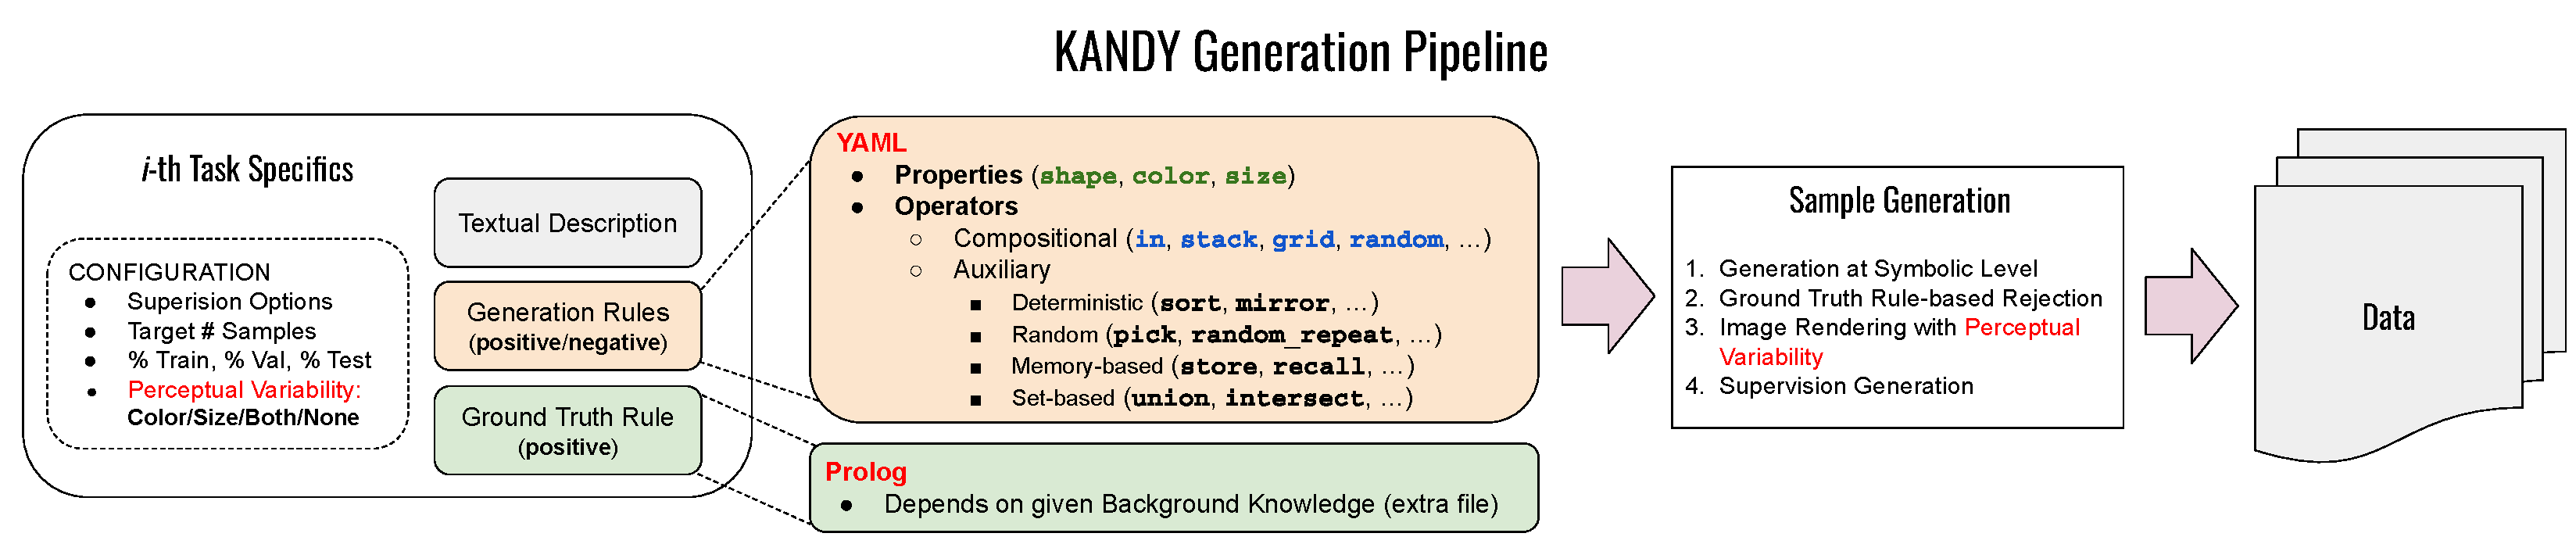
\includegraphics[width=1.0\textwidth]{imgs/kandy/Fig1a.pdf}
\vskip 4mm
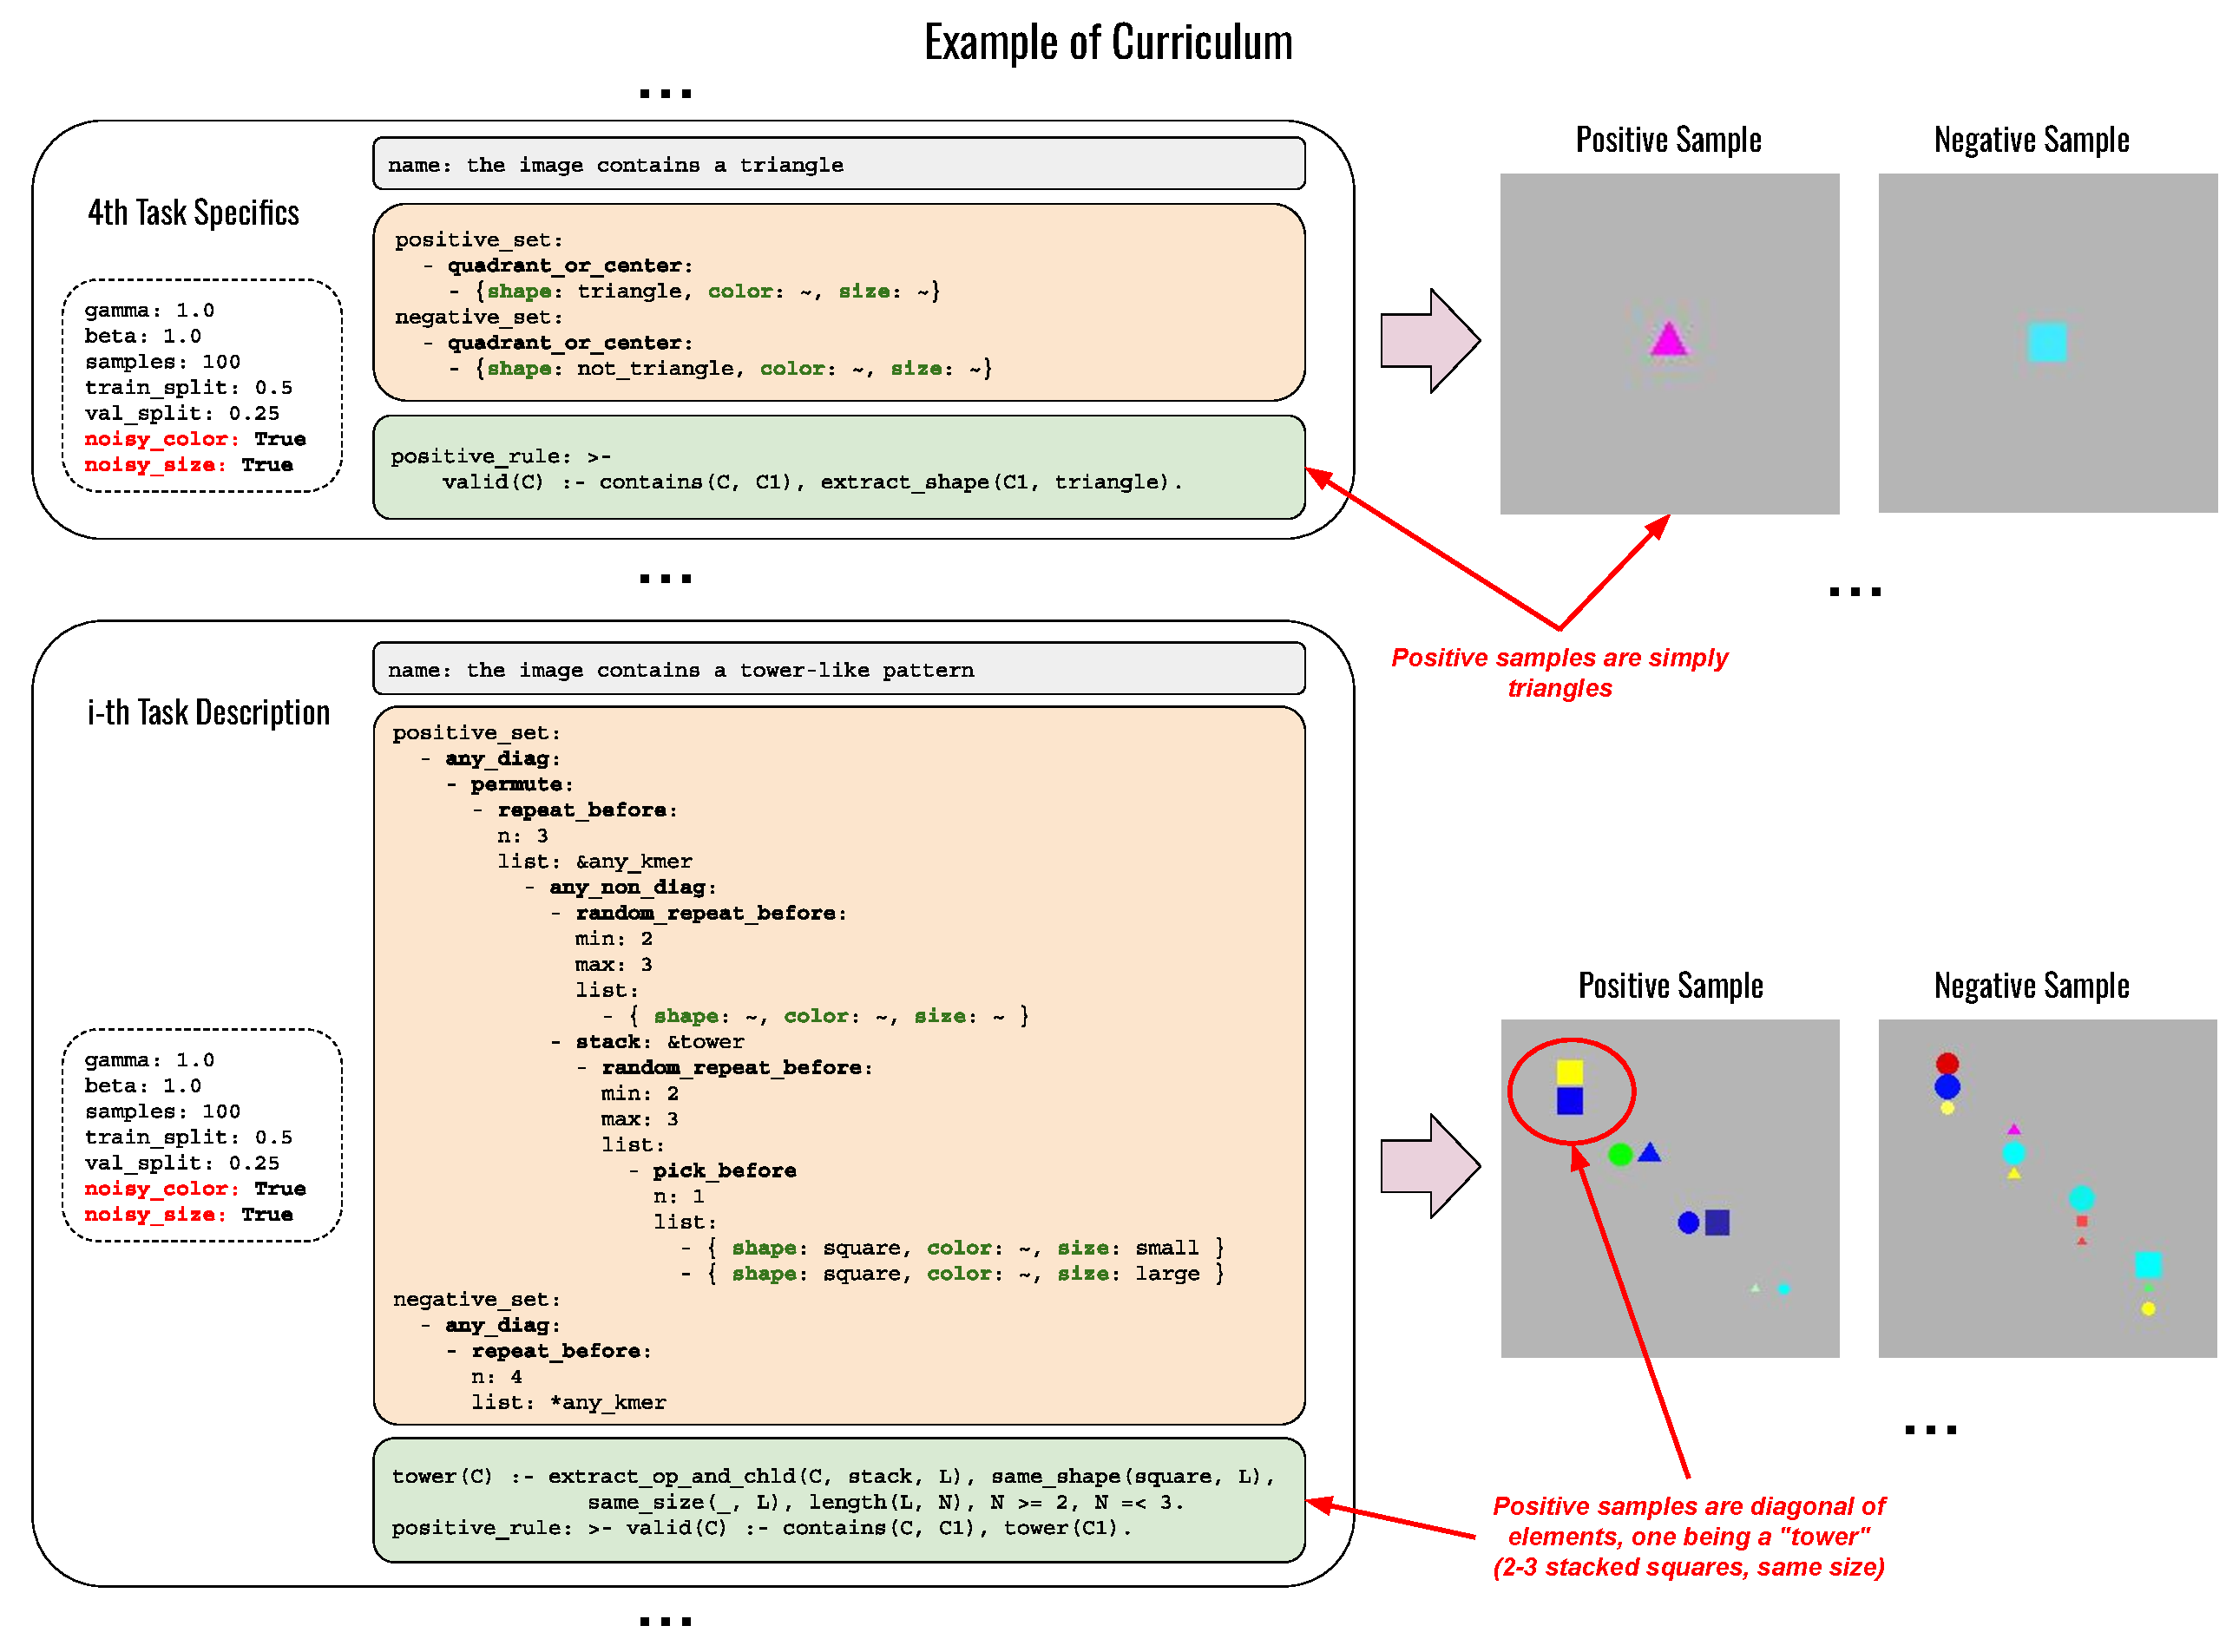
\includegraphics[width=\textwidth]{imgs/kandy/Fig1b.pdf}
\caption[KANDY generation pipeline]{\textit{Top:} Overview of the KANDY generation pipeline: the user provides task specifics and data is generated. Positive and negative sets are defined via symbolic representations and rendered into synthetic images. The ground truth rule is a propositional clause that can be used to reject samples, and thus explains the task. \textit{Bottom:} Example of two tasks from a curriculum generated with KANDY. \label{kandy:fig:example-kandy}}
\end{figure}

\section{Data Generation}\label{kandy:sec:generation}
%\input{src/generator}

Curricula in \textsc{KANDY} are defined in YAML format as lists of tasks. Each task is characterized by two mandatory descriptions of the positive and negative sets as {\it generation rules}, in the form of lists of perceptual trees, where leaves are atomic shapes, and intermediate nodes are annotated with {\it compositional operators}.  In order to avoid the exhaustive enumeration of each image sample, {\it auxiliary operators} (e.g., randomly selecting between multiple options, copying a subtree in a different location, etc.) can be used to expand the list programmatically.
Optionally, each task can also define a {\it ground truth rule}, which is a Prolog-interpretable $\texttt{valid/1}$ predicate (built on some background knowledge). Collectively, generation and ground truth rules describe the task (Figure~\ref{kandy:fig:example-kandy}, top).
KANDY yields synthetic images containing compositions of simple geometric shapes with several configurable properties: \textit{color}, \textit{shape}, and \textit{size}. %, relative position. 
%Tasks consist in binary classification problems defined by positive and negative sets, optionally filtered by a symbolic rule at sampling time. Curricula are defined as sequences of tasks. 
%
Images correspond each to a perceptual tree from the generation rules, and they are iteratively generated by a sampling procedure. If the ground-truth rule is specified, incoherent trees (i.e., samples from the positive set violating the rule and samples from the negative set satisfying it) are discarded.
%Moreover, the generator allows to corrupt task indices, to investigate the effect of task selection errors in multi-task or continual learning settings.



\paragraph{Sample Generation.} 
Task generation rules are symbolic representations that are handled by \textsc{KANDY} in the form of collections of trees (forests). When rules are parsed and a new tree is generated, it is checked against the set of previously generated symbols (to avoid redundancy) and, optionally, against the ground-truth rule, to guarantee consistency between the generation rules and the ground-truth information. 
%
Then, the data generator tries to build samples that are inherently different at the symbolic level. %, thus strongly emphasizing the symbolic nature of the generation process. 
Symbol sets are built by sampling trees from either positive or negative generation rules, and by grounding their leaves.
Since rules might involve non-deterministic attributes,\footnote{Any value (\texttt{\textasciitilde}), negation (\texttt{not\_*}), and disjunction (\texttt{a|b|\dots|k}).} a value is randomly assigned to each of the ungrounded attributes. %selects their values.
Finally, perceptual variability is introduced when the image is generated from its symbolic representation, slightly altering size and color. 
%
%A task is defined by two sets (positive and negative) of symbolic representations, in the form of forests (collections of trees). For each task, when a new tree is generated, it is checked against the set of previously generated symbols (to avoid redundancy) and, optionally, against a user-defined rule (to guarantee consistency). %%Such rule is defined as a Prolog-interpretable $\texttt{valid/1}$ predicate.
%
%A sample is rejected either if it has already been generated (rejection by repetition), or if its sampling set is discordant with the rule (i.e., a sample from the positive set does not satisfy the rule, or a sample from the negative set satisfies it, rejection by rule). The maximum number of rejections is governed by a patience hyper-parameter.
The sampling process is repeated until the target number of examples is produced, unless too many samples are rejected consecutively (controlled via a patience hyper-parameter). In such case, the target size is achieved at rendering time by sampling trees with replacement.
%
%Symbol sets are built by sampling trees from either positive or negative sets, and grounding their leaves.
%Grounding randomly selects values for non-deterministic attributes: any (\texttt{\textasciitilde}), negation (\texttt{not\_*}) , and disjunction (\texttt{a|b|\dots|k}).
%
Symbols are then rendered as images and disjointly split into training, validation and test sets.
%Training, validation and test sets are then built by rendering each symbol into an image, and then disjointly splitting samples according to the target percentages. 
%Examples of generation rules, ground truth, and generated data for two different tasks of a curriculum are given in Figure~\ref{kandy:fig:example-kandy} (bottom).
Figure~\ref{kandy:fig:example-kandy} (bottom) exemplifies generation rules, ground truth, and generated data for two different tasks of a curriculum. In the first task, positive examples are simply images containing triangles of any size and color. In the second task, the property shared by positive examples is more complex, since it consists in a diagonal of objects, one of which must be a tower, i.e., a stack of 2-3 squares of the same size. As negatives also contain diagonals, displacement alone is insufficient to characterize the positive set.


%In the final phase, exactly $\text{target samples} \cdot \text{split percentage}$ are generated: if patience was not exhausted in the first phase, sampling is performed without replacement (and symbols are guaranteed to be unique in every split), otherwise, sampling is performed with replacement.
%In the former case, splits are naturally balanced between positive and negative labels (thanks to the 0.5 probability of choosing between positive and negative sets), while in the latter, label distribution will be unbalanced in favor of the label with the highest symbolic variability: if both distributions are exhausted after reaching the target number of samples, imbalance will reflect the ratio of variability between positive and negative sets, if either is still capable of providing new samples, label distribution will be a poor proxy of symbol distribution.

\paragraph{Image Rendering.}
%
%\textcolor{red}{Questi valori sono quelli di KANDY, ma il generatore può essere configurato con valori arbitrari (inclusi il colore di sfondo e il numero di classi di colore e dimensione)}
%\textcolor{red}{@MARCO: da rivedere.}
%Perceptual details: these considerations apply AFTER symbol generation, thus they do not affect purely symbolic systems, such as the ILP baselines. AAAAAAAAAA
%
Images are drawn at a customizable resolution after symbol generation and sample rejection phases. The background color can be customized as well, and shapes can take any color from a discrete set of configurable values.
%
Similarly, the size of atomic shapes can be controlled by defining a set of sizes of interest, and such a size is not a function of the level of the hierarchy to which atomic shapes belong.\footnote{If the drawing area is too small to draw an atomic shape, overlaps can happen in crowded or highly hierarchical scenes.}
%
Both size and color can be injected with configurable noise, to implement the already mentioned initial perceptual augmentation.

%We deemed alternative approaches not viable, namely, recursively reducing atomic shapes would have caused the risk of unrecognizable shapes with deep hierarchies and the inhability of assigning clear labels to different sizes (as a small triangle on the first level of a hierarchy could be mistaken for a large triangle on the second level, and so on), and cropping would have, likewise, caused unrecognizable shapes (with the degenerate case of bounding boxes smaller than the largest inscribed square in a triangle/circle degenerating to a square).

%\subsection{Task creation: design choices and constraints}
%
%Explain the criteria that drive the process of creating tasks, and especially tasks with incremental complexity. Here explain the constraints and the rationale that we have used to construct the 2/3 data sets that we release.

\paragraph{Supervisions.} \textsc{KANDY} allows to sparsely attach supervisions in the generated curricula of tasks, a process which is modeled by a customizable law $f$. For each task, samples are sorted accordingly to the way the were generated, and the supervision law is function of the sample index $t$, scaled in $[0, 1]$ (i.e, $t=0$ is the first sample of the task and $t=1$ is the last one). %which is instantiated for each (non-rejected) sample in a given task of the curriculum (different tasks have their own private In progression variable). 
\textsc{KANDY} implements an exponential decay law which is evaluated for each sample, $f(t) = \gamma \cdot e^{-\sigma \cdot t}$, where $\sigma = \log(\gamma \cdot \beta^{-1})$ and $\gamma, \beta \in [0, 1]$ are hyper-parameters which can be independently defined for each task in the curriculum.
Function $f(t)$ is monotonically decreasing and has boundary values $f(0) = \gamma$ and $f(1) = \beta$.
Then, a binary random variable is sampled with probability $P_t = f(t)$. \textsc{KANDY} attaches supervised annotations to the image if and only if such binary random variable returns a positive outcome.
%With this strategy, supervisions are more frequent at the beginning of the learning process, while being gradually reduced through time.
This simple strategy effectively schedules sporadic supervisions in a way which is most beneficial for the learning process: supervisions are more abundant at the beginning, when parameters are far from optimal, and are gradually reduced as learning progresses.
We claim that this strategy offers two main advantages: with only two hyper-parameters it allows to govern the exploration-exploitation trade-off (by assigning different importance to the unsupervised and supervised objectives, respectively, at different time steps), and, in learning settings where annotations are not easily available, it allows to allocate limited labels in an effective order.

\paragraph{Compositional Operators.} Compositional primitives are used to model the generation rules (Figure~\ref{kandy:fig:example-kandy}, top) that allow \textsc{KANDY} to recursively place and display children objects (either atomic shapes or other compositional primitives) within the image, as a function of the bounding boxes of such objects. %, by computing bounding boxes of the appropriate dimensions and positions.
%
%receive from their caller (which is either the root sampler or a compositional primitive above) a bounding box, inside which they can draw: it is their responsibility to compute a new, smaller, bounding box for each of their children for the recursive step, and then draw their returned image at the correct location.
%Each compositional primitive reduces bounding boxes in a way linked to its semantics, however, in every case, bounding boxes have a lower bound equal to the space required to draw the largest atomic object, this limit can cause overlaps when composing too many objects, or drawing deep hierarchies.
%
The simplest operator is called \texttt{in} and it draws a child object at the center of the drawing area.
%
Similarly, operators \texttt{quadrant\_ul, quadrant\_ur, quadrant\_ll, quadrant\_lr}
%do not alter the children bounding boxes, but shift their center to one of the four corners of the parent bounding box, resulting in overlapped, but de-centered, objects.
position the bounding box of an object in one of the four quadrants of the drawing area.
%
The \texttt{random} operator draws children objects at random positions, using greedy sample rejection to avoid overlapping with previously drawn shapes.
%exploits a greedy rejection sampling (using the same patience hyperparameter of the general algorithm) to try producing non-overlapping objects. Each child is drawn at a random position, with the whole space available, but if the pixel-wise intersection of the current child and the previously drawn ones is not empty, the current child's position is rejected and resampled. For simplicity there is no backtracking on already drawn children, this implies that the probability of collisions gets increasingly higher as drawing progresses.
%
Operators \texttt{stack} and \texttt{side\_by\_side} equally split the drawing area available for each child along their primary axis (vertical for \texttt{stack} and horizontal for \texttt{side\_by\_side}), while preserving the secondary axis.
%The secondary axis is not split, e.g., a parent bounding box of $384 \times 384$ pixels is split among 10 \texttt{stack}ed children as 10 $384 \times 38$ bounding boxes.
Objects are drawn left-to-right for \texttt{side\_by\_side} and top-to-bottom for \texttt{stack}.
The variants \texttt{stack\_reduce\_bb} and \texttt{side\_by\_side\_reduce\_bb}, instead, also reduce the secondary axis size. %These four operators can be combined to produce perceptually (and possibly semantically) different types of compositions, such as crosses (e.g., \texttt{stack(A, side\_by\_side(B, C, D), E)}), or ``temporal sequences'' (e.g., \texttt{side\_by\_side\_reduce\_bb(stack(A, B, C), stack(B, C, A), stack(C, A, B))}).
%
The \texttt{diag\_ul\_lr} operator positions children objects from the upper-left corner towards the lower-right, while \texttt{diag\_ll\_ur} arranges childred objects from lower-left to upper-right. %Bounding boxes for diagonal operators are computed by dividing both axes by the number of children. %, e.g., a parent bounding box of $256\times 128$ pixels is split among 5 children as $51\times 26$ pixels bounding boxes.
%
The \texttt{grid} operator computes the smallest $n$ such that $n^2 \leq \#\mathrm{children}$ % and divides the bounding box accordingly. 
and children objects are drawn on an $n \times n$ grid from left to right, filling one row at the time, from top to bottom. Grids are incomplete in case the number of children is not a perfect square.

\paragraph{Auxiliary Operators.}
%
%\textcolor{blue}{L. Abbiamo perso la parte importante degli operatori composizionali, questi descritti sono syntactic sugar per semplificare la definizione dei task...}\textcolor{red}{Non ci ero ancora arrivato, ho aggiunto sotto la 3.1.4 come placeholder...}
%
%Besides the set of primitives defined in the previous section, our framework allows to specify, when designing tasks, also additional operators that are easier to use for humans to build symbolic representations.
\textsc{KANDY} also includes additional human-understandable auxiliary operators that simplify the definition of tasks.
%
These operators are list expansion primitives, which allow for compact definitions, mapping lists into other lists containing only atomic shapes and compositional operators.\footnote{For greater flexibility, list expansions are performed twice, operators whose name includes the \texttt{before} suffix are expanded before grounding the sample tree, while every other operator is expanded after grounding.}
%
%We propose two flavors of list expansion operators: one is applied before grounding atomic shapes, the other after grounding. For instance, given the same input list $[\text{any shape}]$ to the repeating operator applied before or after grounding yields different results: $\text{repeat}(2, [\text{any triangle}]) = [\text{small yellow triangle}, \text{small yellow triangle}]$, compared to $\text{repeat\_before}(2, [\text{any triangle}]) = [\text{small yellow triangle}, \text{large blue triangle}]$.
%We provide a complete description of each operator in the code repository. 
In particular, KANDY provides four families of list expansions: (i.) \textit{deterministic}, (ii.) \textit{random}, (iii.) \textit{memory-based}, and (iv.) \textit{set-based}. %, see also Figure~\ref{kandy:fig:example-kandy} (top).
%
\textit{Deterministic} operators (e.g., sorting or mirroring a list) always produce the same output, for a given input. %, note however that as grounding is always a random process, the final outcome will be randomized if deterministic before-grounding operators are used.
%
\textit{Random} operators may produce different results on the same inputs; their behavior can be parameter-free (e.g., random permutation), or controlled by parameters (e.g., random repetition within a range of values).
%
There are three \textit{memory-based} operators: \texttt{store} and \texttt{store\_before} return the input list itself, but they have the side effect of memorizing it and associating it to a text alias; \texttt{recall} (which can only be applied after grounding, unless in combination with set operators) takes an alias and returns the list previously associated to it.
%
\textit{Set-based} operators have special requirements, as they can only take lists of non-grounded atomic shapes or recalled atomic shapes stored before grounding. They produce a single atomic shape output which is the left-associative application of the set operator to the entire list.\footnote{e.g., $\texttt{intersect}([\texttt{any triangle}, \texttt{any non red}, \texttt{any large object}]) \mapsto \texttt{any triangle} \cap \texttt{any non red} \cap \texttt{any large} = \texttt{large non red triangle}$.} We note that proper care should be taken with intersections, as empty output sets are invalid.

\paragraph{Generation Example.} Let us consider the bottom example of Figure~\ref{kandy:fig:example-kandy}.
Both positive and negative sets possess a single element in their list; however, as they contain \textit{auxiliary operators}, these lists will be expanded during sampling.\footnote{Expansion is performed virtually while sampling, to avoid a combinatorial explosion in memory.}
%
First, as the specification is loaded, the YAML engine will process the anchors (\texttt{\&any\_kmer} and  \texttt{\&tower}), associating their labels to a specific subtree, which is copied syntactically every time the corresponding aliases (\texttt{*any\_kmer}, in the negative set, and \texttt{*tower}, in different tasks not shown in the image) are referenced. This step is performed transparently by the YAML engine before \textsc{KANDY} begins parsing the specification.
%
Then, the sampler performs a first bottom-up pass on each tree, and replaces each \texttt{\_before} auxiliary operator (for the positive set these are: \texttt{pick\_before}, \texttt{random\_repeat\_before}, \texttt{random\_repeat\_before}, \texttt{repeat\_before}). For example, the \texttt{pick\_before} subtree is replaced by selecting a single (\texttt{n: 1}) entry from the list of  provided options.
At this point the positive set will have two trees, one where a leaf is replaced by \texttt{\{shape: square, color: \textasciitilde, size: large\}}, and the other with \texttt{\{shape: square, color: \textasciitilde, size: small\}}. Let us  assume the sampler has selected the first one.
%
In the next step, \textit{non-deterministic attributes} are grounded with one of the possible values. For instance, the leaf \texttt{\{shape: square, color: \textasciitilde, size: large\}} can be grounded with any of the six available colors defined in the global configuration section of the YAML file, for  example, \texttt{\{shape: square, color: yellow, size: large\}}.
%
Finally, the sampler performs a second bottom-up pass, resolving each remaining auxiliary operator (for the positive set, \texttt{any\_non\_diag}, \texttt{permute}, \texttt{any\_diag}, in this order). At this point the original sets (containing a single tree each) virtually contain every possible grounding of perceptual trees and the sampler has selected one from either the positive or negative set. Let us assume the following has been sampled from the positive set:
\vskip 2mm
\begin{verbatim}
diag_ul_lr:
  stack:
    - {shape: square, color: yellow, size: large}
    - {shape: square, color: blue, size: large}
  side_by_side:
    - {shape: circle, color: green, size: large}
    - {shape: triangle, color: blue, size: large}
  side_by_side:
    - {shape: circle, color: blue, size: large}
    - {shape: square, color: blue, size: large}
  side_by_side:
    - {shape: triangle, color: green, size: small}
    - {shape: circle, color: cyan, size: small}  
\end{verbatim}
\vskip 2mm
The ground-truth rule (green box Figure \ref{kandy:fig:example-kandy}, bottom) checks whether the sample should be accepted, by looking for a subtree ($\texttt{contains/2}$) satisfying the predicate $\texttt{tower/1}$. As the tree is indeed valid (the first \texttt{stack} contains two squares of the same size), the image can finally be generated, by introducing small perceptual variability in color and size. The result is the  positive image in the bottom part of Figure \ref{kandy:fig:example-kandy}.


%\subsection{Possible usages and modalities}

%Explain the scenarios in which the benchmark can be used: batch vs. continual, single task vs. multi-task, curriculum vs. random. Also mention the interpretability of results (explanations) as an additional task.


\section{Released Datasets}\label{kandy:sec:curricula}
%\subsection{Released curricula}\label{kandy:sec:curricula}
%As illustrated in the previous subsections, KANDY is a benchmarking framework, that can be exploited to generate novel benchmarks with specific characteristics chosen by developers. Nevertheless,
%To show the potential of KANDY and to issue a challenge that could be taken up by several AI communities, % (e.g., NeSy AI and continual learning), 
%we release two benchmarks in the form of curricula of tasks, that showcase the features available to the end-user. We name the two curricula {\it Easy} and {\it Hard}, due to the different complexity of the involved tasks.
In this section we describe the \textsc{KANDY} datasets released publicly. These consist of (i.) two \textit{temporal induction} datasets, (ii.) two collections of \textit{Bongard problems}, and (iii.) two \textit{concept discovery} datasets.
%
Each sample is a $224 \times 224$ RGB image annotated with: task ID, binary label, supervision state (whether the label should be used in training or if the sample should be treated as unsupervised), and symbolic representation. % (whether it should be considered a supervised sample or whether its label should be used only for evaluation) and the symbolic structure used to generate it.
The symbolic representation is a recursive dictionary of lists representing a tree, i.e., the perceptual tree, as created in the sample generation stage. %, where keys are nodes annotated with compositional operators and values are children. Leaves are dictionaries in the form \texttt{\{shape: SH, color: CO, size: SZ\}}, and they represent atomic objects. 
Concept discovery datasets are additionally annotated with ground truth Boolean concepts generated by Prolog rules applied to each sample.
No list expansion operators appear in symbolic annotations.
%
Atomic objects can be {\it small} or {\it large} ($10 \times 10$ and $25 \times 25$ pixels, respectively), and they can take any of six colors ({\it red}, {\it green}, {\it blue}, {\it cyan}, {\it magenta} and {\it yellow}). Object sizes are corrupted by additive uniform noise in the range $\pm[0, 2]$ pixels, and color is corrupted by zero-mean Gaussian noise in HSV coordinates ($\sigma_H = 0.01, \sigma_S = 0.2, \sigma_V = 0.2$). These values were hand-picked to preserve perceptual boundaries (e.g., humans still perceive the maximally corrupted ``red'' as such). Background is set to gray.


\paragraph{\textsc{KANDY-Induction-1}.} This curriculum consists of $20$ elementary tasks with limited annotations ($100$ samples for each task, split into $50$ training, $25$ validation, and $25$ test samples).
Tasks $0$ to $8$ contain a single object and introduce basic (atomic) shapes ($0$-$2$) and color ($3$-$8$). % (circles, triangles and squares) and color (red, green, blue, cyan, magenta, yellow). 
Positive instances contain an object possessing some target attributes, while negative ones contain an arbitrary object.
%
Tasks $9$ to $12$ introduce simple spatial relations between multiple objects. Namely, in such tasks the rightmost object in a positive sample is always a {\it red triangle}, presented in an increasingly complex context: along with an arbitrary object (task $9$), with multiple arbitrary objects ($10$), multiple objects, one of which is a {\it circle} ($11$), and multiple objects, one of which is {\it blue} ($12$). %\textcolor{red}{We expect a neural network to learn the base feature at task 9 and reuse it for subsequent tasks, given the limited amount of training samples? ML: NON FAREI QUI CONSIDERAZIONI SUI MODELLI.}
%
Tasks $13$ and $14$ present complex inter-object relations without confounders: positives in task $13$ consist of a {\it triangle} and a {\it square} of the same color, positives in task $14$ are {\it palindromes of three objects} (i.e., A B A displaced horizontally).
%
Task $15$ to $19$ introduce ``higher order'' objects, which will be reused for the \textsc{KANDY-Induction-2} curriculum. These objects are (extremely abstract) representations of: {\it houses} (a square below a triangle), {\it cars} (two side-by-side circles of the same size), {\it towers} (two or three stacked squares of the same size), {\it wagons} (two or three side-by-side squares of the same size), and {\it traffic lights} (red, yellow and green circles of the same size stacked). Negative samples are perceptually similar to positives, but violate the ground truth rules. %in this last group of tasks are composed of objects with the same structure as the positives, but violating the given rule (e.g., negatives for the towers task are a stack of two or three arbitrary objects, possibly including squares of different sizes).


\paragraph{\textsc{KANDY-Induction-2}.} This curriculum consists of $18$ tasks requiring complex, incremental reasoning capabilities, designed to be challenging for both neural and symbolic methods.
We provide four versions of this curriculum: small fully supervised ($100$ samples per task, $80$ training, $10$ validation, $10$ test samples), large fully supervised ($1000$ total, $800$ train, $100$ validation, $100$ test samples), and two large versions with sparse annotations (both with $1000$ samples, one has fixed $\gamma=\beta=0.5$ probability of supervision, the other has a decay schedule from $\gamma=0.8$ to $\beta=0.2$ probability).
%, while preserving an incremental nature.
%
Tasks $0$ to $3$ introduce uniform k-mers of two and three objects with a common property. % (these tasks are an extension of task 13 from Easy).
%
Positives in tasks $4$ to $8$ contain the objects introduced at the end of the \textsc{KANDY-Induction-1} curriculum, along with confounders (which were not present in \textsc{KANDY-Induction-1}).
%
Tasks $9$ to $11$ introduce hierarchical reasoning, with a universally quantified rule applied to each of the groups within a grid. Positives of task $9$ contain a {\it grid} whose elements are displaced in {\it diagonal}, such that it exists a {\it shared shape} in every group (e.g., each contains a square). Likewise, in task $10$ the rule universally quantifies the existence of a color and, in task $11$, the rule involves the complex objects defined in the Easy curriculum (thus introducing a 3-level perceptual hierarchy).
%
Task $12$ to $14$ extend the {\it palindrome} task of \textsc{KANDY-Induction-1}: in task $12$, positives are a palindrome of arbitrary size between $3$ and $7$ simple objects, displaced along an arbitrary line (horizontal, vertical or diagonal). Task $13$ introduces the concept of ``{\it pseudo-palindrome}'', defined recursively as a sequence $A B A'$ where $B$ is a pseudo-palindrome, and $A$ and $A'$ share either the same shape or the same color. Positives in task $14$ are pseudo-palindromes where couples $A$ and $A'$ can be either simple or complex objects.
%(for which the previous definition applies), or named objects (which must be identical, following the traditional palindrome definition).
%
Positives in task $15$ contain objects of the same color if their number is {\it odd}, or objects of the same shape if their number is {\it even}.
%
Tasks $16$ and $17$ assess logic implication capabilities on top of complex object recognition. %, with positives in the form ``A implies B''. (i.e., both ``A and B'' and ``not A'' are positive samples).
Positives in task $16$ contain {\it four objects} satisfying $(\text{traffic light} \Rightarrow \text{car}) \vee (\text{house} \Rightarrow \text{tower})$. Task $17$ universally quantifies task 16 on a grid. % of 2-to-4 groups.% extends task 16 on a grid of 2 to 4 groups such as positives have each group satisfying the rule.

%\textcolor{red}{Vincoli reasoning hard? es. dimensione background knowledge + numero predicati regola + numero predicati helper}
%
%\textcolor{red}{Vincoli percettivi hard? es. ammettiamo sovrapposizioni ma solo in named objects riconoscibili?}

\paragraph{\textsc{KANDY-Bongard-1/2}.} Both \textsc{KANDY-Induction} curricula are also released in the form of Bongard problems, with a single image divided in twelve panels for each task. Panels are extracted from the small version of either curriculum, by taking, for each task, the first six positive (rendered on the left portion of the image) and six negative (rendered on the right) samples of the test set, in the order they were generated. Panels are left blank (white) if fewer than six samples of the corresponding label were present in the test set.
We release Bongard problems in three flavors. The first one corresponds to a simple $2\times6$ \textsc{grid} of \textsc{KANDY} images at their original size of  $224 \times 224$ pixels (Figure \ref{kandy:fig:bongard}, left). The other two flavors employ a Foundalis-style\footnote{\url{https://www.foundalis.com/res/diss_research.html}} template (Figure \ref{kandy:fig:bongard}, right), to present \textsc{KANDY} in a way which is perceptually similar to original Bongard problems. \textsc{Foundalis-224} upscales the original template to fit unmodified KANDY images, while \textsc{Foundalis-100} images  are built by downscaling KANDY images to $100\times 100$, which is the panel size in standard Bongard problems.

\begin{figure}
    \centering
    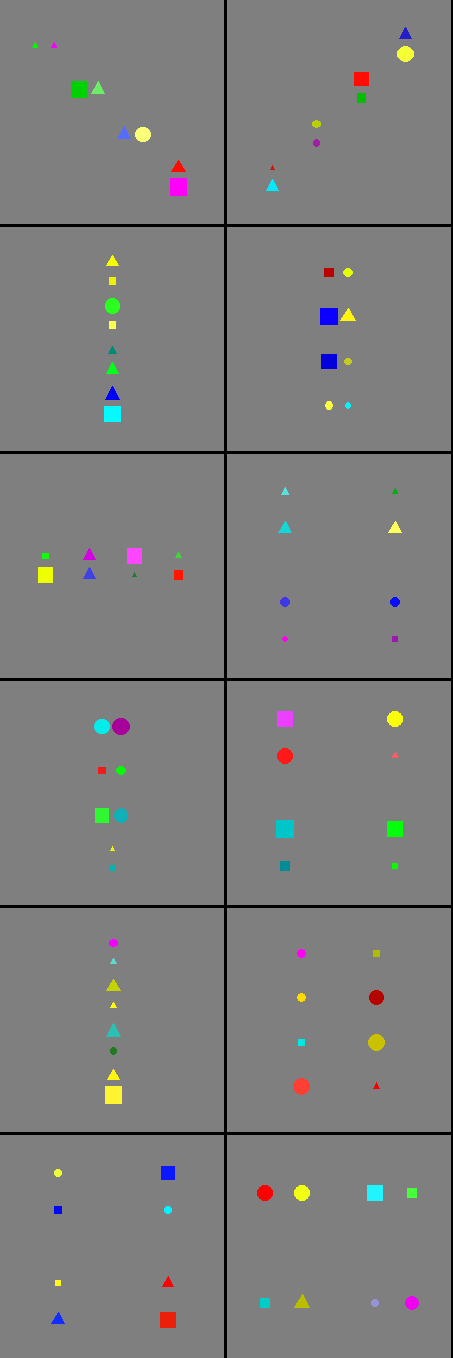
\includegraphics[height=7cm]{imgs/kandy/Fig2a}
    \hfill
    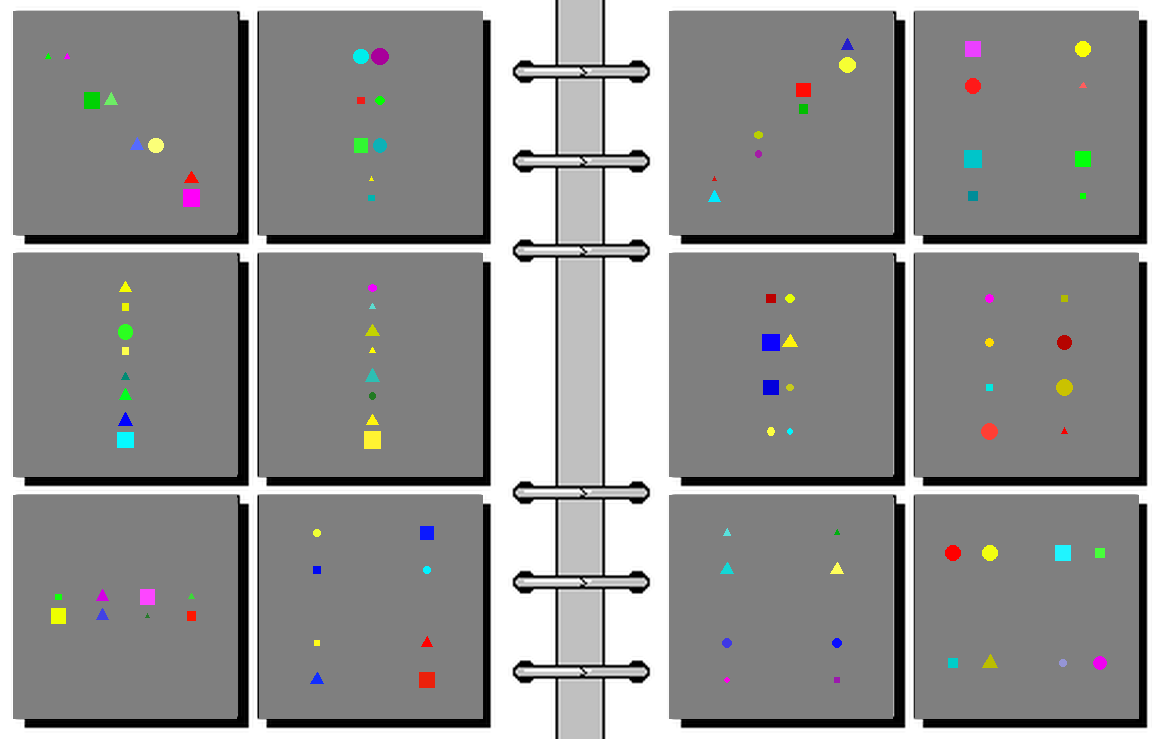
\includegraphics[height=7cm]{imgs/kandy/Fig2b}
    \caption[\textsc{KANDY-Bongard-2} task 4]{\textsc{KANDY-Bongard-2} Task 4, ``There is a house (triangle above a square) somewhere in the image'', in \textsc{grid} (left) and \textsc{Foundalis-224} (right) styles.}
    \label{kandy:fig:bongard}
\end{figure}


\paragraph{\textsc{KANDY-Concepts-1}.}
This curriculum corresponds to \textsc{KANDY-Induction-1}, augmented with concept-level annotations, consisting of elementary attributes (shape, color and size), combined into derived concepts (complex patterns), as highlighted in Table~\ref{cem:tab:kandy_1interactions}. The curriculum is characterized by a warm-up phase (tasks 0 to 8), where only atomic concepts are introduced, followed by a concept-combination phase, in which multiple concepts are combined.

\begin{table}[h]
	\centering
	\resizebox{.7\textwidth}{!}{
		\begin{tabular}{cc|ccc:cccccc:cc}
			\toprule
			\sc Task & \sc Interaction & \multicolumn{3}{c}{\sc Shape} & \multicolumn{6}{c}{\sc Color} & \multicolumn{2}{c}{\sc Size}\\
			&  & \FilledTriangleUp & \FilledSquare & \FilledCircle & \textcolor{red}{\FilledSquare} & \textcolor{green}{\FilledSquare} & \textcolor{blue}{\FilledSquare} & \textcolor{cyan}{\FilledSquare} & \textcolor{magenta}{\FilledSquare} & \textcolor{yellow}{\FilledSquare} & \SmallSquare & \BigSquare \\
			\midrule
			T0   &             & $\exists$    &      &     &      &      &      &      &      &      &     &      \\
			T1   &             &     &  $\exists$    &     &      &      &      &      &      &      &     &      \\
			T2   &             &     &      & $\exists$    &      &      &      &      &      &      &     &      \\
			T3   &             &     &      &     & $\exists$     &      &      &      &      &      &     &      \\
			T4   &             &     &      &     &      & $\exists$     &      &      &      &      &     &      \\
			T5   &             &     &      &     &      &      & $\exists$     &      &      &      &     &      \\
			T6   &             &     &      &     &      &      &      & $\exists$     &      &      &     &      \\
			T7   &             &     &      &     &      &      &      &      & $\exists$     &      &     &      \\
			T8   &             &     &      &     &      &      &      &      &      & $\exists$     &     &      \\
			\hdashline
			T9   &  Binding        & $\exists$    &      &     & $\exists$     &      &      &      &      &      &     &      \\
			T10  &  Binding            & $\exists$    &      &     & $\exists$     &      &      &      &      &      &     &      \\
			T11  &  Binding, AND            & $\exists$    &      & $\exists$    & $\exists$     &      &      &      &      &      &     &      \\
			T12  &  Binding, AND            & $\exists$    &      &     & $\exists$      &           & $\exists$     &      &      &     &    &  \\
			T13  &  Binding           & $\exists$    & $\exists$     &     & \cmark     & \cmark     & \cmark     & \cmark     & \cmark     & \cmark     &     &      \\
			T14  & Complex            & \cmark    & \cmark     & \cmark    & \cmark     & \cmark     & \cmark     & \cmark     & \cmark     & \cmark     & \cmark    & \cmark     \\
			T15  & Pattern & \cmark    & \cmark     &     &      &      &      &      &      &      & \cmark    &  \cmark    \\
			T16  & Pattern &     &      & \cmark    & \cmark     & \cmark     & \cmark     & \cmark     & \cmark     & \cmark     & \cmark    & \cmark     \\
			T17  & Pattern &     & \cmark     &     &      &      &      &      &      &      & \cmark    & \cmark     \\
			T18  & Pattern &     & \cmark     &     &      &      &      &      &      &      & \cmark    & \cmark     \\
			T19  & Pattern &     &      & \cmark    & \cmark     & \cmark     &      &      &      & \cmark     & \cmark    & \cmark     \\
			\bottomrule
	\end{tabular}}
	\caption[\textsc{KANDY-Concepts-1} curriculum]{Concept progression in tasks of \textsc{KANDY-Concepts-1}. When the decision boundary depends on multiple concepts, the type of interaction is summarized by a keyword. Concepts are either existentially quantified ($\exists$) or require task-specific handling (\cmark). The dashed line demarks the point in which we validate our models, as it delimits the boundary between the last task in which elementary concepts are presented and the first complex task.}
	\label{cem:tab:kandy_1interactions}
\end{table}

\paragraph{\textsc{KANDY-Concepts-2}.}
This curriculum, summarized in Table~\ref{cem:tab:kandy_2interactions}, extends \textsc{KANDY-Concepts-1} to a more complex setting. The warm-up phase (tasks 0 to 17) is lengthened to accomodate additional atomic concepts (number of objects and relative alignement of objects within the image), and the concept-combination phase is characterized by concepts which are relations across different objects.
Concepts for task 18 and 19 are simple conjunctions of atomic concepts: a red square, and an blue object combined with another object which is a circle, respectively. Tasks 20 to 24 are characterized by identity relations: every object must have the same shape (20), the same color (21), the same size (22), all the attributes (23), one identical random attribute (24).
The concept associated with task 25 requires every object to have the same color, and at least one of them to be a circle.

\begin{table}[h]
	\centering
	\resizebox{\textwidth}{!}{
		\begin{tabular}{cc|ccc:ccc:ccc:cccccccc}
			\toprule
			\sc Task & \sc Interaction & \multicolumn{3}{c}{\sc Number} & \multicolumn{3}{c}{\sc Alignment} & \multicolumn{3}{c}{\sc Shape} & \multicolumn{6}{c}{\sc Color} & \multicolumn{2}{c}{\sc Size}\\
			&  & \footnotesize one & \footnotesize few & \footnotesize many & \footnotesize diagonal & \footnotesize horizontal & \footnotesize vertical & \FilledTriangleUp & \FilledSquare & \FilledCircle & \textcolor{red}{\FilledSquare} & \textcolor{green}{\FilledSquare} & \textcolor{blue}{\FilledSquare} & \textcolor{cyan}{\FilledSquare} & \textcolor{magenta}{\FilledSquare} & \textcolor{yellow}{\FilledSquare} & \SmallSquare & \BigSquare \\
			\midrule
			T0   &             &  \cmark   &      &     &      &      &      &      &      &      &     &      &      &      &      &      &      &      \\
			T1   &             &     & \cmark     &    &      &      &      &      &      &      &     &      &      &      &      &      &      &      \\
			T2   &             &     & \cmark     &     &      &      &      &      &      &      &     &      &      &      &      &      &      &      \\
			T3   &             &     &      &     & \cmark     &      &      &      &      &      &     &      &      &      &      &      &      &      \\
			T4   &             &     &      &     &      &      & \cmark     &      &      &      &     &      &      &      &      &      &      &      \\
			T5   & OR            &     & \cmark     &      &      &       & \cmark     &      &      &      &     &      &      &      &      &      &      &      \\
			T6   & AND            &     & \cmark     &     & \cmark     &      &      &      &      &      &     &      &      &      &      &      &      &      \\
			T7   &             &     &      &     &      &      &      &  $\exists$    &      &      &     &      &      &      &      &      &      &      \\
			T8   &             &     &      &     &      &      &      &      & $\exists$     &      &     &      &      &      &      &      &      &      \\
			T9   &             &     &      &     &      &      &      &      &      & $\exists$     &     &      &      &      &      &      &      &      \\
			T10  & AND            &     &  \cmark    &     &      &      &      &      & $\forall$     &      &     &      &      &      &      &      &      &      \\
			T11  & OR            &     &      &     &      &      & \cmark     &      &      & $\exists$     &     &      &      &      &      &      &      &      \\
			T12  &             &     &      &     &      &      &      &      &      &      & $\exists$     &      &      &      &      &      &      &      \\
			T13  &             &     &      &     &      &      &      &      &      &      &     & $\exists$     &      &      &      &      &      &      \\
			T14  &             &     &      &     &      &      &      &      &      &      &     &      & $\exists$     &      &      &      &      &      \\
			T15  &             &     &      &     &      &      &      &      &      &      &     &      &      & $\exists$      &      &      &      &      \\
			T16  &             &     &      &     &      &      &      &      &      &      &     &      &      &      & $\exists$     &      &      &      \\
			T17  &             &     &      &     &      &      &      &      &      &      &     &      &      &      &      & $\exists$     &      &      \\
			\hdashline
			T18  & Binding            &     &      &     &      &      &      &      & $\exists$      &      & $\exists$     &      &      &      &      &      &      &      \\
			T19  & AND            &     &      & \cmark     &      &      &      &      &      & $\exists$      &     &      & $\exists$      &      &      &      &      &      \\
			T20  & XOR            &     &      &     &      &      &      & $\forall$     & $\forall$     & $\forall$     &     &      &      &      &      &      &      &      \\
			T21  & XOR            &     &      &     &      &      &      &      &      &      & $\forall$    & $\forall$     & $\forall$     &   $\forall$   & $\forall$     & $\forall$     &      &      \\
			T22  & XOR             &     &      &     &      &      &      &      &      &      &     &      &      &      &      &      & $\forall$     &  $\forall$    \\
			T23  &   Group AND          &     &      &     &      &      &      & $\forall$     & $\forall$     & $\forall$     &  $\forall$   & $\forall$     &  $\forall$    & $\forall$     & $\forall$     & $\forall$     & $\forall$     & $\forall$     \\
			T24  &   Group OR          &     &      &     &      &      &      & $\forall$     & $\forall$     & $\forall$     &  $\forall$   & $\forall$     &  $\forall$    & $\forall$     & $\forall$     & $\forall$     & $\forall$     & $\forall$     \\
			T25  & AND + XOR            &     &      &     &      &      &      &      &      &  $\exists$    & $\forall$    & $\forall$     & $\forall$     & $\forall$     & $\forall$     & $\forall$     &      &      \\
			\bottomrule
		\end{tabular}
	}
	\caption[\textsc{KANDY-Concepts-2} curriculum]{Concept progression in tasks of \textsc{KANDY-Concepts-1}. When the decision boundary depends on multiple concepts, the type of interaction is summarized by a keyword. Concepts are existentially quantified ($\exists$), universally quantified ($\forall$), or require task-specific handling (\cmark). The dashed line demarks the point in which we validate our models, as it delimits the boundary between the last task in which elementary concepts are presented and the first complex task.}
	\label{cem:tab:kandy_2interactions}
\end{table}

\chapter{The LTLZinc Benchmark}
\label{chap:ltlzincbench}

In this chapter we introduce \textsc{LTLZinc}, a benchmarking framework covering a variety of different problems, against which Neuro-symbolic and Continual Learning methods can be evaluated along the temporal and constraint-driven dimensions. Our framework generates expressive Temporal Reasoning and Continual Learning tasks from a Linear Temporal Logic over Finite Traces specification over MiniZinc~\cite{nethercote2007minizinc} constraints, and arbitrary image classification datasets. Fine-grained annotations allow multiple Neural and Neuro-symbolic training regimes on the same generated datasets. \textsc{LTLZinc} is released publicly\footnote{\url{https://github.com/continual-nesy/LTLZinc}} as a generator and as multiple collections of ready-to-use datasets. Experiments of Chapter~\ref{chap:ltlzincseq} and Chapter~\ref{chap:ansya} will rely on such datasets. The content of this chapter is adapted from our IJCAI2025 conference paper~\cite{lorello2025neuro} and our journal paper currently under review at JAIR~\cite{lorello2025ltlzinc}.

\section{\textsc{LTLZinc} at a glance}
\textsc{LTLZinc} positions itself in our taxonomy as a benchmark dealing with \textbf{time-series of images}, covering \textbf{multiple families of tasks} with \textbf{modal} expressivity (relational and temporal logic). Annotations in \textsc{LTLZinc} allow multiple \textbf{reasoning directions}. Data can be observed either in a \textbf{static} or \textbf{continual} fashion, with ground truth which can be either \textbf{given} or \textbf{learned from observations}. Background knowledge remains \textbf{static over time}.
%
The following are the main use cases of \textsc{LTLZinc}:
\begin{enumerate}
	\item \textbf{Learning and Reasoning over Sequences.} \textsc{LTLZinc} can generate datasets of sequences conforming to arbitrary relational-temporal specifications. These can be used as the base for multiple temporal Neuro-symbolic tasks:
	\begin{itemize}
		\item \textbf{Knowledge-driven Sequence Classification.} \textsc{LTLZinc} allows to generate binary Sequence Classification tasks according to known symbolic rules, which can be exploited by a learning agent to make decisions.
		\item \textbf{Temporally-distant Supervision.} Neuro-symbolic Distant Supervision can be performed across multiple steps of reasoning unfolding over time.
		\item \textbf{Constraint Induction over Time.} The relational-temporal nature of \textsc{LTLZinc} specifications allows to induce missing relational knowledge from temporal observations.
	\end{itemize}
	\item \textbf{Continual Learning with Background Knowledge.} \textsc{LTLZinc} can generate a sequence of datasets which generalize Incremental Learning to a broader class of problems with complex temporal behavior. \textsc{LTLZinc} specifications can be exploited as background knowledge for a variety of Continual Learning tasks:
	\begin{itemize}
		\item \textbf{Class-continual Learning.} Novel and already observed classes can be encountered according to complex temporal dynamics.
		\item \textbf{Task-continual Learning.} Curricula of tasks can be defined in terms of task invariants and their temporal behavior.
		\item \textbf{Domain-continual Learning.} Temporal specifications can describe complex stimulus-label mappings evolving over time.
	\end{itemize}
\end{enumerate}

\section{The LTLZinc Framework}\label{ltlzinc:sec:ltlzinc}
We hereby introduce our benchmarking framework for relational and temporal learning and reasoning, covering notation, problem definition, the generation algorithm and its limitations in terms of computational complexity.

\paragraph{Notation.} Let $\gX = \{A: \sX_A, \dots, K: \sX_K\}$ be a set of $K$ \textit{perceptual domains}, each associated to a \textit{symbolic domain} $\gY_j$. As an example, $\gX_A$ and $\gX_B$ could be the domains of MNIST Digits and Fashion-MNIST articles~\cite{xiao2017fmnist}, respectively, whereas $\gY_A$ and $\gY_B$ the corresponding sets of (symbolic) classes. We will indicate with $x_j^{(t)} \in \gX_j$ and $y_j^{(t)} \in \gY_j$ a \textit{perceptual stimulus} and its \textit{symbolic label} observed at discrete time $0 \leq t < T$.
Let $\gC$ be a \textit{mapping of relational constraints over finite domains} from a string identifier to a predicate $\texttt{p/k}$\footnote{Throughout this work, we will consider constraints in $\gC$ to have MiniZinc semantics.} of arity $1 \leq k < K$ between symbolic labels; at each time-step $t$, the tuple of labels $\langle y^{(t)}_A, y^{(t)}_B, \dots, y^{(t)}_{K} \rangle$ corresponding to a certain stimulus $\langle x^{(t)}_A, x^{(t)}_B, \dots, x^{(t)}_{K} \rangle$ may or may not satisfy some predicates in $\gC$.
For instance, let us consider the following example:
\begin{align*}
\gX\colon\quad&A, B, C: [\mathimg{mnist0},\mathimg{mnist9}]\\
 \gY\colon\quad&A, B, C: [0,9]\\
 \gC\colon\quad&\texttt{sum}(A, B, C): A+B=C\\
 &\texttt{same}(A, B, C): \texttt{all\_equal}([A, B, C]).
\end{align*}
We may observe the following perceptual stimuli $\gX^{(t)} = \langle img_A, img_B, img_C\rangle$ (mapped to their corresponding symbolic labels $\gY^{(t)} = \langle A, B, C\rangle$) at four different time-steps $\gX^{(0)} = \langle\mathimg{mnist3}, \mathimg{mnist5},\mathimg{mnist8}\rangle, \gX^{(1)} = \langle\mathimg{mnist2}, \mathimg{mnist5},\mathimg{mnist3}\rangle, \gX^{(2)} = \langle\mathimg{mnist4}, \mathimg{mnist4},\mathimg{mnist4}\rangle, \gX^{(3)} = \langle\mathimg{mnist0}, \mathimg{mnist0},\mathimg{mnist0}\rangle$. For each of them, we can check which relations in $\gC$ hold: $[\{\texttt{sum}: \top, \texttt{same}: \bot\}, \{\texttt{sum}: \bot, \texttt{same}: \bot\}, \{\texttt{sum}: \bot, \texttt{same}: \top\}, \{\texttt{sum}: \top, \texttt{same}: \top\}]$. 
%
Let $\gF$ be a \textit{temporal specification}, defined as an \LTLf formula over the set of relations in $\gC$,  grounded with values in $\gY$. For example, $\gF: \ltlglobally(\texttt{sum}(A,B,C) \leftrightarrow \ltlnext \texttt{same}(A,B,C))$.\footnote{We will omit terms from predicates appearing in $\gF$ (e.g., $\ltlglobally(\texttt{sum} \leftrightarrow \ltlnext \texttt{same})$) when the grounded variables are clear from the context.} This formula models the fact that it will always be true that $\texttt{sum/3}$ is satisfied in a given time-step if and only if the next one satisfies $\texttt{same/3}$. 
The tuple $\langle \gX, \gY, \gC, \gF \rangle$ allows the definition of arbitrary finite-length linear-time first-order reasoning settings.

\paragraph{LTLZinc Problems.} An \textsc{LTLZinc} problem is the tuple $\langle \gX, \gY, \gC, \gF\rangle$, instantiated over a finite time horizon $T$ as a collection of observations in either of two modalities.
In \textbf{sequential mode}, \textsc{LTLZinc} produces a \textit{dataset of sequences}, composed of perceptual stimuli $\gS_\gX = [\langle x_A^{(t)}, \dots, x_{K}^{(t)}\rangle]_{t=0}^{T-1}$, and annotations: $\gS_\gY = [\langle y_A^{(t)}, \dots, y_{K}^{(t)}\rangle]_{t=0}^{T-1}$ (symbolic label annotations), $\gS_\gC = [\langle c_0^{(t)}, \dots, c_{|\gC|-1}^{(t)}\rangle]_{t=0}^{T-1}$ (constraint annotations, $c_i^{(t)} \in \sB$), and $\gL \in \sB$ (sequence label annotation, true if and only if the sequence satisfies $\gF$). Note that the first three are sequential annotations, associated with each time-step of the input stimulus, while the last one is a single binary value associated with the entire sequence. 
%
Conversely, in \textbf{continual mode}, an LTLZinc problem is processed into a \textit{sequence of datasets} $\mathcal{D} = [\langle \gX^{(t)}, \gY^{(t)} \rangle s.t. \gY^{(t)} \models \gC^{(t)}]_{t=0}^{T-1}$, given $[\gC^{(t)}]_{t=0}^{T-1} \models \gF$.
In practice, this means that we first generate a sequence of constraint interpretations satisfying the temporal specification, and then, for each time-step, we sample an image classification dataset $\gD^{(t)} = \langle \gX^{(t)}, \gY^{(t)}\rangle$ coherent with the assignment.
%
In both cases, the problem definition $\langle \gX, \gY, \gC, \gF\rangle$ can be exploited as background knowledge.

\paragraph{Data Generation.} \textsc{LTLZinc} specifications augment \textsc{LTLZinc} problems with auxiliary information.
Arbitrary \textit{dataset splits} can be defined with different characteristics (e.g., a test split can present out-of-distribution images, or additional class labels), by means of \textit{domain mappings}, which associate a split with different datasets $\langle \gX_{split}, \gY_{split}\rangle$.
\textit{Streams} are mappings $variable\_name \mapsto \langle \gX, \gY \rangle$, which allow dynamic associations between perceptual inputs $\langle \gX_i, \gY_i \rangle$ and their grounding in the temporal specification $\gF$, allowing one-to-one, one-to-many or many-to-many associations between variables and perceptual stimuli observed by the agent. Streams allow to model \textit{partial observability over time}, which can be beneficial both to describe incomplete knowledge or to model domain drifts. Given a constraint, e.g., $\texttt{p}(A,B): A = B$, and a formula with stream specifications, e.g., $\texttt{p}(A \mapsto \langle\gX_1, \gY_1\rangle, B \mapsto \langle\gX_2, \gY_2\rangle) \wedge \ltlfinally \texttt{p}(A \mapsto \langle\gX_3, \gY_3\rangle, B \mapsto \langle\gX_4, \gY_4\rangle)$,\footnote{For readability purposes, we will omit stream specifications when the mapping is one-to-one, i.e., $\texttt{p}(A)$ implicitly means $\texttt{p}(A\mapsto\langle\gX_A, \gY_A\rangle)$. In our software, streams are decoupled from temporal formulae, for more readable \textsc{LTLZinc} specification files.} the \textsc{LTLZinc} generator will replace the tuple $(A,B)$ with the domains corresponding to each time-step.\footnote{Internally, different streams applied to the same constraint are converted to different constraints by means of syntactic substitution. The example above is equivalent to $\texttt{p}_0(W,X) \wedge \ltlfinally \texttt{p}_1(Y,Z)$, with $W,X,Y,Z$ belonging to different domains.}
Prior to generation, \textsc{LTLZinc} converts the temporal specification $\gF$ into an Symbolic Finite-state Automaton~\cite{veanes2010symbolic}, by means of an off-the-shelf compiler,\footnote{\url{https://github.com/whitemech/flloat}} the generated automaton is included to the \textsc{LTLZinc} specification as an additional form of background knowledge and it is exploited in the following generation phase.

For both sequential and continual modes, a sequence is generated by means of random walks of length $T$ along the automaton, starting from the initial state. The sequence satisfies the temporal specification (i.e., it is associated with a positive label $\gL = \top$) if and only if the the generated trace ends in an accepting state of the automaton.
Such trace is generated by a $T$-limited randomized depth-first search over the automaton, taking into account \textit{biasing options} which can guide the process to avoid, for example, self-loops at the beginning of a sequence, or, avoid starvation for ``orphan'' constraints, appearing in $\gC$, but not in $\gF$ (meaning that they are known predicates which however do not affect temporal behavior, and thus may never be observed if search is not biased).
For instance, let us consider a dataset consisting of animals, plants and inanimate objects, each associated with a constraint, and a temporal specification indicating that plants will be observed at least once along the sequence. The predicates $\texttt{is\_animal}$ and $\texttt{is\_inanimate}$ are orphans which do not affect the temporal behavior, and act as ``don't care'' values during sampling.\footnote{This means that, when the dataset is used for sequence classification, the notions of ``animal'' and ``inanimate object'' can be safely discarded, however, when the same dataset is used for image classification, they correspond to a subset of the learning targets for which no prior hypothesis is available on their temporal distribution.} At the same time, the automaton associated with the temporal specification is characterized by an accepting sink state which is directly connected to the initial state. Such structure can bias sampling towards non-informative sequences: there is a $0.33\%$ probability of sampling at the first time-step the image of a plant, and every subsequent time-step becomes irrelevant for the sequence label, while we have no guarantee that animals or inanimate objects will be observed at least once by the end of the sequence (i.e., we may have generated a sequence consisting of images of plants only). By counter-biasing the search process, however, we can address both problems, for example, by avoiding sink states with a probability decreased exponentially over time, or by guiding the generator to observe positive instances of all the orphan predicates at least once with a best effort strategy (i.e., if it is impossible to observe all of them along the sequence, optimize for the maximum number of observations).\footnote{Additional biasing options are available in our software.}

Each transition encountered during the search procedure corresponds to an assignment of constraint labels. A MiniZinc instance is built by means of reification of labels in $\gC$ into additional variables, which are constrained to assume values coherent with the transition guard, then the constraint satisfaction problem is solved for the remaining variables (which are assignments for $\gY$ and, possibly, some values of $\gC$ which are irrelevant for the given transition). In order to avoid computing a different solution for every time-step of every sequence, \textsc{LTLZinc} computes all the possible solutions for each transition in the automaton once,\footnote{In order to avoid keeping in memory unnecessary solutions for transitions which are never sampled, \textsc{LTLZinc} performs lazy insertions the first time a new assignment is encountered.} and it stores them in a cache, from which a random solution can be sampled in constant time as often as required.

The main sequence sampling procedure, highlighted so far, is employed differently for sequential and continual generation.
In \textbf{sequential mode}, the generator samples a target number of sequences $N$ for each dataset split. The generated sequences can be either \textit{all positives} (i.e., satisfying the temporal specification), or \textit{balanced positive and negative} sequences.\footnote{Additionally, low level functions in our code can generate a single positive or negative sequence, for experiments on unbalanced datasets.}
A sequential dataset can have sequences of random length within a $\langle min, max\rangle$ (inclusive) range, or fixed length $T$ (corresponding to the range $\langle T, T\rangle$).
The limited depth-first procedure is called $N$ times, each time fixing a random target length $min \leq T' \leq max$ and selecting a target label (positive or negative).
In case the sampled sequence violates the desired target, the procedure backtracks, attempting a different randomized sub-path along the automaton. In case no path of length $T'$ satisfies the target label, successive attempts are made by lowering the sequence length to $T' - 1$, until the minimum value is reached (at which point the task specification cannot be satisfied).
After each sequence in the dataset is generated, a solution for each transition is randomly sampled from the constraint cache, and variables irrelevant for each time-step are assigned arbitrarily. Each sequence in the generated dataset is labeled with: automaton trace (which transitions $s_i\rightarrow s_j$ were sampled), variable assignments (distinguishing irrelevant ones from those required for the transition), constraint values (distinguishing irrelevant and orphan ones from those affecting the transition), and the sequence label.
In \textbf{continual mode}, only a single sequence is sampled. Such sequence is always positive and with a fixed sequence length $T$. Instead of having $N$ different sequences, a continual dataset is characterized by $T$ different episodes, each containing $N$ samples, which are built by extracting $N$ random assignments from the constraint cache. In this case, the sequence of traversed automaton states are a property of the entire dataset, and can be considered a form of background knowledge (i.e., a curriculum of experiences), instead of a sample-level annotation. Seeding the random generator with different values in continual mode will produce different curricula, which however share the property of satisfying the same temporal specification. This can be beneficial when exploring the effect of task ordering in Continual Learning~\cite{mannelli2024tilting}.

\paragraph{Computational Complexity of Generation.}
There are multiple non-polynomial steps involved in the generation of datasets.
As time and space complexities for each stage depend on different quantities, we limit our analysis of the generation procedure to an informal discussion.
%
The conversion between \LTLf and Symbolic Finite-state Automata requires bi-exponential time with respect to the formula length and the output automaton has, in the worst case, a number of states exponential with respect to the number of atomic propositions appearing in the formula, however this step is performed only once during generation and meaningful human-defined formulae tend to be short.
%
The limited depth-first search procedure at the core of sequence sampling has a worst-case running time which is polynomial with respect to the number of potential next states and exponential with respect to the target sequence length, however such case will never be triggered in practice, as it would require an automaton which is fully connected (each state is a successor of every other state) and it is unlikely for an \LTLf formula to be converted to an automaton with such structure. Moreover, the randomized successor sampling step would need to consistently select a next state yielding a failed search every time.
Search is repeated a number of times corresponding to the number of target sequences (i.e., the dataset size for \textbf{sequential mode}, or exactly once for \textbf{incremental mode}).
Each transition of the automaton requires to solve a different Constraint Satisfaction Problem (which is a procedure at least NP-Hard), and, in theory, this process would need to be repeated for each time-step of every sequence.
However, the constraint cache trades-off time for memory requirements. In this way, the number of constraint satisfaction problems to solve, is in the worst case equal to the number of transitions of the automaton (which is in practice much smaller than the theoretical worst case).\footnote{Given the regular structure of transition guards, a straightforward improvement upon the current caching mechanism can be implemented by memorizing partial solutions, and solving smaller Constraint Satisfaction problems as intersections of previously known solutions. We reserve this improvement to future work.}

\section{Sequential Tasks}\label{ltlzinc:sec:seqtasks}
A learning and reasoning agent can exploit a sequential \textsc{LTLZinc} dataset, generated from a specification $\langle \gX, \gY, \gC, \gF \rangle$, in multiple ways. We envision three basic task families, covering a large portion of the temporal and relational reasoning spectrum.
For all three, we will consider the following \textsc{LTLZinc} problem as an example:
\begin{align*}
 \gX\colon\quad&A: \left\{\mathimg{mnist0}, \mathimg{mnist1}, \mathimg{mnist2}, \mathimg{mnist3}, \mathimg{mnist4}, \mathimg{mnist5}, \mathimg{mnist6}, \mathimg{mnist7}, \mathimg{mnist8}, \mathimg{mnist9}\right\};\\
 &B: \left\{\mathimg{svhn0}, \mathimg{svhn1}, \mathimg{svhn2}, \mathimg{svhn3}, \mathimg{svhn4}, \mathimg{svhn5}, \mathimg{svhn6}, \mathimg{svhn7}, \mathimg{svhn8}, \mathimg{svhn9}\right\};\\
 &C: \left\{ \mathimg{cifarair}, \mathimg{cifaraut}, \mathimg{cifarbir}, \mathimg{cifarcat}, \mathimg{cifardee}, \mathimg{cifardog}, \mathimg{cifarfro}, \mathimg{cifarhor}, \mathimg{cifarshi}, \mathimg{cifartru}\right\}\\
 \gY\colon\quad&A, B: [0,9]; \\
 &C: \left\{\text{airplane}, \text{automobile}, \text{bird}, \text{cat}, \text{deer}, \text{dog}, \text{frog}, \text{horse}, \text{ship}, \text{truck}\right\}\\
 \gC\colon\quad&\texttt{p}(A, B, C): A = 2 \cdot B \vee B = 2 \cdot C;\\
 &\texttt{q}(A, B): \texttt{all\_different}([A,B]);\\
 &\texttt{r}(C): C \in \left\{\text{bird}, \text{cat}, \text{deer}, \text{dog}, \text{frog}, \text{horse}\right\}\\
 \gF\colon\quad&\ltlfinally r(C) \wedge ((p(A,B,C) \leftrightarrow \ltlnext q(A,B)) \ltluntil r(C)).
\end{align*}
%
The example above exploits three different datasets (MNIST Digits~\cite{lecun1998mnist}, SVHN~\cite{netzer2011reading}, Cifar-10~\cite{krizhevsky2009learning}, two of which are mapped to the same symbolic labels), and three different kinds of constraints.
Relational constraints $\texttt{p/3}$ and $\texttt{q/2}$ link together different symbolic labels, while $\texttt{r/1}$ is a propositional constraint limiting (for the specific time-steps in which it holds true) the possible values of a single variable.\footnote{A propositional constraint can also describe some semantic feature of single symbolic values (e.g., $\texttt{is\_bird}(X): \texttt{has\_wings}(X) \wedge \texttt{has\_beak}(X)$), enabling concept-based temporal reasoning. Internally \textsc{LTLZinc} collates every non-integer symbolic label to a universe enumeration, allowing lexicographic comparisons also across different datasets.} At the same time, $\texttt{p/3}$ is an arbitrary logic-arithmetic expression,\footnote{In MiniZinc, enumerations are cast to integers in lexicographic order, therefore the implicit equivalences $\left\{airplane = 0, automobile = 1, \ldots, truck = 9\right\}$ hold. Predicate $\texttt{p/3}$ can be true, for example, with $A = \text{don't care}, B = 6, C = \text{cat (3)}$.} while $\texttt{q/2}$ is a \textit{global constraint} from the MiniZinc library, associated with well-known semantics ($A \not = B$).
The automaton corresponding to the temporal specification is shown in Figure~\ref{ltlzinc:fig:example-dfa}. From it we can sample image sequences $\gS_\gX$ associated with their corresponding constraint traces $\gS_\gC$, such as the following positive ($\gS_\gX^+, \gS_\gC^+$) and negative ($\gS_\gX^-, \gS_\gC^-$) examples:\footnote{Underscores correspond to ``don't care'' truth assignments. For readability we use the shorthand notation $\texttt{p} \doteq \{\texttt{p}: \top\}, \neg\texttt{p} \doteq \{\texttt{p}: \bot\}$.}
\begin{align*}
	\gS_\gX^+ &= [\langle \mathimg{mnist3},\mathimg{svhn2}, \mathimg{cifartru}\rangle , \langle \mathimg{mnist8},\mathimg{svhn4}, \mathimg{cifaraut}\rangle , \langle \mathimg{mnist2},\mathimg{svhn1}, \mathimg{cifarair}\rangle , \langle \mathimg{mnist3},\mathimg{svhn2}, \mathimg{cifartru}\rangle , \langle \mathimg{mnist5},\mathimg{svhn5}, \mathimg{cifarcat}\rangle ]\\
	\gS_\gC^+ &= [\langle \neg p, \_, \neg r\rangle , \langle p, \neg q, \neg r\rangle , \langle p, \neg q, \neg r\rangle , \langle \neg p, q, \neg r\rangle , \langle \_, \neg q, r\rangle ]\\\\
	\gS_\gX^- &= [\langle \mathimg{mnist3},\mathimg{svhn2}, \mathimg{cifartru}\rangle , \langle \mathimg{mnist8},\mathimg{svhn4}, \mathimg{cifaraut}\rangle , \langle \mathimg{mnist2},\mathimg{svhn1}, \mathimg{cifarair}\rangle , \langle \mathimg{mnist0},\mathimg{svhn0}, \mathimg{cifarair}\rangle , \langle \mathimg{mnist5},\mathimg{svhn5}, \mathimg{cifarcat}\rangle ]\\
	\gS_\gC^- &= [\langle \neg p, \_, \neg r\rangle , \langle p, \neg q, \neg r\rangle , \langle p, \neg q, \neg r\rangle , \langle \_, \neg q, \_\rangle , \langle \_, \_, \_\rangle ].
\end{align*}

\begin{figure}
    \centering
    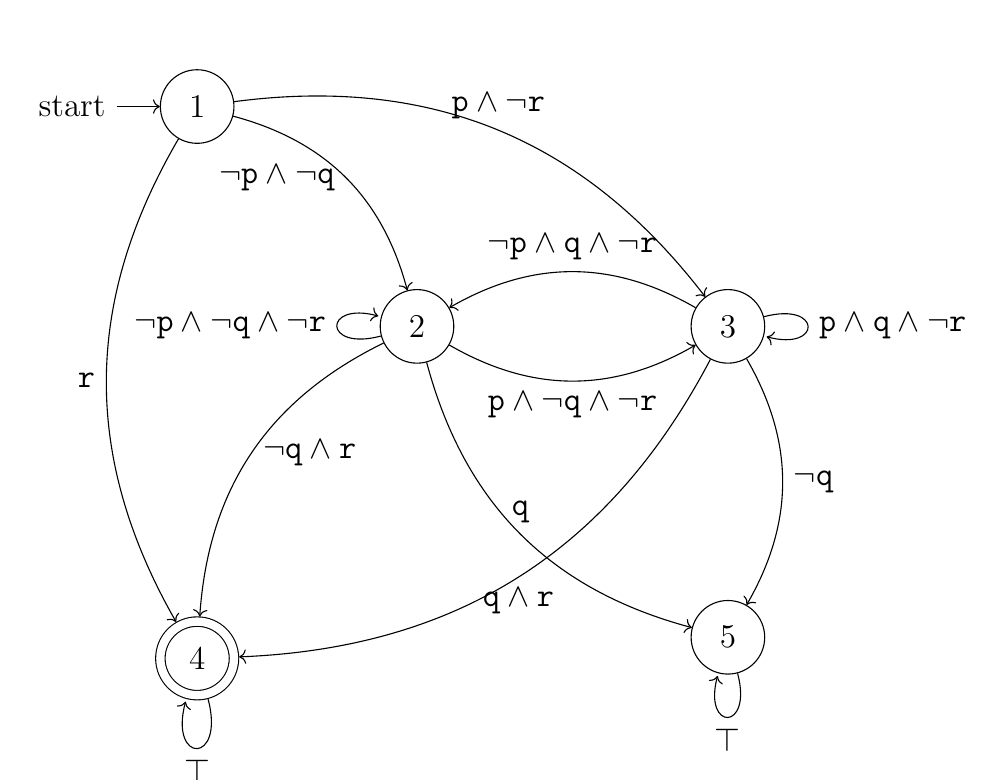
\begin{tikzpicture}[mystate/.style={
          circle, draw, inner sep=6pt 
    },accepting/.style={double distance=3pt, outer sep=1.5pt+\pgflinewidth}]
        \node[mystate, initial] (q1) {$1$};
        \node[mystate, below right=3cm of q1] (q2) {$2$};
        \node[mystate, right=3cm of q2] (q3) {$3$};
        \node[mystate, accepting, below=6cm of q1] (q4) {$4$};
        \node[mystate, below=3cm of q3] (q5) {$5$};

        \path[->]
            (q1) edge[bend left] node[left] {$\neg \texttt{p} \wedge \neg \texttt{q}$} (q2)
            (q1) edge[bend left] node[above] {$\texttt{p} \wedge \neg \texttt{r}$} (q3)
            (q1) edge[bend right] node[left] {$\texttt{r}$} (q4)
            (q2) edge[loop left] node[left] {$\neg \texttt{p} \wedge \neg \texttt{q} \wedge \neg \texttt{r}$} (q2)
            (q2) edge[bend right] node[below] {$\texttt{p} \wedge \neg \texttt{q} \wedge \neg \texttt{r}$} (q3)
            (q2) edge[bend right] node[right] {$\neg \texttt{q} \wedge \texttt{r}$} (q4)
            (q2) edge[bend right] node[above] {$\texttt{q}$} (q5)
            (q3) edge[bend right] node[above] {$\neg \texttt{p} \wedge \texttt{q} \wedge \neg \texttt{r}$} (q2)
            (q3) edge[loop right] node[right] {$\texttt{p} \wedge \texttt{q} \wedge \neg \texttt{r}$} (q3)
            (q3) edge[bend left] node[below] {$\texttt{q} \wedge \texttt{r}$} (q4)
            (q3) edge[bend left] node[right] {$\neg \texttt{q}$} (q5)
            (q4) edge[loop below] node[below] {$\top$} (q4)
            (q5) edge[loop below] node[below] {$\top$} (q5);

    \end{tikzpicture}
    \caption[A Symbolic Finite-state Automaton corresponding to formula $\ltlfinally \texttt{r} \wedge ((\texttt{p} \leftrightarrow \ltlnext \texttt{q}) \ltluntil \texttt{r})$]{A Symbolic Finite-state Automaton for the \LTLf formula $\ltlfinally \texttt{r} \wedge ((\texttt{p} \leftrightarrow \ltlnext \texttt{q}) \ltluntil \texttt{r})$. As $\left\{\texttt{p}, \texttt{q}, \texttt{r}\right\}$ can only assume values in $\sB$, this is in practice a condensed representation of a Deterministic Finite-state Automaton with transitions defined over an alphabet of $2^3$ symbols.}
    \label{ltlzinc:fig:example-dfa}
\end{figure}


\paragraph{Knowledge-driven Sequence Classification.} Given a dataset of positive and negative sequences $\gD \subseteq \gX \times \sB$, sequence classification is the problem of learning a binary classifier $\phi_\vtheta: \gX \mapsto \sB$ from annotated examples, such that the input sequence $\gS_\gX$ is mapped to the positive class if and only if the sequence satisfies $\langle \gX, \gY, \gC, \gF \rangle$. Various degrees of knowledge injection are possible, based on the amount of information from the tuple $\langle \gX, \gY, \gC, \gF \rangle$ and annotations $\langle \gS_\gY, \gS_\gC, \gL\rangle$ available to the learning agent, with end-to-end sequence classification being the weakest (only sequence labels $\gL$ available) and fine-grained supervision at the relational and temporal levels being the strongest (i.e. the entirety of the \textsc{LTLZinc} problem and annotation tuples available). Additionally, the automaton trace annotated at generation time, can be exploited as an oracular source of knowledge, for agents exploiting state-based representations, such as Recurrent Neural Networks, Memory-augmented Neural Networks or Neuro-symbolic Automata~\cite{manginas2024nesya}.
Instantiated in the previous example, a sequence classifier would attempt to learn $\gF$ as ``for a positive sequence, $\texttt{r}$ is guaranteed to be verified eventually, and $\texttt{p}$ and $\texttt{q}$ will alternate in consecutive time-steps, until $\texttt{r}$ is verified''. In order to achieve this objective, knowledge about $\gC$ or $\gY$ might be given, or learned jointly with the sequence label.

\paragraph{Temporally-distant Supervision.}
%The goal of Distant Supervision is to learn a certain number of classifiers $g_i: \gX_i \mapsto \gY_i$, without explicitly providing annotations at the symbolic level $\gY_i$. 
When instantiated over time, Distant Supervision translates into learning all the neural classifiers in a way which satisfies the \textsc{LTLZinc} problem $\langle\gX, \gY, \gC, \gF\rangle$.
Temporally-distant supervision in its ``purest'' form is an extremely weak learning signal, as multiple variable assignments must be learned from sequence-level annotations $\gL$. To overcome this issue, intermediate-level annotations (such as automaton traces, or constraint values) may also be exploited.
In the given example, Temporally-distant Supervision corresponds to learning to classify decimal digits (either with two disjoint mappings for MNIST and SVHN, or employing a joint classifier robust against different perceptual domains) and the ten CIFAR-10 classes, by having access to $\gF$ and $\gC$.
The challenges of Distant Supervision are greatly amplified by the relational and temporal nature of \textsc{LTLZinc}.
Even over finite domains, a single constraint can be satisfied by a number of assignments exponential with the size of domains, and its nature can be more or less subject to the risk of reasoning shortcuts (e.g., \texttt{all\_different} allows any permutation of label mappings, as long as images from the same ground truth label can be mapped to the same shortcut label, while a comparison on the lexicographic ordering of labels has a much smaller, but still non-zero, chance of reasoning shortcuts).
Introducing a temporal component, further increases the size of reasoning shortcuts, as every time-step compounds additional shortcuts (in a multiplicative fashion if constraints holding in consecutive time-steps do not overlap).

\paragraph{Constraint Induction over Time.}
The dictionary of relational constraints $\gC$ can be seen as a collection of inducible predicates in an Inductive Logic Programming setting. However, while in traditional ILP problems predicate semantics is learned directly from observations about their truth values, the goal of constraint induction over time is to learn the semantics of predicates in $\gC^{(t)}$, given indirect observations on sequence labels $\gL$ and image annotations $\gY^{(t)}$. In this setting, traditional ILP examples are provided indirectly by means of temporal knowledge $\gF$: the agent has to perform learning over multiple inducibles at different time-steps, aided by an auxiliary (possibly learned as well) selector function, which dynamically associates each example with the correct target.
Grounding a constraint induction over time task in the provided example, the agent has to learn three different binary functions, one for each of $\{\texttt{p}, \texttt{q}, \texttt{r}\}$. Note that constraints such as $\texttt{p}$ can be significantly harder to learn than $\texttt{q}$ (as it belongs to a library of well-known relations, allowing, for example, brute-force approaches) and $\texttt{r}$ (as it is propositional in nature and the search space is significantly smaller). Difficulty is additionally increased in the case of ambiguities in the temporal behavior (e.g., we are not aware of whether the initial time-step satisfies $r$ or not), as multiple hypotheses need to be considered.
Moreover, as inducible constraints can be observed in a very unbalanced fashion (e.g., because of rare events), the temporal specification can also aid in selecting relevant samples. Observing the automaton corresponding to the provided example (Figure~\ref{ltlzinc:fig:example-dfa}), it is clear that constraint $\texttt{r}$ is heavily unbalanced towards negative observations, as seven transitions require it to be negative, three to be positive, and four do not depend on its truth value, and that positive values are always observed when entering state ``4'' (which is a sink, therefore, after the first observation of a positive $\texttt{r}$, there is no longer any useful temporal information to exploit).

\section{Continual Tasks}\label{ltlzinc:sec:inctasks}
The most popular experimental settings in Continual Learning are \textit{incremental} in nature: agents constantly face new concepts, and are expected to take advantage of the entire learning experience, without being exposed to past experiences a second time. This assumption makes it is possible to benchmark various aspects of an agent learning over time, however it also oversimplifies the temporal behavior a learning agent could be exposed to in the real world.
Assuming we can represent a single learning experience at time-step $t$ as a proposition $\varphi^{(t)} = \text{``the agent is exposed to experience t''}$, \LTLf (or \LTL in infinite-horizon settings, i.e., Lifelong Learning) can model a traditional Incremental Learning setting, solely by exploiting conjunctions and the next operator to define a chain of experiences: %$\gF = \bigwedge\limits_{t = 0}^{T} \ltlnext^{(t)}\varphi^t$, with $\ltlnext^{(t)}$ being the next operator applied $t$ times.
$$\gF = \bigwedge\limits_{t = 0}^{T} \underbracket{\ltlnext \dots \ltlnext}_{t\text{ times}}\varphi^{(t)}.$$
In fact, \LTLf expressivity allows to define behaviors more complex than simple chains of events: experiences can be defined in terms of invariances, eventual guarantees, conditional triggers, and so on. For example, a Continual Learning agent instantiated in an autonomous driving setting, can expect to observe a day-night domain shift, not just once (as popular setups may assume), but repeated periodically, and at the same time, it can assume that certain warning signs correspond to specific dangers in some future time-steps.
\textsc{LTLZinc} allows to define the semantics of each experience $\varphi^{(t)}$ in a way which can be exploited to push Continual Learning research towards a more realistic setting, without sacrificing control over experimental variables.
Moreover, as assumptions, like the ones exemplified above, can be formalized as \textsc{LTLZinc} problems, they can be injected into the learning agent as exploitable knowledge, which can counteract catastrophic forgetting in a targeted fashion.

\paragraph{Class-continual Learning.}
Class-incremental Learning, is an instance of multi-class learning, in which the agent is expected to learn disjoint groups of labels at each episode, being able, by the end of training, to recall all the classes.
\textsc{LTLZinc} can formalize Class-incremental problems by presenting \textbf{disjoint partitions} at each time-step, i.e., by varying the tuple $\langle\gX^{(t)}, \gY^{(t)}\rangle$ dynamically. This can be achieved in two ways, by defining disjoint domains, $\langle\gX^{(0)}, \gY^{(0)}\rangle, \ldots, \langle\gX^{(T-1)}, \gY^{(T-1)}\rangle$, filtered by a single stream over a unary constraint, or by defining a universe domain $\langle\gX, \gY\rangle$, controlled by multiple propositional constraints in the form $\texttt{p}_t = Y \in \gY^{(t)}$, such that $\gY^{(i)} \cap \gY^{(j)} = \varnothing, \forall i \not = j \in \left[0, T\right)$ and $\bigcup\limits_{i = 0}^{T - 1} \gY^{(i)} = \gY$.
For instance, the following is an example of a Class-incremental experience on MNIST Digits, where at each time-step images can belong only to either of two digit labels:
\begin{align*}
 \gX\colon\quad&Y: \left\{\mathimg{mnist0}, \mathimg{mnist1}, \mathimg{mnist2}, \mathimg{mnist3}, \mathimg{mnist4}, \mathimg{mnist5}, \mathimg{mnist6}, \mathimg{mnist7}, \mathimg{mnist8}, \mathimg{mnist9}\right\}\\
 \gY\colon\quad&Y: [0,9]\\
 \gC\colon\quad&\texttt{p}_0(Y): Y \in \left\{0, 1\right\};\\
 &\texttt{p}_1(Y): Y \in \left\{2, 3\right\};\\
 &\texttt{p}_2(Y): Y \in \left\{4, 5\right\};\\
 &\texttt{p}_3(Y): Y \in \left\{6, 7\right\};\\
 &\texttt{p}_4(Y): Y \in \left\{8, 9\right\}\\
 \gF\colon\quad&\texttt{p}_0 \wedge \ltlnext \texttt{p}_1 \wedge \ltlnext\ltlnext \texttt{p}_2 \wedge \ltlnext\ltlnext\ltlnext \texttt{p}_3 \wedge\ltlnext\ltlnext\ltlnext\ltlnext \texttt{p}_4.
\end{align*}
%
Class-incremental learning can be generalized to a setting we call \textbf{Class-continual Learning}, by allowing $\gF$ to be an arbitrary \LTLf formula and by dropping the requirement $\gY^{(i)} \cap \gY^{(j)} = \varnothing, \forall i \not = j \in \left[0, T\right)$.

\paragraph{Domain-continual Learning and Concept Drift.}
In Domain-incremental Learning, the agent learns a single classifier, being presented with perceptual stimuli subject to distribution shift over time. By the end of training, the agent is expected to have good performance regardless of input distribution. \textsc{LTLZinc} can formalize Domain-incremental tasks by means of a single dummy constraint $\texttt{p}(Y) = \top$, with different streams linking it to \textbf{disjoint perceptual domains} $\gX^{(i)} \not = \gX^{(j)} \forall i\not = j$ over time. \textbf{Domain adaptation} experiments can be encoded by allowing perceptual domains to share some images.
The following example models a digit classifier exposed to three different input distributions (MNIST Digits, SVHN and CIFAR-10 interpreted with integer labels).
\begin{align*}
 \gX_{MNIST}\colon\quad&Y: \left\{\mathimg{mnist0}, \mathimg{mnist1}, \mathimg{mnist2}, \mathimg{mnist3}, \mathimg{mnist4}, \mathimg{mnist5}, \mathimg{mnist6}, \mathimg{mnist7}, \mathimg{mnist8}, \mathimg{mnist9}\right\};\\
 \gX_{SVHN}\colon\quad&Y: \left\{\mathimg{svhn0}, \mathimg{svhn1}, \mathimg{svhn2}, \mathimg{svhn3}, \mathimg{svhn4}, \mathimg{svhn5}, \mathimg{svhn6}, \mathimg{svhn7}, \mathimg{svhn8}, \mathimg{svhn9}\right\};\\
 \gX_{CIFAR-10}\colon\quad&Y: \left\{ \mathimg{cifarair}, \mathimg{cifaraut}, \mathimg{cifarbir}, \mathimg{cifarcat}, \mathimg{cifardee}, \mathimg{cifardog}, \mathimg{cifarfro}, \mathimg{cifarhor}, \mathimg{cifarshi}, \mathimg{cifartru}\right\}\\
 \gY\colon\quad&Y: [0, 9]\\
 \gC\colon\quad&\texttt{p}(Y): \top\\
 \gF\colon\quad&\texttt{p}(Y \mapsto \langle\gX_{MNIST}, \gY\rangle) \wedge \ltlnext \texttt{p}(Y\mapsto \langle \gX_{SVHN}, \gY\rangle) \wedge\\ & \ltlnext\ltlnext \texttt{p}(Y \mapsto \langle \gX_{CIFAR-10}, \gY \rangle).
\end{align*}
%
\textbf{Concept drift} is the phenomenon in which the same perceptual stimulus changes semantics over time. It is straightforward to encode concept drift in \textsc{LTLZinc}, by exploiting streams to map the same $\gX$ to different $\gY_i$, for example:
\begin{align*}
 \gX\colon\quad&Y: \left\{ \mathimg{cifarair}, \mathimg{cifaraut}, \mathimg{cifarbir}, \mathimg{cifarcat}, \mathimg{cifardee}, \mathimg{cifardog}, \mathimg{cifarfro}, \mathimg{cifarhor}, \mathimg{cifarshi}, \mathimg{cifartru}\right\}\\
 \gY_0\colon\quad&Y: [0, 9];\\
\gY_1\colon\quad&Y: \left\{airplane, automobile, bird, cat, deer, dog, frog, horse, ship, truck\right\};\\
 \gY_2\colon\quad&Y: \left\{animal, vehicle\right\}\\
 \gC\colon\quad&\texttt{p}(Y): \top\\
 \gF\colon\quad&\texttt{p}(Y \mapsto \langle\gX, \gY_0\rangle) \wedge \ltlnext \texttt{p}(Y\mapsto \langle \gX, \gY_1\rangle) \wedge \ltlnext \ltlnext \texttt{p}(Y\mapsto \langle \gX, \gY_2\rangle).
\end{align*}

\paragraph{Task-continual Learning.}
Task-incremental Learning is an instance of multi-task learning, where the agent is exposed to one task at the time and, by the end of the training experience, it is expected to perform well in all of them. Assuming we can describe a single task by means of an invariance constraint (e.g., a relation linking multiple inputs, which is always true when experiencing the given task), a task-incremental experience can be described by guaranteeing that each constraint is true exactly once. For example, the four modulo-10 arithmetic operations on MNIST Digits can be described as the following \textsc{LTLZinc} problem:\footnote{Formally, for a Task-incremental Learning setting we would also need to assume constraints to be disjoint in time, and $\gF$ such that $p_{add}$ is also false in each time-step except the first one, $p_{sub}$ is false everywhere except the second time-step, and so on.}
\begin{align*}
 \gX\colon\quad&A, B, C: \left\{\mathimg{mnist0}, \mathimg{mnist1}, \mathimg{mnist2}, \mathimg{mnist3}, \mathimg{mnist4}, \mathimg{mnist5}, \mathimg{mnist6}, \mathimg{mnist7}, \mathimg{mnist8}, \mathimg{mnist9}\right\}\\
 \gY\colon\quad&A, B, C: [0,9]\\
 \gC\colon\quad&\texttt{add}(A, B, C): A + B \equiv C \mod{10};\\
 &\texttt{sub}(A, B, C): A - B = C \wedge A \geq B;\\
 &\texttt{mul}(A, B, C): A \cdot B \equiv C \mod{10};\\
 &\texttt{div}(A, B, C): A \div B = C \wedge B \not = 0\\
 \gF\colon\quad&\texttt{add} \wedge \ltlnext \texttt{sub} \wedge \ltlnext\ltlnext \texttt{mul} \wedge \ltlnext\ltlnext\ltlnext \texttt{div}.
\end{align*}
%
Like Class-incremental problems, we can generalize Task-incremental Learning to \textbf{Task-continual Learning}, by allowing arbitrary formulae for $\gF$.
It is important to note that, in this setting, constraints in $\gC$ are \textit{invariance relations}, characterizing the expected input-output behavior, therefore, their labels act as a binary encoding\footnote{If the \textsc{LTLZinc} problem corresponds to a traditional Task-incremental setting, like the example above, this encoding will be one-hot, in general multiple tasks may be active at a given time.} of what is known as \textit{task-id} in the Continual Learning literature, i.e., an oracular descriptor of which task the agent is supposed to solve in the current time-step.
%
In the \textsc{LTLZinc} generator, streams can optionally be annotated with a direction (input/output). Directions do not affect the generation procedure, however they can provide the agent information about which variables are dependent from the others. This is especially useful in Task-continual settings like the proposed example, where uncertainty can be significantly reduced by noting that values for $C$ depend on the assignments of $\langle A, B \rangle$.

\section{Released Sequential Datasets}\label{ltlzinc:sec:seqexp}
%This section presents LTLZinc experiments conducted on six tasks for neuro-symbolic sequence classification over simple perceptual domains and complex relational and temporal knowledge.
In this section we describe the sequential \textsc{LTLZinc} datasets released publicly. We release two collections: (i.) abstract temporal reasoning tasks grounded on synthetic perceptual domains, (ii.) tasks for Neuro-symbolic validation of safety-critical tasks. Every task is annotated with image-level labels, constraint annotations, binary sequence labels, and the trace of automaton states traversed during generation. For each task, biasing options are manually tuned according to the generated automaton topology, in order to minimize the presence of irrelevant subsequences.

\subsection{\textsc{LTLZinc-Sequential-Short/Long}} These collections are characterized by six sequence classification tasks, where positive sequences satisfy the temporal specification, while negative sequences violate it. \textsc{LTLZinc-Sequential-Short} contains sequences between 10 and 20 time-steps, while \textsc{LTLZinc-Sequential-Long} contains longer sequences, between 50 and 100 time-steps. The two collections are otherwise generated from identical \textsc{LTLZinc} specifications. A third collection, \textsc{LTLZinc-Sequential-Short-Legacy}, is generated using an older and less efficient procedure based on rejection sampling, instead of limited depth-first search, but it is otherwise equivalent to \textsc{LTLZinc-Sequential-Short}.
For every collection, 400 sequences are sampled and split into train (320), validation (40) and test (40) splits.
Images are sampled from the MNIST Digits and the Fashion MNIST datasets and rescaled to $32 \times 32$ pixels.

\paragraph{Task 1.} ``It will always be the case that $Y$ is lexicographically smaller than $Z$ if and only if two steps later $V$, $W$ and $Z$ belong to the same class''. This task focuses on comparisons and short term memory capabilities of the agent.
\begin{align*}
	\gX\colon\quad&Y, Z: \{\mathimg{fmnist0}, \mathimg{fmnist1}, \mathimg{fmnist2}, \mathimg{fmnist3}, \mathimg{fmnist4}, \mathimg{fmnist5}, \mathimg{fmnist6}, \mathimg{fmnist7}, \mathimg{fmnist8}, \mathimg{fmnist9}\};\\
	&V, W, X: \{\mathimg{fmnist5}, \mathimg{fmnist6}, \mathimg{fmnist7}, \mathimg{fmnist8}, \mathimg{fmnist9}\}\\
	\gY\colon\quad&Y, Z: \left\{bag, boot, coat, dress, pullover, sandal, shirt, sneaker, top, trouser\right\};\\
	&V, W, X: \left\{sandal, shirt, sneaker, top, trouser\right\}\\
	\gC\colon\quad&\texttt{p}(Y, Z): Y < Z;\\
	&\texttt{q}(V, W, X): \texttt{all\_equal}([V,W,X])\\
	\gF\colon\quad&\ltlglobally (\texttt{p}(Y,Z) \leftrightarrow \ltlnext\ltlnext \texttt{q}(V,W,X)).
\end{align*}
%
The corresponding automaton has 8 states. Self-loops are avoided with a linear decay with rate $0.1$.\footnote{This means that the first time depth-first search encounters a loop state as potential successor, it will discard it from the successors list with probability $1-(0\cdot0.1)$, the second time with probability $1-(1\cdot 0.1)$, and so on. After this pruning step, a successor is sampled uniformly from the list.}

\paragraph{Task 2.} ``It will always be true that, if $Y$ is lexicographically smaller than $Z$ for three consecutive time-steps, then $V$, $W$ and $X$ will share the same labels in the successive step''. This task employes the same domains and constraints of Task 1, but applies them to a different temporal specification, requiring a longer memory window.
\begin{align*}
	\gX\colon\quad&Y, Z: \{\mathimg{fmnist0}, \mathimg{fmnist1}, \mathimg{fmnist2}, \mathimg{fmnist3}, \mathimg{fmnist4}, \mathimg{fmnist5}, \mathimg{fmnist6}, \mathimg{fmnist7}, \mathimg{fmnist8}, \mathimg{fmnist9}\};\\
	&V, W, X: \{\mathimg{fmnist5}, \mathimg{fmnist6}, \mathimg{fmnist7}, \mathimg{fmnist8}, \mathimg{fmnist9}\}\\
	\gY\colon\quad&Y, Z: \left\{bag, boot, coat, dress, pullover, sandal, shirt, sneaker, top, trouser\right\};\\
	&V, W, X: \left\{sandal, shirt, sneaker, top, trouser\right\}\\
	\gC\colon\quad&\texttt{p}(Y, Z): Y < Z;\\
	&\texttt{q}(V, W, X): \texttt{all\_equal}([V,W,X])\\
	\gF\colon\quad&\ltlglobally ((\texttt{p}(Y, Z) \wedge \ltlnext \texttt{p}(Y, Z) \wedge \ltlnext \ltlnext \texttt{p}(Y, Z) \rightarrow\ltlnext\ltlnext\ltlnext \texttt{q}(V, W, X)).
\end{align*}
%
The corresponding automaton has 5 states. Self-loops are avoided with a linear decay with rate $0.1$, while accepting and non-accepting sink states are avoided with a linear decay with rate $0.01$.

\paragraph{Task 3.} ``$X$ will be less than the sum $Y + Z$, up to the point in which the next state has $X$, $Y$ and $Z$ belonging to different classes''. This task requires arithmetic comparisons and is characterized by a challenging temporal behavior (there may be positive sequences satisfying trivially the second constraint twice and never the first).
\begin{align*}
	\gX\colon\quad&X, Y, Z: \left\{\mathimg{mnist0}, \mathimg{mnist1}, \mathimg{mnist2}, \mathimg{mnist3}, \mathimg{mnist4}, \mathimg{mnist5}, \mathimg{mnist6}, \mathimg{mnist7}, \mathimg{mnist8}, \mathimg{mnist9}\right\}\\
	\gY\colon\quad&X, Y, Z: [0, 9]\\
	\gC\colon\quad&\texttt{p}(X, Y, Z): \texttt{all\_different}([X,Y,Z]);\\
	&\texttt{q}(X, Y, Z): X < Y + Z\\
	\gF\colon\quad&\ltlfinally \texttt{p}(X, Y, Z) \wedge (\texttt{q}(X, Y, Z) \ltluntil \ltlnext \texttt{p}(X, Y, Z)).
\end{align*}
%
The corresponding automaton has 5 states. Self-loops are avoided with a linear decay with rate $0.1$, while accepting and non-accepting sink states are avoided with a linear decay with rate $0.01$.

\paragraph{Task 4.} ``$X$ will be less than the sum $Y + Z$, up to the point in which the next state has $X$, $Y$ and $Z$ belonging to different classes''. This task is the same as Task 3, with different perceptual domains (MNIST Digits and FMNIST interpreted as integer classes).
\begin{align*}
	\gX\colon\quad&X: \left\{\mathimg{mnist0}, \mathimg{mnist1}, \mathimg{mnist2}, \mathimg{mnist3}, \mathimg{mnist4}, \mathimg{mnist5}, \mathimg{mnist6}, \mathimg{mnist7}, \mathimg{mnist8}, \mathimg{mnist9}\right\};\\
	&Y, Z: \left\{\mathimg{fmnist0}, \mathimg{fmnist1}, \mathimg{fmnist2}, \mathimg{fmnist3}, \mathimg{fmnist4}, \mathimg{fmnist5}, \mathimg{fmnist6}, \mathimg{fmnist7}, \mathimg{fmnist8}, \mathimg{fmnist9}\right\}\\
	\gY\colon\quad&X, Y, Z: [0, 9]\\
	\gC\colon\quad&\texttt{p}(X, Y, Z): \texttt{all\_different}([X,Y,Z]);\\
	&\texttt{q}(X, Y, Z): X < Y + Z\\
	\gF\colon\quad&\ltlfinally \texttt{p}(X, Y, Z) \wedge (\texttt{q}(X, Y, Z) \ltluntil \ltlnext \texttt{p}(X, Y, Z)).
\end{align*}
%
The corresponding automaton has 5 states. Self-loops are avoided with a linear decay with rate $0.1$, while accepting and non-accepting sink states are avoided with a linear decay with rate $0.01$.

\paragraph{Task 5.} ``$W + X = Y + Z$ is satisfied every other time-step''. This task is characterized by arithmetic reasoning over a simple temporal specification.
\begin{align*}
	\gX\colon\quad&W, X, Y, Z: \left\{\mathimg{mnist0}, \mathimg{mnist1}, \mathimg{mnist2}, \mathimg{mnist3}, \mathimg{mnist4}, \mathimg{mnist5}, \mathimg{mnist6}, \mathimg{mnist7}, \mathimg{mnist8}, \mathimg{mnist9}\right\}\\
	\gY\colon\quad&W, X, Y, Z: [0, 9]\\
	\gC\colon\quad&\texttt{p}(W, X, Y, Z): W + X = Y + Z\\
	\gF\colon\quad&\ltlglobally (\texttt{p}(W,X,Y,Z) \leftrightarrow \ltlweaknext \neg \texttt{p}(W,X,Y,Z)).
\end{align*}
%
The corresponding automaton has 4 states. Self-loops are avoided with a linear decay with rate $0.1$, while accepting and non-accepting sink states are avoided with a linear decay with rate $0.01$.

\paragraph{Task 6.} ``$X + Y = Z$ and $X + Y = 2\cdot Z$ alternate each other''. This task is characterized by arithmetic reasoning over a simple temporal specification.
\begin{align*}
	\gX\colon\quad&X,Y, Z: \left\{\mathimg{mnist0}, \mathimg{mnist1}, \mathimg{mnist2}, \mathimg{mnist3}, \mathimg{mnist4}, \mathimg{mnist5}, \mathimg{mnist6}, \mathimg{mnist7}, \mathimg{mnist8}, \mathimg{mnist9}\right\}\\
	\gY\colon\quad&X, Y, Z: [0, 9]\\
	\gC\colon\quad&\texttt{p}(X, Y, Z): X + Y = Z;\\
	&\texttt{q}(X, Y, Z): X + Y = 2 \cdot Z\\
	\gF\colon\quad&\ltlglobally (\texttt{p}(X,Y,Z) \leftrightarrow \ltlweaknext \neg \texttt{q}(X,Y,Z)).
\end{align*}
%
The corresponding automaton has 4 states. Self-loops are avoided with a linear decay with rate $0.1$, while accepting and non-accepting sink states are avoided with a linear decay with rate $0.01$.


\subsection{\textsc{LTLZinc-Sequential-Safety-Prop/FOL}}
These collections model nine \LTLf patterns~\cite{dwyer1998property} encoding common safety-critical properties. Both collections use the UrbanSound-Spectrogram\footnote{\url{https://github.com/mashrin/UrbanSound-Spectrogram}} dataset, rescaled to $224\times224$ RGB images, as perceptual stimuli, associated with integer classes. Sequences range between 10 and 25 time-steps and each task contains 1000 samples, split into train (800), validation (100) and test (100) sets.
The \textsc{LTLZinc-Sequential-Safety-Prop} and \textsc{LTLZinc-Sequential-Safety-FOL} collections differ only in terms of the constraint dictionary $\gC$, while temporal specifications $\gF$ are homologous for the two collections.

\begin{align*}
	\begin{split}
		\mathcal{X}_{Prop}\colon &Y: \left\{\mathimg{urban_0.png}, \mathimg{urban_1.png}, \mathimg{urban_2.png}, \mathimg{urban_3.png}, \mathimg{urban_4.png}, \mathimg{urban_5.png}, \mathimg{urban_6.png}, \mathimg{urban_7.png}, \mathimg{urban_8.png}, \mathimg{urban_9.png}\right\}\\
		\mathcal{X}_{FOL}\colon &X, Y, Z: \left\{\mathimg{urban_0.png}, \mathimg{urban_1.png}, \mathimg{urban_2.png}, \mathimg{urban_3.png}, \mathimg{urban_4.png}, \mathimg{urban_5.png}, \mathimg{urban_6.png}, \mathimg{urban_7.png}, \mathimg{urban_8.png}, \mathimg{urban_9.png}\right\}\\\\
		\mathcal{Y}_{Prop}\colon &Y: [0, 9]\\
		\mathcal{Y}_{FOL}\colon &X, Y, Z: [0, 9]\\\\
		\mathcal{C}_{Prop}\colon &\texttt{p}(Y): Y < 5;\\ &\texttt{q}(Y): Y \in \{0, 2, 4, 6, 8\};\\
		&\texttt{r}(Y): Y > 5;\\
		&\texttt{s}(Y): Y \in \{1, 3, 5, 7, 9\}\\
		\mathcal{C}_{FOL}\colon &\texttt{p}(X,Y,Z): (X + Y) \mod 10 \equiv Z;\\ &\texttt{q}(X,Y,Z): \texttt{all\_different}([X, Y, Z]);\\
		&\texttt{r}(X,Y,Z): (X < Y \wedge Y < Z) \vee (Z < Y \wedge Y < X);\\
		&\texttt{s}(X,Y,Z): (X = Y \vee Y = Z) \wedge X \not = Z
	\end{split}
\end{align*}

\paragraph{Task 1.} ``\texttt{p} is false before \texttt{q}.''
$$\gF\colon\quad\ltlfinally \texttt{q} \rightarrow \ltlglobally \neg \texttt{p}.$$

\paragraph{Task 2.} ``\texttt{p} is false after \texttt{r}.''
$$\gF\colon\quad\ltlglobally (\texttt{r} \rightarrow \ltlglobally \neg \texttt{p}).$$

\paragraph{Task 3.} ``\texttt{p} is false between \texttt{q} and \texttt{r}.''
$$\gF\colon\quad \ltlglobally ((\texttt{q} \wedge \ltlnext \ltlfinally \texttt{r}) \rightarrow (\neg \texttt{p} \wedge \ltlnext(\neg \texttt{p} \ltluntil \texttt{r}))).$$

\paragraph{Task 4.} ``\texttt{p} is false after \texttt{q} until \texttt{r}.''
$$\gF\colon\quad\ltlglobally (\texttt{q} \rightarrow (\neg \texttt{p} \wedge \ltlnext (\neg \texttt{p} \ltluntil (\texttt{r} \vee \ltlglobally \neg \texttt{p})))).$$

\paragraph{Task 5.} ``\texttt{s} always follows \texttt{p}.''
$$\gF\colon\quad\ltlglobally (\texttt{p} \rightarrow \ltlfinally \texttt{s}).$$

\paragraph{Task 6.} ``\texttt{s} responds to \texttt{p} before \texttt{r}.''
$$\gF\colon\quad(\texttt{p} \rightarrow (\neg \texttt{r} \ltluntil (\texttt{s} \wedge \neg \texttt{r}))) \ltluntil (\texttt{r} \vee \ltlglobally \neg \texttt{r}).$$

\paragraph{Task 7.} ``\texttt{s} responds to \texttt{p} after \texttt{q}.''
$$\gF\colon\quad\ltlglobally (\texttt{q} \rightarrow \ltlglobally (\texttt{p} \rightarrow \ltlfinally \texttt{s})).$$

\paragraph{Task 8.} ``\texttt{s} responds to \texttt{p} between \texttt{q} and \texttt{r}.''
$$\gF\colon\quad\ltlglobally ((\texttt{q} \wedge \ltlnext \ltlfinally \texttt{r}) \rightarrow (\texttt{p} \rightarrow (\neg \texttt{r} \ltluntil (\texttt{s} \wedge \neg \texttt{r}))) \ltluntil \texttt{r}).$$

\paragraph{Task 9.} ``\texttt{s} responds to \texttt{p} after \texttt{q} until \texttt{r}.''
$$\gF\colon\quad\ltlglobally (\texttt{q} \rightarrow ((\texttt{p} \rightarrow (\neg \texttt{r} \ltluntil (\texttt{s} \wedge \neg \texttt{r}))) \ltluntil \texttt{r}) \vee \ltlglobally (\texttt{p} \rightarrow (\neg \texttt{r} \ltluntil (\texttt{s} \wedge \neg \texttt{r})))).$$
%\subsection{Discussion}


\section{Released Continual Datasets}\label{ltlzinc:sec:contexp}
In this section we describe the continual \textsc{LTLZinc} datasets released publicly. We release two Class-continual curricula, instantiated in two variants: \textsc{LTLZinc-Continual-MNIST} (employing MNIST Digits images), and \textsc{LTLZinc-Continual-CIFAR} (based on CIFAR-100).
Task 1 is characterized by the presence of \textit{rare classes}, appearing only once along the agent experience, while Task 2 models classes reappearing cyclically over time.
Every task is generated with 3 different seeds, producing different curricula which are equivalent from the perspective of the temporal specification. Either task is associated with the generated trace along the automaton and the constraint validity for each episode. Each image within an episode is annotated with class labels.
For evaluation purposes, a subset of labels of interest is provided as targets for ``focused'' metrics.

\paragraph{Task 1 MNIST.}
\begin{align*}
 \gX\colon\quad&Y: \left\{\mathimg{mnist0}, \mathimg{mnist1}, \mathimg{mnist2}, \mathimg{mnist3}, \mathimg{mnist4}, \mathimg{mnist5}, \mathimg{mnist6}, \mathimg{mnist7}, \mathimg{mnist8}, \mathimg{mnist9}\right\}\\
 \gY\colon\quad&Y: [0,9]\\
 \gC\colon\quad&\texttt{even}: Y \in \left\{2, 4, 6, 8\right\};\\
 &\texttt{odd}: Y \in \left\{1, 3, 5, 7, 9\right\};\\
 &\texttt{zero}: Y = 0\\
 \gF\colon\quad&\neg \texttt{zero} \wedge (\neg \texttt{zero} \ltluntil (\texttt{zero} \wedge \ltlweaknext \ltlglobally \neg \texttt{zero}).
\end{align*}
Predicates $\texttt{odd}, \texttt{even}$ are orphans, guaranteed to be sampled in positive form at least for one episode along the curriculum (for $100\%$ of the samples inside that episode). Curriculum length: 10 episodes, dataset: 1000 images per episode (800 train, 100 val, 100 test). Focused metrics should refer to predicate $\texttt{zero}$.
Note that since predicate $\texttt{zero}$ corresponds to a single class, the episode in which it appears will be characterized by a \textbf{one-class learning} setting.

\paragraph{Task 1 CIFAR-100.}
\begin{align*}
 \gX\colon\quad&Y: \texttt{CIFAR-100 images}\\
 \gY\colon\quad&Y: \texttt{CIFAR-100 classes}\\
 \gC\colon\quad&\texttt{animals}: Y \in acquatic\_mammals \cup fish \cup insects \cup large\_carnivores \cup \\
 &\quad\quad\quad\quad\quad\quad large\_omnivores\_and\_herbivores \cup reptiles \cup \\
 &\quad\quad\quad\quad\quad\quad non\_insect\_invertebrates \cup  medium\_sized\_mammals \cup \\
 & \quad\quad\quad\quad\quad\quad people \cup small\_mammals;\\
 &\texttt{plants}: Y \in flowers \cup fruit\_and\_vegetables \cup trees;\\
 &\texttt{inanimate}: Y \in food\_containers \cup household\_electrical\_devices \cup \\
 &\quad\quad\quad\quad\quad\quad household\_furniture \cup large\_manmade\_outdoors\_things \cup \\
 &\quad\quad\quad\quad\quad\quad large\_natural\_outdoors\_scenes \cup vehicles\_1 \cup vehicles\_2\\
 \gF\colon\quad&\neg \texttt{plants} \wedge (\neg \texttt{plants} \ltluntil (\texttt{plants} \wedge \ltlweaknext \ltlglobally \neg \texttt{plants}).
\end{align*}
Predicates $\texttt{animals}, \texttt{inanimate}$ are orphans, guaranteed to be sampled in positive form at least for one episode along the curriculum (for $100\%$ of the samples inside that episode). Curriculum length: 50 episodes, dataset: 1000 images per episode (800 train, 100 val, 100 test). Focused metrics should refer to predicate $\texttt{plants}$.
Learning is at the class level (100 targets), predicates are defined in terms of CIFAR-100 superclasses (e.g., $acquatic\_mammals = \left\{beaver, dolphin, otter, seal, whale\right\}$).
Unlike the MNIST version of this task, predicate $\texttt{plants}$ corresponds to multiple classes, therefore, even though they are presented only during a single episode, such episode is still a traditional \textbf{multi-class supervised learning} setting.

\paragraph{Task 2 MNIST.}
\begin{align*}
 \gX\colon\quad&Y: \left\{\mathimg{mnist0}, \mathimg{mnist1}, \mathimg{mnist2}, \mathimg{mnist3}, \mathimg{mnist4}, \mathimg{mnist5}, \mathimg{mnist6}, \mathimg{mnist7}, \mathimg{mnist8}, \mathimg{mnist9}\right\}\\
 \gY\colon\quad&Y: [0,9]\\
 \gC\colon\quad&\texttt{p}: Y \in \left\{0, 1, 2\right\};\\
 &\texttt{q}: Y \in \left\{3, 4, 5\right\};\\
 &\texttt{r}: Y \in \left\{6, 7, 8\right\};\\
 &\texttt{s}: Y = 9.\\
 \gF\colon\quad&\ltlglobally(\texttt{p} \leftrightarrow (\ltlnext \neg \texttt{q} \wedge \ltlnext\ltlweaknext \texttt{q})).
\end{align*}
Predicates $\texttt{r}, \texttt{s}$ are orphans, guaranteed to be sampled in positive form at least for one episode along the curriculum (for $50\%$ of the samples inside that episode). Curriculum length: 20 episodes, dataset: 1000 images per episode (800 train, 100 val, 100 test). Focused metrics should refer to predicates $\texttt{p}, \texttt{q}$.

\paragraph{Task 2 CIFAR-100.}
\begin{align*}
 \gX\colon\quad&Y: \left\{\mathimg{mnist0}, \mathimg{mnist1}, \mathimg{mnist2}, \mathimg{mnist3}, \mathimg{mnist4}, \mathimg{mnist5}, \mathimg{mnist6}, \mathimg{mnist7}, \mathimg{mnist8}, \mathimg{mnist9}\right\}\\
 \gY\colon\quad&Y: [0,9]\\
 \gC\colon\quad&\texttt{animals}: Y \in acquatic\_mammals \cup fish \cup insects \cup large\_carnivores \cup \\
 &\quad\quad\quad\quad\quad\quad large\_omnivores\_and\_herbivores \cup reptiles \cup \\
 &\quad\quad\quad\quad\quad\quad non\_insect\_invertebrates \cup  medium\_sized\_mammals \cup \\
 & \quad\quad\quad\quad\quad\quad people \cup small\_mammals;\\
 &\texttt{plants}: Y \in flowers \cup fruit\_and\_vegetables \cup trees;\\
 &\texttt{inside}: Y \in food\_containers \cup household\_electrical\_devices \cup \\
 & \quad\quad\quad\quad\quad\quad household\_furniture;\\
 &\texttt{outside}: Y \in large\_manmade\_outdoors\_things \cup vehicles\_1 \cup \\
 &\quad\quad\quad\quad\quad\quad  large\_natural\_outdoors\_scenes \cup vehicles\_2.\\
 \gF\colon\quad&\ltlglobally(\texttt{inside} \leftrightarrow (\ltlnext \neg \texttt{outside} \wedge \ltlnext\ltlweaknext \texttt{outside})).
\end{align*}
Predicates $\texttt{animals}, \texttt{plants}$ are orphans, guaranteed to be sampled in positive form at least for one episode along the curriculum (for $50\%$ of the samples inside that episode). Curriculum length: 50 episodes, dataset: 1000 images per episode (800 train, 100 val, 100 test). Focused metrics should refer to predicates $\texttt{inside}, \texttt{outside}$.
Learning is at the class level (100 targets), predicates are defined in terms of CIFAR-100 superclasses.


\part{Time-aware Learning and Reasoning}
\chapter{Inductive Reasoning with \textsc{KANDY}}\label{chap:kandyind}
In this chapter we evaluate {\it neural} and {\it symbolic} approaches against the two \textsc{KANDY-Induction} curricula. In these curricula, the binary classification task can only be solved successfully by agents capable of extracting First-order rules from observations.
The content of this chapter is based on our MLJ journal paper~\cite{lorello2025kandy}.

\section{Neural Experiments}\label{sec:kandy:neur-exp}
We evaluate Neural Networks with respect to their ability to solve the binary classification problems of \textsc{KANDY-Induction}, as a proxy for their sub-symbolic inductive capabilities. The architecture for each experiment consists in a neural backbone $\phi_\vtheta: \sX \mapsto \R^d$, mapping the input image to a latent representation, and one or more classification heads $\psi_{\vtheta'}: \R^d \mapsto [0, 1]$.
We consider the following models as a representative sample of the most widely employed architectures for image classification: (i.) \textit{Multi-layer Perceptrons}, (ii.) \textit{Convolutional Neural Networks}, (iii, iv.) \textit{Residual Networks}~\cite{he2016deep}, and (v.) \textit{Vision Transformers}~\cite{dosovitskiy2020image}.
The effect of time on the learning process is addressed by exploring four different learning settings: (i.) \textit{Independent}, (ii.) \textit{Joint}, (iii.) \textit{Task-incremental}, (iv.) \textit{Continual online}.
Training is performed while sampling positive/negative training data in a class-balanced manner (for each task), thus possibly repeating examples of the least represented category. 
Continual Learning settings are tackled using Experience Replay with Class-balanced Reservoir Sampling~\cite{chrysakis2020online}. The main hyper-parameters are cross-validated by exhaustively searching on fixed grids of values (Appendix~\ref{app:kandyhyper}).

\paragraph{Architectures.} The Multi-layer perceptron (\textsc{MLP}) backbone ($\phi$) consists of a hidden layer with 100 neurons followed by hyperbolic tangent activations, while the Convolutional Neural Network (\textsc{CNN}) backbone is the following architecture:
\begin{verbatim}
Conv2D(features=64, kernel=(5,5), stride=1)
MaxPooling2D()
ReLU()
Conv2D(features=128, kernel=(3,3), stride=2)
MaxPooling2D()
ReLU()
Conv2D(features=256, kernel=(3,3), stride=2)
MaxPooling2D()
Flatten()
Linear(in=5*5*256, out=4096)
Dropout(p=0.1)
\end{verbatim}
Backbones \textsc{ResNet-50} and \textsc{ResNet-50 (H)} are residual networks, where the last layer computes a 4096-dimensional embedding. The former is trained from scratch at each layer, while the latter is initialized with pre-trained weights (ImageNet) and every layer, except the last one, is frozen during training.
Similarly, backbone \textsc{ViT-16 (H)} is a Vision Transformer pre-trained on ImageNet and frozen, with the exception of the last layer.
For every architecture, classification heads ($\psi$) are linear layers with one neuron for each task, equipped with sigmoid activations. 

\paragraph{Learning Settings.} In the \textit{Independent} learning setting, each task is observed in isolation, and the architecture is composed of a single classification head $\psi_{\vtheta'}$, which is re-initialized along with the backbone and trained independently, for each task within the curriculum. This setting corresponds to the baseline performance expected when there is no interaction across tasks.
The architecture implementing the other learning settings is composed of a single backbone, equipped with different classification heads $\psi^{(t)}_{\vtheta'}$ (one for each task in the curriculum). For each of the learning settings, both training and inference data points are annotated with a task-id $t$, to select the correct prediction.\footnote{i.e., $\evy[t] = \psi^{(t)}_{\vtheta'}(\phi^{(t)}_{\vtheta}(\vx))$ for the Independent case, $\evy[t] = \psi^{(t)}_{\vtheta'}(\phi_\vtheta(\vx))$ for every other.}
The \textit{Joint} learning setting is a classic instance of Multi-task Learning, where the whole training data is shuffled and used to optimize both $\phi_\vtheta$ and $\psi^{(t)}_{\vtheta'}$ at once. In this setting, internal representations and weights are shared across each task, without any information loss caused by temporal dynamics.
\textit{Task-incremental} and \textit{Continual online} learning are two instances of Continual Learning, where the architecture observes one task at the time (i.e., for task $t$, we train $\phi_{t;\vtheta} \circ \psi^{(t)}_{\vtheta'}$ and freeze every $\psi^{(t')}$ for $t' \not = t$). In these settings temporal dynamics are expected to cause catastrophic forgetting, but also to guide the learning process thanks to the curricular nature of \textsc{KANDY}.
The \textit{Task-incremental} learning setting allows to shuffle data within a single task and to perform multiple epochs of training, while the \textit{Continual online} learning setting is characterized by a single pass, without altering the order of samples within the dataset.
For each experiment we measure \textsc{Average Accuracy}, \textsc{Average Forgetting}, \textsc{Backward Transfer} and \textsc{Forward Transfer}, at the end of each task.


\begin{table}[t]
	\centering
	\resizebox{\textwidth}{!}{
		\begin{tabular}{lllcccc}
			\toprule 
			\multirow{2}{*}{\textsc{Curriculum}} & \multirow{2}{*}{\textsc{Family}} & \multirow{2}{*}{\textsc{Category}} & \multirow{2}{*}{\textsc{Independent}} & \multirow{2}{*}{\textsc{Joint}} & \multirow{2}{*}{\shortstack[c]{\sc Task\\\sc Incremental}} & \multirow{2}{*}{\shortstack[c]{\sc Continual\\\sc Online}} \\
			& & & & & & \\
			\midrule
			\multirow{10}{*}{\shortstack[c]{\textsc{KANDY-Induction-1}}} & \multirow{5}{*}{\shortstack[c]{Neural}} & \footnotesize \textsc{MLP} & $0.61$ {\tiny ($\pm 0.03$)} & $0.60$ {\tiny ($\pm 0.02$)} & $0.61$ {\tiny ($\pm 0.01$)} & $0.60$ {\tiny ($\pm 0.01$)} \\
			& & \footnotesize \textsc{CNN} & $\textbf{0.72}$ {\tiny ($\pm 0.00$)} & $\textbf{0.73}$ {\tiny ($\pm 0.01$)} & $\textbf{0.74}$ {\tiny ($\pm 0.02$)} & $0.62$ {\tiny ($\pm 0.01$)} \\
			& & \footnotesize \textsc{ResNet-50} & $0.66$ {\tiny ($\pm 0.02$)} & $0.67$ {\tiny ($\pm 0.02$)} & $0.61$ {\tiny ($\pm 0.01$)} & $0.53$ {\tiny ($\pm 0.01$)} \\
			& & \footnotesize \textsc{ResNet-50 (H)} & $\textbf{0.72}$ {\tiny ($\pm 0.02$)} & $0.71$ {\tiny ($\pm 0.02$)} & $0.72$ {\tiny ($\pm 0.02$)} & $\textbf{0.66}$ {\tiny ($\pm 0.01$)} \\
			& & \footnotesize \textsc{ViT (H)} & $0.69$ {\tiny ($\pm 0.01$)} & $0.70$ {\tiny ($\pm 0.01$)} & $0.70$ {\tiny ($\pm 0.01$)} & $0.60$ {\tiny ($\pm 0.03$)} \\
			\cdashline{2-7}
			& \multirow{4}{*}{\shortstack[c]{Symbolic}} & \footnotesize \textsc{Aleph (Nat-Min)} \vphantom{$\sqrt{10}^{2^2}$}& $0.91^{\dagger}$ & -- & -- & -- \\
			& & \footnotesize \textsc{Aleph (Nat-Mid)} & $\textbf{0.96}^{\dagger}$ & -- & -- & -- \\
			& & \footnotesize \textsc{Aleph (Ptr-Min)} & $0.88^{\dagger}$ & -- & -- & -- \\
			& & \footnotesize \textsc{Aleph (Ptr-Mid)} & $0.91^{\dagger}$ & -- & -- & -- \\
			\midrule
			\multirow{10}{*}{\shortstack[c]{\textsc{KANDY-Induction-2}}} & \multirow{5}{*}{\shortstack[c]{Neural}} & \footnotesize \textsc{MLP} & $0.56$ {\tiny ($\pm 0.01$)} & $0.53$ {\tiny ($\pm 0.00$)} & $0.51$ {\tiny ($\pm 0.04$)} & $\textbf{0.55}$ {\tiny ($\pm 0.01$)} \\
			& & \footnotesize \textsc{CNN} & $0.53$ {\tiny ($\pm 0.01$)} & $\textbf{0.57}$ {\tiny ($\pm 0.02$)} & $0.53$ {\tiny ($\pm 0.02$)} & $0.54$ {\tiny ($\pm 0.02$)} \\
			& & \footnotesize \textsc{ResNet-50} & $0.52$ {\tiny ($\pm 0.02$)} & $0.51$ {\tiny ($\pm 0.02$)} & $\textbf{0.54}$ {\tiny ($\pm 0.02$)} & $0.52$ {\tiny ($\pm 0.01$)} \\
			& & \footnotesize \textsc{ResNet-50 (H)} & $\textbf{0.59}$ {\tiny ($\pm 0.03$)} & $\textbf{0.57}$ {\tiny ($\pm 0.02$)} & $0.53$ {\tiny ($\pm 0.02$)} & $0.54$ {\tiny ($\pm 0.01$)} \\
			& & \footnotesize \textsc{ViT (H)} & $0.52$ {\tiny ($\pm 0.03$)} & $0.51$ {\tiny ($\pm 0.01$)} & $0.51$ {\tiny ($\pm 0.05$)} & $0.54$ {\tiny ($\pm 0.01$)} \\
			\cdashline{2-7}
			& \multirow{4}{*}{\shortstack[c]{Symbolic}} & \footnotesize \textsc{Aleph (Nat-Min)} \vphantom{$\sqrt{10}^{2^2}$} & $0.65^{\dagger}$ & -- & -- & -- \\
			& & \footnotesize \textsc{Aleph (Nat-Mid)} & $\textbf{0.66}^{\dagger}$ & -- & -- & -- \\
			& & \footnotesize \textsc{Aleph (Ptr-Min)} & $0.64^{\dagger}$ & -- & -- & -- \\
			& & \footnotesize \textsc{Aleph (Ptr-Mid)} & $0.57^{\dagger}$ & -- & -- & -- \\
			\midrule
			\multirow{5}{*}{\shortstack[c]{\textsc{KANDY-Induction-2}\\Large}} & \multirow{5}{*}{\shortstack[c]{Neural}} & \footnotesize \textsc{MLP} & $0.57$ {\tiny ($\pm 0.02$)} & $0.59$ {\tiny ($\pm 0.01$)} & $0.52$ {\tiny ($\pm 0.01$)} & $0.53$ {\tiny ($\pm 0.01$)} \\
			& & \footnotesize \textsc{CNN} & $0.68$ {\tiny ($\pm 0.00$)} & $\textbf{0.70}$ {\tiny ($\pm 0.01$)} & $0.62$ {\tiny ($\pm 0.01$)} & $0.55$ {\tiny ($\pm 0.01$)} \\
			& & \footnotesize \textsc{ResNet-50} & $\textbf{0.69}$ {\tiny ($\pm 0.00$)} & $0.61$ {\tiny ($\pm 0.01$)} & $0.54$ {\tiny ($\pm 0.03$)} & $0.55$ {\tiny ($\pm 0.02$)} \\
			& & \footnotesize \textsc{ResNet-50 (H)} & $0.56$ {\tiny ($\pm 0.01$)} & $0.59$ {\tiny ($\pm 0.00$)} & $0.56$ {\tiny ($\pm 0.01$)} & $0.56$ {\tiny ($\pm 0.01$)} \\
			& & \footnotesize \textsc{ViT (H)} & $0.63$ {\tiny ($\pm 0.00$)} & $0.65$ {\tiny ($\pm 0.00$)} & $\textbf{0.63}$ {\tiny ($\pm 0.01$)} & $\textbf{0.57}$ {\tiny ($\pm 0.02$)} \\
			\bottomrule
		\end{tabular}
	}
	\caption[Experimental results on \textsc{KANDY-Induction}]{\textsc{KANDY-Induction-1} ({\it top}), \textsc{KANDY-Induction-2} ({\it middle}) and \textsc{KANDY-Induction-2-Large} ({\it bottom}), average accuracy on the test data in different learning settings. Results are averaged ($\pm$ standard deviation) over 3 runs (no standard deviation is reported for deterministic models). 
	Results of symbolic methods are marked with $\dagger$ to recall that, for each example, they were given correct perceptual symbolic features.}
	\label{kandy:tab:acc_easy_hard}    
\end{table}


\section{Symbolic Experiments} We evaluate the Inductive Logic Programming (ILP) capabilities of Aleph\footnote{\url{https://www.cs.ox.ac.uk/activities/programinduction/Aleph}} on \textsc{KANDY-Induction}, testing its capability in devising symbolic explanations of the different tasks (in an atemporal manner), comparing with the available ground truth rules (Section~\ref{app:kandyalephgt} of Appendix~\ref{app:kandyaleph}). 
%
Aleph inductively learns clauses in a specific-to-general setting, so as to cover all the positive examples, without covering any (or, in presence of noise, as few as possible) negative cases. A pruning algorithm finally returns a non-redundant set of such clauses.
%
To model our experimental domain, i.e., to describe with logic predicates the objects in the input scene, we tested two different encodings, namely natural ({\sc\small Nat}) and pointer (\textsc{\small Ptr}), providing a knowledge base of two different sizes (\textsc{\small Min}imal and \textsc{\small Mid}-size, respectively), for a total of four combinations. Each combination is fully described in Appendix~\ref{app:kandyaleph}. 
%
In both encodings, atomic shapes are constants.
%
In the \textsc{\small Nat} encoding, compositional operators are unary functors applied to lists. This corresponds to a one-to-one mapping with the symbolic structure used by the \textsc{KANDY} generator, with the advantage of not requiring modifications to the knowledge base.
%
The \textsc{\small Ptr} encoding, instead, represents compound objects with constants: in this way non-atomic objects are always encoded in a flat fashion and associated with a unique identifier (its pointer), while structure is implicitly built while traversing the knowledge base. A hierarchical structure is encoded by a predicate \texttt{defined\_as/3}, e.g., \texttt{defined\_as(obj\_0001, stack, [obj\_0002, triangle\_red\_small, obj\_0003])}, which defines \texttt{obj\_0001} as a pointer to a vertical stacking of three sub-objects (one atomic, and two defined elsewhere by other \texttt{defined\_as/3} predicates). This encoding has the advantage of not requiring functors, but it splits sample information between knowledge base and example files, requiring an additional \texttt{sample\_is/2} predicate to link them. % needs to encode samples in the KB and link them to the top-level compositional object they depict (with an additional predicate \texttt{sample\_is/2}).
%See supplementary material for more examples.
%
As tasks in either curriculum progressively vary in complexity, with later tasks requiring full First-order Logic reasoning, we tested two scenarios for what concerns the available knowledge base. In the first one, we only allow a \textsc{\small Min}imal knowledge base consisting of $17$ predicates, which is a reasonable starting point for an agnostic learner, aware of the compositional domain, but not of the nature of each task (i.e., predicates in the minimal knowledge base only allow to express containment relations and the existential or universal quantification of a property, such as shape or color, inside a collection).
%
Differently, the \textsc{\small Mid}-size knowledge base contains $39$ predicates, extending the minimal one with list manipulation predicates, arithmetic and compositional object comparisons, and additional predicates related to the task domains (such as checking whether a collection contains identical copies of the same object). 
This knowledge base is the same used to produce compact ground-truth/rejection rules (maximum $6$ literals for each clause) used at generation time, but it is still insufficient without predicate invention capabilities.\footnote{We also experimented with a \textsc{\small large} KB, that extends the \textsc{\small mid}-size one with ``cheating'' predicates, encoding exactly the ground-truth/rejection rules used at task generation. These additional predicates encapsulate non-Horn metapredicates (such as the swi-prolog \texttt{forall/2} predicate), recursive definitions (such as \texttt{pseudo\_palindrome/1}) and complex objects definitions (such as \texttt{is\_house/2}), in theory allowing perfect induction of each task without predicate invention. This last knowledge base is deliberately designed as an upper bound for purely symbolic approaches. However, Aleph fails to produce acceptable solutions for either encoding, as the search space is too large to converge before timeout for most tasks.}
%
All predicates have bounded non-determinacy and can appear in the body of a clause.
%For all six combinations of encodings and KBs, we specify only determinations and data types, leaving language biases as unconstrained as possible.
%With the exception of few intermediate predicates, whose only purpose is to define other predicates in a more compact way, language biases for all six combinations of encoding and KB are unconstrained, allowing for any predicate to appear in a rule any number of times and specifying only determinations and data types.
%
%We train Aleph on the Easy curriculum by allowing a runtime of $30$ minutes for each task, and on the small Hard curriculum with an allowed runtime of $1$ hour per task. The \textsc{\small large} KB fails to produce acceptable solutions for either encoding, as the search space is too large to converge before timeout for most tasks.
%For symbolic experiments, we measure the already introduced micro-accuracy $\mathrm{acc_j}$ for each task, $j=0,\ldots,N-1$, along with the \textsc{\small Average Accuracy}, in order to perform a direct comparison with the neural models.
%
We fix a timeout of 30 minutes for each of the \textsc{KANDY-Induction-1} tasks, and up to one hour for tasks in \textsc{KANDY-Induction-2}.

\begin{table}[t]
	\centering
	\resizebox{\textwidth}{!}{
		\begin{tabular}{llccccc}
			\toprule
			\multirow{2}{*}{\textsc{Curriculum}} & \multirow{2}{*}{\textsc{Category}} & \multirow{2}{*}{\sc \textsc{Correct}} & \footnotesize \sc \multirow{2}{*}{\shortstack[c]{Average\\\sc Precision}} & \footnotesize \sc \multirow{2}{*}{\shortstack[c]{Average\\\sc Recall}} & \multirow{2}{*}{\footnotesize $C_{gt} / C_{\ell t}$} & \multirow{2}{*}{\footnotesize $L_{gt} / L_{\ell t}$} \\
			& & & & & & \\
			\midrule
			\multirow{4}{*}{\shortstack[c]{\textsc{KANDY-Induction-1}}} & \footnotesize \textsc{Aleph (Nat-Min)} & 13/20 & 0.90 & 0.92 & 0.71 & 1.77 \\
			& \footnotesize \textsc{Aleph (Nat-Mid)} & 13/20 &  0.94 & 1.0 & 1.0 & 2.39 \\
			& \footnotesize \textsc{Aleph (Ptr-Min)} & 13/20 & 0.87 & 0.88 & 0.71 & 0.73 \\
			& \footnotesize \textsc{Aleph (Ptr-Mid)} & 13/20 & 0.89 & 0.93 & 0.8 & 0.75 \\
			\hdashline
			\multirow{4}{*}{\shortstack[c]{\textsc{KANDY-Induction-2}}} & \footnotesize \textsc{Aleph (Nat-Min)} & 5/18 & 0.66 & 0.47 & 0.19 & 0.49 \\
			& \footnotesize \textsc{Aleph (Nat-Mid)} & 6/18 & 0.66 & 0.58 & 0.37 & 0.61 \\
			& \footnotesize \textsc{Aleph (Ptr-Min)} & 3/18 & 0.67 & 0.40 & 0.15 & 0.35 \\
			& \footnotesize \textsc{Aleph (Ptr-Mid)} & 3/18 & 0.59 & 0.40 & 0.25 & 0.52 \\
			\bottomrule
		\end{tabular}
	}
	\caption[Aleph performance on \textsc{KANDY-Induction}]{Metrics describing the theories learned by Aleph. Compression ratios are computed as the number of clauses in the ground truth $C_{gt}$ (literals $L_{gt}$, respectively) divided by those in the learned theory $C_{\ell t}$ (literals $L_{\ell t}$, respectively). A value $< 1.0$ indicates an induced theory larger than the ground truth. $L_{\ell t}$ is computed as the maximum number of literals in any clause in a theory.}
\label{kandy:tab:symbolic_results}
\end{table}

\begin{figure}[!ht]
	\iffalse
	%\centering
	\small \hskip 0.4cm \textsc{Task Incremental}\hskip 0.3cm \textsc{Continual Online} \hskip 0.4cm \textsc{Task Incremental}\hskip 0.3cm \textsc{Continual Online} \\
	%\rotatebox{90}{\hskip 1.2cm \textbf{Easy}} \hskip 2.5mm
	\hskip -5mm \includegraphics[height=0.205\textwidth, trim=0.0cm 0.0cm 0cm 0.0cm, clip]{fig/easy/continual_task-avg_accuracy-test-time.pdf}
	%\hskip 2.5mm 
	\includegraphics[height=0.205\textwidth, trim=0.8cm 0.0cm 0cm 0.0cm, clip]{fig/easy/continual_online-avg_accuracy-test-time.pdf}
	%\rotatebox{90}{\hskip 1.2cm \textbf{Hard}}     
	\hskip 1.5mm \includegraphics[height=0.205\textwidth, trim=0.8cm 0.0cm 0cm 0.0cm, clip]{fig/hard_smaller/continual_task-avg_accuracy-test-time.pdf}
	% \hskip 1.5mm 
	\includegraphics[height=0.205\textwidth, trim=0.8cm 0.0cm 0cm 0.0cm, clip]{fig/hard_smaller/continual_online-avg_accuracy-test-time.pdf}
	\fi
	\centering
	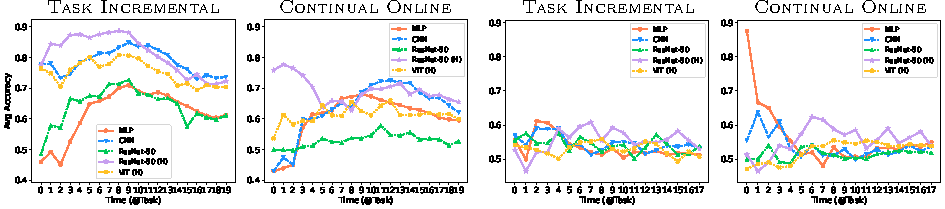
\includegraphics[width=1.0\textwidth]{imgs/kandy/Fig7.pdf}
	%\vskip -1mm
	\caption[Average accuracy over time on \textsc{KANDY-Induction-1}]{\textsc{KANDY-Induction-1} ({\it 1st, 2nd plot}) and \textsc{KANDY-Induction-2} ({\it 3rd, 4th plot}), average accuracy over time (i.e., after having processed data of each of the sequentially streamed tasks). {\it Left}: Task-incremental learning. {\it Right}: Continual online learning.}
	\label{kandy:fig:time_acc_easy_hard}
\end{figure}

\begin{figure}[!ht]
	\iffalse
	\centering  
	\includegraphics[width=0.75\textwidth, trim=0cm 1.1cm 0cm 0.0cm, clip]{fig/easy/independent-acc_matrix-test.pdf}\rotatebox[origin=c]{270}{\hskip -1.6cm \small \textsc{Independent}}\\
	\includegraphics[width=0.75\textwidth, trim=0cm 1.1cm 0cm 0.65cm, clip]{fig/easy/joint-acc_matrix-test.pdf}\rotatebox[origin=c]{270}{\hskip -1.8cm \small \textsc{Joint}}\\    
	\includegraphics[width=0.75\textwidth, trim=0cm 1.1cm 0cm 0.65cm, clip]{fig/easy/continual_task-acc_matrix-test.pdf}\rotatebox[origin=c]{270}{\hskip -1.8cm \small \textsc{Task Incr.}}\\
	\includegraphics[width=0.75\textwidth, trim=0cm 0.2cm 0cm 0.65cm, clip]{fig/easy/continual_online-acc_matrix-test.pdf}\rotatebox[origin=c]{270}{\hskip -2.7cm \small \textsc{Cont. Online}}\\
	\includegraphics[width=0.75\textwidth, trim=0cm 0.2cm 0cm 0.2cm, clip]{fig/sym_easy/independent-Accuracy.pdf}\rotatebox[origin=c]{270}{\hskip -2.7cm \small \textsc{Symbolic}}\\      
	\fi
	\centering
	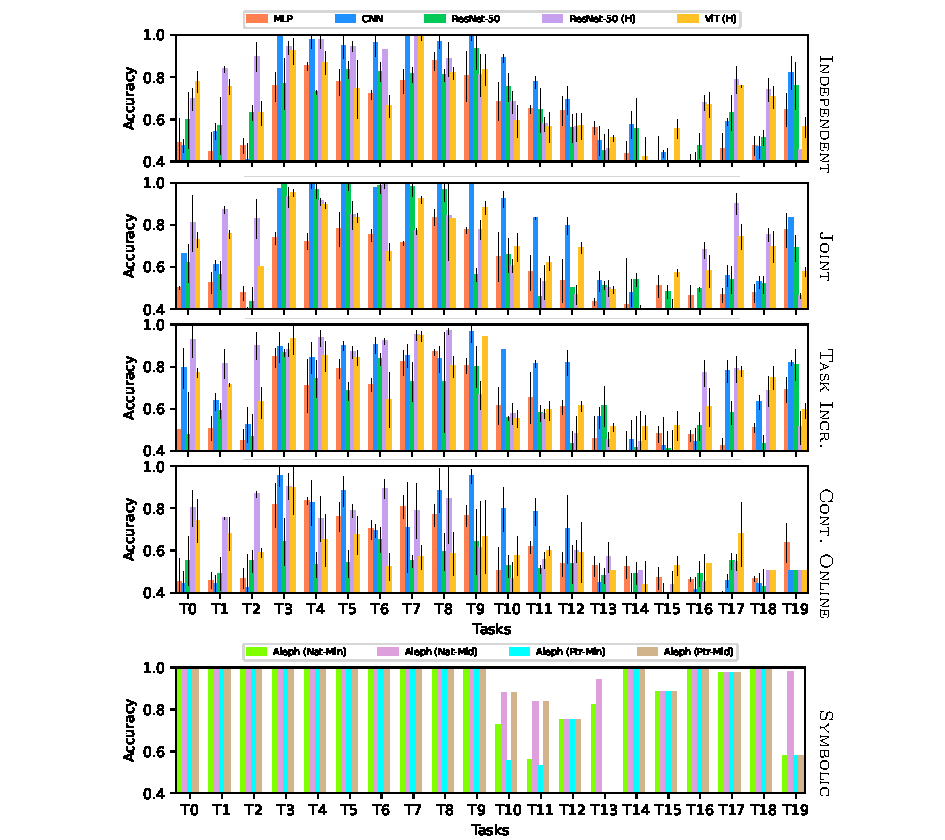
\includegraphics[width=1.0\textwidth]{imgs/kandy/Fig8.pdf}
	%\vskip -1mm
	\caption[Per-task accuracies over time on \textsc{KANDY-Induction-1}]{\textsc{KANDY-Induction-1}, per-task accuracies of the compared models in different learning settings. Neural (first four rows) and symbolic methods (last row) are represented with different colormaps. Models significantly under-performing (below 0.4) are not shown.}
	\label{kandy:fig:acc_per_task_easy}
\end{figure}

\begin{figure}
	\iffalse
	\centering
	\hskip -0.3cm \includegraphics[height=0.205\textwidth]{fig/easy/continual_task-avg_forgetting-test-time.pdf}
	\includegraphics[height=0.205\textwidth]{fig/easy/continual_task-backward_transfer-test-time.pdf}  
	\includegraphics[height=0.205\textwidth]{fig/easy/continual_task-forward_transfer-test-time.pdf}
	\rotatebox{270}{\hskip -2.4cm \small \textsc{Task Incr.}}\\
	\hskip -0.3cm \includegraphics[height=0.205\textwidth]{fig/easy/continual_online-avg_forgetting-test-time.pdf} 
	\includegraphics[height=0.205\textwidth]{fig/easy/continual_online-backward_transfer-test-time.pdf}
	\includegraphics[height=0.205\textwidth]{fig/easy/continual_online-forward_transfer-test-time.pdf}
	\rotatebox{270}{\hskip -2.6cm \small \textsc{Cont. Online}}\\
	\fi
	\centering
	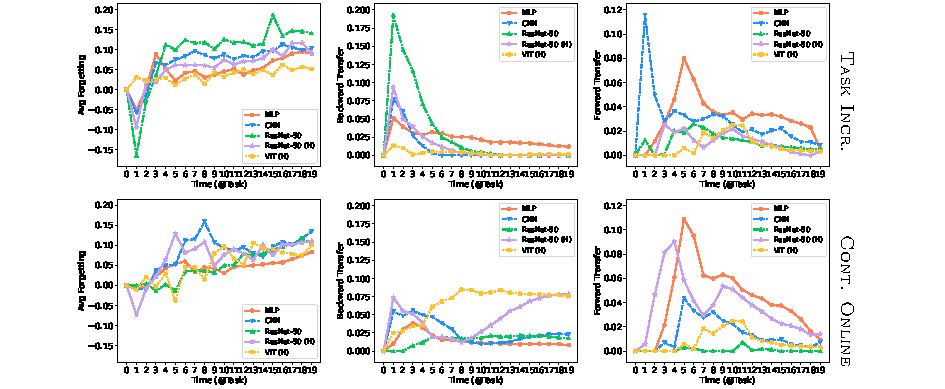
\includegraphics[width=1.0\textwidth]{imgs/kandy/Fig9.pdf}
	%\vskip -1mm
	\caption[Average forgetting over time on \textsc{KANDY-Induction-1}]{\textsc{KANDY-Induction-1}, average forgetting (the lower the better), backward transfer, forward transfer over time (i.e., after having processed data of each of the sequentially streamed tasks). {\it Top}: Task-incremental learning. {\it Bottom}: Continual online learning.}
	\label{kandy:fig:time_easy}
\end{figure}

\begin{figure}[!ht]
	\iffalse
	\centering
	\includegraphics[width=0.75\textwidth, trim=0cm 1.1cm 0cm 0.0cm, clip]{fig/hard_smaller/independent-acc_matrix-test.pdf}\rotatebox[origin=c]{270}{\hskip -1.6cm \small \textsc{Independent}}\\
	\includegraphics[width=0.75\textwidth, trim=0cm 1.1cm 0cm 0.65cm, clip]{fig/hard_smaller/joint-acc_matrix-test.pdf}\rotatebox[origin=c]{270}{\hskip -1.8cm \small \textsc{Joint}}\\    
	\includegraphics[width=0.75\textwidth, trim=0cm 1.1cm 0cm 0.65cm, clip]{fig/hard_smaller/continual_task-acc_matrix-test.pdf}\rotatebox[origin=c]{270}{\hskip -1.8cm \small \textsc{Task Incr.}}\\
	\includegraphics[width=0.75\textwidth, trim=0cm 0.2cm 0cm 0.65cm, clip]{fig/hard_smaller/continual_online-acc_matrix-test.pdf}\rotatebox[origin=c]{270}{\hskip -2.7cm \small \textsc{Cont. Online}}\\
	\includegraphics[width=0.75\textwidth, trim=0cm 0.2cm 0cm 0.2cm, clip]{fig/sym_hard/independent-Accuracy.pdf}\rotatebox[origin=c]{270}{\hskip -2.7cm \small \textsc{Symbolic}}\\ 
	\fi
	\centering
	\includegraphics[width=1.0\textwidth]{imgs/kandy/Fig10.pdf}
	\caption[Per-task accuracies over time on \textsc{KANDY-Induction-2}]{\textsc{KANDY-Induction-2}, per-task accuracies of the compared models in different learning settings. Neural (first four rows) and symbolic methods (last row) are represented with different colormaps. Models significantly under-performing (below 0.4) are not shown.}
	\label{kandy:fig:acc_per_task_hard}
\end{figure}

\begin{figure}
	\iffalse
	\centering
	\hskip -0.2cm \includegraphics[height=0.24\textwidth]{fig/hard_smaller/continual_task-avg_forgetting-test-time.pdf}
	\includegraphics[height=0.24\textwidth]{fig/hard_smaller/continual_task-backward_transfer-test-time.pdf}  
	\includegraphics[height=0.24\textwidth]{fig/hard_smaller/continual_task-forward_transfer-test-time.pdf}
	\rotatebox{270}{\hskip -2.4cm \small \textsc{Task Incr.}}\\
	\hskip -0.2cm \includegraphics[height=0.24\textwidth]{fig/hard_smaller/continual_online-avg_forgetting-test-time.pdf} 
	\includegraphics[height=0.24\textwidth]{fig/hard_smaller/continual_online-backward_transfer-test-time.pdf}
	\includegraphics[height=0.24\textwidth]{fig/hard_smaller/continual_online-forward_transfer-test-time.pdf}
	\rotatebox{270}{\hskip -2.6cm \small \textsc{Cont. Online}}\\
	\fi
	\centering
	\includegraphics[width=1.0\textwidth]{imgs/kandy/Fig11.pdf}
	%\vskip -1mm
	\caption[Average forgetting over time on \textsc{KANDY-Induction-2}]{\textsc{KANDY-Induction-2}, average forgetting (the lower the better), backward transfer, forward transfer over time (i.e., after having processed data of each of the sequentially streamed tasks). {\it Top}: Task-incremental learning. {\it Bottom}: Continual online learning.}
	\label{kandy:fig:time_hard}
\end{figure}

\section{Results on \textsc{KANDY-Induction-1}}
\paragraph{Neural Experiments.}
% AVERAGE ACCURACY - COMPARING MODELS
Table~\ref{kandy:tab:acc_easy_hard} ({\it top}) reports the {\sc\small Average Accuracy} on test data at the end of learning. Neural Networks, overall, reach a maximum performance of $0.74$, with a preference for the convolutional models, either simple architectures trained from scratch ({\small\sc CNN}) or deeper pre-trained nets ({\small\sc ResNet-50 (H)}). The latter were pre-trained on data which is significantly different from \textsc{KANDY}, but they can still exploit their feature extraction skills to yield improvements with respect to their non-pre-trained counterpart ({\small\sc ResNet-50}). As expected, {\sc\small MLP} struggles to generalize to the \textsc{KANDY} test data, where shapes can be located in areas that are significantly different from the training ones, and where spatially pooled convolutional models are more appropriate. An aggressive spatial pooling can also limit the discrimination skills, this is what happens in {\sc\small ResNet-50} (both), where the final pooling yields a $1\times 1$ spatial map, while {\sc\small CNN} pools toward a $5\times 5$ representation which, for example, allows the final fully connected layers to discriminate what is on the left/right/up/bottom side of the image. Overall, {\sc\small ViT (H)} transformers are not far from convolutional models. 
In three out of five cases, training in a {\sc\small Joint} multi-task manner, improves the results, even though margin is small. This suggests that information sharing among tasks is not strongly promoted, or that the information in each task-data is enough to learn those properties shared among tasks. 
Interestingly, training in a continual manner ({\sc\small Task-incremental}) leads to results that are on par or even better than the other settings, and the temporal dynamics of the accuracy, reported in Figure~\ref{kandy:fig:time_acc_easy_hard} ({\it left}), shows somewhat limited drops over time, actually increasing up to half of the time axis (roughly). On one hand, this might either reinforce the hypothesis that there is limited information sharing, and that the network capacity is enough to learn the tasks without much forgetting-prone interference. On the other hand, this might also suggest a different scenario, in which there is indeed a positive sharing of information that does not trigger any forgetting of older, non-shared, information. 
To better explore this point, the dynamics of \textsc{Average Forgetting}, \textsc{Backward Transfer} and \textsc{Forward Transfer} over time are reported in Figure~\ref{kandy:fig:time_easy}, confirming an overall limited, but not negligible, level of forgetting. In particular, during the first time instants we observe positive backward and forward transfers of information, suggesting that the first tasks allow the networks to develop initial basic skills that are shared with the other tasks, while after a few time instants this does not happen anymore, suggesting a lower sharing of information (in both senses). %
As expected, the more challenging {\sc\small Continual online} setting is the one in which there is most room for improvement, since a single-pass on the data yields more difficulties to memorize the basic features of the tasks (results are $\approx 10\%$ lower than the other setting).
% 
Figure~\ref{kandy:fig:acc_per_task_easy} reports per-task accuracies. Overall, the first three tasks are tackled with an accuracy close or above $0.80$ only by a few models, while tasks from $4$ to $10$ are the ones on which many neural models perform well; networks incur in more difficulties in tasks from $11$ to $19$, among which the last three ones look less challenging than the others. Although with different absolute scores, each learning settings shows similar distribution of accuracies.

\paragraph{Symbolic Experiments.}
We report in Table~\ref{kandy:tab:acc_easy_hard} ({\it top}) the results obtained by Aleph on \textsc{KANDY-Induction-1} with the different combinations of knowledge bases. We note how the average test-accuracy is better than those obtained by neural approaches, which is not surprising as Aleph is provided with the correct symbolic representations of each image (as if the perception phase had been perfectly solved). Nevertheless, even in this setting some of the tasks result to be complex, especially with the \textsc{Minimal} knowledge base. We also report in Table~\ref{kandy:tab:symbolic_results} additional results describing the learned theories (\textsc{number of correct clauses}, \textsc{rule precision}, \textsc{recall}, \textsc{compression ratios}), to more specifically deepen the quality evaluation of such theories. In particular, all the implementations of Aleph are able to learn the correct clause(s) in the ground truth for 13 out of 20 tasks, thus leaving space for improvement. Moreover, we see that the average of per-task recall and per-task precision of the learned rules are both always above 0.85, so that the learned rules (on average) cover almost the total of positive examples, while producing few false positives.
%
Finally, the compression ratio between the number of clauses in the ground truth $C_{gt}$ (respectively, literals $L_{gt}$) and that in the learned theory $C_{\ell t}$ (respectively, $L_{\ell t}$) is frequently $< 1$, indicating an induced theory that is larger than the ground truth, thus a redundant (suboptimal) solution.

\section{Results on \textsc{KANDY-Induction-2}}
\paragraph{Neural Experiments.}
\textsc{KANDY-Induction-2} is composed of tasks that are significantly harder to solve by neural models, as shown in Table~\ref{kandy:tab:acc_easy_hard} ({\it middle}). The top-accuracy is $0.59$, thus not far from a random guess, making it hard to trace strong conclusions on the comparisons among the different models/settings. 
In this case, {\sc\small Continual online} learning is not different from the multiple-epochs {\sc\small Task-incremental} setting, confirming that multiple passes on the data are not enough to introduce significant improvements. %The temporal dynamics, as shown in 
Figure~\ref{kandy:fig:time_acc_easy_hard} ({\it right}) reports similar temporal dynamics, with the exception of {\sc\small MLP} in {\sc\small Continual online}, that is able to reach high accuracy on the first task and then incur in evident drops over time. 
The dynamics of forgetting and forward transfer, shown in Figure~\ref{kandy:fig:time_hard}, are similar to \textit{KANDY-Induction-1}. {\sc\small ViT (H)} seems to experience almost no forgetting, but this phenomenon is caused by accuracy scores too close to random guessing. The backward transfer is more evident on the long run, compared to \textsc{KANDY-Induction-1}, while it is less effective in the first time instants, showing an intrinsically more complicated capability of sharing information, due to the difficulty of the tasks, leaving room to novel research. 
Per-task accuracies are reported in Figure~\ref{kandy:fig:acc_per_task_hard}. Tasks $1$, $2$, $9$, and $11$ are the ones on which neural models perform slightly better. 
%
We performed additional experiments with a larger version of \textsc{KANDY-Induction-2} ($1000$ samples per task, fully supervised), reporting results in Table~\ref{kandy:tab:acc_easy_hard} ({\it bottom}), to assess whether there is room for improvement with additional data. We observe improvements in terms of accuracy, that are coherent with the overall picture discussed for \textsc{KANDY-Induction-1}. This confirms that the benchmark is very challenging and neural models in Continual Learning settings struggle more than in the simpler case of \textsc{KANDY-Induction-1}. 

\paragraph{Symbolic Experiments.}
Table~\ref{kandy:tab:acc_easy_hard} ({\it middle}) reports the results obtained by Aleph on \textsc{KANDY-Induction-2}. Even though Aleph is given correct symbolic representations of each image, most of the tasks still remain extremely challenging. The statistics reported in Table~\ref{kandy:tab:symbolic_results} ({\it bottom}) highlight that only for a few (3 to 6) of the 18 tasks, the correct solution is induced. The learned theories typically contain many clauses (low ratio $C_{gt} / C_{\ell t}$) specialized and covering few cases (higher precision than recall), and manual inspection revealed the presence of ``overfitting'' facts in the form \texttt{valid(training\_sample)}, which inflate the $C_{gt} / C_{\ell t}$ ratio without improving performance. Slightly better performance can be observed with \textsc{Natural} encoding rather than \textsc{Ptr}, and with \textsc{Mid} knnowledge base with respect to \textsc{Minimal}: the number of correct tasks is higher and both compression ratios are closer to 1. 
%not only the number of correct tasks is higher, but also the compression ratios (for both clauses and literals) is closer to 1 
While this can be in part attributed to encodings other than \textsc{Nat-Mid} requiring longer clauses for the same concept, low compression ratios on \textsc{Nat-Mid} hint at a generalized difficulty in inducing effective clauses. Overall, these results confirm that \textsc{KANDY-Induction-2} is extremely challenging even for symbolic methods with a non-noisy knowledge base.


\section{Vision Language Models Experiments}\label{kandy:sec:bongard}
\begin{table}[t]
	\centering
	\resizebox{\textwidth}{!}{
		\begin{tabular}{lrrrr}
			\toprule
			& \footnotesize \sc LLaVA & \footnotesize \sc MoE-LLaVA & \footnotesize \sc InternLM-XComposer & \footnotesize \sc Human\\
			\midrule
			\footnotesize \textsc{Absence of ``bad'' tokens} & 1/20 & 6/20 & 2/20 & 20/20 \\
			\footnotesize \textsc{At least one ``good'' token} & 4/20 & 9/20 & 13/20 & 20/20 \\
			\footnotesize \textsc{Did not respond} & 4/20 & 0/20 & 0/20 & 0/20 \\
			\footnotesize \textsc{Recurring hallucinations} & 15/20 & 7/20 & 0/20 & 0/20 \\
			\footnotesize \textsc{Novel hallucinations} & 1/20 & 3/20 & 14/20 & 0/20 \\
			\bottomrule
		\end{tabular}
	}
	\caption[Vision Language Models experiments on \textsc{KANDY-Bongard-1}]{Qualitative statistics on Vision Language Models experiments. Recurring hallucinations are  ``grid pattern'',  ``same color'' and ``three objects on the left''.}
	\label{kandy:tab:bongard}
\end{table}
%Tasks in KANDY can also be framed as Bongard problems, and presented to VLMs to assess their visual reasoning capabilities.
We run zero-shot experiments on \textsc{KANDY-Bongard-1} to assess abstract reasoning capabilities of Vision Language Models, selecting representatives of three families: (i.) vanilla \textsc{LLaVA}~\cite{liu2024visual}, (ii.)  \textsc{MoE-LLaVA}~\cite{lin2024moe}, and (iii.)  \textsc{InternLM-XComposer}~\cite{zhang2023internlm}.
For each model, we perform inference exploiting the Hugging Face Spaces platform,\footnote{\url{https://huggingface.co/spaces}} to run inference on ready-to-use checkpoints.\footnote{\textsc{LLaVA}: \url{https://huggingface.co/spaces/badayvedat/LLaVA}, \textsc{MoE-LLaVA}: \url{https://huggingface.co/spaces/LanguageBind/MoE-LLaVA}, \textsc{InternLM-XComposer}: \url{https://huggingface.co/spaces/Willow123/InternLM-XComposer}}
Each experiment is run with the Space's default hyper-parameters, providing a Foundalis-style image,\footnote{This is a standard format for Bongard problems.} along with the first prompt of Figure~\ref{kandy:fig:prompts} (Appendix~\ref{app:bongard}). If the Vision Language Model does not respond with an answer based on the image content (e.g., because it paraphrases the input prompt), we allow a second answer by adding the second prompt of Figure \ref{kandy:fig:prompts} (Appendix~\ref{app:bongard}) to the conversation.
\begin{tcolorbox}[breakable,enhanced jigsaw,opacityback=0,]
	\centering
	\footnotesize
	\begin{dialogue}
		\speak{LLaVA} The image consists of twelve panels, each containing atomic objects characterized by shape, color, and size. The panels on the left share a common property, while the panels on the right violate that property.
		
		One possible property that the left panels share is that all the objects within each panel have the same color. This can be inferred from the fact that the left panels contain only one color each, and all the objects within each panel have the same color.
		
		On the other hand, the panels on the right violate this property by containing objects with different colors. This can be observed by the presence of multiple colors in each of the right panels.
		
		Therefore, the property that the left panels share is that all the objects within each panel have the same color, while the panels on the right violate this property by containing objects with different colors.
		%\vspace{1em}
		%    \speak{MoE-LLaVA} \direct{Error}
		%\vspace{1em}
		%    \speak{InternLM-XComposer} The property depicted by the panels is a structural uniformity along the vertical axis. Specifically, each panel on the left side exhibits objects positioned around a vertical line:
		
		%In every left panel:
		
		%Objects are distributed equally along the vertical.
		%There are no gaps or overlaps between objects in horizontal alignment.
		
		%While the right set of panels breaks this structure by:
		
		%   Having varying object numbers and orientations at different heights.
		%   Violating the equal spacing along the vertical axis.
		
		%Hence the described property regards structured vertical alignment in each set of panels.
	\end{dialogue}
	%\captionof{figure}{Baseline responses when no image is provided.}
	%\label{kandy:fig:baseline}
\end{tcolorbox}
\noindent\begin{minipage}{\textwidth}
	%\vskip -2mm
	\captionof{figure}[LLaVA baseline response]{\textsc{LLaVA} baseline response when no image is provided.}\label{kandy:fig:baseline}
\end{minipage}
Tasks are presented in order (from \textsc{KANDY-Bongard-1} Task 0 to \textsc{KANDY-Bongard-1} Task 19), resetting the conversation history before each new image.
%\paragraph{Vision Language Models} 
Table \ref{kandy:tab:bongard} collects qualitative results for each task, compiled by analyzing each answer manually (the full transcript of each Vision Language Model experiment is included in Appendix~\ref{app:bongard}). Due to the intrinsic difficulty of establishing a decision boundary between correct and incorrect responses, we analyze the presence of ``good'' tokens (marked in green in subsequent figures), which are related to the ground truth rule, and the absence of ``bad'' tokens (in red), which correspond to an incorrect answer. We also count the number of answers containing hallucinations (descriptions of features not present in the image), regardless of their contribution to the final decision.
%
In general, \textsc{LLaVA} is the worst performing Vision Language Model on the presented Bongard problems, and it often responds by hallucinating one of three recurring properties (presence of grid patterns, three objects, and same color), or by paraphrasing the input prompt. \textsc{MoE-LLaVA} seems to be the most robust against hallucinations and incorrect features. Finally, \textsc{InternLM-XComposer} is both the best performing model, but also the most affected by hallucinations, which, unlike \textsc{LLaVA}, can take the form of a wide variety of features.
%
\begin{tcolorbox}[breakable,enhanced jigsaw,opacityback=0,]
	\footnotesize
	\centering
	%\begin{framed}
	\includegraphics[width=.8\linewidth]{imgs/kandy/Fig5.png}\\
	\begin{dialogue}
		\speak{Prompt} \direct{Prompt}
		\speak{MoE-LLaVA}The property that the panels on the right side of the image violate is the color of the atomic objects. In the left half of the image, \textcolor{red}{all the atomic objects are of the same color}, while in the right half, the color of the objects varies. This difference in color is the distinguishing feature that helps identify the two halves of the image.
		
		\speak{Prompt}The answer is wrong, please correct it.
		
		\speak{MoE-LLaVA}I apologize for the mistake in my previous response. The property that the panels on the right side of the image violate is \textcolor{red}{the shape of the atomic objects}. In the left half of the image, all the atomic objects are of the same shape, while in the right half, the shape of the objects varies. This difference in shape is the distinguishing feature that helps identify the two halves of the image.
		
		\speak{Prompt}Are there any symmetries in the image?
		
		\speak{MoE-LLaVA}Yes, there are symmetries in the image. The panels on the left side of the image are symmetrically arranged, while the panels on the right side are not. This symmetry helps to visually distinguish the two halves of the image.
	\end{dialogue}    
	%\end{framed}
	%\captionof{figure}{Example of user-guided resolution of a Bongard problem (KANDY-Easy, task 14, ground truth: ``A palindrome of three objects'').}
	%\label{kandy:fig:user-guided-bongard}
\end{tcolorbox}
\noindent\begin{minipage}{\textwidth}
	%\vskip -2mm
	\captionof{figure}[User-guided Vision Language Model resolution on \textsc{KANDY-Bongard-1}]{Example of user-guided resolution of a Bongard problem (\textsc{KANDY-Bongard-1}, task 14, ground truth: ``A palindrome of three objects'', image cropped to the first four panels).}\label{kandy:fig:user-guided-bongard}
\end{minipage}
In addition, Figure~\ref{kandy:fig:baseline} presents the baseline output for \textsc{LLaVA}, when no input image is provided. The response highlights hallucinating behavior, with non-existent features being described. %With the exception of \textsc{MoE-LLaVA}, which does not return any output, possibly due to algorithmic checks before inference, models present hallucinating behavior, describing non-existent features.
Figure~\ref{kandy:fig:user-guided-bongard} represents user-guided reasoning capabilities of \textsc{MoE-LLaVA}, on one of the most difficult tasks of \textsc{KANDY-Bongard-1}. The Vision Language Model required three attempts of increasing helpfulness (original prompt, negative feedback, pointing the attention towards the relevant feature) in order to produce the correct response.
None of the models is capable of solving the same task (Figure~\ref{fig:task14-bongard} in Appendix~\ref{app:bongard}), when presented in a zero-shot setting (i.e., only the input prompt).
%Figures \ref{kandy:fig:task4-bongard}, \ref{kandy:fig:task8-bongard} and \ref{kandy:fig:task9-bongard} present three additional examples of zero-shot inference.
%Two VLMs out of three can solve Task 4 (Figure~\ref{kandy:fig:task4-bongard}), even though \textsc{InternLM-XComposer} hallucinates non-existing features. Task 8 (Figure~\ref{kandy:fig:task8-bongard}), which has roughly the same complexity as the previous one (all objects are yellow, instead of green), but a missing positive sample, yields radically different responses, with \textsc{LLaVA} identifying the correct rule (but hallucinating the color) and \textsc{InternLM-XComposer} producing an over-specified rule (yellow or magenta), after hallucinating a series of distracting features. \textsc{MoE-LLaVA}, on the other hand, produces a completely incorrect answer.
Tasks 0 to 8 are characterized by a single object for each panel and a trivial property (i.e., same shape or same color), however none of the Vision Language Models is capable of consistent behavior, with similar tasks eliciting highly different responses (cfr. Task 4 and Task 5, Figures \ref{fig:task13-bongard} and \ref{fig:task14-bongard}, respectively, in Appendix~\ref{app:bongard}). 
Task 9 (Figure~\ref{kandy:fig:task9-bongard}), which contains two objects for each panel, presents a challenge for every model. After paraphrasing the input prompt, \textsc{LLaVA} is capable of producing a correct, but incomplete, answer, while the other two models fail.

\begin{tcolorbox}[breakable,enhanced jigsaw,opacityback=0,]
	\footnotesize
	\centering
	\includegraphics[width=.8\linewidth]{imgs/kandy/Fig6.png}\\
	\begin{dialogue}
		\speak{LLaVA} The image features twelve panels, each containing atomic objects characterized by shape, color, and size. [\dots]
		\\\direct{Did not answer.}
		\speak{LLaVA} After analyzing the image, it appears that \textcolor{red}{the atomic objects are arranged in a grid pattern}, with each panel containing a specific number of objects. [\dots]
		
		Upon closer examination, it can be observed that all objects in the left panels are \textcolor{ForestGreen}{triangles with a specific color}, while the objects in the right panels are squares with a different color. The property that unifies the panels on the left is the shape of the objects, which are all triangles. The property that differentiates the panels on the right is the color of the objects, which is different from the color of the objects in the left panels.
		
		In summary, the left panels share the property of \textcolor{ForestGreen}{having triangular objects with a specific color}, while the right panels violate this property by having square objects with a different color.
		\vspace{1em}
		\speak{MoE-LLaVA} The property that the panels on the right side of the image violate is the \textcolor{red}{color of the atomic objects}. All the panels on the left side of the image have objects with the same color, while the panels on the right side have objects with different colors. This difference in color is the main distinguishing feature between the two sets of panels.
		%\\\direct{Did not answer.}
		%\speak{MoE-LLaVa} 
		\vspace{1em}
		\speak{InternLM-XComposer} The panels have two distinct color arrangements.
		
		Property: \textcolor{red}{The upper halves of the images on the left need to follow a color grid pattern where each column follows another}. For instance, there are three columns in each panel.
		
		Violation: The same property does not apply to the lower halves.
		
		Let's work through this:
		
		All panels (ignoring any empty ones) contain 6 shapes and colors (2 triangles, 2 squares/blocks, and either 2 circles or 2 of one specific color circle).
		The first two columns form a 1x2 square (a horizontal arrangement where the blue circle is in row 1 and the large triangle is in row 3). The third column has a unique shape/color that differs from these two columns.
		
		Therefore, considering spatial relations and arrangement of objects, identify that for a consistent layout, similar color patterns should hold true but not in a grid pattern where each column is similar.
		%\\\direct{Did not answer.}
		%\speak{InternLM-XComposer} 
	\end{dialogue}
	%\captionof{figure}{KANDY-Easy,  Task 9: ``There is a red triangle on the right (two objects)''. Tokens in red correspond to incorrect features, tokens in green correlate with the correct answer.}
	%\label{kandy:fig:task9-bongard}
\end{tcolorbox}
\noindent\begin{minipage}{\textwidth}
	%\vskip -2mm
	\captionof{figure}[Zero-shot Vision Language Model resolution on \textsc{KANDY-Bongard-1} Task 9]{\textsc{KANDY-Bongard-1},  Task 9: ``There is a red triangle on the right (two objects)'', image cropped to the first four panels. Tokens in red correspond to incorrect features, tokens in green correlate with the correct answer.}\label{kandy:fig:task9-bongard}
\end{minipage}
\chapter{Learning Symbolic Representations over Time}
\label{chap:kandycem}


In this chapter we consider a learning setting where Neural Networks have to develop autonomously novel concepts, possibly organized into a hierarchy, capable of aiding predictions on some high-level tasks.
For example, consider the problem of predicting whether an input pattern belongs to category ``cat'', which an agent is required to solve as a function of its concept-level predictions. %Suppose that the agent takes 
The agent can take a positive decision, not only because of a fully black-box process, but because it also predicts the concepts ``fur'', ``tail'', ``paws'', and the absence of ``engine'' or ``wheels''. This setting improves explainability and control (concepts could also be artificially manipulated, if needed), and corresponds to the one of Concept Bottleneck Models.
Concept-level annotations are, however, an expensive source of knowledge in virtue of their density. At the same time, human learners are equipped with the ability of grasping novel concepts in a goal-oriented manner (e.g., when learning to perform a novel task, by means of teacher-student demonstrations, a human student can independently distill a ``toolbox'' of concepts which are beneficial for the task at hand, while relying on the teacher's guidance only sporadically).
Locatello et al.~\cite{locatello2019challenging} provided strong theoretical and practical arguments against the successful disentanglement of concepts in fully unsupervised settings, unless the learning agent is equipped with strong priors.
At the same time, curriculum learning is a natural form of human training, which can also be employed in Machine Learning to improve generalization~\cite{bengio2009curriculum}.
In this chapter we explore whether time, in the form of a curricular progression of binary classification tasks, can be a suitable prior for \textit{unsupervised} concept disentanglement.
The content of this chapter is adapted from our CoLLAs 2024 conference paper~\cite{lorello2024continual}.

\section{Background}
Humans naturally discover new concepts through time, without the need of ``supervision''. This is especially true in child development, during which autonomous exploration leads to concept formation~\cite{damon2008child}, but remains a relevant form of learning also for adults.
%Discovering concepts through time is a natural way of learning in humans, and especially in children~\cite{damon2008child}, where ``supervisions'' are limited. 
In the case of machines, unsupervised concept discovery intrinsically requires suitable inductive biases~\cite{locatello2019challenging}. Incrementally disclosing concepts over time is not only aligned with what happens in humans, but it can also provide precious information for Machine Learning purposes, capable of guiding discovery along a sequence of smaller, but feasible, steps, aimed at building a vocabulary of concepts relevant for a specific domain.
This opportunity is traded-off by the additional challenge of preventing catastrophic forgetting, not only at the task level, but also at the concept level~\cite{marconato2023neuro}, while also preserving the plasticity required to update wrongly identified concepts. Such a challenging, yet important, scenario is largely overlooked in the literature.
%
The vast majority of approaches to concept learning, in fact, strongly relies on supervisions, that must be specifically provided not only at the level of tasks, but also at the level of concepts.
%
%As a notable example, Concept Bottleneck Models (CBMs)~\cite{koh2020concept} have been recently introduced as an interpretable model that learns from the input an intermediate layer of concepts, upon which classification is performed. While Boolean CBMs exploit a hard activation function (i.e., a threshold) to enable concept triggering, Fuzzy CBMs use a soft activation (e.g., a sigmoid) to enhance the expressive power of the model, even though at the cost of a lower interpretability. %In both cases, CBMs are fully supervised at the level of concepts, which means that training examples have to be annotated with concept information. 
%The need of full task-level and concept-level supervisions has been partially relaxed in Hybrid CBMs~\cite{mahinpei2021promises}, based on a combination of both supervised and unsupervised concepts to give the model some additional degrees of freedom.
%
%As an expansion of CBMs, Concept Embeddings Models (CEMs)~\cite{espinosa2022concept} extend the representation of each concept with two embeddings that are associated to the active and inactive state of the concept, respectively.
%
Some attempts to perform unsupervised learning of disentangled representations, that can be associated to low-level visual concepts, have been recently inspired by neuroscience~\cite{higgins2016early}, using a generative model implemented via variational auto-encoders, whose learning is driven by principles that mimic the ventral visual stream in our brain.
%
On a different perspective, a first attempt of exploiting semi-supervised concept learning in a Continual Learning setting has been proposed by Marconato et al.~\cite{marconato2023neuro}, who focus on a Neuro-symbolic scenario where domain background knowledge is available, and it is exploited to consolidate concept learning with supervisions across a sequence of tasks. The problem is addressed by modeling the conditional probability distribution of concepts with respect to the input data, and by enforcing the stability of such probability distribution through time. The approach is coupled with a Neuro-symbolic system, where background knowledge is exploited to drive learning and avoid reasoning shortcuts.

\section{Methodology}
\label{cem:sec:method}
We focus on a teacher-student scenario where the teacher presents the student with samples of a sequence of $N$ binary tasks, considered appropriate to improve the student understanding skills. %The teacher proposes a sequence of $|\mathcal{T}|$ binary tasks, with the 
The student is expected to get better at discriminating examples of the selected tasks and also to progressively acquire an improved representation of the world, developing, reusing and mixing latent concepts to solve each task. These concepts are not made explicit, thus no supervision is given about them.
Data is provided to the learning agent (student) through a potentially lifelong stream where, at each time instant $t$, a small batch of samples $\sX^{(t)}$ (from a certain task) is made available, together with their task-id and their task-level labels $\sY^{(t)}$. Concept labels $\sC$ are never exposed to the agent, but their ground truth will be used to assess the quality of autonomously developed concepts. 
The agent is aware of task switches, thus we are in a Task-incremental setting~\cite{van2022three}.
%
The issues with this setting are not only those typical of Continual Learning, such as catastrophic forgetting~\cite{parisi2019continual} at the task-level, but also internal stability issues that might lead to concept drift~\cite{marconato2023neuro}. As a matter of fact, even if the set of concepts $\sC$ is not defined in advance (and, in general, it is not known at all), the agent must avoid forgetting previously developed concepts. %, if they had been helpful in solving older tasks. 
The agent is also expected to learn how to compose the already stable concepts with newly discovered ones.
%
We propose to tackle this scenario introducing specific criteria to constrain the Neural Network in order to (i.) \textit{favour the development of %either strongly active or strongly inactive concepts, 
strongly polarized concept activations}, (ii.) \textit{increase the correlation between tuples of concepts and tasks}, (iii.) \textit{progressively promote stability over time}. The first requirement is fundamental in concept-based learning, since it makes it easy to take a crisp decision on the state of each concept $j$ given its dense activation $\evc_j$, promoting interpretability. The second requirement ensures the presence of an inductive bias linking the final task with a subset of active/inactive concepts, ensuring that the agent is profitably learning to organize its internal knowledge. The final requirement is typical of Continual Learning, to discourage catastrophic forgetting, %even if, in this case, it applies also 
in this case also with respect to concepts, which are unsupervised and not completely learned during the first tasks, but that are expected to develop during the life of the agent.

\paragraph{Hamming Triplet Loss.} 
 %When supervision is available at a concept level, fuzzy concept bottlenecks can be effectively trained once each $c_i$ is interpreted as a probability score associated to concept activation. %  have been interpreted as probability vectors, which, in the supervised case, allows straight-forward training. % , by means of cross-entropy.
%However, in the case of this paper, supervisions are only available at a task level, and ground truth concepts distributions are not given, 
To counteract the lack of extra knowledge on the problem and on the ground truth concepts distribution, we propose an interpretation of concepts based on a perspective that intersects notions behind Deep Hashing~\cite{luo2023survey}: discretized concept vectors $\hat{\vc}$ can be considered binary hashes, which partition the input space in a way that promotes collisions between semantically similar (i.e., associated to the same task label) samples.
%
This interpretation allows us to define a straightforward Distance Metric Learning approach based on the Hamming distance, in the form of a continuous and differentiable relaxation %which is not based on binary vectors, but 
%based on the
exploiting the $\normlone$ norm applied to pairs of concept vectors: 
\begin{equation*}
	D_{H}(\vc_i, \vc_j) = \| \vc_i - \vc_j \|_1.
	%\label{cem:eq:l1}
\end{equation*}
The Metric Learning problem is handled by comparing triples of input patterns, as typical in the popular Triplet Loss framework~\cite{dong2018triplet}. For each task $f^{(t)}: \sX^{(t} \mapsto \sY^{(t)}$, a triple is composed of the concept activation vectors ($\vc$) (i.) of an {\it anchor} sample, (ii.) of a sample with the same task-level label of the anchor (i.e., task-positive or task-negative, named {\it positive} element of the triple), and (iii.) a third example with opposite task-level label (i.e., task-negative or task-positive, respectively -- named {\it negative} element). Minimizing the Triplet Loss favors the development of similar concept vectors for examples with the same label, and different vectors for pairs with different labels. It is important to remark that, within each task, examples with the same task-level label are expected to share some concepts (the ones that are relevant for the considered task), while there is no need to force coherence on the remaining ones. For this reason, the criterion we propose must be interpreted as a soft regularizer and not as a strongly enforced constraint.
%
%In detail, within each mini-batch from the data stream, 
We build a set of triples performing Semi-hard Negative Mining~\cite{schroff2015facenet} on mini-batches of the dataset. 
Plugging the (relaxed) Hamming distance in a Triplet Loss with margin $\mu$, we get the Hamming triplet loss $\mathcal{L}_H$:\footnote{If no triples can be mined within the mini-batch, the loss assumes a default value of 0.} 
\begin{equation*}
	%d^h(\vx, \vy) = \normlone(\vx - \vy)\\
	\mathcal{L}_H\left(\langle\mC_A, \mC_P, \mC_N\rangle, \mu\right) = \sum_{i = 0}^{N-1} \left(\|\mC_A[i,:], \mC_P[i,:]\|_1 - \|\mC_A[i,:], \mC_N[i,:]\|_1 + \mu\right)^+,
	%\label{cem:eq:triplet}
\end{equation*}
where $\mC_A[i,:], \mC_P[i,:], \mC_N[i,:]$ are the concept vectors of the $i$-th anchor, positive and negative samples, respectively, of the batch of triples.
%being $A_i$, $P_i$, $N_t$ the $i$-th elements of the respective collections. 
The margin hyper-parameter $\mu$ assumes an intuitive interpretation, corresponding to the expected minimum ``concept-distance'' between positive and negative samples.
%which is expected between pairs of concept activations of any positive-negative pair.

%\vspace{-1mm}
\paragraph{Concept Replay.} Enforcing $\mathcal{L}_H$ is not enough to guarantee stability on the learned concepts, that might incur in non-predictable dynamics over time. For this reason, we developed a novel replay strategy, based on an augmented replay buffer which is used both for experience replay at the level of task objective and as feature replay at the concept level. The replay buffer is governed by a Class-balanced Reservoir Sampling~\cite{chrysakis2020online} policy, and it memorizes, for each input sample, both the given task-level label and the binarized concept representation $\hat{\vc}$.
%
Concept replay is implemented as a second round of Hamming Triplet Loss, exploiting the buffered concepts. Since the buffer $\gB$ contains data from (a subset of) the tasks seen so far, we mine a mini-batch of triples for each of them, by means of a uniform sampling strategy. %We indicate with $\xi_{\mathcal{U}}(B_X, B_Y, B_C)$ the triplet mining function, which is different from the already introduced $\xi_{\mathcal{SH}}(X,Y)$ for the following reasons. 
The anchor samples, taken from $\gB_X$, are fed to the net, computing fresh concept representations $\vc$'s, while the concept vectors for the positive and negative samples of the triples are directly retrieved from $\gB_{C}$, thus they are binary vectors.\footnote{Since data from the current task is directly provided to the network (i.e., it comes from the input stream), the anchors of the triples for the current task are sampled from $\sX^{(t)}$. We avoid making this explicit, to keep the notation simple.} Such binary vectors act as constant and polarized targets. Hence, when minimizing the Triplet Loss, only the concept activations of the anchors are altered, pushing them toward (resp. far away from) the constant binary targets of the positive (resp. negative) elements. As a result, buffered binary concepts implicitly help polarize the learned concept probabilities towards 0 or 1, and they are more storage efficient, which is a crucial property to limit the memory used by the buffered samples. In order to avoid aging of the binary concepts in $\gB_{C}$, at the end of each epoch $\gB_{C}$ is recomputed from scratch.

\paragraph{Aggregated Loss Function.} Let $\langle\sX^{(t)}, \sY^{(t)}\rangle$ be a fresh mini-batch from the current dataset, $\langle\gB_X, \gB_Y, \gB_C\rangle$ a mini-batch sampled from the replay buffer, $\xi_{SH}$ the Semi-hard Negative Mining function, and $\xi_{U}$ the Uniform Mining function, then the total loss function $\mathcal{L}$ is the sum of four contributions:\footnote{The Mining functions $\xi_\cdot$ return mini-batches $\langle\mC_A, \mC_P, \mC_N\rangle$ of triples in concept space.}
\begin{align*}
	\mathcal{L}(\langle \sX^{(t)}, \sY^{(t)}, \gB_X, \gB_Y, \gB_C \rangle) =&  \mathcal{L}_{\mathrm{BCE}}\left(\sX^{(t)}, \sY^{(t)}\right) + \\
	& \lambda_r \cdot \mathcal{L}_{\mathrm{BCE}}\left(\gB_X, \gB_Y\right) + \\
	&\frac{\lambda_h}{2} \cdot \mathcal{L}_H\left(\xi_{SH}\left(\sX^{(t)}, \sY^{(t)}\right), \mu\right) +\\
	&\frac{\lambda_h}{2} \cdot \mathcal{L}_{H}\left(\xi_{U}\left(\gB_X, \gB_Y, \gB_C\right), \mu\right).
	\label{cem:eq:loss}  
\end{align*}
The (i.) \textit{task-level loss} is a binary cross-entropy ($\mathcal{L}_{\mathrm{BCE}}$) applied to the batch of input data ($\sX$, $\sY$). (ii.) \textit{Task-level experience replay} is based on the same loss, applied however to buffered data ($\gB_X$, $\gB_Y$) and weighted by $\lambda_r > 0$. Finally, the contrastive term, weighted by $\lambda_h > 0$, is the average of the \textit{Hamming Triplet Loss} applied to (iii.) input and (iv.) buffered samples.

\begin{figure}
	\centering
	\begin{subfigure}{.21\textwidth}
		\includegraphics[width=\textwidth]{imgs/cem/KANDY_1-T12-pos.png}
		\caption{}%KANDY 1 POSITIVE (TASK 12, red triangle on right + blue at any position)}
\end{subfigure}
\begin{subfigure}{.21\textwidth}
	\includegraphics[width=\textwidth]{imgs/cem/KANDY_1-T12-neg.png}
	\caption{}%KANDY 1 NEGATIVE (TASK 12)}
\end{subfigure}
\hfill
\begin{subfigure}{.21\textwidth}
\includegraphics[width=\textwidth]{imgs/cem/KANDY_2-T24-pos.png}
\caption{}%KANDY 2 POSITIVE (TASK 24, shared attribute)}
\end{subfigure}
\begin{subfigure}{.21\textwidth}
\includegraphics[width=\textwidth]{imgs/cem/KANDY_2-T24-neg.png}
\caption{}%KANDY 2 NEGATIVE (TASK 24)}
\end{subfigure}
%\vskip -3mm
\caption[Examples from KANDY]{Task examples. Left: positive (a) and negative (b) examples for task 12 in KANDY-1, positive class being defined by a red triangle on the right, plus the presence of a blue object anywhere. Right: positive (c) and negative (d) examples for task 24 in KANDY-2, positive class being defined by objects that share one attribute (in this case, color).
%\vspace{-4mm}
}
\label{cem:fig:kandy-examples}
\end{figure}


\section{Experiments}\label{cem:sec:experiments}
The experimental setup follows the one described in Section~\ref{sec:kandy:neur-exp}, with some differences. Namely, we employ the same (ii.) \textsc{CNN}, (iv.) \textsc{ResNet-50 (H)} and (v.) \textsc{ViT-16 (H)} backbones, and compare the (ii.) \textit{Joint} and (iii.) \textit{Task-incremental} learning settings.
In contrast with the experiments on \textsc{KANDY-Induction}, the output of neural backbones $\phi_\vtheta: \sX \mapsto \R^d$ is fed to a Concept Embedding Model $\psi_{\vtheta'}: \R^d \mapsto \R^e \times \R^e$, and then to the final binary classification head $\omega^{(t)}_{\vtheta"}: \R^{2\cdot e} \mapsto [0, 1]$.\footnote{As in the case of \textsc{KANDY-Induction} experiments, there is a different binary classifier for each task in the curriculum.}
The Concept Embedding Layer is characterized by 30 concepts (larger than the number of ground truth concepts in \textsc{KANDY-Concepts-1} and \textsc{KANDY-Concepts-2}). The linear mappings $\rho^{pos}$, $\rho^{neg}$, within the Concept Embedding Layer, produce 12-dimensional embeddings and share parameters across every concept, following the original implementation~\cite{espinosa2022concept}, embeddings are then collapsed to concept logits and then normalized in the $[0, 1]$ range by means of a sigmoid non-linearity.
Concept-only metrics are computed on concept logits, probed before the sigmoid activation.
The proposed concept replay strategy is applied only on the \textit{Task-incremental} setting, while the proposed Hamming Triplet Loss is applied to both learning settings.
In the Task-incremental setting, each task is trained sequentially, shuffling data points within the task, while the Joint setting is characterized by a global shuffling prior to each epoch. The optimization steps are equivalent in both cases (each task is trained for 10 epochs before moving to the next in the Task-incremental setting, while the Joint setting is trained for 10 global epochs).


\paragraph{Hyper-parameters.} Our experimental activity is aimed at validating the role of the proposed learning criteria. For this reason, we evaluated different values of $\lambda_r$, $\lambda_t$, $\mu$, accordingly to the following grids, which were selected after an initial set of preliminary experiments: $\lambda_r \in \{ 0, 1, 10 \}$, $\lambda_t \in \{ 0, 1, 10 \}$, $\mu = \{ 1, 4 \}$. We also considered a replay buffer of size $200$,\footnote{This amount (corresponding to $9\%$ and $4\%$ of the total number of samples for each dataset, respectively) is small enough not to bias evaluation in favor of the Continual Learning setting, compared to the Joint one.} Adam optimizer with learning rate set to $0.001$, batch size $|\sX^{(t)}|$ = $32$.
%We fix the following hyper-parameters: $\text{buffer\_size} = 200$, $\text{learning\_rate} = 0.001$ (Adam), $\text{batch\_size} = 32$, $\text{n\_concepts} = 30$, $\text{cem\_emb\_size} = 12$.
%Variable hyper-parameters in our experiments are: $\lambda_r = [0, 1.0, 10.0], \lambda_t = [0, 1.0, 10.0], m = [1, 4], \text{model} = [\text{cnn}, \text{ResNet-50}, \text{vit}], \text{training\_regime} = [\text{joint}, \text{continual\_task\_incremental}]$.
During training we performed the following image augmentation operations: random rotation, random resize crop, normalization. %At evaluation, we only perform normalization.
Although datasets have a negligible imbalance between task-positive and task-negative samples, we ensured batches to be balanced. %Similarly, when storing new elements in the replay buffer, we used a Balanced Reservoir Sampling strategy~\cite{kim2020imbalanced}. 

\paragraph{Validation.} In the Joint learning setting, the optimal values of the hyperparameters were found by maximizing the accuracy of the validation set. For the Task-incremental case, we followed the more challenging and realistic setting in which only some initial tasks are used for validation purposes, considering that the learning horizon is virtually lifelong. This can be perfectly simulated in  the proposed datasets, %. In fact, tasks are organized in a way which encourages learning of concepts in a structured way, 
which presents basic concepts first, and then, in the later tasks, combines them for more advanced problems. This allowed us to %take a clear decision on the proper time in which model selection should be performed, considering specific task boundaries which correspond to 
unambiguously identify the last task in which a new basic/ground truth concept is introduced (task 8 in \textsc{KANDY-Concepts-1} and the end of task 17  in \textsc{KANDY-Concepts-2}), and the subsequent task are excluded from the validation procedure.\footnote{This idea is inspired by human education, in which a teacher is well aware, not only of the optimal order in which topics should be presented to students, but also at which point should their performance be evaluated for the best diagnosis of the learning process.} This choice makes the Task-incremental learning experience even more challenging when compared to the Joint case, where validation data from all the tasks is available. All the results of this chapter refer to the test sets, using the best model found with the described validation criterion.

\paragraph{Task-related Metrics.} Similar to Section~\ref{sec:kandy:neur-exp}, we consider \textsc{\small Average Accuracy} and \textsc{\small Average Forgetting} as main metrics.\footnote{We also measured forward/backward transfer, that we found to be not significantly pronounced, thus we avoid reporting them.} Additionally, in order to evaluate the way tuples of concepts are aligned to tasks, we considered what we refer to as {\sc\small Task Alignment Score} ({\small\sc TAS}). This score is a direct transposition of the alignment measure considered when evaluating Concept Embedding Models~\cite{espinosa2022concept}, which is named {\sc\small Concept Alignment Score} ({\small\sc CAS}) in their work. The original implementation assumed supervised concepts, and the goal was to measure the alignment of each concept embedding in relation to the supervised concept it represented. In the context of this chapter, however, we are interested instead in measuring the alignment of concept activation scores $\vc$ and each task in the curriculum.\footnote{We reused the code of~\cite{espinosa2022concept}, using the concept logit vector prior the sigmoid functions that yields $\vc$.}

\paragraph{Concept-only Metrics.} When restricting the evaluation to the concept bottleneck only, our goal is to evaluate how similar are the discovered concepts to the ground truth concepts annotations. We considered four different measures. The first one is another instance of the already introduced {\small\sc Concept Alignment Score}, in this case named {\sc\small Ground Concept Alignment Score} ({\small\sc GCAS}), which measures the averaged (over ground truth concepts) alignment of concept activation scores $\vc$ and each (expected) ground truth concept. 
%
The second and third metrics are based on the correlation matrices between ground truth concepts and discovered concepts, and vice-versa, respectively. In particular, we computed the {\sc\small Matthews Correlation Coefficient} ({\sc\small MCC})~\cite{matthews1975comparison} for each entry of the two matrices. Differently from {\small\sc GCAS}, here we focus on binarized concepts $\hat{\vc}$. We aggregate the results on each matrix by means of the  {\sc\small Jensen-Shannon divergence}~\cite{menendez1997jensen} ({\small\sc JSD}), either normalizing rows (i.e., with respect to true concepts, {\small\sc JSD-T}) or column (i.e., with respect to predicted concepts, {\small\sc JSD-P}) to probability distributions. %considering each normalized row as a probability distribution describing how likely it is for a predicted concept to be mapped to each of the ground truth concepts ({\small\sc JSD-T}), or considering each normalized column as a probability distribution describing how likely it is for a ground truth concept to be represented by each of the predicted concepts ({\small\sc JSD-P}). 
In the former case, intuitively, we penalize predicted concepts which allocate probability to more than one true concept, while in the latter we penalize redundant representations of true concepts.
The last metric we propose focuses on comparing the correlation between predicted concepts and themselves. The entries of the {\sc\small MCC}-based correlation matrix are aggregated into the so-called {\small\sc Diagonalization Score} ({\small\sc DIAGS}), that measures how close is the correlation matrix to a diagonal matrix, where concepts are encoding independent aspects (the larger the better).
Appendix~\ref{app:kandycemmetrics} contains an extended definition of the proposed metrics.


\section{Results}

\paragraph{Tasks vs. Concepts.} Table~\ref{cem:tab:main} reports our main experimental results. We compare {\small\sc Average Accuracy} and {\small\sc TAS} in the Task-incremental and Joint learning cases. 
Overall differences in {\small\sc Average Accuracy} are not significant. Accuracy is slightly larger in the Task-incremental setting for \textsc{KANDY-Concepts-1}, while it is slightly larger in the Joint setting for \textsc{KANDY-Concepts-2}. 
%
The main focus of this experiment consists in evaluating the properties of discovered concepts. We observe how the Task-incremental setting consistently achieves significantly better results in terms of {\small\sc TAS} for both datasets, indicating that discovery over time yields concept representations that are more aligned with tasks. This behavior is consistent across every considered backbone.
The proposed concept-level triplet loss is not, alone, sufficient to boost task-alignment. This claim is sustained by the fact that the Joint learning setting (which is also using the triplet loss) is producing concepts which are significantly less aligned with respect to the tasks.
%We remark that also the Joint training case is exploiting the proposed concept-level triplet loss, thus the just described result is mostly due to the role of the concept replay, that helps in stabilizing the concept layer when learning in a continual manner.
 %Moreover, this happens independently on the considered neural architectures.
In order to better evaluate this result we performed an ablation study to analyze the impact of the triplet loss on concept learning: we report the value of {\small\sc TAS} for this experiment in Figure~\ref{cem:fig:tas-ablation}. Results show that discarding the triplet loss yields a significant drop in performance for both \textsc{ResNet-50} and \textsc{ViT-16} models in the Task-incremental setting, especially on the \textsc{KANDY-Concepts-2} dataset. The \textsc{CNN} model is almost unaffected, this might be due to the cold start of the training procedure, as concepts that are badly developed in the early stages of life of the agent, end up in being stored in the replay buffer, and they tend to push the network toward potentially sub-optimal configurations. This suggest that there might be room for schemes that progressively enforce the triplet loss and concept replays. In the Joint learning setting (Figure~\ref{cem:fig:tas-ablation}), the impact of the triplet loss is less evident, suggesting that it is the combined effect of our concept-level loss and of a progressive learning setting that favors the development of concepts that better encode the task properties.


\begin{table}
%\vskip -10mm
\centering
\resizebox{\textwidth}{!}{\begin{tabular}{cccccc}
\toprule
\multirow{2}{*}{\sc Model} & \multirow{2}{*}{\sc Setting} & \multicolumn{2}{c}{{\small\sc KANDY-Concepts-1}} & \multicolumn{2}{c}{{\small\sc KANDY-Concepts-2}} \\
\cmidrule{3-6}
%\rowcolor{Gray}
& & {\small\multirow{2}{*}{\shortstack[c]{\sc Average\\\sc Accuracy}} \raisebox{-1.5ex}{\:$\uparrow$}} & \multirow{2}{*}{\small\sc \underline{TAS} $\uparrow$} & {\small\multirow{2}{*}{\shortstack[c]{\sc Average\\\sc Accuracy}} \raisebox{-1.5ex}{\:$\uparrow$}} & \multirow{2}{*}{\small\sc \underline{TAS} $\uparrow$} \\
& & & & & \\
\midrule
%\multicolumn{4}{c}{CNN}\\
%\multirow{2}{*}{CNN}& Continual & \cellcolor{Gray}{0.65 $$ {\tiny ($\pm 0.02$)}} & \cellcolor{Gray}{\bf 0.79 $$ {\tiny ($\pm 0.01$)}} & \cellcolor{Gray}0.69 $$ {\tiny ($\pm 0.03$)} & \cellcolor{Gray}{\bf 0.82 $$ {\tiny ($\pm 0.00$)}} \\
\multirow{2}{*}{CNN}& Task-incremental & {0.65 $$ {\tiny ($\pm 0.02$)}} & {\bf 0.79 $$ {\tiny ($\pm 0.01$)}} & 0.69 $$ {\tiny ($\pm 0.03$)} & {\bf 0.82 $$ {\tiny ($\pm 0.00$)}} \\
& Joint & 0.62 $$ {\tiny ($\pm 0.06$)} & 0.65 $$ {\tiny ($\pm 0.04$)} & {0.70 $$ {\tiny ($\pm 0.01$)}} & 0.50 $$ {\tiny ($\pm 0.03$)} \\
\hdashline
%\multicolumn{4}{c}{ResNet-50}\\
\multirow{2}{*}{ResNet-50}&
%Continual & \cellcolor{Gray}{0.73 $$ {\tiny ($\pm 0.01$)}} & \cellcolor{Gray}{\bf 0.76 $$ {\tiny ($\pm 0.01$)}} & \cellcolor{Gray}0.74 $$ {\tiny ($\pm 0.02$)} & \cellcolor{Gray}{\bf 0.78 $$ {\tiny ($\pm 0.02$)}} \\
Task-incremental & {0.73 $$ {\tiny ($\pm 0.01$)}} & {\bf 0.76 $$ {\tiny ($\pm 0.01$)}} & 0.74 $$ {\tiny ($\pm 0.02$)} & {\bf 0.78 $$ {\tiny ($\pm 0.02$)}} \\
& Joint & 0.70 $$ {\tiny ($\pm 0.02$)} & 0.68 $$ {\tiny ($\pm 0.07$)} & {0.79 $$ {\tiny ($\pm 0.02$)}} & 0.57 $$ {\tiny ($\pm 0.02$)} \\
\hdashline
\multirow{2}{*}{ViT-16}&
%\multicolumn{4}{c}{ViT}\\
%Continual & \cellcolor{Gray}{0.69 $$ {\tiny ($\pm 0.01$)}} & \cellcolor{Gray}\textbf{0.81 $$ {\tiny ($\pm 0.00$)}} & \cellcolor{Gray}0.75 $$ {\tiny ($\pm 0.02$)} & \cellcolor{Gray} {\bf 0.82 $$ {\tiny ($\pm 0.01$)}} \\
Task-incremental & {0.69 $$ {\tiny ($\pm 0.01$)}} & \textbf{0.81 $$ {\tiny ($\pm 0.00$)}} & 0.75 $$ {\tiny ($\pm 0.02$)} & {\bf 0.82 $$ {\tiny ($\pm 0.01$)}} \\
& Joint & 0.68 $$ {\tiny ($\pm 0.01$)} & 0.60 $$ {\tiny ($\pm 0.03$)} & {0.76 $$ {\tiny ($\pm 0.03$)}} & 0.63 $$ {\tiny ($\pm 0.04$)}\\
\bottomrule
\end{tabular}}
\caption[Results on \textsc{KANDY-Concepts}]{Main results on \textsc{KANDY-Concepts} comparing the Task-incremental and Joint training cases on the two datasets. Results are shown as $mean \pm std$ across 5 runs.% {\small\sc TAS} is significantly higher in continual learning in both datasets (rows highlighted in gray), confirming that the proposed models with constrained concept-level better capture and reuse concept-task relationships over time.
%\vspace{-3mm}
}
\label{cem:tab:main}
\end{table}

\begin{figure}[!t]
	\centering
	%\vskip -3mm
	\begin{subfigure}{.49\textwidth}
	\centering
	\includegraphics[width=\textwidth]{imgs/cem/KANDY_1-TAS_ablation.pdf}
	\caption{\textsc{KANDY-Concepts-1}}
	\end{subfigure}
	\begin{subfigure}{.49\textwidth}
		\centering
	\includegraphics[width=\textwidth]{imgs/cem/KANDY_2-TAS_ablation.pdf}
	\caption{\textsc{KANDY-Concepts-2}}
	\end{subfigure}
	\caption[Concept alignment on \textsc{KANDY-Concepts}]{%The impact of the triplet loss in the learned concepts. For each model, we report the {\small\sc TAS} score without exploiting the proposed concept-level triplet loss (first bar of each pair - labeled ``simple'') and when using it (second bar - labeled ``triplet'').
		Task-concept alignment, Task-incremental (``Continual'') and Joint settings. We compare cases without triplet loss (``simple'') and with triplet loss (``triplet'').
		%\vspace{-2mm}
	}
	\label{cem:fig:tas-ablation}
\end{figure}


\paragraph{The Role of Time.} Figure~\ref{cem:fig:kandytime} (a, b, e, f) inspects the same results of Table~\ref{cem:tab:main}, with the addition of {\small\sc Average Forgetting} (c, g) and {\small \sc DIAGS} (d, h), reporting their values at different time instants (tasks). In \textsc{KANDY-Concepts-1} (Figure~\ref{cem:fig:kandytime} top) accuracy slowly decreases with the number of tasks, although not in a critical way. The \textsc{CNN} model shows low accuracy in some initial tasks. Forgetting, which is not critically high in the deeper models, shows a bump in the early tasks for \textsc{CNN}. This confirms that the more limited effect of the triplet loss in this model is caused by storing sub-optimal concepts in the buffer. Overall, the controlled level of forgetting is mostly due to the task-level experience replay. Interestingly, {\small\sc TAS} is relatively low in the first task, and it quickly increases during the following few tasks. This means that the models are able to capture the key concepts that are needed to learn the task almost since the beginning, and these concepts are not subject to uncontrolled dynamics, but they stay stable, confirming the role of concept-level replay.
These comments, overall, hold also in the case of \textsc{KANDY-Concepts-2} (Figure~\ref{cem:fig:kandytime} bottom) with some important differences. Accuracy is higher in the first tasks, suggesting that they can more easily be solved with the selected models. Forgetting seems to increase visibly, but mostly due to the larger number of tasks. In this case, the \textsc{CNN} shows evident forgetting issues at a later stage with respect to \textsc{KANDY-Concepts-1}, which, however, still supports our explanations on the triplet loss impact. {\small\sc TAS} confirms that the first tasks are easier to solve, and developing task-related concepts turns out to be easier as well.
\begin{figure}
\centering
%    \vskip -10mm
%    \begin{subfigure}{\textwidth}
\includegraphics[width=0.7\textwidth]{imgs/cem/legend.pdf}\\
%    \end{subfigure}
\begin{subfigure}{.24\textwidth}
\includegraphics[width=\textwidth]{imgs/cem/KANDY_1_avg_accuracy-test.pdf}    
\caption{}
\end{subfigure}
\begin{subfigure}{.24\textwidth}
\includegraphics[width=\textwidth]{imgs/cem/KANDY_1_tas_extended-test.pdf}
\caption{}
\end{subfigure}    
\begin{subfigure}{.24\textwidth}
\includegraphics[width=\textwidth]{imgs/cem/KANDY_1_avg_forgetting-test.pdf}
\caption{}
\end{subfigure}
%\hfill
\begin{subfigure}{.24\textwidth}
\includegraphics[width=\textwidth]{imgs/cem/KANDY_1_diagonalized_extended-test.pdf}   
\caption{}
\end{subfigure}
\begin{subfigure}{.24\textwidth}
\includegraphics[width=\textwidth]{imgs/cem/KANDY_2_avg_accuracy-test.pdf}    
\caption{}
\end{subfigure}
\begin{subfigure}{.24\textwidth}
\includegraphics[width=\textwidth]{imgs/cem/KANDY_2_tas_extended-test.pdf}
\caption{}
\end{subfigure}     
%\hfill
\begin{subfigure}{.24\textwidth}
\includegraphics[width=\textwidth]{imgs/cem/KANDY_2_avg_forgetting-test.pdf}
\caption{}
\end{subfigure}   
\begin{subfigure}{.24\textwidth}
\includegraphics[width=\textwidth]{imgs/cem/KANDY_2_diagonalized_extended-test.pdf}   
\caption{}
\end{subfigure}
\caption[Performance over time on \textsc{KANDY-Concepts}]{Metrics evolution through time for \textsc{KANDY-Concepts-1} (top) and \textsc{KANDY-Concepts-2} (bottom): {\small\sc Average Accuracy} (a, e), {\small\sc TAS} (b, f), {\small\sc Average Forgetting} (c, g), {\small\sc Diags} (d, h). Solid (dashed) lines are with (without) triplet loss.
%\vspace{-4mm}
}
\label{cem:fig:kandytime}
\end{figure}

\paragraph{Concepts vs. Concepts.} Table~\ref{cem:tab:other-scores} reports more detailed results related to concept-level metrics. 
%We can observe how
In the Task-incremental setting, \textsc{KANDY-Concepts-2} yields more uncorrelated concepts (larger values of {\small\sc DIAGS}), which is desirable. When comparing the ground truth concepts with the learned ones ({\small\sc GCAS}, {\small\sc JSD-P}, {\small\sc JSD-T}), on average, the Task-incremental case is better suited to model our expectation (consistently smaller {\small\sc JSD-P}, mixed results for {\small\sc JSD-T} and {\small\sc GCAS}). However, when considering \textsc{KANDY-Concepts-1} we observe a different behavior. Joint training leads to better {\small\sc DIAGS}, although the already discussed lower {\small\sc TAS} (Table~\ref{cem:tab:main}) suggests that concepts, overall, are less related to the tasks with respect to the Task-incremental case, while being more uncorrelated. We motivate this result by the subpar accuracies in the first tasks of \textsc{KANDY-Concepts-1} (Task-incremental setting), which, paired with concept-level replay, leads to the development of some partially overlapping concepts over time. By comparing the ground truth concepts with the learned ones, we clearly see that the solution found in the Task-incremental case is less aligned with our expectations. The network is indeed finding solutions that are task-related (Table~\ref{cem:tab:main}), but not the ones we had hypothesized. 
%suggests that joint-training might leverage the concept embedding space of CEMs instead of directly using multiple concepts to solve the tasks. In fact, due to the unsupervised nature of the problem, CEMs are not forced to activate or not-activate concepts, since the values in $\vc$ are fully unconstrained.
%, typically better aligned with the ground-truth concepts (consistently smaller {\small\sc JSD-P}, mixed results for {\small\sc JSD-T} and {\small\sc GCAS}).
%
Overall, we argue that this difference between the two datasets is also likely due to the larger number of tasks and, more importantly, of ground truth concepts in \textsc{KANDY-Concepts-2}, where Joint training has to face the challenge of simultaneously discovering several concepts, which are instead disclosed gradually in the Task-incremental setting. %In general, the relationships between concept discovery and dataset characteristics seem to play an interesting role which will be subject to further investigation.%be very interesting and will certainly be the subject of further investigations.

\paragraph{Correlation Matrices.} We investigate more detailed results characterizing concept-level metrics, reporting a visual example about the Matthews Correlation Coefficient, in Figure~\ref{cem:fig:mcc} (\textsc{KANDY-Concepts-2}, \textsc{ViT-16}). In Figure~\ref{cem:fig:mcc} (a, b), we show the correlation among the automatically discovered concepts. In (a) the triplet loss is not used, while in (b) it is active. In the latter case, we clearly see the filled diagonal, while in the former there is an unused concept, suggesting that the triplet loss favors the usage of the available resources. However, when the triplet loss is used, we also see some more positive correlations (more reddish, orange areas), suggesting that there is indeed a bit more overlap among concepts. In Figure~\ref{cem:fig:mcc} (c, d) we report the correlation matrix between the learned concepts (rows) and the ground truth ones (columns), without (c) and with triplet loss (d). In the latter case it is easy to see that there are some dark horizontal stripes that are missing in (c). This suggests that some learned concepts (the ones of the darker rows) are either not used much or that they encode properties far from the ground truth. This behavior is expected, since there is nothing preventing the network from encoding additional information with respect to our expectations. In the Joint learning case, due to the immediate availability of the data from all tasks, the ground truth concepts are more spread across the learned ones.

\begin{table}
\centering
\resizebox{\textwidth}{!}{\begin{tabular}{cccccccccc}
\toprule
\multirow{2}{*}{\sc Model} & \multirow{2}{*}{\sc Setting} & \multicolumn{4}{c}{{\small\sc KANDY-Concepts-1}} & \multicolumn{4}{c}{{\small\sc KANDY-Concepts-2}} \\
\cmidrule{3-10}
& & {\small\sc \underline{DIAGS}} $\uparrow$ & {\small\sc GCAS} $\uparrow$ & {\small\sc JSD-T} $\downarrow$ & {\small\sc JSD-P} $\downarrow$  & {\small\sc \underline{DIAGS}} $\uparrow$ & {\small\sc GCAS} $\uparrow$ & {\small\sc JSD-T} $\downarrow$ & {\small\sc JSD-P} $\downarrow$ \\
\midrule
\multirow{2}{*}{CNN} &
%Continual & 0.63 $$ {\tiny ($\pm 0.02$)} & 0.58 $$ {\tiny ($\pm 0.01$)} & 13.81 $$ {\tiny ($\pm 0.57$)} & 2.90 $$ {\tiny ($\pm 0.07$)} & \cellcolor{Gray}\textbf{0.82} $$ {\tiny ($\pm 0.03$)} & \cellcolor{Gray}0.60 $$ {\tiny ($\pm 0.00$)} & \cellcolor{Gray}11.06 $$ {\tiny ($\pm 0.85$)} & \cellcolor{Gray}\textbf{4.53} $$ {\tiny ($\pm 0.28$)} \\
Task-incremental & 0.63 $$ {\tiny ($\pm 0.02$)} & 0.58 $$ {\tiny ($\pm 0.01$)} & 13.81 $$ {\tiny ($\pm 0.57$)} & 2.90 $$ {\tiny ($\pm 0.07$)} & \textbf{0.82} $$ {\tiny ($\pm 0.03$)} & 0.60 $$ {\tiny ($\pm 0.00$)} & 11.06 $$ {\tiny ($\pm 0.85$)} & \textbf{4.53} $$ {\tiny ($\pm 0.28$)} \\
%& Joint & \cellcolor{Gray}{\bf 0.96 $$ {\tiny ($\pm 0.03$)}} & \cellcolor{Gray}\textbf{0.66 $$ {\tiny ($\pm 0.01$)}} & \cellcolor{Gray}\textbf{6.53} $$ {\tiny ($\pm 2.04$)} & \cellcolor{Gray}\textbf{1.88} $$ {\tiny ($\pm 0.42$)} & 0.52 $$ {\tiny ($\pm 0.07$)} & \textbf{0.65} $$ {\tiny ($\pm 0.02$)} & {\bf 10.02 $$ {\tiny ($\pm 0.30$)}} & 4.91 $$ {\tiny ($\pm 0.07$)} \vspace{-1mm}\\
& Joint & {\bf 0.96 $$ {\tiny ($\pm 0.03$)}} & \textbf{0.66 $$ {\tiny ($\pm 0.01$)}} & \textbf{6.53} $$ {\tiny ($\pm 2.04$)} & \textbf{1.88} $$ {\tiny ($\pm 0.42$)} & 0.52 $$ {\tiny ($\pm 0.07$)} & \textbf{0.65} $$ {\tiny ($\pm 0.02$)} & {\bf 10.02 $$ {\tiny ($\pm 0.30$)}} & 4.91 $$ {\tiny ($\pm 0.07$)} \\
\hdashline
\multirow{2}{*}{ResNet-50} &
%Continual & 0.73 $$ {\tiny ($\pm 0.02$)} & 0.62 $$ {\tiny ($\pm 0.00$)} & 14.05 $$ {\tiny ($\pm 0.86$)} & 2.97 $$ {\tiny ($\pm 0.07$)} & \cellcolor{Gray}{\bf 0.71 $$ {\tiny ($\pm 0.03$)}} & \cellcolor{Gray}0.58 $$ {\tiny ($\pm 0.00$)} & \cellcolor{Gray}{\bf 10.75 $$ {\tiny ($\pm 1.34$)}} & \cellcolor{Gray}{\bf 4.58 $$ {\tiny ($\pm 0.18$)}} \\
Task-incremental & 0.73 $$ {\tiny ($\pm 0.02$)} & 0.62 $$ {\tiny ($\pm 0.00$)} & 14.05 $$ {\tiny ($\pm 0.86$)} & 2.97 $$ {\tiny ($\pm 0.07$)} & {\bf 0.71 $$ {\tiny ($\pm 0.03$)}} & 0.58 $$ {\tiny ($\pm 0.00$)} & {\bf 10.75 $$ {\tiny ($\pm 1.34$)}} & {\bf 4.58 $$ {\tiny ($\pm 0.18$)}} \\
%& Joint & \cellcolor{Gray}\textbf{0.89} $$ {\tiny ($\pm 0.02$)} & \cellcolor{Gray}{\bf 0.70 $$ {\tiny ($\pm 0.01$)}} & \cellcolor{Gray}{\bf 10.73 $$ {\tiny ($\pm 1.03$)}} & \cellcolor{Gray}\textbf{1.88} $$ {\tiny ($\pm 0.10$)} & 0.58 $$ {\tiny ($\pm 0.04$)} & {\bf 0.62 $$ {\tiny ($\pm 0.02$)}} & 10.82 $$ {\tiny ($\pm 0.57$)} & 4.67 $$ {\tiny ($\pm 0.22$)} \vspace{-1mm}\\
& Joint & \textbf{0.89} $$ {\tiny ($\pm 0.02$)} & {\bf 0.70 $$ {\tiny ($\pm 0.01$)}} & {\bf 10.73 $$ {\tiny ($\pm 1.03$)}} & \textbf{1.88} $$ {\tiny ($\pm 0.10$)} & 0.58 $$ {\tiny ($\pm 0.04$)} & {\bf 0.62 $$ {\tiny ($\pm 0.02$)}} & 10.82 $$ {\tiny ($\pm 0.57$)} & 4.67 $$ {\tiny ($\pm 0.22$)} \\
\hdashline
\multirow{2}{*}{ViT-16} &
%Continual & 0.75 $$ {\tiny ($\pm 0.05$)} & 0.60 $$ {\tiny ($\pm 0.00$)} & 13.54 $$ {\tiny ($\pm 0.31$)} & 3.06 $$ {\tiny ($\pm 0.03$)} & \cellcolor{Gray}{\bf 0.77 $$ {\tiny ($\pm 0.03$)}} & \cellcolor{Gray}{\bf 0.58 $$ {\tiny ($\pm 0.00$)}} & \cellcolor{Gray}11.05 $$ {\tiny ($\pm 0.37$)} & \cellcolor{Gray}{\bf 4.58 $$ {\tiny ($\pm 0.10$)}} \\
Task-incremental & 0.75 $$ {\tiny ($\pm 0.05$)} & 0.60 $$ {\tiny ($\pm 0.00$)} & 13.54 $$ {\tiny ($\pm 0.31$)} & 3.06 $$ {\tiny ($\pm 0.03$)} & {\bf 0.77 $$ {\tiny ($\pm 0.03$)}} & {\bf 0.58 $$ {\tiny ($\pm 0.00$)}} & 11.05 $$ {\tiny ($\pm 0.37$)} & {\bf 4.58 $$ {\tiny ($\pm 0.10$)}} \\
%& Joint & \cellcolor{Gray}\textbf{0.85} $$ {\tiny ($\pm 0.03$)} & \cellcolor{Gray}{\bf 0.70 $$ {\tiny ($\pm 0.00$)}} & \cellcolor{Gray}{\bf 12.20 $$ {\tiny ($\pm 1.54$)}} & \cellcolor{Gray}{\bf 2.17 $$ {\tiny ($\pm 0.07$)}} & 0.55 $$ {\tiny ($\pm 0.10$)} & 0.56 $$ {\tiny ($\pm 0.01$)} & \textbf{9.79} $$ {\tiny ($\pm 1.35$)} & 4.73 $$ {\tiny ($\pm 0.20$)}\\
& Joint & \textbf{0.85} $$ {\tiny ($\pm 0.03$)} & {\bf 0.70 $$ {\tiny ($\pm 0.00$)}} & {\bf 12.20 $$ {\tiny ($\pm 1.54$)}} & {\bf 2.17 $$ {\tiny ($\pm 0.07$)}} & 0.55 $$ {\tiny ($\pm 0.10$)} & 0.56 $$ {\tiny ($\pm 0.01$)} & \textbf{9.79} $$ {\tiny ($\pm 1.35$)} & 4.73 $$ {\tiny ($\pm 0.20$)}\\
\bottomrule
\end{tabular}}
\caption[Concept alignment metrics for \textsc{KANDY-Concepts}]{Correlations between discovered concepts and (expected) ground truth concepts. Results are shown as $mean \pm std$ across 5 runs.}%, to remark cases in which the discovered concepts encode different information among them (larger {\small\sc DIAGS}), and there is a signal of improved correlation between discovered and expected concepts. In KANDY-2, due to the larger number of tasks and, more specifically, ground truth concept, the continual learning setting allows the network to find better solutions.%\vspace{-3mm}

\label{cem:tab:other-scores}
\end{table}

\begin{figure}
\centering
\begin{minipage}{.49\textwidth}
	\centering
	{\small\sc Discovered Concepts\\vs.\\Discovered Concepts}\\
	\begin{subfigure}{.49\textwidth}
		\includegraphics[width=\textwidth]{imgs/cem/KANDY_2-vit-continual-notriplet_pp.pdf}
		\caption{Simple}
	\end{subfigure}
	\begin{subfigure}{.49\textwidth}
		\includegraphics[width=\textwidth]{imgs/cem/KANDY_2-vit-continual-triplet_pp.pdf}
		\caption{Triplet loss}
	\end{subfigure}
\end{minipage}
\hfill
\begin{minipage}{.49\textwidth}
	\centering
	{\small\sc Discovered Concepts (rows)\\vs.\\Ground Truth Concepts (cols)}\\
\begin{subfigure}{.49\textwidth}
	%\hskip -2mm    
	\includegraphics[width=\textwidth]{imgs/cem/KANDY_2-vit-continual-notriplet_pt.pdf}
	\caption{Simple}
\end{subfigure}
\begin{subfigure}{.49\textwidth}
	%\hskip -2mm    
	\includegraphics[width=\textwidth]{imgs/cem/KANDY_2-vit-continual-triplet_pt.pdf}
	\caption{Triplet loss}
\end{subfigure}
\end{minipage}
 
\caption[Concept correlation matrices for \textsc{KANDY-Concepts-2} (ViT-16)]{Correlation matrices computed via {\small\sc MCC}. Left (a,b): Learned concepts vs. themselves. Right (c,d): Learned vs. ground truth concepts. Triplet loss is active only in (b) and (d). Results regard ViT-16 model in the \textsc{KANDY-Concepts-2} dataset.
%\vspace{-4mm}
}
\label{cem:fig:mcc}
\end{figure}

\chapter{Sequence Classification with Background Knowledge}
\label{chap:ltlzincseq}

Sequence Classification is a well-known task in Machine Learning which can become very challenging when decisions must be made on top of complex features or without suitable priors, especially when safety, reliability and accountability are of paramount importance (autonomous driving~\cite{roesener2016scenario}, medicine~\cite{ivaturi2021comprehensive}, industrial control systems~\cite{chakraborty2022device}, among others).
%
The task can be also approached by symbolic frameworks, such as Regular Expressions~\cite{galassi2005learning} and Automata Induction~\cite{angluin1982inference}, or Temporal Logics Satisfiability~\cite{rozier2007ltl}. However, they tend to struggle in the presence of noise~\cite{umili2024deepdfa}, and may be unsuitable for open-world settings where background knowledge or % suitable 
inductive priors are not available at all.
In this chapter we address the problem of Sequence Classification with background knowledge, exploiting our \textsc{LTLZinc} framework. 
This chapter has been adapted from our IJCAI2025 conference paper~\cite{lorello2025neuro} and our journal paper currently under review at JAIR~\cite{lorello2025ltlzinc}.


\section{Methodology}
\label{ltlzinc:sec:setup}

\begin{figure}
	\centering
	\includegraphics[width=0.4\linewidth]{imgs/ltlzinc/Zinc_fig.pdf}
	\caption[Modular architecture for LTLZinc]{Stages of our architecture for sequence classification experiments. We implemented {\sc cc} and {\sc nsp} in multiple ways (green: symbolic, reddish: neural).}
	\label{ltlzinc:fig:pipeline}
\end{figure}

We model the whole sequence classification task by a multi-stage pipeline composed of the following sub-tasks (Figure~\ref{ltlzinc:fig:pipeline}), which mimic the knowledge structure of \textsc{LTLZinc}: ({\sc\small ic}) \textit{image classification}, mapping data from each perceptual domain to the corresponding symbolic domain; ({\sc\small cc}) \textit{constraint classification}, leveraging ``relational'' knowledge; ({\sc\small nsp}) \textit{next state prediction}, leveraging ``temporal'' knowledge; ({\sc\small sc}) \textit{sequence classification}, i.e., the binary classification head. The full architecture is described in Appendix~\ref{app:ltlzincarc}. Appendix~\ref{app:ltlzinchyper} contains the choice of hyper-parameters for these experiments.

\paragraph{{\sc (ic)} Image Classification.} The first stage corresponds to a traditional Neural-network-based Image Classification task, estimating the probability of the symbol/class assignment $\phi_\vtheta: \gX^{(t)} \mapsto \gY^{(t)}$, corresponding to class probabilities $P^{(t)}_{\text{\sc\tiny ic}}(\langle y_{0}^{(t)}, \ldots, y_{|\gY|-1}^{(t)}\rangle \mid \langle x_{0}^{(t)}, \ldots, x_{|\gY|-1}^{(t)}\rangle)$. 
Since the proposed \textsc{LTLZinc-Sequential} tasks consist of perceptually simple images, our implementation is based on a small convolutional architecture, sharing parameters for each perceptual domain.\footnote{e.g., for Task 4 of \textsc{LTLZinc-Sequential-Short}, we have two instances of the same architecture: one to predict symbol $X$ from the MNIST domain and another one for symbols $Y, Z$ belonging to the Fashion MNIST domain, while for Task 5 a single instance is exploited for all the variables $W, X, Y, Z$, as they all belong to the MNIST domain.}

\paragraph{{\sc (cc)} Constraint Classification.} The set of all the image classes predicted by the \textsc{ic} module, is mapped to truth assignments for the relational constraints in $\gC$, each of them indicated with $c_i$. This stage estimates $P^{(t)}_{\text{\sc\tiny cc}}(\langle c_{0}^{(t)}, \ldots, c_{|\gC| - 1}^{(t)}\rangle \mid \langle y_{0}^{(t)}, \ldots, y_{|\gY|-1}^{(t)}\rangle)$. As relational knowledge is explicitly provided in our setting, this mapping can be implemented with any (i.) \textit{knowledge injection} technique, or (ii.) \textit{learned from observations}. 
Although \textsc{LTLZinc} as a framework can be more expressive, tasks in \textsc{LTLZinc-Sequential} are characterized by constraints which can be expressed in Datalog. To encode such constraints we selected Scallop~\cite{li2023scallop},\footnote{In initial explorations, the default top-$k$ proofs provenance ($k=1$) resulted in the best trade-off between inference time and accuracy.} and ProbLog~\cite{de2007problog}, to compare the effects of approximate and exact probabilistic inference.
Scallop and ProbLog programs are differentiable end-to-end, however they do not possess trainable parameters. To increase module flexibility, we augment our architecture with a set of additional learnable calibration parameters, which independently apply temperature rescaling to both input and output probabilities, each with their own independent weight. 
Learning temperature parameters takes place jointly with the \textsc{ic} module, and it allows us to control both the entropy of the distributions and the confidence of prediction, while preserving the argmax. In order to address possible numerical stability issues, we equip symbolic modules with probability (denoted with a -P suffix in subsequent tables) and log-probability (-LP suffix) semirings.
%
We compare symbolic methods with Multi-layer Perceptrons equipped with 64, or 8 hidden neurons (referred to as MLP-L and MLP-S, respectively).

\paragraph{{\sc (nsp)} Next State Prediction.} The temporal reasoning component is rooted on the definition of a discrete space of $M$ elements, each consisting of a state of the Symbolic Finite-state Automaton equivalent to the temporal specification $\gF$, based on the observed validity values of relational constraints, $c_i^{(t)}$. 
In this way, the temporal reasoning task is reduced to a next-state prediction problem, i.e., a recurrent classification problem where $s^{(t)} \in [0, M-1]$ is the predicted next-state, with probability $P^{(t)}_{\text{\sc\tiny nsp}}(s^{(t)} \mid \langle c_{0}^{(t)}, \ldots, c_{|\gC|-1}^{(t)}\rangle, s^{(t-1)})$.\footnote{Here and in the following, $t = -1$ is the initial instant, where the automaton of the \textsc{nsp} module is initialized to state ``$0$''.} 
We compare two neural and two symbolic approaches.
For the learning-based approaches we explore Multi-layer Perceptrons and Gated Recurrent Units, equipped with either 64 hidden/state neurons (MLP-L, GRU-L) or 8 hidden/state neurons, (MLP-S, GRU-S).
Gated Recurrent Units are augmented with a simple encoder-decoder, to convert the continuous hidden state into $M$ discrete classes.
For the symbolic approaches, we encode the ground truth as Deterministic Finite-state Automata, following the works of Umili et al.~\cite{umili2023grounding} and Manginas et al.~\cite{manginas2024nesya}. 
In their works, automata are encoded as a set of propositional logic formulae in the form $\texttt{prev\_state} \wedge \texttt{trans\_label} \rightarrow \texttt{next\_state}$, encoded by Logic Tensor Networks~\cite{badreddine2022logic} (here named Fuzzy) and sd-DNNFs~\cite{darwiche2002knowledge}, respectively. The output of symbolic reasoning is fed back as input, in a recurrent fashion.
As in the \textsc{cc} module, automata-based \textsc{nsp}'s predictions are temperature-calibrated by learnable parameters, jointly learned with the rest of the trainable parameters.

\paragraph{{\sc (sc)} Sequence Classification.} The final output $s^{(T-1)}$ of {\sc nsp} directly encodes the final state of the automaton. Hence, we can perform sequence classification in closed form: $P_{\text{\sc\tiny sc}}(f(\gS) = 1 \mid s^{(T-1)}) = \sum\limits_{a \in \text{\sc\tiny accepting}} P(s^{(T-1)} = a)$. 

\paragraph{Training the Pipeline.}
The four stages are combined into: 
\begin{equation}
	\nonumber
	P(f(\gS) = 1) = \left( \prod_{t=0}^{T-1} P^{(t)}_{\text{\sc\tiny ic}} P^{(t)}_{\text{\sc\tiny cc}} P^{(t)}_{\text{\sc\tiny nsp}} \right) P_{\text{sc}}(f(\gS) = 1 \mid s^{(T-1)}),
\end{equation}
where $P^{(t)}_{\bullet}$ is the shorthand notation for the already introduced probabilities with arguments at time $t$.
We train our multi-stage architectures with four loss functions, each weighted by a $\lambda_{\bullet}$ hyper-parameter. \textsc{ic} and \textsc{nsp} (the latter conditioned on the previous state) exploit a Categorical Cross-entropy loss, while \textsc{cc} and \textsc{sc} are subject to a Binary Cross-entropy loss.
Preliminary experiments demonstrated that training diverges due to extremely low initial confidence in image classification,\footnote{This is especially true when the \textsc{cc} module is a Scallop/ProbLog program, as at the beginning of training, misclassified images lead to confidently predicting violated constraints most of the time.} making the optimizer unable to converge, except in very simple tasks. This behavior is well known in the literature~\cite{manhaeve2021approximate,van2024independence,maene2024hardness}. 
To overcome this issue, we bootstrap the \textsc{ic} module with a pre-training phase, using the \textsc{ic}-loss only, to ensure a good starting image classification.

\section{Analysis of Neuro-Symbolic Stages}
The purpose of the modular architecture shown in Figure~\ref{ltlzinc:fig:pipeline} is to investigate the effect of interactions betweeen different reasoning methods. We will now briefly discuss the expected behavior of Neuro-symbolic combinations (i.e., neural \textsc{ic}, symbolic \textsc{cc} and symbolic \textsc{nsp}), in light of their semantics.
Our architecture is a feed-forward pipeline of stages with a unified input-output interface: each stage takes continuous inputs in the range $[0, 1]$ (with the exception of \textsc{ic}), and returns outputs in the same range.
Modules with different semantics can be mixed and matched (e.g., neural \textsc{ic}, Scallop \textsc{cc} and Fuzzy \textsc{nsp}) by means of this unified interface.
It is however important to note that the correctness of each module is based on specific assumptions, in particular, many probabilistic systems rely on input variables which are independent~\cite{van2024independence} to compute correct output probabilities. Specifically the \textsc{nsp} probabilistic module considered here (sd-DNNF) does make this assumption.
%
We shall now consider a numerical example from the task of Section~\ref{ltlzinc:sec:seqtasks} to demonstrate our NeSy infrastructure. Consider the following probability distributions computed by the neural component (\textsc{ic}) of the
system for the input $(\mathimg{mnist2}, \mathimg{svhn1}, \mathimg{cifarhor})$:
$$
\begin{aligned}
	P_{A}(A \mid \mathimg{mnist2}) &= \mathrm{Categorical}(
	[0.05, 
	0.00, 
	0.50, 
	0.00, 
	0.30, 
	0.00, 
	0.10, 
	0.05, 
	0.00, 
	0.00 
	])
	\\
	P_{B}(B \mid \mathimg{svhn1}) &= \mathrm{Categorical}(
	[0.00, 
	0.80, 
	0.00, 
	0.10, 
	0.10, 
	0.00, 
	0.00, 
	0.00, 
	0.00, 
	0.00 
	]) \\
	P_{C}(C \mid \mathimg{cifarhor}) &= \mathrm{Categorical}(
	\underbrace{
		[0.15,
		0.00, 
		0.00, 
		0.00, 
		0.05, 
		0.00, 
		0.00, 
		0.80, 
		0.00, 
		0.00]
	}_{\text{airplane, automobile, bird, cat, deer, dog, frog, horse, ship, truck}}
	).
\end{aligned}
$$
The domains of the variables $\langle A, B, C \rangle$ are given in Section \ref{ltlzinc:sec:seqtasks}: the first two variables simply take values from $[0, 9]$, while the domain of the third is an enumeration (indicated below the vector of probabilities), which can also be mapped to $[0, 9]$.
Consider now the constraint $\texttt{p}(A, B, C): A = 2 \cdot B \vee \ B = 2 \cdot C$ from the example in Section \ref{ltlzinc:sec:seqtasks}. 
Its probability can be computed via:
$$
\begin{aligned}
	P(\texttt{p}(A, B, C)) &= \sum_{A, B, C} 
	P_{a}(A = a \mid \mathimg{mnist2}) 
	P_{b}(B = b \mid \mathimg{svhn1}) 
	P_{c}(C = c \mid \mathimg{cifarhor}) 
	\llbracket \texttt{p}(A, B, C) = \top \rrbracket \\
	&= \boxed{
		P_A(A = 2 \mid \mathimg{mnist2}) 
		\cdot  P_B(B = 1 \mid \mathimg{svhn2}) 
		\cdot P_C(C = \mathrm{horse} \mid  \mathimg{cifarhor})} \\
	&+  P_A(A = 6 \mid \mathimg{mnist2}) \cdot  P_B(B = 3 \mid \mathimg{svhn2}) \cdot P_C(C = \mathrm{horse} \mid \mathimg{cifarhor})
	+ \dots \\
	&= \boxed{0.5 \cdot 0.8 \cdot 0.8} + 
	0.1 \cdot 0.1 \cdot 0.8 + \dots \\
	&= \boxed{0.32} + 0.09 + \dots \\
	&= 0.41
\end{aligned}
$$
where $\llbracket \cdot \rrbracket$ is an indicator function, which filters assignments based on whether they satisfy the constraint. The computation above bears strong 
resemblance to that of Weighted Model Counting. %, which is exploited by various 
%neuro-symbolic systems.
Since these possible worlds for complex constraints can be exponential in the number 
of input variables, involved techniques have been developed to answer such queries effectively, either in an exact fashion~\cite{darwiche2002knowledge, de2007problog} (our ProbLog \textsc{CC} module) or by only considering high probability proofs~\cite{manhaeve2021approximate,li2023scallop} (our Scallop \textsc{cc} module). 
The boxed term above is the most probable world for the query $\texttt{p}(A, B, C)$ with a probability mass of $0.32$. 
Similar computations hold for $\texttt{q}(A, B) : \texttt{all\_different}([A, B])$ and $\texttt{r}(C): C \in \left\{\text{bird}, \text{cat}, \text{deer}, \text{dog}, \text{frog}, \text{horse}\right\}$. To summarize, the following are the probabilities for our example, as the sum of the most possible world (boxed) and the residual 
given by lower probability worlds:
\begin{align*}
	P(\texttt{p}(A,B,C)) &= \boxed{0.32} + 0.09 = 0.41\\
	P(\texttt{q}(A,B)) \quad &= \boxed{0.4} + 0.57 = 0.97\\
	P(\texttt{r}(C)) \quad\quad &= \boxed{0.8} + 0.05 = 0.85.
\end{align*}
It can be noted how the approximation error of considering only the most probable possible
world (Scallop \textsc{cc} module) instead of all the possible worlds (ProbLog \textsc{cc} module) can be significant.
%
We now turn to the issue of independence. For our example, $\texttt{p}(A,B,C)$ and $\texttt{q}(A, B)$ share variables and possible worlds, therefore they are not independent. Similarly, for $\texttt{p}(A, B, C)$ and $\texttt{r}(C)$. However 
$\texttt{q}(A, B)$ and $\texttt{r}(C)$ are independent because they share no variables.
Let us now consider the interaction between the probabilities of the \textsc{cc} module and the probabilities computed via the \textsc{nsp} module, on two transition examples from the automaton of Figure~\ref{ltlzinc:fig:example-dfa}. The transition $[2\rightarrow4]: \neg \texttt{q}(A, B) \wedge \texttt{r}(C)$ corresponds to the conjunction of independent events, while constraints appearing in transition $[1\rightarrow2]: \neg \texttt{p}(A,B,C) \wedge \neg \texttt{q}(A, B)$ are dependent. Note that, from the perspective of the \textsc{nsp} module, the proof tree is lost and that \texttt{p}, \texttt{q} and \texttt{r} are now input variables.
Let the \textsc{nsp} module be implemented via an exact probabilistic implementation (sd-DNNF): both transitions are computed as products of probabilities.
We have $P([2\rightarrow4]) = (1 - P(\texttt{q}(A, B))) \cdot P(\texttt{r}(C))$, corresponding to $0.48$ if the \textsc{cc} module yielded only the top proof probability, and $0.0255$ in the case of exact probabilities. As these constraints are independent, these results correspond to those obtained by Weighted Model Counting if we had the proof tree available (i.e., if the \textsc{cc} and \textsc{nsp} module were a single module with access to input variables $A, B, C$).
For the second transition, the \textsc{nsp} module computes probabilities in the same fashion: $P([1 \rightarrow 2]) = (1 - P(\texttt{p}(A, B, C)) \cdot (1 - P(\texttt{q}(A, B)))$, returning $0.408$ (top proof) or $0.0177$ (exact). However, a monolithic probabilistic implementation would not ignore the
dependence between $\texttt{p(A, B, C)}$ and $\texttt{q(A, B)}$ and would, in exact mode, compute the probability as $0.03 \neq 0.0177$.
%
The approximation error, caused by the violation of the independence assumption at the \textsc{nsp} level, compounds with the one caused by selecting only the top proof within the \textsc{cc} module. In this thesis we mitigate this error in a data-driven fashion by means of temperature calibration and intermediate level supervisions.
A natural alternative would be to implement a monolithic \textsc{cc-nsp} module, capable of computing transition probabilities from image labels in an end-to-end fashion. This approach however introduces additional scalability and optimization challenges which we reserve to address in future work.



\section{Neural-only Experiments}
\begin{figure*}[htb!]
	\centering
	\includegraphics[width=\linewidth]{imgs/ijcai/task_validation.pdf}
	\caption[Neural-only experiments on \textsc{LTLZinc-Sequential-Short-Legacy}]{Test set dynamics for Neural-only experiments on \textsc{LTLZinc-Sequential-Short-Legacy}.}
	\label{fig:neural-only}
\end{figure*}

\begin{table*}[htb!]
	\centering
	\resizebox{\textwidth}{!}{
		\begin{tabular}{ccccccccc}
			\toprule
			\multirow{2}{*}{\sc Task} & \multirow{2}{*}{\shortstack[c]{\sc Automaton\\\sc Module}} & \multirow{2}{*}{\shortstack[c]{\sc Average\\\sc Accuracy}\raisebox{1ex}{\:$\uparrow$}} & \multirow{2}{*}{\shortstack[c]{\sc Label\\\sc Accuracy}\raisebox{1ex}{\:$\uparrow$}} & \multirow{2}{*}{\shortstack[c]{\sc Constraint\\\sc Accuracy}\raisebox{1ex}{\:$\uparrow$}} & \multirow{2}{*}{\shortstack[c]{\sc Successor\\\sc Accuracy}\raisebox{1ex}{\:$\uparrow$}} & \multirow{2}{*}{\shortstack[c]{\sc Sequence\\\sc Accuracy}\raisebox{1ex}{\:$\uparrow$}}
			& \multirow{2}{*}{\shortstack[c]{\sc Most Probable\\\sc Successor Acc.}\raisebox{1ex}{\:$\uparrow$}}
			& \multirow{2}{*}{\shortstack[c]{\sc Most Probable\\\sc Sequence Acc.}\raisebox{1ex}{\:$\uparrow$}}\\
			& & & & & & & & \\
			\midrule
			\multirow{2}{*}{\shortstack[c]{Task 1}} & MLP-L & $\textbf{0.89}$ & $0.91 $ {\tiny $\pm 0.01$} & $0.90 $ {\tiny $\pm 0.01$} & $\textbf{0.83} $ {\tiny $\pm 0.01$} & $0.90$ & $0.72$ & $0.90$\\
			 & GRU-L & $0.88$ & $0.91$ & $0.90 $ {\tiny $\pm 0.01$} & $0.81 $ {\tiny $\pm 0.01$} & $0.90$ & $0.72$ & $0.90$\\
			\hdashline
			\multirow{2}{*}{\shortstack[c]{Task 2}} & MLP-L & $0.88$ & $0.91$ & $0.90 $ {\tiny $\pm 0.01$} & $0.84 $ {\tiny $\pm 0.01$} & $0.88$ & $0.34$ & $0.50$\\
			 & GRU-L & $\textbf{0.89}$ & $0.91$ & $\textbf{0.91} $ {\tiny $\pm 0.01$} & $0.84 $ {\tiny $\pm 0.01$} & $\textbf{0.89} $ {\tiny $\pm 0.01$} & $0.34$ & $0.50$\\
			\hdashline
			\multirow{2}{*}{\shortstack[c]{Task 2}} & MLP-L & $0.72 $ {\tiny $\pm 0.02$} & $0.99$ & $\textbf{0.88} $ {\tiny $\pm 0.01$} & $0.53 $ {\tiny $\pm 0.02$} & $0.50 $ {\tiny $\pm 0.05$} & $0.45$ & $0.50$\\
			 & GRU-L & $0.72 $ {\tiny $\pm 0.01$} & $0.99$ & $0.87 $ {\tiny $\pm 0.01$} & $0.53 $ {\tiny $\pm 0.02$} & $0.50 $ {\tiny $\pm 0.02$} & $0.45$ & $0.50$\\
			\hdashline
			\multirow{2}{*}{\shortstack[c]{Task 4}} & MLP-L & $0.69 $ {\tiny $\pm 0.02$} & $0.92$ & $0.84$ & $0.53 $ {\tiny $\pm 0.02$} & $0.47 $ {\tiny $\pm 0.04$} & $0.45$ & $0.50$\\
			 & GRU-L & $\textbf{0.70}$ & $0.92 $ {\tiny $\pm 0.01$} & $0.84 $ {\tiny $\pm 0.01$} & $0.53 $ {\tiny $\pm 0.01$} & $\textbf{0.50}$ & $0.45$ & $0.50$\\
			\hdashline
			\multirow{2}{*}{\shortstack[c]{Task 5}} & MLP-L & $\textbf{0.84} $ {\tiny $\pm 0.02$} & $0.97 $ {\tiny $\pm 0.01$} & $0.72 $ {\tiny $\pm 0.02$} & $\textbf{0.77} $ {\tiny $\pm 0.03$} & $\textbf{0.88} $ {\tiny $\pm 0.01$} & $0.41$ & $0.50$\\
			 & GRU-L & $0.83 $ {\tiny $\pm 0.01$} & $0.97$ & $0.72 $ {\tiny $\pm 0.02$} & $0.76 $ {\tiny $\pm 0.02$} & $0.87 $ {\tiny $\pm 0.01$} & $0.41$ & $0.50$\\
			\hdashline
			\multirow{2}{*}{\shortstack[c]{Task 6}} & MLP-L & $\textbf{0.85} $ {\tiny $\pm 0.01$} & $0.98$ & $\textbf{0.86} $ {\tiny $\pm 0.03$} & $0.78 $ {\tiny $\pm 0.03$} & $\textbf{0.77} $ {\tiny $\pm 0.06$} & $0.45$ & $0.50$\\
			 & GRU-L & $0.83 $ {\tiny $\pm 0.03$} & $0.98$ & $0.83 $ {\tiny $\pm 0.02$} & $0.78 $ {\tiny $\pm 0.02$} & $0.72 $ {\tiny $\pm 0.08$} & $0.45$ & $0.50$\\
			
			\bottomrule
		\end{tabular}
	}
	\caption[Neural-only results on \textsc{LTLZinc-Sequential-Short-Legacy}]{Aggregated test accuracies for each task in \textsc{LTLZinc-Sequential-Short-Legacy} for neural-only experiments. Values are reported as $mean \pm st. dev$, aggregated over 3 random seeds. Standard deviations are omitted if smaller than $10^{-2}$. MP: Most probable predictor.}
	\label{tab:neural-only}
\end{table*}
In this section, we analyze the performance of our modular architecture, when instantiated with neural components only (i.e., the convolutional backbone \textsc{ic}, MLP-L \textsc{cc}, and MLP-L or GRU-L \textsc{nsp}, red blocks in  Figure~\ref{ltlzinc:fig:pipeline}).\footnote{We suppress experiments on -S variants, due to unsatisfactory performance.} Supervision is provided at every level, weighting each loss by the same positive coefficient ($\lambda_{\bullet} = 1.0$). 
Experiments are performed on the \textsc{LTLZinc-Sequential-Short-Legacy} dataset, training each task for 50 epochs (without pre-training).
%%%%
We expect the neural-only pipeline to achieve good performance in managing the \textsc{ic} stage, but also downstream performance to be negatively affected, given the limited data availability and complexity of reasoning involved.

\paragraph{Results.}
Figure \ref{fig:neural-only} and Table \ref{tab:neural-only} highlight the results of neural-only experiments on \textsc{LTLZinc-Sequential-Short-Legacy}.
In spite of the large training capacity, neural-only methods are characterized by slow convergence. In terms of average performance, only the simplest tasks (Task 1, blue lines, and Task 2, orange lines) achieve relatively high values by the end of training, with other tasks either plateauing at values close to random performance (Tasks 3 and 4, green and red lines, respectively), or still far from convergence at the end of training (Tasks 5 and 6, purple and brown). Some steep boosts in performance during training (e.g., Tasks 2, between epochs 10-20, and 5, between epochs 20-40) might hint at optimization challenges.
%
\textsc{IC} performance is good for every task and it does not appear to be a bottleneck for performance. Tasks 3, 5 and 6 achieve near perfect classification accuracy, as they are characterized by values sampled from the MNIST Digits domain, while the perceptually harder tasks 1, 2 and 4 are sampled from Fashion MNIST, and still achieve $>0.9$ accuracy by the end of training.
%
In general there seem to be no difference between an \textsc{NSP} module implemented as Multi-layer Perceptron (MLP, solid lines) and one implemented with Gated Recurrent Units (GRU, dotted lines). However, the harder-to-optimize tasks 2 and 5 present distinct training dynamics, with GRU converging in fewer epochs for Task 2, while being slower for Task 5. Task 2 is characterized by the necessity of ``keeping in memory'' a large temporal horizon (4 time steps, thus being easier for a recurrent architecture), albeit on perceptually simple constraints, while Task 5 is a simple alternation of a complex (arithmetic) constraint being satisfied and then violated cyclically (thus architectural choice becomes irrelevant and feed-forward approaches, characterized by fewer learnable parameters, converge faster). There seem to be no backward interference of temporal modules on constraint and label accuracy, which are completely unaffected.
%
\textsc{CC} accuracy is generally good, with the exception of Task 5, which cannot achieve satisfiable performance by the end of training. This task is characterized by a single arithmetic constraint in the form $A + B = C + D$, for which Neural Networks struggle. The initial random guessing phase corresponds to the first plateau in overall performance (epochs 0-20), as downstream objectives are conditioned on constraint prediction. Afterwards, in spite of low predictive performance at the \textsc{CC} level, the simple temporal behavior allows to achieve good \textsc{NSP} (and therefore average as well) accuracy in spite of an high rate of mispredicted constraints.
%
\textsc{NSP} is challenging for tasks 3 and 4, which do not improve over random guessing. Task 1 plateaus almost immediately, while tasks 2 and 5 are characterized by a slow start. Poor upstream predictive performance negatively affects Task 5 at the beginning, while Task 2 is subject to harder to optimize long-range temporal behavior.

\section{Neuro-symbolic Experiments}
	\begin{table*}
	\centering
	\resizebox{\textwidth}{!}{
		\begin{tabular}{clllllll}
			\toprule
			\sc \multirow{2}{*}{Task} & \sc \multirow{2}{*}{\shortstack[c]{\sc Configuration\\\sc cc--nsp}} & \multirow{2}{*}{\shortstack[c]{\sc Best Model\\\sc cc--nsp (epoch)}}
			& \multirow{2}{*}{\shortstack[c]{\sc Average\\\sc Accuracy}} \raisebox{-1.5ex}{\:$\uparrow$} & \multirow{2}{*}{\shortstack[c]{\sc ic\\\sc Accuracy}} \raisebox{-1.5ex}{\:$\uparrow$} & \multirow{2}{*}{\shortstack[c]{\sc cc\\\sc Accuracy}} \raisebox{-1.5ex}{\:$\uparrow$} & \multirow{2}{*}{\shortstack[c]{\sc nsp\\\sc Accuracy}} \raisebox{-1.5ex}{\:$\uparrow$} & \multirow{2}{*}{\shortstack[c]{\sc sc\\\sc Accuracy}} \raisebox{-1.5ex}{\:$\uparrow$}\\
			& & & & & & & \\
			\midrule
			\multirow{4}{*}{\shortstack[c]{Task 1}} & Neural-Neural & MLP-L MLP-L (24) & $0.84$ & $\textbf{0.88}$ & $0.85 $ {\tiny ($\pm 0.01$)} & $0.72$ & $0.90$\\
			& Neural-Symbolic & MLP-L sd-DNNF-LP (24)* & $0.85$ & $0.86$ & $0.85$ & $0.81$ & $0.90$\\
			& Symbolic-Neural & Scallop MLP-L (16)$^\dag$ & $0.82 $ {\tiny ($\pm 0.07$)} & $0.88$ & $0.91$ & $0.59 $ {\tiny ($\pm 0.26$)} & $0.90$\\
			& Symbolic-Symbolic & Scallop Fuzzy-P (24)$^\dag$* & $\textbf{0.88}$ & $0.87$ & $0.91 $ {\tiny ($\pm 0.01$)} & $\textbf{0.84} $ {\tiny ($\pm 0.01$)} & $\textbf{0.91} $ {\tiny ($\pm 0.01$)}\\
			\hdashline
			\multirow{4}{*}{\shortstack[c]{Task 2}} & Neural-Neural & MLP-S GRU-L (23)$^\dag$ & $0.69 $ {\tiny ($\pm 0.03$)} & $0.88 $ {\tiny ($\pm 0.01$)} & $0.87 $ {\tiny ($\pm 0.01$)} & $0.50 $ {\tiny ($\pm 0.13$)} & $0.50$\\
			& Neural-Symbolic & MLP-S Fuzzy-LP (24)$^\dag$ & $0.71$ & $0.81 $ {\tiny ($\pm 0.03$)} & $0.82 $ {\tiny ($\pm 0.02$)} & $0.56 $ {\tiny ($\pm 0.02$)} & $0.67 $ {\tiny ($\pm 0.03$)}\\
			& Symbolic-Neural & Scallop GRU-L (22)* & $0.72 $ {\tiny ($\pm 0.03$)} & $0.90$ & $\textbf{0.93}$ & $0.56 $ {\tiny ($\pm 0.12$)} & $0.50$\\
			& Symbolic-Symbolic & Scallop Fuzzy-P (16)$^\dag$* & $\textbf{0.79} $ {\tiny ($\pm 0.01$)} & $\textbf{0.89} $ {\tiny ($\pm 0.01$)} & $0.91$ & $\textbf{0.70} $ {\tiny ($\pm 0.01$)} & $\textbf{0.67} $ {\tiny ($\pm 0.04$)}\\
			\hdashline
			\multirow{5}{*}{\shortstack[c]{Task 3}} & Neural-Neural & MLP-L GRU-L (24) & $0.68$ & $0.96$ & $0.82 $ {\tiny ($\pm 0.01$)} & $0.44$ & $0.50$\\
			& Neural-Symbolic & MLP-L sd-DNNF-P (24)* & $0.66 $ {\tiny ($\pm 0.01$)} & $0.93$ & $0.71 $ {\tiny ($\pm 0.02$)} & $\textbf{0.51} $ {\tiny ($\pm 0.03$)} & $0.49 $ {\tiny ($\pm 0.01$)}\\
			& Symbolic-Neural & Scallop GRU-L (19)$^\dag$ & $\textbf{0.73} $ {\tiny ($\pm 0.01$)} & $\textbf{0.98}$ & $\textbf{0.98} $ {\tiny ($\pm 0.01$)} & $0.45 $ {\tiny ($\pm 0.03$)} & $0.50$\\
			& Symbolic-Symbolic & Scallop sd-DNNF-LP (20)* & $0.55 $ {\tiny ($\pm 0.36$)} & $0.43 $ {\tiny ($\pm 0.47$)} & $0.64 $ {\tiny ($\pm 0.28$)} & $0.49 $ {\tiny ($\pm 0.46$)} & $\textbf{0.63} $ {\tiny ($\pm 0.28$)}\\
			& (Symbolic-Symbolic) & Scallop sd-DNNF-LP (20)* & ${0.93}$ & $0.96$ & $0.96$ & ${0.90}$ & ${0.91}$\\
			\hdashline
			\multirow{4}{*}{\shortstack[c]{Task 4}} & Neural-Neural & MLP-L GRU-S (21)$^\dag$* & $0.62 $ {\tiny ($\pm 0.06$)} & $\textbf{0.89} $ {\tiny ($\pm 0.01$)} & $0.80 $ {\tiny ($\pm 0.01$)} & $0.30 $ {\tiny ($\pm 0.26$)} & $0.50$\\
			& Neural-Symbolic & MLP-S sd-DNNF-P (19)$^\dag$ & $0.60 $ {\tiny ($\pm 0.06$)} & $0.80$ & $0.62 $ {\tiny ($\pm 0.04$)} & $0.49 $ {\tiny ($\pm 0.11$)} & $0.48 $ {\tiny ($\pm 0.12$)}\\
			& Symbolic-Neural & Scallop GRU-L (20)$^\dag$* & $0.68 $ {\tiny ($\pm 0.01$)} & $0.88 $ {\tiny ($\pm 0.01$)} & $\textbf{0.86} $ {\tiny ($\pm 0.02$)} & $0.46 $ {\tiny ($\pm 0.02$)} & $0.50$\\
			& Symbolic-Symbolic & Scallop sd-DNNF-P (16)$^\dag$* & $\textbf{0.74} $ {\tiny ($\pm 0.05$)} & $0.83 $ {\tiny ($\pm 0.01$)} & $0.79 $ {\tiny ($\pm 0.01$)} & $\textbf{0.69} $ {\tiny ($\pm 0.08$)} & $\textbf{0.67} $ {\tiny ($\pm 0.09$)}\\
			\hdashline
			\multirow{4}{*}{\shortstack[c]{Task 5}} & Neural-Neural & MLP-L MLP-L (24)* & $0.61 $ {\tiny ($\pm 0.01$)} & $0.95 $ {\tiny ($\pm 0.01$)} & $0.57 $ {\tiny ($\pm 0.04$)} & $0.42 $ {\tiny ($\pm 0.03$)} & $0.50$\\
			& Neural-Symbolic & MLP-L sd-DNNF-P (4) & $0.54 $ {\tiny ($\pm 0.01$)} & $0.94 $ {\tiny ($\pm 0.01$)} & $0.50 $ {\tiny ($\pm 0.05$)} & $0.23$ & $0.50$\\
			& Symbolic-Neural & Scallop MLP-L (24)$^\dag$* & $\textbf{0.88} $ {\tiny ($\pm 0.06$)} & $\textbf{0.98}$ & $\textbf{0.96}$ & $\textbf{0.78} $ {\tiny ($\pm 0.02$)} & $\textbf{0.80} $ {\tiny ($\pm 0.26$)}\\
			& Symbolic-Symbolic & Scallop Fuzzy-P (23) & $0.85 $ {\tiny ($\pm 0.01$)} & $0.98$ & $0.96$ & $0.74 $ {\tiny ($\pm 0.02$)} & $0.71 $ {\tiny ($\pm 0.05$)}\\
			\hdashline
			\multirow{4}{*}{\shortstack[c]{Task 6}} & Neural-Neural & MLP-L MLP-L (22) & $0.67 $ {\tiny ($\pm 0.01$)} & $0.96$ & $0.74 $ {\tiny ($\pm 0.01$)} & $0.48 $ {\tiny ($\pm 0.10$)} & $0.48 $ {\tiny ($\pm 0.06$)}\\
			& Neural-Symbolic & MLP-S Fuzzy-P (22) & $0.56 $ {\tiny ($\pm 0.09$)} & $0.81 $ {\tiny ($\pm 0.15$)} & $0.53 $ {\tiny ($\pm 0.12$)} & $0.39 $ {\tiny ($\pm 0.06$)} & $0.52 $ {\tiny ($\pm 0.03$)}\\
			& Symbolic-Neural & Scallop GRU-L (16)$^\dag$ & $0.80 $ {\tiny ($\pm 0.07$)} & $\textbf{0.98}$ & $\textbf{0.98} $ {\tiny ($\pm 0.01$)} & $0.63 $ {\tiny ($\pm 0.18$)} & $0.62 $ {\tiny ($\pm 0.11$)}\\
			& Symbolic-Symbolic & Scallop sd-DNNF-P (21)$^\dag$* & $\textbf{0.85} $ {\tiny ($\pm 0.05$)} & $0.97$ & $0.97$ & $\textbf{0.70} $ {\tiny ($\pm 0.08$)} & $\textbf{0.76} $ {\tiny ($\pm 0.10$)}\\
			
			\bottomrule
		\end{tabular}
	}
	\caption[Test set accuracies on \textsc{LTLZinc-Sequential-Short-Legacy}]{Aggregated test accuracies for each task in \textsc{LTLZinc-Sequential-Short-Legacy}. Values are reported as $mean \pm st. dev$, aggregated over 3 random seeds. Standard deviations are omitted if smaller than $10^{-2}$. MP: Most probable predictor.
	``Neural-Symbolic'' = Neural {\sc cc}, Symbolic {\sc nsp}. Best model (named ``{\sc cc} model {\sc nsp} model'') and epoch selected by Avg Acc. on validation set. $^{*}$ = semantic loss; $^{\dag}$ = calibrated.}
	\label{ijcai:tab:main}
\end{table*}

\begin{figure*}
	\centering
	\includegraphics[width=1.0\textwidth]{imgs/ijcai/const-vs-succ.pdf}
	\includegraphics[width=1.0\textwidth]{imgs/ijcai/const-vs-succ_legend.pdf}
	\caption[{\sc cc}-{\sc nsp} accuracy trade-off on \textsc{LTLZinc-Sequential-Short-Legacy}]{{\sc cc}-{\sc nsp} accuracy trade-off on \textsc{LTLZinc-Sequential-Short-Legacy} for different families of architectures (i.e., Neural/Symbolic {\sc cc}, MLP/GRU/Symbolic {\sc nsp}). The dashed line indicates the baseline performance of a deterministic {\sc nsp} always selecting the state most represented in the training set. Axes stretched for readability.}
\label{ijcai:fig:main}
\end{figure*}
This experimental batch compares Neural vs. Neuro-symbolic methods on \textsc{LTLZinc-Sequential-Short-Legacy}, thus the effect of background knowledge over multiple reasoning steps, as well as the interaction between components.
We fix a neural perceptual backbone (\textsc{ic}), and then build four categories by combining either Neural (red blocks, Figure~\ref{ltlzinc:fig:pipeline}) or Symbolic (green, Figure~\ref{ltlzinc:fig:pipeline}) modules for constraint prediction (\textsc{cc}: MLP-S, MLP-L, Scallop) and temporal reasoning (\textsc{nsp}: MLP-S, MLP-L, GRU-S, GRU-L, Fuzzy-P, Fuzzy-LP, sd-DNNF-P, sd-DNNF-LP). %For brevity, we will omit the (always neural) perception module, and 
We will indicate each configuration with a shorthand notation, e.g., Symbolic-Neural means Symbolic \textsc{cc} and Neural \textsc{nsp} modules.
Training is performed in two steps: 5 pre-training epochs for the \textsc{ic} module, and then 20 epochs of training for the entire architecture. Overall, these experiments confront 96 combinations, across 6 tasks, each seeded 3 times.
%
As additional hyper-parameters, we explore the effect of temperature calibration (for the symbolic modules only) and the Semantic-based Regularization loss function proposed by Umili et al.~\cite{umili2023grounding}:
\begin{align*}
	\gL_{\textsc{SC}}(pred, labels) = &1 - \bigoplus pred\llbracket labels = 1 \rrbracket +\\
	& 1 - \prod pred \llbracket labels = 0 \rrbracket,
\end{align*}
where $\bigoplus$ is a left-associative reduction for the exclusive-or, computed as:
$$\texttt{a} \oplus \texttt{b} \doteq (a + b - a \cdot b) \cdot (1 - a \cdot b).$$

\paragraph{Results.}
%
Fig.~\ref{ijcai:fig:main} highlights the trade-offs between \textsc{cc} and \textsc{nsp}, as a function of the different Neural/Symbolic implementations on \textsc{LTLZinc-Sequential-Short-Legacy}.
%
Exploiting a symbolic component both for \textsc{cc} and \textsc{nsp} (Symbolic-Symbolic, brown points) allows to achieve the best trade-off for every task considered. Unlike other combinations, these approaches consistently outperform naive baselines which always return the most probable class observed in the training set, both for \textsc{nsp} (dashed horizontal line), and \textsc{cc} (not shown, outside the left boundary of plots).
%
The additional learning capacity provided by temperature calibration (dots vs. crosses) has an overall limited effect.
%
With the exception of tasks 1, 2 and 4, neural modules for \textsc{nsp} (clusters Symbolic-MLP/GRU and Neural-MLP/GRU, blue, orange, red and purple) achieve unsatisfactory performance, even when fed with highly-accurate symbolic \textsc{cc} predictions. These architectures, at times, perform on par with the most probable guessing baseline, and often below it.
%
Symbolic modules for \textsc{nsp} are characterized by a large dispersion, due to optimization challenges: this is especially true when exploiting neural \textsc{cc} modules (Neural-Symbolic, green), but it can also be observed in combination with symbolic \textsc{cc} modules (Symbolic-Symbolic, brown). Conversely, neural \textsc{nsp}, even though often showing unsatisfactory performance, is characterized by a much smaller inter-experiment variance.
%
%Comparing different tasks, it can be observed that tasks 1 and 2 can be solved by most combinations of modules (with fully neural approaches, blue and orange points, struggling the most), while both relational and temporal knowledge are crucial for every other task.
%
%
Table~\ref{ijcai:tab:main} summarizes performance for each task. %Experiments are replicated three times, to evaluate variance caused by different initialization.
%
Overall, the Symbolic-Symbolic category dominates over other groups, with the exception of Task 5, where it performs slightly worse than the Symbolic-Neural family. When observing constraint accuracy alone, a downstream Symbolic \textsc{nsp} module often negatively affects performance, with Task 4 presenting the highest delta between Symbolic-Symbolic and Symbolic-Neural.
Conversely, when focusing on next state prediction, an upstream Symbolic \textsc{cc} module is beneficial to a downstream Symbolic temporal reasoning module, however this clear-cut performance improvement is flipped when the \textsc{nsp} module is neural. This behavior hints at complex interactions between \textsc{cc} and \textsc{nsp} modules, where architectural choices bi-directionally affect both components.
%
%No clear trend in the effect of other hyper-parameters can be identified. 
Other hyper-parameters have negligible effect. 
Early stopping is almost always triggered near the end of training, hinting at a possibly incomplete convergence. Temperature calibration is often selected, but performance improvements are minor (cfr. with Fig. \ref{ijcai:fig:main}), and the semantic loss proposed by Umili et al.~\cite{umili2023grounding} is not significantly different than traditional binary cross-entropy in our setting.
%
Variances across three runs for each set of hyper-parameters are low. Comparing this observation with Figure~\ref{ijcai:fig:main} (which, instead, highlights hyper-parameter-based variance), it can be observed that convergence in multi-stage Neuro-symbolic Sequence Classification is heavily dependent on architectural choices, but relatively unaffected by parameter initialization.
%
Task 3 is an exception and it presents a failure case of the Symbolic-Symbolic family, due to training instability. When able to converge, however, it is the only approach capable of improving over random guessing for this task (we reported this sample result surrounding the model name with parentheses).


\section{Symbolic Error-propagation Experiments}
\begin{figure*}
	\centering
	\includegraphics[width=\linewidth]{imgs/ijcai/ablation_task4.pdf}\\
	{\includegraphics[width=\linewidth]{imgs/ijcai/ablation_task4_legend.pdf}}
	\caption[Error-propagation experiments on \textsc{LTLZinc-Sequential-Short-Legacy} (Task 4)]{Accuracies for \textsc{LTLZinc-Sequential-Short-Legacy} \textit{Task 4} with oracular predictors.}
	\label{ijcai:fig:abl-task4}
\end{figure*}

These experiments explicitly focus on the behavior of temporal reasoning modules, in a setting which more closely relates to traditional ``one-step'' Distant Supervision, exploring the effect of error propagation along Symbolic-Symbolic (green, Figure~\ref{ltlzinc:fig:pipeline}, \textsc{cc}: Scallop, \textsc{nsp}: Fuzzy-P, sd-DNNF-P) architectures.
We exploit probability calibration as the only form of learning, to minimize noise and precisely pinpoint the effect of variables such as upstream label uncertainty, and supervision ``distance'' from the reasoning component. We also consider replacing {\sc ic} and {\sc cc} modules with specific ``oracles'' returning the ground truth labels, possibly with some level of corruption. In particular, we either replace only \textsc{ic} (IC Oracle) or both \textsc{ic} and \textsc{cc} (IC/CC Oracle). %We will refer to the former case (an oracle for image labels followed by a Scallop program and then the temporal reasoning module under evaluation) as ``perceptual oracle'', and to the latter (an oracle for constraint labels followed by the temporal reasoning module under evaluation) as ``constraint oracle''.
%
An oracle is characterized by two hyper-parameters: how ground truth is corrupted before feeding the next module, and the amount of corruption in terms of noise probability $p$. ``Flip oracles'' return correct labels with probability $1-p$, and random labels with probability $p$, both with confidence $1.0$. ``Confidence oracles'', on the other hand, always return correct labels with random confidence between $1-p$ and $1.0$, redistributing the remaining mass to other labels.
When $p = 0.0$, both oracles yield ground truth labels with maximum confidence, referred to as ``perfect oracle''.
%We test $p \in [0.0, 0.05, 0.1, 0.2]$, for a total of 14 combinations of oracle distance, oracle nature and noise levels.



\paragraph{Results.}
Fig.~\ref{ijcai:fig:abl-task4} shows the effect on an exemplar task (Task 4) of oracular predictors on symbolic temporal reasoning modules.
Figures \ref{ijcai:fig:abl-avg}, \ref{ijcai:fig:abl-const} and \ref{ijcai:fig:abl-succ}, in Appendix~\ref{app:ltlzincoracle}, show the same plots for every task.
%
In general, the trainable temperature parameters are quickly optimized, with curves following a mostly horizontal trend. However, flip oracles (blue, green and purple lines) are characterized both by larger variance and inter-epoch oscillations, compared to confidence oracles (orange, pink and brown), which present a remarkably stable behavior. This effect is observed in every task, regardless of reasoning difficulty.
%
Noise injection, however, affects the two oracles differently: performance for flip oracles degrades linearly when increasing noise, while confidence oracles are characterized by non-linear behavior. Small amounts of noise do not affect confidence oracles appreciably, while larger amounts tend to harm performance more than the flip oracle. This effect is more evident for harder reasoning tasks: for instance, in Task 4, a noise of $p = 0.1$ is enough to cause random guessing performance (Figure~\ref{ijcai:fig:abl-task4-nolimits} in Appendix~\ref{app:ltlzincoracle}).
%
With oracles, the effect of different automata encodings is virtually non-existent (fuzzy and sd-DNNF markers overlap almost everywhere). 
%
\textsc{IC} oracles are consistently more affected by noise, compared to \textsc{IC/CC} ones. This behavior seems counterintuitive, as the Scallop module performs near-exact inference; however, it is in line with the hypothesis of uncertainty accumulation over multiple steps of reasoning.
%
When focusing on constraint performance (Figure~\ref{ijcai:fig:abl-const} in Appendix~\ref{app:ltlzincoracle}), flip oracles tend to have stable performance, while confidence oracles can exploit temperature parameters to achieve a small learning capacity (slight upward trend across epochs).
In general, flip oracles are more robust to noise, with confidence oracles achieving unsatisfactory performance (outside plot boundaries, Figure~\ref{ijcai:fig:abl-task4-nolimits} in Appendix~\ref{app:ltlzincoracle}) for harder tasks or higher ($p > 0.05$) degrees of uncertainty.
This behavior clashes with the desirable property of predictive confidence correlating with uncertainty, which is one of the advantages of Neuro-symbolic Artificial Intelligence, compared to (uncalibrated) Neural Networks. Flip oracles achieving better performance than confidence oracles, for similar levels of noise, hint at the fact that an overconfidently-wrong classifier can be more successful than a reluctantly-correct one, in temporal reasoning settings.
%
%Regarding performance on successor prediction (Fig. \ref{ijcai:fig:abl-succ}), the choice of automaton encoding does not play any role (solid and dotted, dashed and dot-dashed lines overlap each other for almost every data point), hinting at the fact that performance degradation due to upstream predictive noise is not affected by the presence of neutral and disjoint sum problems, however, as noted previously, a probabilistic semantics (sd-DNNF encoding) can be beneficial on upstream constraint prediction performance, possibly due to more stable gradients computed during backpropagation.
%
%The small positive slope identified in constraint prediction for confidence oracles does not propagate to next state prediction, where both flip and confidence oracles present an horizontal trend. At the same time, however, confidence oracles are characterized by a smoother training progression and lower inter-experiment variance, as it was the case for constraint prediction.


\section{Long-training Experiments}
In this section we explore the effect of varying sequence length, by comparing results on \textsc{LTLZinc-Sequential-Short} and \textsc{LTLZinc-Sequential-Long}. We explore the following combinations: Scallop (top-1 proof), ProbLog (exact inference), MLP-L (\textsc{cc}), and MLP-L, GRU-L, Fuzzy-P, sd-DNNF-P (\textsc{nsp}).
Temperature calibration is enabled for each symbolic module.
The \textsc{ic} module is pre-trained for 1 epoch and we explore the effect of additional training by varying the maximum number of epochs in $\{20, 50\}$.

\paragraph{Results.}
\begin{table}
	\centering
	\resizebox{\textwidth}{!}{
		\begin{tabular}{cccccccc}
			\toprule
			\multirow{2}{*}{\sc Task} & \multirow{2}{*}{\sc Category} & \multirow{2}{*}{\shortstack[c]{\sc Best model\\\sc (best epoch)}} & \multirow{2}{*}{\shortstack[c]{\sc Average\\\sc Accuracy}\raisebox{1ex}{\:$\uparrow$}} & \multirow{2}{*}{\shortstack[c]{\sc Label\\\sc Accuracy}\raisebox{1ex}{\:$\uparrow$}} & \multirow{2}{*}{\shortstack[c]{\sc Constraint\\\sc Accuracy}\raisebox{1ex}{\:$\uparrow$}} & \multirow{2}{*}{\shortstack[c]{\sc Successor\\\sc Accuracy}\raisebox{1ex}{\:$\uparrow$}} & \multirow{2}{*}{\shortstack[c]{\sc Sequence\\\sc Accuracy}\raisebox{1ex}{\:$\uparrow$}}\\
			& & & & & &\\
			\midrule
			\multirow{6}{*}{\shortstack[c]{Task 1}} & Sym. (exact)-Sym. & ProbLog sd-DNNF (49) & $0.69 $ {\tiny ($\pm 0.03$)} & $0.73 $ {\tiny ($\pm 0.09$)} & $\textbf{0.93} $ {\tiny ($\pm 0.01$)} & $0.61 $ {\tiny ($\pm 0.02$)} & $0.50 $ {\tiny ($\pm 0.00$)}\\
			& Sym. (exact)-Neu. & ProbLog GRU (47) & $\textbf{0.85} $ {\tiny ($\pm 0.00$)} & $\textbf{0.85} $ {\tiny ($\pm 0.00$)} & $0.92 $ {\tiny ($\pm 0.00$)} & $\textbf{0.72} $ {\tiny ($\pm 0.02$)} & $\textbf{0.93} $ {\tiny ($\pm 0.00$)}\\
			& Sym. (top-1)-Sym. & Scallop Fuzzy (49) & $0.70 $ {\tiny ($\pm 0.01$)} & $0.82 $ {\tiny ($\pm 0.06$)} & $0.92 $ {\tiny ($\pm 0.01$)} & $0.56 $ {\tiny ($\pm 0.00$)} & $0.50 $ {\tiny ($\pm 0.00$)}\\
			& Sym. (top-1)-Neu. & Scallop MLP (46) & $0.84 $ {\tiny ($\pm 0.01$)} & $\textbf{0.85} $ {\tiny ($\pm 0.01$)} & $0.90 $ {\tiny ($\pm 0.00$)} & $0.70 $ {\tiny ($\pm 0.03$)} & $0.92 $ {\tiny ($\pm 0.01$)}\\
			& Neu.-Sym. & MLP Fuzzy (48) & $0.70 $ {\tiny ($\pm 0.01$)} & $\textbf{0.85} $ {\tiny ($\pm 0.01$)} & $0.90 $ {\tiny ($\pm 0.01$)} & $0.55 $ {\tiny ($\pm 0.02$)} & $0.50 $ {\tiny ($\pm 0.00$)}\\
			& Neu.-Neu. & MLP MLP (42) & $0.82 $ {\tiny ($\pm 0.04$)} & $0.81 $ {\tiny ($\pm 0.06$)} & $0.88 $ {\tiny ($\pm 0.03$)} & $0.69 $ {\tiny ($\pm 0.05$)} & $0.91 $ {\tiny ($\pm 0.01$)}\\
			\hdashline
			\multirow{6}{*}{\shortstack[c]{Task 2}} & Sym. (exact)-Sym. & ProbLog Fuzzy (49) & $0.79 $ {\tiny ($\pm 0.03$)} & $0.84 $ {\tiny ($\pm 0.06$)} & $0.92 $ {\tiny ($\pm 0.02$)} & $0.66 $ {\tiny ($\pm 0.01$)} & $0.72 $ {\tiny ($\pm 0.04$)}\\
			& Sym. (exact)-Neu. & ProbLog GRU (30) & $\textbf{0.89} $ {\tiny ($\pm 0.01$)} & $0.87 $ {\tiny ($\pm 0.00$)} & $0.91 $ {\tiny ($\pm 0.00$)} & $0.83 $ {\tiny ($\pm 0.02$)} & $\textbf{0.96} $ {\tiny ($\pm 0.02$)}\\
			& Sym. (top-1)-Sym. & Scallop sd-DNNF (49) & $0.79 $ {\tiny ($\pm 0.01$)} & $\textbf{0.90} $ {\tiny ($\pm 0.00$)} & $\textbf{0.93} $ {\tiny ($\pm 0.00$)} & $0.63 $ {\tiny ($\pm 0.02$)} & $0.71 $ {\tiny ($\pm 0.01$)}\\
			& Sym. (top-1)-Neu. & Scallop MLP (46) & $0.88 $ {\tiny ($\pm 0.00$)} & $0.87 $ {\tiny ($\pm 0.00$)} & $0.92 $ {\tiny ($\pm 0.00$)} & $\textbf{0.85} $ {\tiny ($\pm 0.00$)} & $0.88 $ {\tiny ($\pm 0.00$)}\\
			& Neu.-Sym. & MLP Fuzzy (46) & $0.79 $ {\tiny ($\pm 0.01$)} & $0.86 $ {\tiny ($\pm 0.01$)} & $0.88 $ {\tiny ($\pm 0.01$)} & $0.67 $ {\tiny ($\pm 0.01$)} & $0.74 $ {\tiny ($\pm 0.03$)}\\
			& Neu.-Neu. & MLP GRU (47) & $0.86 $ {\tiny ($\pm 0.01$)} & $0.86 $ {\tiny ($\pm 0.01$)} & $0.90 $ {\tiny ($\pm 0.01$)} & $0.81 $ {\tiny ($\pm 0.01$)} & $0.88 $ {\tiny ($\pm 0.07$)}\\
			\hdashline
			\multirow{6}{*}{\shortstack[c]{Task 3}} & Sym. (exact)-Sym. & ProbLog Fuzzy (48) & $\textbf{0.96} $ {\tiny ($\pm 0.00$)} & $0.97 $ {\tiny ($\pm 0.00$)} & $0.97 $ {\tiny ($\pm 0.00$)} & $0.94 $ {\tiny ($\pm 0.00$)} & $\textbf{0.95} $ {\tiny ($\pm 0.00$)}\\
			& Sym. (exact)-Neu. & ProbLog MLP (42) & $0.74 $ {\tiny ($\pm 0.01$)} & $\textbf{0.99} $ {\tiny ($\pm 0.00$)} & $\textbf{0.99} $ {\tiny ($\pm 0.00$)} & $0.56 $ {\tiny ($\pm 0.03$)} & $0.41 $ {\tiny ($\pm 0.01$)}\\
			& Sym. (top-1)-Sym. & Scallop sd-DNNF (43) & $\textbf{0.96} $ {\tiny ($\pm 0.00$)} & $0.96 $ {\tiny ($\pm 0.00$)} & $0.97 $ {\tiny ($\pm 0.01$)} & $\textbf{0.95} $ {\tiny ($\pm 0.00$)} & $\textbf{0.95} $ {\tiny ($\pm 0.00$)}\\
			& Sym. (top-1)-Neu. & Scallop MLP (48) & $0.75 $ {\tiny ($\pm 0.01$)} & $0.98 $ {\tiny ($\pm 0.00$)} & $0.98 $ {\tiny ($\pm 0.00$)} & $0.59 $ {\tiny ($\pm 0.02$)} & $0.45 $ {\tiny ($\pm 0.05$)}\\
			& Neu.-Sym. & MLP Fuzzy (29) & $0.78 $ {\tiny ($\pm 0.01$)} & $0.93 $ {\tiny ($\pm 0.02$)} & $0.79 $ {\tiny ($\pm 0.01$)} & $0.71 $ {\tiny ($\pm 0.03$)} & $0.69 $ {\tiny ($\pm 0.03$)}\\
			& Neu.-Neu. & MLP MLP (47) & $0.72 $ {\tiny ($\pm 0.01$)} & $\textbf{0.99} $ {\tiny ($\pm 0.00$)} & $0.91 $ {\tiny ($\pm 0.01$)} & $0.54 $ {\tiny ($\pm 0.02$)} & $0.45 $ {\tiny ($\pm 0.05$)}\\
			\hdashline
			\multirow{6}{*}{\shortstack[c]{Task 4}} & Sym. (exact)-Sym. & ProbLog sd-DNNF (37) & $0.87 $ {\tiny ($\pm 0.02$)} & $0.86 $ {\tiny ($\pm 0.01$)} & $0.89 $ {\tiny ($\pm 0.01$)} & $0.88 $ {\tiny ($\pm 0.04$)} & $0.87 $ {\tiny ($\pm 0.04$)}\\
			& Sym. (exact)-Neu. & ProbLog MLP (46) & $0.72 $ {\tiny ($\pm 0.02$)} & $\textbf{0.91} $ {\tiny ($\pm 0.00$)} & $\textbf{0.93} $ {\tiny ($\pm 0.00$)} & $0.58 $ {\tiny ($\pm 0.01$)} & $0.47 $ {\tiny ($\pm 0.08$)}\\
			& Sym. (top-1)-Sym. & Scallop sd-DNNF (50) & $\textbf{0.88} $ {\tiny ($\pm 0.01$)} & $0.86 $ {\tiny ($\pm 0.01$)} & $0.84 $ {\tiny ($\pm 0.01$)} & $\textbf{0.90} $ {\tiny ($\pm 0.02$)} & $\textbf{0.90} $ {\tiny ($\pm 0.03$)}\\
			& Sym. (top-1)-Neu. & Scallop MLP (41) & $0.72 $ {\tiny ($\pm 0.00$)} & $\textbf{0.91} $ {\tiny ($\pm 0.01$)} & $0.89 $ {\tiny ($\pm 0.00$)} & $0.55 $ {\tiny ($\pm 0.03$)} & $0.52 $ {\tiny ($\pm 0.01$)}\\
			& Neu.-Sym. & MLP Fuzzy (47) & $0.71 $ {\tiny ($\pm 0.01$)} & $0.83 $ {\tiny ($\pm 0.02$)} & $0.72 $ {\tiny ($\pm 0.03$)} & $0.67 $ {\tiny ($\pm 0.04$)} & $0.62 $ {\tiny ($\pm 0.04$)}\\
			& Neu.-Neu. & MLP MLP (46) & $0.70 $ {\tiny ($\pm 0.02$)} & $\textbf{0.91} $ {\tiny ($\pm 0.01$)} & $0.87 $ {\tiny ($\pm 0.01$)} & $0.55 $ {\tiny ($\pm 0.01$)} & $0.47 $ {\tiny ($\pm 0.07$)}\\
			\hdashline
			\multirow{6}{*}{\shortstack[c]{Task 5}} & Sym. (exact)-Sym. & ProbLog sd-DNNF (19) & $0.53 $ {\tiny ($\pm 0.31$)} & $0.40 $ {\tiny ($\pm 0.51$)} & $0.71 $ {\tiny ($\pm 0.23$)} & $0.41 $ {\tiny ($\pm 0.36$)} & $0.59 $ {\tiny ($\pm 0.16$)}\\
			& Sym. (exact)-Neu. & ProbLog MLP (39) & $0.96 $ {\tiny ($\pm 0.01$)} & $0.98 $ {\tiny ($\pm 0.00$)} & $0.96 $ {\tiny ($\pm 0.00$)} & $0.94 $ {\tiny ($\pm 0.00$)} & $\textbf{0.98} $ {\tiny ($\pm 0.03$)}\\
			& Sym. (top-1)-Sym. & Scallop Fuzzy (44) & $0.51 $ {\tiny ($\pm 0.34$)} & $0.40 $ {\tiny ($\pm 0.51$)} & $0.64 $ {\tiny ($\pm 0.29$)} & $0.41 $ {\tiny ($\pm 0.38$)} & $0.60 $ {\tiny ($\pm 0.17$)}\\
			& Sym. (top-1)-Neu. & Scallop MLP (48) & $\textbf{0.98} $ {\tiny ($\pm 0.00$)} & $\textbf{0.99} $ {\tiny ($\pm 0.00$)} & $\textbf{0.97} $ {\tiny ($\pm 0.00$)} & $\textbf{0.98} $ {\tiny ($\pm 0.00$)} & $\textbf{0.98} $ {\tiny ($\pm 0.00$)}\\
			& Neu.-Sym. & MLP sd-DNNF (49) & $0.62 $ {\tiny ($\pm 0.01$)} & $0.94 $ {\tiny ($\pm 0.02$)} & $0.75 $ {\tiny ($\pm 0.02$)} & $0.28 $ {\tiny ($\pm 0.01$)} & $0.50 $ {\tiny ($\pm 0.00$)}\\
			& Neu.-Neu. & MLP MLP (47) & $0.80 $ {\tiny ($\pm 0.03$)} & $0.93 $ {\tiny ($\pm 0.04$)} & $0.71 $ {\tiny ($\pm 0.04$)} & $0.77 $ {\tiny ($\pm 0.01$)} & $0.80 $ {\tiny ($\pm 0.03$)}\\
			\hdashline
			\multirow{6}{*}{\shortstack[c]{Task 6}} & Sym. (exact)-Sym. & ProbLog sd-DNNF (46) & $0.60 $ {\tiny ($\pm 0.00$)} & $\textbf{0.99} $ {\tiny ($\pm 0.00$)} & $0.53 $ {\tiny ($\pm 0.00$)} & $0.38 $ {\tiny ($\pm 0.00$)} & $0.50 $ {\tiny ($\pm 0.00$)}\\
			& Sym. (exact)-Neu. & ProbLog GRU (49) & $0.62 $ {\tiny ($\pm 0.01$)} & $\textbf{0.99} $ {\tiny ($\pm 0.00$)} & $0.53 $ {\tiny ($\pm 0.00$)} & $0.44 $ {\tiny ($\pm 0.03$)} & $0.50 $ {\tiny ($\pm 0.00$)}\\
			& Sym. (top-1)-Sym. & Scallop sd-DNNF (50) & $0.74 $ {\tiny ($\pm 0.04$)} & $0.97 $ {\tiny ($\pm 0.01$)} & $\textbf{0.96} $ {\tiny ($\pm 0.01$)} & $0.50 $ {\tiny ($\pm 0.12$)} & $0.52 $ {\tiny ($\pm 0.03$)}\\
			& Sym. (top-1)-Neu. & Scallop MLP (48) & $\textbf{0.91} $ {\tiny ($\pm 0.03$)} & $0.97 $ {\tiny ($\pm 0.02$)} & $\textbf{0.96} $ {\tiny ($\pm 0.02$)} & $\textbf{0.88} $ {\tiny ($\pm 0.04$)} & $\textbf{0.83} $ {\tiny ($\pm 0.04$)}\\
			& Neu.-Sym. & MLP Fuzzy (50) & $0.64 $ {\tiny ($\pm 0.06$)} & $0.97 $ {\tiny ($\pm 0.01$)} & $0.79 $ {\tiny ($\pm 0.17$)} & $0.29 $ {\tiny ($\pm 0.09$)} & $0.50 $ {\tiny ($\pm 0.00$)}\\
			& Neu.-Neu. & MLP MLP (49) & $0.86 $ {\tiny ($\pm 0.03$)} & $0.98 $ {\tiny ($\pm 0.00$)} & $0.91 $ {\tiny ($\pm 0.01$)} & $0.82 $ {\tiny ($\pm 0.03$)} & $0.73 $ {\tiny ($\pm 0.06$)}\\
			\bottomrule
		\end{tabular}
	}
	\caption[Test set accuracies on \textsc{LTLZinc-Sequential-Short}]{Best models test set accuracies (mean $\pm$ std over 3 random seeds, after discarding diverging runs) for \textsc{LTLZinc-Sequential-Short} experiments, grouped by category. Best model (named ``{\sc cc} model {\sc nsp} model'') and epoch selected by \textsc{Average Accuracy} on validation set.}
	\label{ltlzinc:tab:sequential-results-short}
\end{table}
%
Table~\ref{ltlzinc:tab:sequential-results-short} summarizes the best results on \textsc{LTLZinc-Sequential-Short} for every task. One result immediately observable from the table is that purely neural approaches are insufficient to adequately capture the complex nature of the tasks. Though in some cases the label accuracy matches that of neural-symbolic or symbolic-symbolic approaches (e.g., in \textsc{Task 3}), overall the performance is much worse, especially for successor accuracy and the final task of sequence classification. As for the other approaches, there is no clear class of winner methods for each and every task, though the approach that combines Scallop with top-1 proof for constraint classification with a Multi-Layer Perceptron for next state prediction seems to be a reasonable compromise across multiple tasks.
%
For a more detailed analysis of these results, Figure~\ref{ltlzinc:fig:sequential-tradeoff-short} shows, for every short-sequence experimental run, the \textsc{cc}-\textsc{nsp} accuracy trade-off, highlighting different characteristics of each category. These results strongly confirm the advantages of Symbolic-Symbolic, or Neural-Symbolic, approaches with respect to purely neural architectures, even though they are harder to optimize (larger dispersion between points, compared to neural-only approaches, and fewer data points available due to diverging runs). The scatter plots also highlight the contribution of training epochs: more epochs, in fact, seem to help the system achieving an overall better performance (in the charts, this is indicated by dots closer to the top-right corner with respect to crosses, regardless of color), even though some families benefit less from additional training.
%
\begin{figure}
	\centering
	\includegraphics[width=1.0\textwidth]{imgs/ltlzinc/const-vs-succ-short.pdf}
	\includegraphics[width=1.0\textwidth]{imgs/ltlzinc/const-vs-succ_legend.pdf}
	\caption[\textsc{cc}--\textsc{nsp} accuracy trade-off on \textsc{LTLZinc-Sequential-Short}]{{\sc cc}-{\sc nsp} accuracy trade-off on \textsc{LTLZinc-Sequential-Short} experiments for different categories.} %Axes stretched for readability.}
\label{ltlzinc:fig:sequential-tradeoff-short}
\end{figure}
%
Focusing on symbolic methods for \textsc{cc} and \textsc{nsp} (red for Scallop and Deterministic Finite-state Automata, blue for ProbLog and Deterministic Finite-state Automata), they generally achieve similar performances, but with some trends identifiable in specific tasks. For tasks 1-4, a symbolic Scallop module is characterized by a noticeable dependency on the number of training epochs (red crosses and red dots forming two distinct clusters), while ProbLog, under the same tasks, can achieve similar performance (clusters can still be identified, with 50 epochs being slightly better, but they lie very close to each other), regardless of the number of training epochs. This behavior can in part be explained by the amount of information back-propagated through either component (only along the most probable proof for Scallop, and along the entire proof-tree for ProbLog). Tasks 5 and 6 pose optimization challenges for both methods, with only few combinations of hyper-parameters able to converge (a zero variance in Table~\ref{ltlzinc:tab:sequential-results-short} is often due to only one experiment being able to converge).
%
Table~\ref{ltlzinc:tab:sequential-results-long} corresponds to experiments on \textsc{LTLZinc-Sequential-Long}. Neural-only experiments do not benefit from longer sequence horizons, as their accuracies across every objective remain roughly the same. Regardless of the \textsc{cc} module, label and constraint accuracies are also close to their short-sequence experiment counterparts. This result is somewhat expected, as neither objective is time dependent. The additional amount of data (about 5 to 10 times more abundant when moving from sequences of random length 10-20 to sequences of random length 50-100) does not seem to provide noticeable benefits in terms of label or constraint accuracy.
When focusing on \textsc{nsp} and \textsc{sc} objectives, it can be observed an improvement of performance, compared to short-sequence experiments, but only for those combinations which already managed to achieve good performance. The gap between good and bad combinations is noticeably increased, with sequence accuracy basically being either close to random guessing, or close to perfect classification.
\begin{table}
\centering
\resizebox{\textwidth}{!}{
	\begin{tabular}{cccccccc}
		\toprule
		\multirow{2}{*}{\sc Task} & \multirow{2}{*}{\sc Category} & \multirow{2}{*}{\shortstack[c]{\sc Best model\\\sc (best epoch)}} & \multirow{2}{*}{\shortstack[c]{\sc Average\\\sc Accuracy}\raisebox{1ex}{\:$\uparrow$}} & \multirow{2}{*}{\shortstack[c]{\sc Label\\\sc Accuracy}\raisebox{1ex}{\:$\uparrow$}} & \multirow{2}{*}{\shortstack[c]{\sc Constraint\\\sc Accuracy}\raisebox{1ex}{\:$\uparrow$}} & \multirow{2}{*}{\shortstack[c]{\sc Successor\\\sc Accuracy}\raisebox{1ex}{\:$\uparrow$}} & \multirow{2}{*}{\shortstack[c]{\sc Sequence\\\sc Accuracy}\raisebox{1ex}{\:$\uparrow$}}\\
		& & & & & &\\
		\midrule
		\multirow{6}{*}{\shortstack[c]{Task 1\\(long)}} & Sym. (exact)-Sym. & ProbLog Fuzzy (45) & $0.69 $ {\tiny ($\pm 0.00$)} & $0.81 $ {\tiny ($\pm 0.00$)} & $\textbf{0.94} $ {\tiny ($\pm 0.00$)} & $0.52 $ {\tiny ($\pm 0.00$)} & $0.50 $ {\tiny ($\pm 0.00$)}\\
		& Sym. (exact)-Neu. & ProbLog MLP (43) & $\textbf{0.90} $ {\tiny ($\pm 0.01$)} & $\textbf{0.87} $ {\tiny ($\pm 0.02$)} & $0.92 $ {\tiny ($\pm 0.02$)} & $\textbf{0.83} $ {\tiny ($\pm 0.02$)} & $\textbf{1.00} $ {\tiny ($\pm 0.00$)}\\
		& Sym. (top-1)-Sym. & Scallop sd-DNNF (50) & $0.69 $ {\tiny ($\pm 0.00$)} & $0.83 $ {\tiny ($\pm 0.04$)} & $0.92 $ {\tiny ($\pm 0.02$)} & $0.51 $ {\tiny ($\pm 0.00$)} & $0.50 $ {\tiny ($\pm 0.00$)}\\
		& Sym. (top-1)-Neu. & Scallop MLP (40) & $0.87 $ {\tiny ($\pm 0.01$)} & $0.85 $ {\tiny ($\pm 0.03$)} & $0.90 $ {\tiny ($\pm 0.01$)} & $0.77 $ {\tiny ($\pm 0.00$)} & $0.96 $ {\tiny ($\pm 0.02$)}\\
		& Neu.-Sym. & MLP sd-DNNF (50) & $0.68 $ {\tiny ($\pm 0.03$)} & $0.88 $ {\tiny ($\pm 0.01$)} & $0.85 $ {\tiny ($\pm 0.12$)} & $0.50 $ {\tiny ($\pm 0.02$)} & $0.50 $ {\tiny ($\pm 0.00$)}\\
		& Neu.-Neu. & MLP GRU (47) & $0.80 $ {\tiny ($\pm 0.11$)} & $0.83 $ {\tiny ($\pm 0.03$)} & $0.88 $ {\tiny ($\pm 0.02$)} & $0.62 $ {\tiny ($\pm 0.26$)} & $0.88 $ {\tiny ($\pm 0.16$)}\\
		\hdashline
		\multirow{6}{*}{\shortstack[c]{Task 2\\(long)}} & Sym. (exact)-Sym. & ProbLog Fuzzy (49) & $0.64 $ {\tiny ($\pm 0.03$)} & $0.67 $ {\tiny ($\pm 0.12$)} & $0.92 $ {\tiny ($\pm 0.01$)} & $0.42 $ {\tiny ($\pm 0.02$)} & $0.54 $ {\tiny ($\pm 0.01$)}\\
		& Sym. (exact)-Neu. & ProbLog GRU (43) & $\textbf{0.85} $ {\tiny ($\pm 0.00$)} & $0.89 $ {\tiny ($\pm 0.01$)} & $\textbf{0.94} $ {\tiny ($\pm 0.00$)} & $\textbf{0.78} $ {\tiny ($\pm 0.00$)} & $\textbf{0.80} $ {\tiny ($\pm 0.00$)}\\
		& Sym. (top-1)-Sym. & Scallop Fuzzy (45) & $0.72 $ {\tiny ($\pm 0.02$)} & $\textbf{0.91} $ {\tiny ($\pm 0.01$)} & $0.93 $ {\tiny ($\pm 0.00$)} & $0.45 $ {\tiny ($\pm 0.01$)} & $0.57 $ {\tiny ($\pm 0.08$)}\\
		& Sym. (top-1)-Neu. & Scallop MLP (50) & $\textbf{0.85} $ {\tiny ($\pm 0.01$)} & $0.89 $ {\tiny ($\pm 0.02$)} & $0.93 $ {\tiny ($\pm 0.01$)} & $\textbf{0.78} $ {\tiny ($\pm 0.01$)} & $\textbf{0.80} $ {\tiny ($\pm 0.00$)}\\
		& Neu.-Sym. & MLP Fuzzy (45) & $0.70 $ {\tiny ($\pm 0.06$)} & $0.89 $ {\tiny ($\pm 0.01$)} & $0.85 $ {\tiny ($\pm 0.07$)} & $0.46 $ {\tiny ($\pm 0.08$)} & $0.58 $ {\tiny ($\pm 0.08$)}\\
		& Neu.-Neu. & MLP MLP (50) & $0.84 $ {\tiny ($\pm 0.00$)} & $0.89 $ {\tiny ($\pm 0.00$)} & $0.92 $ {\tiny ($\pm 0.00$)} & $0.76 $ {\tiny ($\pm 0.00$)} & $0.77 $ {\tiny ($\pm 0.00$)}\\
		\hdashline
		\multirow{6}{*}{\shortstack[c]{Task 3\\(long)}} & Sym. (exact)-Sym. & ProbLog sd-DNNF (46) & $\textbf{0.97} $ {\tiny ($\pm 0.00$)} & $0.98 $ {\tiny ($\pm 0.00$)} & $0.98 $ {\tiny ($\pm 0.00$)} & $\textbf{0.96} $ {\tiny ($\pm 0.00$)} & $0.95 $ {\tiny ($\pm 0.00$)}\\
		& Sym. (exact)-Neu. & ProbLog MLP (42) & $0.75 $ {\tiny ($\pm 0.01$)} & $\textbf{0.99} $ {\tiny ($\pm 0.00$)} & $\textbf{0.99} $ {\tiny ($\pm 0.00$)} & $0.50 $ {\tiny ($\pm 0.02$)} & $0.52 $ {\tiny ($\pm 0.03$)}\\
		& Sym. (top-1)-Sym. & Scallop Fuzzy (45) & $0.96 $ {\tiny ($\pm 0.01$)} & $0.97 $ {\tiny ($\pm 0.00$)} & $0.97 $ {\tiny ($\pm 0.00$)} & $\textbf{0.96} $ {\tiny ($\pm 0.01$)} & $\textbf{0.96} $ {\tiny ($\pm 0.01$)}\\
		& Sym. (top-1)-Neu. & Scallop MLP (43) & $0.75 $ {\tiny ($\pm 0.01$)} & $\textbf{0.99} $ {\tiny ($\pm 0.00$)} & $\textbf{0.99} $ {\tiny ($\pm 0.00$)} & $0.50 $ {\tiny ($\pm 0.02$)} & $0.51 $ {\tiny ($\pm 0.02$)}\\
		& Neu.-Sym. & MLP sd-DNNF (40) & $0.81 $ {\tiny ($\pm 0.01$)} & $0.93 $ {\tiny ($\pm 0.01$)} & $0.80 $ {\tiny ($\pm 0.02$)} & $0.76 $ {\tiny ($\pm 0.04$)} & $0.76 $ {\tiny ($\pm 0.03$)}\\
		& Neu.-Neu. & MLP MLP (20) & $0.72 $ {\tiny ($\pm 0.01$)} & $0.98 $ {\tiny ($\pm 0.00$)} & $0.90 $ {\tiny ($\pm 0.01$)} & $0.51 $ {\tiny ($\pm 0.01$)} & $0.49 $ {\tiny ($\pm 0.05$)}\\
		\hdashline
		\multirow{6}{*}{\shortstack[c]{Task 4\\(long)}} & Sym. (exact)-Sym. & ProbLog sd-DNNF (16) & $\textbf{0.86} $ {\tiny ($\pm 0.01$)} & $0.86 $ {\tiny ($\pm 0.00$)} & $0.89 $ {\tiny ($\pm 0.00$)} & $\textbf{0.84} $ {\tiny ($\pm 0.02$)} & $\textbf{0.84} $ {\tiny ($\pm 0.02$)}\\
		& Sym. (exact)-Neu. & ProbLog MLP (23) & $0.73 $ {\tiny ($\pm 0.01$)} & $0.91 $ {\tiny ($\pm 0.01$)} & $\textbf{0.92} $ {\tiny ($\pm 0.00$)} & $0.53 $ {\tiny ($\pm 0.01$)} & $0.54 $ {\tiny ($\pm 0.04$)}\\
		& Sym. (top-1)-Sym. & Scallop Fuzzy (18) & $0.79 $ {\tiny ($\pm 0.02$)} & $0.82 $ {\tiny ($\pm 0.03$)} & $0.80 $ {\tiny ($\pm 0.01$)} & $0.77 $ {\tiny ($\pm 0.04$)} & $0.78 $ {\tiny ($\pm 0.03$)}\\
		& Sym. (top-1)-Neu. & Scallop MLP (49) & $0.71 $ {\tiny ($\pm 0.01$)} & $\textbf{0.92} $ {\tiny ($\pm 0.01$)} & $0.91 $ {\tiny ($\pm 0.00$)} & $0.52 $ {\tiny ($\pm 0.03$)} & $0.50 $ {\tiny ($\pm 0.05$)}\\
		& Neu.-Sym. & MLP Fuzzy (14) & $0.67 $ {\tiny ($\pm 0.03$)} & $0.82 $ {\tiny ($\pm 0.01$)} & $0.77 $ {\tiny ($\pm 0.01$)} & $0.56 $ {\tiny ($\pm 0.04$)} & $0.54 $ {\tiny ($\pm 0.05$)}\\
		& Neu.-Neu. & MLP MLP (41) & $0.71 $ {\tiny ($\pm 0.02$)} & $0.91 $ {\tiny ($\pm 0.00$)} & $0.89 $ {\tiny ($\pm 0.01$)} & $0.52 $ {\tiny ($\pm 0.01$)} & $0.51 $ {\tiny ($\pm 0.06$)}\\
		\hdashline
		\multirow{6}{*}{\shortstack[c]{Task 5\\(long)}} & Sym. (exact)-Sym. & ProbLog sd-DNNF (39) & $0.61 $ {\tiny ($\pm 0.29$)} & $0.50 $ {\tiny ($\pm 0.70$)} & $0.84 $ {\tiny ($\pm 0.22$)} & $0.59 $ {\tiny ($\pm 0.21$)} & $0.54 $ {\tiny ($\pm 0.05$)}\\
		& Sym. (exact)-Neu. & ProbLog GRU (43) & $\textbf{0.99} $ {\tiny ($\pm 0.00$)} & $\textbf{0.99} $ {\tiny ($\pm 0.00$)} & $\textbf{0.99} $ {\tiny ($\pm 0.00$)} & $\textbf{0.97} $ {\tiny ($\pm 0.00$)} & $\textbf{1.00} $ {\tiny ($\pm 0.00$)}\\
		& Sym. (top-1)-Sym. & Scallop Fuzzy (48) & $0.80 $ {\tiny ($\pm 0.02$)} & $\textbf{0.99} $ {\tiny ($\pm 0.00$)} & $\textbf{0.99} $ {\tiny ($\pm 0.00$)} & $0.69 $ {\tiny ($\pm 0.02$)} & $0.54 $ {\tiny ($\pm 0.04$)}\\
		& Sym. (top-1)-Neu. & Scallop MLP (50) & $0.94 $ {\tiny ($\pm 0.08$)} & $0.97 $ {\tiny ($\pm 0.03$)} & $0.96 $ {\tiny ($\pm 0.04$)} & $0.90 $ {\tiny ($\pm 0.12$)} & $0.93 $ {\tiny ($\pm 0.11$)}\\
		& Neu.-Sym. & MLP sd-DNNF (49) & $0.68 $ {\tiny ($\pm 0.00$)} & $0.97 $ {\tiny ($\pm 0.00$)} & $0.79 $ {\tiny ($\pm 0.00$)} & $0.45 $ {\tiny ($\pm 0.00$)} & $0.50 $ {\tiny ($\pm 0.00$)}\\
		& Neu.-Neu. & MLP GRU (31) & $0.68 $ {\tiny ($\pm 0.28$)} & $0.63 $ {\tiny ($\pm 0.46$)} & $0.71 $ {\tiny ($\pm 0.05$)} & $0.64 $ {\tiny ($\pm 0.26$)} & $0.75 $ {\tiny ($\pm 0.35$)}\\
		\hdashline
		\multirow{6}{*}{\shortstack[c]{Task 6\\(long)}} & Sym. (exact)-Sym. & ProbLog sd-DNNF (35) & $0.62 $ {\tiny ($\pm 0.00$)} & $\textbf{0.99} $ {\tiny ($\pm 0.00$)} & $0.68 $ {\tiny ($\pm 0.00$)} & $0.31 $ {\tiny ($\pm 0.00$)} & $0.50 $ {\tiny ($\pm 0.00$)}\\
		& Sym. (exact)-Neu. & ProbLog GRU (50) & $0.64 $ {\tiny ($\pm 0.03$)} & $\textbf{0.99} $ {\tiny ($\pm 0.00$)} & $0.68 $ {\tiny ($\pm 0.00$)} & $0.39 $ {\tiny ($\pm 0.12$)} & $0.50 $ {\tiny ($\pm 0.00$)}\\
		& Sym. (top-1)-Sym. & Scallop sd-DNNF (49) & $0.74 $ {\tiny ($\pm 0.11$)} & $0.95 $ {\tiny ($\pm 0.07$)} & $0.89 $ {\tiny ($\pm 0.18$)} & $0.59 $ {\tiny ($\pm 0.15$)} & $0.52 $ {\tiny ($\pm 0.03$)}\\
		& Sym. (top-1)-Neu. & Scallop MLP (42) & $\textbf{0.97} $ {\tiny ($\pm 0.00$)} & $\textbf{0.99} $ {\tiny ($\pm 0.00$)} & $\textbf{0.99} $ {\tiny ($\pm 0.00$)} & $\textbf{0.94} $ {\tiny ($\pm 0.00$)} & $\textbf{0.98} $ {\tiny ($\pm 0.00$)}\\
		& Neu.-Sym. & MLP sd-DNNF (22) & $0.64 $ {\tiny ($\pm 0.00$)} & $0.96 $ {\tiny ($\pm 0.01$)} & $0.68 $ {\tiny ($\pm 0.00$)} & $0.43 $ {\tiny ($\pm 0.00$)} & $0.50 $ {\tiny ($\pm 0.00$)}\\
		& Neu.-Neu. & MLP MLP (39) & $0.86 $ {\tiny ($\pm 0.04$)} & $0.90 $ {\tiny ($\pm 0.07$)} & $0.83 $ {\tiny ($\pm 0.02$)} & $0.78 $ {\tiny ($\pm 0.05$)} & $0.93 $ {\tiny ($\pm 0.05$)}\\
		
		\bottomrule
	\end{tabular}
}
\caption[Test set accuracies on \textsc{LTLZinc-Sequential-Long}]{Best models test set accuracies (mean $\pm$ std over 3 random seeds, after discarding diverging runs) for \textsc{LTLZinc-Sequential-Long} experiments, grouped by category. Best model (named ``{\sc cc} model {\sc nsp} model'') and epoch selected by \textsc{Average Accuracy} on validation set.}
\label{ltlzinc:tab:sequential-results-long}
\end{table}
%
Figure~\ref{ltlzinc:fig:sequential-tradeoff-long} highlights the \textsc{cc}-\textsc{nsp} accuracy trade-off for long sequences. Relative positions across different categories are mostly preserved (even though distances are different), however different training epochs no longer form distinguishable clusters. Symbolic methods for \textsc{cc} and \textsc{nsp} (Scallop red, ProbLog blue) are characterized by different trade-offs, when compared to short-sequence experiments.
For instance, in Task 1, Scallop with few epochs (red crosses) presents a failure case of the symbolic methods (in short-sequence experiments its performance was still competitive in terms of constraint accuracy), while ProbLog is unaffected by the number of epochs. Task 4 is characterized by completely different trade-offs: ProbLog clearly dominates both \textsc{cc} and \textsc{nsp} objectives in long-sequence experiments, while in short-sequence ones, Scallop was noticeably better in terms of \textsc{nsp} and lagging behind ProbLog on the \textsc{cc} axis.
Task 5 presents a failure case for ProbLog, as long sequences cause a dramatic drop in performance (blue markers were in the upper right corner for short sequences, while they are in the lower left in this case), however in this task Scallop is mostly unaffected (performance is only subject to a slight drop in values and a larger variation across the \textsc{nsp} axis).
\begin{figure}
\centering
\includegraphics[width=1.0\textwidth]{imgs/ltlzinc/const-vs-succ-long.pdf}
\includegraphics[width=1.0\textwidth]{imgs/ltlzinc/const-vs-succ_legend.pdf}
\caption[\textsc{cc}--\textsc{nsp} accuracy-trade-off on \textsc{LTLZinc-Sequential-Long}]{{\sc cc}-{\sc nsp} accuracy trade-off on \textsc{LTLZinc-Sequential-Long} experiments for different categories.} %Axes stretched for readability.}
\label{ltlzinc:fig:sequential-tradeoff-long}
\end{figure}
\chapter{Neuro-Symbolic Verification of Safety Critical Systems}
\label{chap:ansya}

Formal verification is a collection of symbolic techniques aimed at proving the correctness of a system with respect to some specification. Although extremely important for domains such as Safety-critical Systems, verification is an expensive process, often intractable for larger instances. Moreover, the fully-symbolic nature, makes (sub-symbolic) perception a blind spot of formal verification. In this chapter we employ the \textsc{LTLZinc-Safety} datasets to explore a simple Neuro-symbolic approach to efficiently approximating the verification process by means of Sequence Classification, while preserving the ability to adapt to perceptual stimuli.
%
The content of this chapter is a significant extension of our ANSyA2025 workshop paper~\cite{lorello2025ansya}.

\section{Background}
Safety-critical Systems are domains in which failure might produce significant damage to the system itself or to the environment, or even loss of life~\cite{knight2002safety}. Typical application areas include healthcare, for critical tasks such as the monitoring of biomedical devices~\cite{vakhter2022threat}, transportation, as in the case of aircraft flight control systems~\cite{stolzer2023safety}, or space missions, for the detection of anomalies and cyber-security vulnerabilities~\cite{vessels2019cybersecurity}. In most of these scenarios, safety must be ensured by assessing that the behavior of the system is compliant with strict constraints, such as time constraints (e.g., tasks that must complete their executions within certain time limits) or logic constraints (e.g., events that must occur in a predefined sequential order)~\cite{graydon2014realistic,favaro2018application}. Many formalisms can be used to model these systems, such as Stochastic Time Petri nets~\cite{carnevali2012quantitative}, Deterministic or Symbolic Finite-state Automata~\cite{giantamidis2020efficient}, Linear Temporal Logic (\LTL)~\cite{ma2010approach}, Fault Trees~\cite{roth2013modeling,ruijters2015fault} and others, with the aim of quantitatively evaluating  dependability attributes~\cite{maurya2020reliability,carnevali2025faultflow}.
In this chapter we explore the possibility of casting the problem of verification of Safety-critical Systems into an \textsc{LTLZinc} problem. 
%
Consider, for instance, a Safety-critical System composed of two devices ($A$ and $B$) characterized by ten possible states $\gY \in [0, 9]$, each associated with a perceptual signature, in the form of audio spectrograms $\mathcal{X} \in \left\{\mathimg{urban_0.png}, \ldots, \mathimg{urban_9.png}\right\}$. Suppose this system must comply to a \textit{liveness} property~\cite{alpern1985defining} $\gF$, asserting that an event $p$ (``the sensor is in state 4'') registered by sensor $A$ must always be followed by another event $q$ (``the sensor is in state 7''), observed by sensor $B$. Events can be tracked, by systematically evaluating the validity of a set of relational predicates $\mathcal{C}$, on the state of the system over time.
The behavior described above can be represented compactly by the following \textsc{LTLZinc} specification:
\begin{align*}
	\begin{split}
		\mathcal{X}\colon & A, B = \left\{\mathimg{urban_0.png}, \mathimg{urban_1.png}, \mathimg{urban_2.png}, \mathimg{urban_3.png}, \mathimg{urban_4.png}, \mathimg{urban_5.png}, \mathimg{urban_6.png}, \mathimg{urban_7.png}, \mathimg{urban_8.png}, \mathimg{urban_9.png}\right\}\\
		\mathcal{Y}\colon &A, B = [0, 9]\\
		\mathcal{C}\colon &\texttt{p}(Z): Z = 4, \\
		& \texttt{q}(Z): Z = 7\\
		\mathcal{F}\colon & \ltlglobally (\texttt{p}(A) \rightarrow \ltlfinally \texttt{q}(B)).
	\end{split}
\end{align*}
In this setting, the verification of traces of events generated by the Safety Critical System, can be cast into a Sequence Classification with background knowledge setting, and addressed by the same Neuro-symbolic pipeline introduced in Chapter~\ref{chap:ltlzincseq}.
%
\textsc{LTLZinc} enables the design of experiments in different learning and reasoning scenarios, depending on what kind of knowledge is available at training time, and which element of the tuple  $\langle \gX, \gY, \gC, \gF \rangle$ constitutes the learning objective. For example, in many cases, a Safety-critical System is designed with predefined specifications in mind, and it is therefore reasonable to assume prior knowledge about both $\gC$ and $\gF$, but not the mapping $\gX \mapsto \gY$.
%Within this setting, a \textit{sequence classification} task corresponds to predict whether a given sequence of perceptual stimuli $\gX^{(t)}$ along a discrete set of $n$ time-steps $t = \{1, \ldots, n\}$ satisfies $\gF$ or not,  and it corresponds to the \textit{verification} of $\mathcal{F}$ within a given sequence $\mathcal{X}^t$, by neuro-symbolic means. 
In other cases, either $\mathcal{C}$ or $\mathcal{F}$ could be unknown, and the sequence classification task would thus involve the \textit{induction} of temporal safety properties directly from system traces: in these settings, the Neuro-symbolic system is trained to discriminate between positive and negative sequences, without knowing neither $\gF$ nor $\gC$.

\section{Experiments}
We perform experiments on \textsc{LTLZinc-Safety-Prop} and \textsc{LTLZinc-Safety-FOL} by employing the modular pipeline described in Chapter~\ref{chap:ltlzincseq}.
As the perceptual component of \textsc{LTLZinc-Safety} is significantly more challenging than the one of \textsc{LTLZinc-Sequential}, we replace the \textsc{ic} module with a ResNet18~\cite{he2016deep}, pre-trained on ImageNet. 
Images are augmented during training and inference, according to the original ResNet18 transforms.
The \textsc{cc} and \textsc{nsp} modules are jointly initialized in two flavors: (i.) \textit{Symbolic} (Problog \textsc{cc}, Fuzzy \textsc{nsp}), and (ii.) \textit{Neural} (MLP-L \textsc{cc}, GRU-L \textsc{nsp}).
%
After selecting optimal hyper-parameters (optimizer: Adam, learning rate: $10^{-4}$) on a simplified task (the one introduced at the beginning of the chapter), we initialize the \textsc{IC} module with one epoch of pre-training on image labels only, then provide supervisions at every stage ($\lambda_{\textsc{CC}} = \lambda_{\textsc{NSP}} = \lambda_{\textsc{SC}} = 1.0, \lambda_\textsc{IC} = 0.1$). For either dataset, we perform two batches of experiments, to assess the effect of training budget: (i.) \textit{low training budget} (1 epoch of training), and (ii.) \textit{high training budget} (7 epochs of training).

\paragraph{Results on \textsc{LTLZinc-Safety-Prop}.}
\begin{table*}[!t]
	\centering
	\resizebox{\textwidth}{!}{
		\begin{tabular}{cccccccc}
			\toprule
			\multirow{2}{*}{\sc Task} & \multirow{2}{*}{\sc Category} & \multirow{2}{*}{\shortstack[c]{\sc Best Epoch}} & \multirow{2}{*}{\shortstack[c]{\sc Average\\\sc Accuracy}\raisebox{1ex}{\:$\uparrow$}} & \multirow{2}{*}{\shortstack[c]{\sc Label\\\sc Accuracy}\raisebox{1ex}{\:$\uparrow$}} & \multirow{2}{*}{\shortstack[c]{\sc Constraint\\\sc Accuracy}\raisebox{1ex}{\:$\uparrow$}} & \multirow{2}{*}{\shortstack[c]{\sc Successor\\\sc Accuracy}\raisebox{1ex}{\:$\uparrow$}} & \multirow{2}{*}{\shortstack[c]{\sc Sequence\\\sc Accuracy}\raisebox{1ex}{\:$\uparrow$}}\\
			& & & & & & & \\
			\midrule
			\multirow{2}{*}{Task 1} & Symbolic & $0$ & $\textbf{0.67} $ {\tiny ($\pm 0.03$)} & $\textbf{0.72} $ {\tiny ($\pm 0.02$)} & $\textbf{0.82} $ {\tiny ($\pm 0.02$)} & $\textbf{0.58} $ {\tiny ($\pm 0.05$)} & $\textbf{0.55} $ {\tiny ($\pm 0.06$)}\\
			& Neural & $1$ & $0.61 $ {\tiny ($\pm 0.00$)} & $0.69 $ {\tiny ($\pm 0.02$)} & $0.78 $ {\tiny ($\pm 0.02$)} & $0.44 $ {\tiny ($\pm 0.00$)} & $0.52 $ {\tiny ($\pm 0.05$)}\\
			\hdashline
			\multirow{2}{*}{Task 2} & Symbolic & $0$ & $\textbf{0.65} $ {\tiny ($\pm 0.03$)} & $\textbf{0.70} $ {\tiny ($\pm 0.05$)} & $\textbf{0.81} $ {\tiny ($\pm 0.05$)} & $0.57 $ {\tiny ($\pm 0.03$)} & $0.51 $ {\tiny ($\pm 0.01$)}\\
			& Neural & $1$ & $\textbf{0.65} $ {\tiny ($\pm 0.05$)} & $0.62 $ {\tiny ($\pm 0.06$)} & $0.77 $ {\tiny ($\pm 0.04$)} & $\textbf{0.61} $ {\tiny ($\pm 0.10$)} & $\textbf{0.60} $ {\tiny ($\pm 0.09$)}\\
			\hdashline
			\multirow{2}{*}{Task 3} & Symbolic & $0$ & $\textbf{0.62} $ {\tiny ($\pm 0.02$)} & $\textbf{0.62} $ {\tiny ($\pm 0.04$)} & $\textbf{0.77} $ {\tiny ($\pm 0.02$)} & $\textbf{0.57} $ {\tiny ($\pm 0.02$)} & $\textbf{0.51} $ {\tiny ($\pm 0.01$)}\\
			& Neural & $1$ & $0.54 $ {\tiny ($\pm 0.05$)} & $0.61 $ {\tiny ($\pm 0.08$)} & $\textbf{0.77} $ {\tiny ($\pm 0.07$)} & $0.31 $ {\tiny ($\pm 0.08$)} & $0.48 $ {\tiny ($\pm 0.06$)}\\
			\hdashline
			\multirow{2}{*}{Task 4} & Symbolic & $0$ & $\textbf{0.61} $ {\tiny ($\pm 0.02$)} & $\textbf{0.67} $ {\tiny ($\pm 0.04$)} & $\textbf{0.79} $ {\tiny ($\pm 0.03$)} & $0.47 $ {\tiny ($\pm 0.02$)} & $0.49 $ {\tiny ($\pm 0.01$)}\\
			& Neural & $1$ & $\textbf{0.61} $ {\tiny ($\pm 0.02$)} & $0.63 $ {\tiny ($\pm 0.03$)} & $0.78 $ {\tiny ($\pm 0.01$)} & $\textbf{0.53} $ {\tiny ($\pm 0.04$)} & $\textbf{0.52} $ {\tiny ($\pm 0.06$)}\\
			\hdashline
			\multirow{2}{*}{Task 5} & Symbolic & $0$ & $\textbf{0.74} $ {\tiny ($\pm 0.03$)} & $\textbf{0.69} $ {\tiny ($\pm 0.04$)} & $\textbf{0.79} $ {\tiny ($\pm 0.02$)} & $\textbf{0.74} $ {\tiny ($\pm 0.01$)} & $\textbf{0.75} $ {\tiny ($\pm 0.04$)}\\
			& Neural & $1$ & $0.71 $ {\tiny ($\pm 0.05$)} & $0.60 $ {\tiny ($\pm 0.06$)} & $0.77 $ {\tiny ($\pm 0.04$)} & $0.73 $ {\tiny ($\pm 0.05$)} & $0.74 $ {\tiny ($\pm 0.07$)}\\
			\hdashline
			\multirow{2}{*}{Task 6} & Symbolic & $0$ & $\textbf{0.69} $ {\tiny ($\pm 0.06$)} & $\textbf{0.68} $ {\tiny ($\pm 0.04$)} & $0.80 $ {\tiny ($\pm 0.03$)} & $\textbf{0.64} $ {\tiny ($\pm 0.08$)} & $\textbf{0.67} $ {\tiny ($\pm 0.10$)}\\
			& Neural & $1$ & $0.62 $ {\tiny ($\pm 0.02$)} & $0.67 $ {\tiny ($\pm 0.05$)} & $\textbf{0.82} $ {\tiny ($\pm 0.02$)} & $0.49 $ {\tiny ($\pm 0.02$)} & $0.50 $ {\tiny ($\pm 0.03$)}\\
			\hdashline
			\multirow{2}{*}{Task 7} & Symbolic & $0$ & $\textbf{0.75} $ {\tiny ($\pm 0.02$)} & $\textbf{0.68} $ {\tiny ($\pm 0.04$)} & $\textbf{0.82} $ {\tiny ($\pm 0.01$)} & $\textbf{0.75} $ {\tiny ($\pm 0.02$)} & $\textbf{0.75} $ {\tiny ($\pm 0.02$)}\\
			& Neural & $1$ & $0.69 $ {\tiny ($\pm 0.03$)} & $0.59 $ {\tiny ($\pm 0.03$)} & $0.78 $ {\tiny ($\pm 0.03$)} & $0.72 $ {\tiny ($\pm 0.02$)} & $0.70 $ {\tiny ($\pm 0.06$)}\\
			\hdashline
			\multirow{2}{*}{Task 8} & Symbolic & $0$ & $0.61 $ {\tiny ($\pm 0.02$)} & $\textbf{0.64} $ {\tiny ($\pm 0.03$)} & $0.78 $ {\tiny ($\pm 0.05$)} & $0.47 $ {\tiny ($\pm 0.02$)} & $0.54 $ {\tiny ($\pm 0.01$)}\\
			& Neural & $1$ & $\textbf{0.67} $ {\tiny ($\pm 0.01$)} & $\textbf{0.64} $ {\tiny ($\pm 0.02$)} & $\textbf{0.79} $ {\tiny ($\pm 0.02$)} & $\textbf{0.54} $ {\tiny ($\pm 0.02$)} & $\textbf{0.70} $ {\tiny ($\pm 0.02$)}\\
			\hdashline
			\multirow{2}{*}{Task 9} & Symbolic & $0$ & $0.63 $ {\tiny ($\pm 0.04$)} & $\textbf{0.68} $ {\tiny ($\pm 0.03$)} & $\textbf{0.82} $ {\tiny ($\pm 0.01$)} & $0.48 $ {\tiny ($\pm 0.07$)} & $0.56 $ {\tiny ($\pm 0.04$)}\\
			& Neural & $1$ & $\textbf{0.67} $ {\tiny ($\pm 0.01$)} & $0.59 $ {\tiny ($\pm 0.01$)} & $0.79 $ {\tiny ($\pm 0.02$)} & $\textbf{0.57} $ {\tiny ($\pm 0.01$)} & $\textbf{0.71} $ {\tiny ($\pm 0.01$)}\\
			\bottomrule
		\end{tabular}
	}
	\caption[Low training budget experiments on \textsc{LTLZinc-Safety-Prop}]{Test set accuracies (mean $\pm$ std over 3 random seeds) on low training budget experiments on \textsc{LTLZinc-Safety-Prop}. Best epoch 0 = only pre-training.}\label{ansya:tab:1epochprop}
\end{table*}

\begin{table*}[!t]
	\centering
	\resizebox{\textwidth}{!}{
		\begin{tabular}{cccccccc}
			\toprule
			\multirow{2}{*}{\sc Task} & \multirow{2}{*}{\sc Category} & \multirow{2}{*}{\shortstack[c]{\sc Best Epoch}} & \multirow{2}{*}{\shortstack[c]{\sc Average\\\sc Accuracy}\raisebox{1ex}{\:$\uparrow$}} & \multirow{2}{*}{\shortstack[c]{\sc Label\\\sc Accuracy}\raisebox{1ex}{\:$\uparrow$}} & \multirow{2}{*}{\shortstack[c]{\sc Constraint\\\sc Accuracy}\raisebox{1ex}{\:$\uparrow$}} & \multirow{2}{*}{\shortstack[c]{\sc Successor\\\sc Accuracy}\raisebox{1ex}{\:$\uparrow$}} & \multirow{2}{*}{\shortstack[c]{\sc Sequence\\\sc Accuracy}\raisebox{1ex}{\:$\uparrow$}}\\
			& & & & & & & \\
			\midrule
			\multirow{2}{*}{Task 1} & Symbolic & $1$ & $\textbf{0.71} $ {\tiny ($\pm 0.04$)} & $\textbf{0.74} $ {\tiny ($\pm 0.02$)} & $\textbf{0.84} $ {\tiny ($\pm 0.01$)} & $\textbf{0.65} $ {\tiny ($\pm 0.06$)} & $0.60 $ {\tiny ($\pm 0.05$)}\\
			& Neural & $7$ & $0.69 $ {\tiny ($\pm 0.02$)} & $0.72 $ {\tiny ($\pm 0.05$)} & $0.83 $ {\tiny ($\pm 0.03$)} & $0.54 $ {\tiny ($\pm 0.02$)} & $\textbf{0.65} $ {\tiny ($\pm 0.03$)}\\
			\hdashline
			\multirow{2}{*}{Task 2} & Symbolic & $5$ & $0.67 $ {\tiny ($\pm 0.03$)} & $\textbf{0.73} $ {\tiny ($\pm 0.05$)} & $\textbf{0.83} $ {\tiny ($\pm 0.03$)} & $0.60 $ {\tiny ($\pm 0.04$)} & $0.53 $ {\tiny ($\pm 0.01$)}\\
			& Neural & $5$ & $\textbf{0.70} $ {\tiny ($\pm 0.08$)} & $0.70 $ {\tiny ($\pm 0.08$)} & $0.81 $ {\tiny ($\pm 0.05$)} & $\textbf{0.67} $ {\tiny ($\pm 0.08$)} & $\textbf{0.64} $ {\tiny ($\pm 0.12$)}\\
			\hdashline
			\multirow{2}{*}{Task 3} & Symbolic & $0$ & $\textbf{0.63} $ {\tiny ($\pm 0.02$)} & $0.63 $ {\tiny ($\pm 0.05$)} & $0.78 $ {\tiny ($\pm 0.03$)} & $\textbf{0.58} $ {\tiny ($\pm 0.01$)} & $\textbf{0.52} $ {\tiny ($\pm 0.01$)}\\
			& Neural & $6$ & $0.60 $ {\tiny ($\pm 0.01$)} & $\textbf{0.73} $ {\tiny ($\pm 0.01$)} & $\textbf{0.85} $ {\tiny ($\pm 0.01$)} & $0.35 $ {\tiny ($\pm 0.00$)} & $0.47 $ {\tiny ($\pm 0.06$)}\\
			\hdashline
			\multirow{2}{*}{Task 4} & Symbolic & $3$ & $\textbf{0.67} $ {\tiny ($\pm 0.03$)} & $\textbf{0.73} $ {\tiny ($\pm 0.01$)} & $\textbf{0.83} $ {\tiny ($\pm 0.01$)} & $\textbf{0.56} $ {\tiny ($\pm 0.05$)} & $0.54 $ {\tiny ($\pm 0.03$)}\\
			& Neural & $7$ & $0.66 $ {\tiny ($\pm 0.03$)} & $0.69 $ {\tiny ($\pm 0.02$)} & $0.81 $ {\tiny ($\pm 0.02$)} & $0.54 $ {\tiny ($\pm 0.04$)} & $\textbf{0.58} $ {\tiny ($\pm 0.05$)}\\
			\hdashline
			\multirow{2}{*}{Task 5} & Symbolic & $6$ & $0.78 $ {\tiny ($\pm 0.03$)} & $0.74 $ {\tiny ($\pm 0.03$)} & $0.82 $ {\tiny ($\pm 0.04$)} & $0.79 $ {\tiny ($\pm 0.04$)} & $0.78 $ {\tiny ($\pm 0.02$)}\\
			& Neural & $6$ & $\textbf{0.81} $ {\tiny ($\pm 0.03$)} & $\textbf{0.76} $ {\tiny ($\pm 0.05$)} & $\textbf{0.84} $ {\tiny ($\pm 0.03$)} & $\textbf{0.83} $ {\tiny ($\pm 0.03$)} & $\textbf{0.84} $ {\tiny ($\pm 0.03$)}\\
			\hdashline
			\multirow{2}{*}{Task 6} & Symbolic & $6$ & $\textbf{0.75} $ {\tiny ($\pm 0.03$)} & $0.71 $ {\tiny ($\pm 0.03$)} & $0.84 $ {\tiny ($\pm 0.01$)} & $\textbf{0.72} $ {\tiny ($\pm 0.05$)} & $\textbf{0.74} $ {\tiny ($\pm 0.05$)}\\
			& Neural & $7$ & $0.66 $ {\tiny ($\pm 0.01$)} & $\textbf{0.73} $ {\tiny ($\pm 0.01$)} & $\textbf{0.85} $ {\tiny ($\pm 0.01$)} & $0.57 $ {\tiny ($\pm 0.05$)} & $0.51 $ {\tiny ($\pm 0.02$)}\\
			\hdashline
			\multirow{2}{*}{Task 7} & Symbolic & $2$ & $\textbf{0.82} $ {\tiny ($\pm 0.02$)} & $0.75 $ {\tiny ($\pm 0.02$)} & $\textbf{0.86} $ {\tiny ($\pm 0.02$)} & $\textbf{0.82} $ {\tiny ($\pm 0.02$)} & $\textbf{0.84} $ {\tiny ($\pm 0.03$)}\\
			& Neural & $7$ & $0.81 $ {\tiny ($\pm 0.01$)} & $\textbf{0.76} $ {\tiny ($\pm 0.00$)} & $0.85 $ {\tiny ($\pm 0.02$)} & $0.81 $ {\tiny ($\pm 0.02$)} & $0.82 $ {\tiny ($\pm 0.01$)}\\
			\hdashline
			\multirow{2}{*}{Task 8} & Symbolic & $2$ & $\textbf{0.72} $ {\tiny ($\pm 0.01$)} & $\textbf{0.75} $ {\tiny ($\pm 0.03$)} & $\textbf{0.85} $ {\tiny ($\pm 0.01$)} & $\textbf{0.61} $ {\tiny ($\pm 0.01$)} & $0.66 $ {\tiny ($\pm 0.01$)}\\
			& Neural & $7$ & $0.70 $ {\tiny ($\pm 0.02$)} & $0.71 $ {\tiny ($\pm 0.01$)} & $0.81 $ {\tiny ($\pm 0.01$)} & $0.60 $ {\tiny ($\pm 0.03$)} & $\textbf{0.70} $ {\tiny ($\pm 0.06$)}\\
			\hdashline
			\multirow{2}{*}{Task 9} & Symbolic & $7$ & $0.70 $ {\tiny ($\pm 0.06$)} & $0.72 $ {\tiny ($\pm 0.04$)} & $\textbf{0.85} $ {\tiny ($\pm 0.03$)} & $0.58 $ {\tiny ($\pm 0.09$)} & $0.64 $ {\tiny ($\pm 0.09$)}\\
			& Neural & $6$ & $\textbf{0.74} $ {\tiny ($\pm 0.03$)} & $\textbf{0.73} $ {\tiny ($\pm 0.04$)} & $\textbf{0.85} $ {\tiny ($\pm 0.03$)} & $\textbf{0.65} $ {\tiny ($\pm 0.04$)} & $\textbf{0.74} $ {\tiny ($\pm 0.02$)}\\
			\bottomrule
		\end{tabular}
	}
	\caption[High training budget experiments on \textsc{LTLZinc-Safety-Prop}]{Test set accuracies (mean $\pm$ std over 3 random seeds) on high training budget experiments on \textsc{LTLZinc-Safety-Prop}. Best epoch 0 = only pre-training.}\label{ansya:tab:7epochprop}
\end{table*}

Table~\ref{ansya:tab:1epochprop} summarizes the low training budget experiments on \textsc{LTLZinc-Safety-Prop}. 
Label accuracies are often dominated by the Symbolic architecture, albeit often by marginal improvements over the Neural counterpart. The same trend is often observed for Constraint accuracy, however it is important to note, from a training budget perspective, that the Symbolic architecture can achieve these performances by means of pre-training alone (best epoch 0), while the Neural architecture needs an epoch of training on downstream objectives.
Successor accuracy is characterized by mixed trends. Symbolic methods perform better for tasks 1, 3, 5 and 7, while tasks 2, 4 and 9 favor the Neural approach. 
In spite of equivalent upstream \textsc{cc} performance, a Symbolic \textsc{nsp} module is more beneficial for Task 6, while for Task 8 Neural Networks seem favored. These trends roughly correlate with the structure of the Symbolic Finite-state Automaton corresponding to each safety property, with more complex topologies favoring Neural approaches, possibly due to a reduced accumulation of errors at each transition.
%
Table~\ref{ansya:tab:7epochprop} depicts a different scenario for high training budget experiments. The additional training epochs, combined with the simple nature of propositional constraints in \textsc{LTLZinc-Safety-Prop}, allow the Neural architecture to reach higher performances, often on par with the Symbolic one for the first stages of the pipeline. In fact, for Task 3, the Neural approach significantly outperforms the Symbolic one for Label and Constraint accuracies.
With the exception of tasks 3, 5, 6 and 9, Gated Recurrent Units are able to exploit the additional training epochs to learn the next state prediction objective, with performances on par with the Symbolic module.
The challenging nature of tasks 3, 5 and 6 still favors the exploitation of background knowledge, even with the additional training capacity. Gated Recurrent Units can learn to solve Task 9, which is associated with a complex temporal specification, more effectively than the Symbolic module.
In terms of Sequence Classification, Tasks 3 and 4 are challenging for either architecture, with performances close to random guessing.

\paragraph{Results on \textsc{LTLZinc-Safety-FOL}.}
\begin{table*}[!t]
	\centering
	\resizebox{\textwidth}{!}{
		\begin{tabular}{cccccccc}
			\toprule
			\multirow{2}{*}{\sc Task} & \multirow{2}{*}{\sc Category} & \multirow{2}{*}{\shortstack[c]{\sc Best Epoch}} & \multirow{2}{*}{\shortstack[c]{\sc Average\\\sc Accuracy}\raisebox{1ex}{\:$\uparrow$}} & \multirow{2}{*}{\shortstack[c]{\sc Label\\\sc Accuracy}\raisebox{1ex}{\:$\uparrow$}} & \multirow{2}{*}{\shortstack[c]{\sc Constraint\\\sc Accuracy}\raisebox{1ex}{\:$\uparrow$}} & \multirow{2}{*}{\shortstack[c]{\sc Successor\\\sc Accuracy}\raisebox{1ex}{\:$\uparrow$}} & \multirow{2}{*}{\shortstack[c]{\sc Sequence\\\sc Accuracy}\raisebox{1ex}{\:$\uparrow$}}\\
			& & & & & & & \\
			\midrule
			\multirow{2}{*}{Task 1} & Symbolic & $0$ & $\textbf{0.68} $ {\tiny ($\pm 0.01$)} & $\textbf{0.77} $ {\tiny ($\pm 0.02$)} & $\textbf{0.85} $ {\tiny ($\pm 0.01$)} & $\textbf{0.56} $ {\tiny ($\pm 0.02$)} & $\textbf{0.56} $ {\tiny ($\pm 0.01$)}\\
			& Neural & $1$ & $0.62 $ {\tiny ($\pm 0.01$)} & $0.75 $ {\tiny ($\pm 0.02$)} & $0.78 $ {\tiny ($\pm 0.01$)} & $0.46 $ {\tiny ($\pm 0.00$)} & $0.50 $ {\tiny ($\pm 0.00$)}\\
			\hdashline
			\multirow{2}{*}{Task 2} & Symbolic & $0$ & $\textbf{0.70} $ {\tiny ($\pm 0.01$)} & $\textbf{0.76} $ {\tiny ($\pm 0.01$)} & $\textbf{0.86} $ {\tiny ($\pm 0.00$)} & $\textbf{0.60} $ {\tiny ($\pm 0.02$)} & $\textbf{0.58} $ {\tiny ($\pm 0.03$)}\\
			& Neural & $1$ & $0.65 $ {\tiny ($\pm 0.02$)} & $0.75 $ {\tiny ($\pm 0.01$)} & $0.85 $ {\tiny ($\pm 0.01$)} & $0.52 $ {\tiny ($\pm 0.07$)} & $0.50 $ {\tiny ($\pm 0.00$)}\\
			\hdashline
			\multirow{2}{*}{Task 3} & Symbolic & $0$ & $\textbf{0.64} $ {\tiny ($\pm 0.01$)} & $\textbf{0.77} $ {\tiny ($\pm 0.00$)} & $\textbf{0.86} $ {\tiny ($\pm 0.00$)} & $0.36 $ {\tiny ($\pm 0.01$)} & $\textbf{0.58} $ {\tiny ($\pm 0.04$)}\\
			& Neural & $1$ & $\textbf{0.64} $ {\tiny ($\pm 0.04$)} & $0.74 $ {\tiny ($\pm 0.00$)} & $0.81 $ {\tiny ($\pm 0.01$)} & $\textbf{0.54} $ {\tiny ($\pm 0.12$)} & $0.48 $ {\tiny ($\pm 0.03$)}\\
			\hdashline
			\multirow{2}{*}{Task 4} & Symbolic & $0$ & $\textbf{0.68} $ {\tiny ($\pm 0.01$)} & $\textbf{0.77} $ {\tiny ($\pm 0.01$)} & $\textbf{0.85} $ {\tiny ($\pm 0.00$)} & $\textbf{0.57} $ {\tiny ($\pm 0.03$)} & $\textbf{0.52} $ {\tiny ($\pm 0.03$)}\\
			& Neural & $1$ & $0.61 $ {\tiny ($\pm 0.01$)} & $0.74 $ {\tiny ($\pm 0.02$)} & $0.80 $ {\tiny ($\pm 0.00$)} & $0.39 $ {\tiny ($\pm 0.05$)} & $0.50 $ {\tiny ($\pm 0.00$)}\\
			\hdashline
			\multirow{2}{*}{Task 5} & Symbolic & $0$ & $\textbf{0.74} $ {\tiny ($\pm 0.01$)} & $\textbf{0.77} $ {\tiny ($\pm 0.01$)} & $\textbf{0.82} $ {\tiny ($\pm 0.01$)} & $\textbf{0.67} $ {\tiny ($\pm 0.01$)} & $\textbf{0.71} $ {\tiny ($\pm 0.03$)}\\
			& Neural & $1$ & $0.62 $ {\tiny ($\pm 0.03$)} & $0.60 $ {\tiny ($\pm 0.07$)} & $0.70 $ {\tiny ($\pm 0.01$)} & $0.57 $ {\tiny ($\pm 0.06$)} & $0.60 $ {\tiny ($\pm 0.04$)}\\
			\hdashline
			\multirow{2}{*}{Task 6} & Symbolic & $0$ & $\textbf{0.68} $ {\tiny ($\pm 0.01$)} & $0.73 $ {\tiny ($\pm 0.01$)} & $\textbf{0.83} $ {\tiny ($\pm 0.00$)} & $\textbf{0.57} $ {\tiny ($\pm 0.03$)} & $\textbf{0.57} $ {\tiny ($\pm 0.02$)}\\
			& Neural & $1$ & $0.61 $ {\tiny ($\pm 0.05$)} & $\textbf{0.75} $ {\tiny ($\pm 0.03$)} & $0.81 $ {\tiny ($\pm 0.01$)} & $0.37 $ {\tiny ($\pm 0.19$)} & $0.50 $ {\tiny ($\pm 0.00$)}\\
			\hdashline
			\multirow{2}{*}{Task 7} & Symbolic & $0$ & $\textbf{0.73} $ {\tiny ($\pm 0.01$)} & $\textbf{0.78} $ {\tiny ($\pm 0.01$)} & $\textbf{0.81} $ {\tiny ($\pm 0.00$)} & $\textbf{0.66} $ {\tiny ($\pm 0.01$)} & $\textbf{0.69} $ {\tiny ($\pm 0.03$)}\\
			& Neural & $1$ & $0.66 $ {\tiny ($\pm 0.02$)} & $0.69 $ {\tiny ($\pm 0.03$)} & $0.69 $ {\tiny ($\pm 0.03$)} & $0.59 $ {\tiny ($\pm 0.01$)} & $0.65 $ {\tiny ($\pm 0.05$)}\\
			\hdashline
			\multirow{2}{*}{Task 8} & Symbolic & $0$ & $\textbf{0.65} $ {\tiny ($\pm 0.02$)} & $\textbf{0.77} $ {\tiny ($\pm 0.02$)} & $\textbf{0.83} $ {\tiny ($\pm 0.01$)} & $\textbf{0.47} $ {\tiny ($\pm 0.01$)} & $\textbf{0.55} $ {\tiny ($\pm 0.05$)}\\
			& Neural & $1$ & $0.57 $ {\tiny ($\pm 0.03$)} & $0.72 $ {\tiny ($\pm 0.03$)} & $0.75 $ {\tiny ($\pm 0.01$)} & $0.31 $ {\tiny ($\pm 0.08$)} & $0.50 $ {\tiny ($\pm 0.00$)}\\
			\hdashline
			\multirow{2}{*}{Task 9} & Symbolic & $0$ & $\textbf{0.65} $ {\tiny ($\pm 0.04$)} & $\textbf{0.76} $ {\tiny ($\pm 0.05$)} & $\textbf{0.83} $ {\tiny ($\pm 0.03$)} & $\textbf{0.47} $ {\tiny ($\pm 0.04$)} & $0.56 $ {\tiny ($\pm 0.04$)}\\
			& Neural & $1$ & $0.62 $ {\tiny ($\pm 0.01$)} & $0.71 $ {\tiny ($\pm 0.05$)} & $0.76 $ {\tiny ($\pm 0.02$)} & $0.43 $ {\tiny ($\pm 0.00$)} & $\textbf{0.59} $ {\tiny ($\pm 0.02$)}\\
			\bottomrule
		\end{tabular}
	}
	\caption[Low training budget experiments on \textsc{LTLZinc-Safety-FOL}]{Test set accuracies (mean $\pm$ std over 3 random seeds) on low training budget experiments on \textsc{LTLZinc-Safety-FOL}. Best epoch 0 = only pre-training.}\label{ansya:tab:1epochfol}
\end{table*}

\begin{table*}[!t]
	\centering
	\resizebox{\textwidth}{!}{
		\begin{tabular}{cccccccc}
			\toprule
			\multirow{2}{*}{\sc Task} & \multirow{2}{*}{\sc Category} & \multirow{2}{*}{\shortstack[c]{\sc Best Epoch}} & \multirow{2}{*}{\shortstack[c]{\sc Average\\\sc Accuracy}\raisebox{1ex}{\:$\uparrow$}} & \multirow{2}{*}{\shortstack[c]{\sc Label\\\sc Accuracy}\raisebox{1ex}{\:$\uparrow$}} & \multirow{2}{*}{\shortstack[c]{\sc Constraint\\\sc Accuracy}\raisebox{1ex}{\:$\uparrow$}} & \multirow{2}{*}{\shortstack[c]{\sc Successor\\\sc Accuracy}\raisebox{1ex}{\:$\uparrow$}} & \multirow{2}{*}{\shortstack[c]{\sc Sequence\\\sc Accuracy}\raisebox{1ex}{\:$\uparrow$}}\\
			& & & & & & & \\
			\midrule
			\multirow{2}{*}{Task 1} & Symbolic & $1$ & $\textbf{0.70} $ {\tiny ($\pm 0.02$)} & $\textbf{0.79} $ {\tiny ($\pm 0.02$)} & $\textbf{0.86} $ {\tiny ($\pm 0.01$)} & $\textbf{0.57} $ {\tiny ($\pm 0.03$)} & $\textbf{0.59} $ {\tiny ($\pm 0.03$)}\\
			& Neural & $5$ & $0.63 $ {\tiny ($\pm 0.00$)} & $0.78 $ {\tiny ($\pm 0.02$)} & $0.78 $ {\tiny ($\pm 0.01$)} & $0.46 $ {\tiny ($\pm 0.00$)} & $0.50 $ {\tiny ($\pm 0.01$)}\\
			\hdashline
			\multirow{2}{*}{Task 2} & Symbolic & $5$ & $\textbf{0.73} $ {\tiny ($\pm 0.04$)} & $0.78 $ {\tiny ($\pm 0.04$)} & $\textbf{0.87} $ {\tiny ($\pm 0.02$)} & $\textbf{0.63} $ {\tiny ($\pm 0.05$)} & $\textbf{0.63} $ {\tiny ($\pm 0.05$)}\\
			& Neural & $5$ & $0.68 $ {\tiny ($\pm 0.00$)} & $\textbf{0.80} $ {\tiny ($\pm 0.01$)} & $0.86 $ {\tiny ($\pm 0.01$)} & $0.57 $ {\tiny ($\pm 0.00$)} & $0.50 $ {\tiny ($\pm 0.00$)}\\
			\hdashline
			\multirow{2}{*}{Task 3} & Symbolic & $7$ & $\textbf{0.68} $ {\tiny ($\pm 0.01$)} & $\textbf{0.80} $ {\tiny ($\pm 0.02$)} & $\textbf{0.87} $ {\tiny ($\pm 0.01$)} & $0.46 $ {\tiny ($\pm 0.04$)} & $\textbf{0.58} $ {\tiny ($\pm 0.02$)}\\
			& Neural & $6$ & $\textbf{0.68} $ {\tiny ($\pm 0.01$)} & $\textbf{0.80} $ {\tiny ($\pm 0.01$)} & $0.81 $ {\tiny ($\pm 0.01$)} & $\textbf{0.61} $ {\tiny ($\pm 0.00$)} & $0.50 $ {\tiny ($\pm 0.00$)}\\
			\hdashline
			\multirow{2}{*}{Task 4} & Symbolic & $7$ & $\textbf{0.70} $ {\tiny ($\pm 0.02$)} & $\textbf{0.80} $ {\tiny ($\pm 0.02$)} & $\textbf{0.85} $ {\tiny ($\pm 0.01$)} & $\textbf{0.59} $ {\tiny ($\pm 0.02$)} & $\textbf{0.57} $ {\tiny ($\pm 0.04$)}\\
			& Neural & $7$ & $0.61 $ {\tiny ($\pm 0.02$)} & $0.78 $ {\tiny ($\pm 0.01$)} & $0.80 $ {\tiny ($\pm 0.01$)} & $0.38 $ {\tiny ($\pm 0.07$)} & $0.50 $ {\tiny ($\pm 0.00$)}\\
			\hdashline
			\multirow{2}{*}{Task 5} & Symbolic & $2$ & $\textbf{0.76} $ {\tiny ($\pm 0.01$)} & $\textbf{0.80} $ {\tiny ($\pm 0.01$)} & $\textbf{0.83} $ {\tiny ($\pm 0.01$)} & $\textbf{0.69} $ {\tiny ($\pm 0.00$)} & $\textbf{0.71} $ {\tiny ($\pm 0.01$)}\\
			& Neural & $5$ & $0.68 $ {\tiny ($\pm 0.01$)} & $0.76 $ {\tiny ($\pm 0.02$)} & $0.72 $ {\tiny ($\pm 0.01$)} & $0.64 $ {\tiny ($\pm 0.01$)} & $0.59 $ {\tiny ($\pm 0.02$)}\\
			\hdashline
			\multirow{2}{*}{Task 6} & Symbolic & $3$ & $\textbf{0.73} $ {\tiny ($\pm 0.01$)} & $\textbf{0.79} $ {\tiny ($\pm 0.02$)} & $\textbf{0.87} $ {\tiny ($\pm 0.01$)} & $\textbf{0.64} $ {\tiny ($\pm 0.02$)} & $\textbf{0.60} $ {\tiny ($\pm 0.03$)}\\
			& Neural & $6$ & $0.64 $ {\tiny ($\pm 0.01$)} & $\textbf{0.79} $ {\tiny ($\pm 0.02$)} & $0.81 $ {\tiny ($\pm 0.01$)} & $0.47 $ {\tiny ($\pm 0.00$)} & $0.50 $ {\tiny ($\pm 0.00$)}\\
			\hdashline
			\multirow{2}{*}{Task 7} & Symbolic & $3$ & $\textbf{0.76} $ {\tiny ($\pm 0.02$)} & $\textbf{0.81} $ {\tiny ($\pm 0.02$)} & $\textbf{0.83} $ {\tiny ($\pm 0.02$)} & $\textbf{0.68} $ {\tiny ($\pm 0.02$)} & $\textbf{0.71} $ {\tiny ($\pm 0.03$)}\\
			& Neural & $7$ & $0.71 $ {\tiny ($\pm 0.01$)} & $0.78 $ {\tiny ($\pm 0.00$)} & $0.72 $ {\tiny ($\pm 0.01$)} & $0.63 $ {\tiny ($\pm 0.01$)} & $0.70 $ {\tiny ($\pm 0.05$)}\\
			\hdashline
			\multirow{2}{*}{Task 8} & Symbolic & $3$ & $\textbf{0.66} $ {\tiny ($\pm 0.02$)} & $\textbf{0.80} $ {\tiny ($\pm 0.00$)} & $\textbf{0.85} $ {\tiny ($\pm 0.01$)} & $\textbf{0.48} $ {\tiny ($\pm 0.00$)} & $\textbf{0.52} $ {\tiny ($\pm 0.07$)}\\
			& Neural & $6$ & $0.59 $ {\tiny ($\pm 0.02$)} & $0.76 $ {\tiny ($\pm 0.06$)} & $0.76 $ {\tiny ($\pm 0.02$)} & $0.35 $ {\tiny ($\pm 0.02$)} & $0.50 $ {\tiny ($\pm 0.00$)}\\
			\hdashline
			\multirow{2}{*}{Task 9} & Symbolic & $4$ & $\textbf{0.68} $ {\tiny ($\pm 0.02$)} & $\textbf{0.78} $ {\tiny ($\pm 0.03$)} & $\textbf{0.84} $ {\tiny ($\pm 0.01$)} & $\textbf{0.49} $ {\tiny ($\pm 0.02$)} & $0.60 $ {\tiny ($\pm 0.02$)}\\
			& Neural & $6$ & $0.66 $ {\tiny ($\pm 0.00$)} & $\textbf{0.78} $ {\tiny ($\pm 0.02$)} & $0.76 $ {\tiny ($\pm 0.01$)} & $0.45 $ {\tiny ($\pm 0.00$)} & $\textbf{0.63} $ {\tiny ($\pm 0.02$)}\\
			\bottomrule
		\end{tabular}
	}
	\caption[High training budget experiments on \textsc{LTLZinc-Safety-FOL}]{Test set accuracies (mean $\pm$ std over 3 random seeds) on high training budget experiments on \textsc{LTLZinc-Safety-FOL}. Best epoch 0 = only pre-training.}\label{ansya:tab:7epochfol}
\end{table*}

Table~\ref{ansya:tab:1epochfol} summarizes low training budget experiments for \textsc{LTLZinc-Safety-FOL}. Compared to the propositional case, the increased complexity of constraints produces a different outcome. The Symbolic approach, pre-trained on the \textsc{ic} objective alone (best epoch 0), outperforms, often significantly, the Neural architecture, trained on every objective (best epoch 1) in terms of Label, Constraint and Successor accuracies (with the exception of Task 3, which hints at a failure case of the Symbolic method). In spite of this, Sequence accuracy is often unsatisfactory, with the Neural method often performing as bad as random guessing.
The high training budget experiments, highlighted in Table~\ref{ansya:tab:7epochfol}, confirm the low training budget trends, hinting at the fact that the increased complexity, caused by First-order constraints, cannot be counteracted by an extended training regime alone.


\iffalse
%%%%%%%%%%%%%%%%%%%%%%%%%%%%%%%%%%%%%%%%%%%%%%%%%%%%%%%%%%%%%%%%%%%%%%%%
\begin{table*}[!t]
\centering
\resizebox{\textwidth}{!}{
	\begin{tabular}{cccccccc}
		\toprule
		\sc \multirow{2}{*}{Pattern} & \sc \multirow{2}{*}{Category} & \multirow{2}{*}{\shortstack[c]{\sc Best\\\sc Epoch}}
		& \multirow{2}{*}{\shortstack[c]{\sc Average\\\sc Accuracy}} \raisebox{-1.5ex}{\:$\uparrow$} & \multirow{2}{*}{\shortstack[c]{\sc ic\\\sc Accuracy}} \raisebox{-1.5ex}{\:$\uparrow$} & \multirow{2}{*}{\shortstack[c]{\sc cc\\\sc Accuracy}} \raisebox{-1.5ex}{\:$\uparrow$} & \multirow{2}{*}{\shortstack[c]{\sc nsp\\\sc Accuracy}} \raisebox{-1.5ex}{\:$\uparrow$} & \multirow{2}{*}{\shortstack[c]{\sc sc\\\sc Accuracy}} \raisebox{-1.5ex}{\:$\uparrow$}\\
		& & & & & & & \\
		\midrule
		\multirow{2}{*}{\textsc{Immediate Failure}} & NeSy & $5$ & $\textbf{0.73} $ {\tiny ($\pm 0.04$)} & $0.78 $ {\tiny ($\pm 0.04$)} & $\textbf{0.87} $ {\tiny ($\pm 0.02$)} & $\textbf{0.63} $ {\tiny ($\pm 0.05$)} & $\textbf{0.63} $ {\tiny ($\pm 0.05$)}\\
		& Neural & $5$ & $0.68 $ {\tiny ($\pm 0.00$)} & $\textbf{0.80} $ {\tiny ($\pm 0.01$)} & $0.86 $ {\tiny ($\pm 0.01$)} & $0.57 $ {\tiny ($\pm 0.00$)} & $0.50 $ {\tiny ($\pm 0.00$)}\\
		& Random & & $0.36$ & $0.10$ & $0.50$  & $0.33$ & $0.50$ \\
		\midrule
		\multirow{2}{*}{\textsc{Liveness}} & NeSy & $2$ & $\textbf{0.76} $ {\tiny ($\pm 0.01$)} & $\textbf{0.80} $ {\tiny ($\pm 0.01$)} & $\textbf{0.83} $ {\tiny ($\pm 0.01$)} & $\textbf{0.69} $ {\tiny ($\pm 0.00$)} & $\textbf{0.71} $ {\tiny ($\pm 0.01$)}\\
		& Neural & $5$ & $0.68 $ {\tiny ($\pm 0.01$)} & $0.76 $ {\tiny ($\pm 0.02$)} & $0.72 $ {\tiny ($\pm 0.01$)} & $0.64 $ {\tiny ($\pm 0.01$)} & $0.59 $ {\tiny ($\pm 0.02$)}\\
		& Random & & $0.40$ & $0.10$ & $0.50$  & $0.50$ & $0.50$ \\
		\midrule
		\multirow{2}{*}{\textsc{Real-Time Response}} & NeSy & $3$ & $\textbf{0.66} $ {\tiny ($\pm 0.02$)} & $\textbf{0.80} $ {\tiny ($\pm 0.00$)} & $\textbf{0.85} $ {\tiny ($\pm 0.01$)} & $\textbf{0.48} $ {\tiny ($\pm 0.00$)} & $\textbf{0.52} $ {\tiny ($\pm 0.07$)}\\
		& Neural & $6$ & $0.59 $ {\tiny ($\pm 0.02$)} & $0.76 $ {\tiny ($\pm 0.06$)} & $0.76 $ {\tiny ($\pm 0.02$)} & $0.35 $ {\tiny ($\pm 0.02$)} & $0.50 $ {\tiny ($\pm 0.00$)}\\
		& Random & & $0.34$ & $0.10$ & $0.50$  & $0.25$ & $0.50$ \\
		
		\bottomrule
	\end{tabular}
	}
\caption[Test set accuracies on LTLZinc-Safety]{Best results ($mean \pm std$ over 3 replicates) on the proposed tasks. Random indicates a baseline with random predictions at each stage.}
\label{ansya:tab:results}
\end{table*}
\fi

\iffalse
\section{Experiments}\label{ansya:sec:experiments}
Using the LTLZinc framework,\footnote{\url{https://github.com/continual-nesy/LTLZinc}} we generate three tasks, following well-known \LTL patterns for safety-critical applications~\cite{dwyer1998property}. For each task, we assume three spectrogram images $X, Y, Z$, %observed simultaneously at discrete timesteps, 
and the following constraint mapping $\mathcal{C}$:
\begin{align*}
\mathcal{C}\colon\quad&\texttt{p}(X, Y, Z): (X+Y) \equiv Z \mod 10;\\
&\texttt{q}(X, Y, Z): \texttt{all\_different}([X, Y, Z]);\\
&\texttt{r}(X, Y, Z): (X < Y < Z) \vee (X > Y > Z);\\
&\texttt{s}(X, Y, Z): X \not =  Z \wedge (X = Y \vee Y = Z).
\end{align*}
Each task corresponds to a different safety-critical property $\mathcal{F}$:
\begin{description}
\item[\textsc{Immediate Failure}] \texttt{p} is false after \texttt{r}:\\ $\ltlglobally (\texttt{r} \rightarrow \ltlglobally \neg \texttt{p})$;
\item[\textsc{Liveness}] \texttt{s} always follows \texttt{p}:\\ $\ltlglobally (\texttt{p} \rightarrow \ltlfinally \texttt{s})$;
\item[\textsc{Real-Time Response}] \texttt{s} responds to \texttt{p} between \texttt{q} and \texttt{r}:\\ $\ltlglobally ((\texttt{q} \wedge \ltlnext \ltlfinally \texttt{r}) \rightarrow (\texttt{p} \rightarrow (\neg \texttt{r} \ltluntil (\texttt{s} \wedge \neg \texttt{r}))) \ltluntil \texttt{r})$.
\end{description}
%
Datasets contain 1000 sequences (800 train, 100 validation, 100 test samples) of random length between 10 and 25 timesteps. Each timestep is associated with three RGB images sampled from the UrbanSound-Spectrogram dataset,\footnote{\url{https://github.com/mashrin/UrbanSound-Spectrogram}.} resized to fit into an $224\times 224$ image with white background. Images are augmented during training and inference, according to the original ResNet18 transforms~\cite{he2016deep}.
%
The  modular architecture of Figure ~\ref{ltlzinc:fig:pipeline} is initialized in two flavors: \textsc{Neural} (ResNet18, MLP, GRU, red dashed blocks), and \textsc{NeSy} (ResNet18, Deep Problog~\cite{manhaeve2019deepproblog}, NeSy Automaton~\cite{umili2023grounding}, green dashed blocks).
After selecting optimal hyper-parameters (optimizer: Adam, learning rate: $10^{-4}$, MLP:  64 neurons, GRU: 64 hidden units) on a simplified task (the one introduced in Sec.~\ref{ansya:sec:case_study}), we initialize the \textsc{IC} module with one epoch of pre-training on image labels only, then provide supervisions at every stage ($\lambda_{\textsc{CC}} = \lambda_{\textsc{NSP}} = \lambda_{\textsc{SC}} = 1.0, \lambda_\textsc{IC} = 0.1$) for a maximum of 7 epochs. 


Table~\ref{ansya:tab:results} summarizes the results on the test set, evaluated on the best-performing epoch (selected by average accuracy across all modules, measured on the validation set). In general, it can be observed that, although both \textsc{Neural} and \textsc{NeSy} methods reach similar image classification performance, downstream objectives become increasingly difficult for the Neural-only method. Overall, the \textsc{NeSy} method achieves the best performance across all symbolic objectives for every task, even though there is margin for improvement. Knowledge availability can only partially compensate the challenging nature of this setting, as even \textsc{NeSy} approaches struggle with harder formulae. Training behavior (not shown)  indicates that this effect is caused by severe over-fitting at the \textsc{NSP} stage, in spite of good upstream generalization of the \textsc{CC} objective, highlighting optimization challenges of the NeSy Automaton module, in spite of full supervisions available.









\fi
\chapter{Continual Learning with Background Knowledge}
\label{chap:zincontinual}

Traditional settings in Continual Learning are framed within a knowledge agnostic scenario, where catastrophic forgetting must be counteracted in a generic fashion. However, many real world applications are characterized by known temporal dynamics (e.g., outdoor security cameras are subject to cyclic day-night domain shifts). In this chapter we exploit the \textsc{LTLZinc-Continual} datasets to adapt traditional, knowledge agnostic, Continual Learning strategies to a setting where background knowledge can be exploited for better concept retention. Our adaptation is based on segregating the ``memory'' (i.e., a replay buffer, or a subset of trainable parameters) available for each strategy into discrete \textit{knowledge units}, enabled according to available temporal knowledge.
%
The content of chapter is adapted from our journal paper under review at JAIR~\cite{lorello2025ltlzinc}.

\section{Methodology}
We address the Class-continual learning tasks of \textsc{LTLZinc-Continual} by means of Convolutional Neural Networks, augmented (only at training-time) by a combination of strategies, representing the main categories of replay-based, regularization-based and architecture-based Continual Learning. Appendix~\ref{app:ltlzinccont} provides additional information to reproduce our experiments.
%
\paragraph{Architecture.} The architecture is composed of a GoogLeNet~\cite{szegedy2015going} backbone, equipped with a classification head, comprised of: a linear embedding layer of $emb\_size$ neurons, a dictionary of hidden blocks (linear layer of $hidden\_size$ neurons, followed by ReLU activations), and a linear classification neuron for each class.
If the architecture-based strategy is not active, the dictionary contains a single hidden block, acting as simple reprojection of the embedding layer, otherwise, it is composed of an independent hidden block for each of the injected \textit{knowledge units}, and the output tensors are concatenated before being passed to the classification layer.
In the \textsc{LTLZinc-Continual-MNIST} variant, the backbone is initialized with random weights, while for \textsc{LTLZinc-Continual-CIFAR}, the backbone is initialized with weights pre-trained on ImageNet~\cite{russakovsky2015imagenet}. For \textsc{CIFAR-100} experiments we also explore the effect of freezing the backbone (training only the downstream linear embedding, hidden blocks and linear classifier layers).

\paragraph{Continual Learning Strategies.} We address the catastrophic forgetting problem with multiple combinations of Continual Learning strategies, enabled for different experiments. For the experience-replay family of strategies, we experiment with Class-balanced Reservoir Sampling~\cite{chrysakis2020online} associated with either a Categorical Cross-entropy loss, or a Gradient Episodic Memory (GEM)~\cite{lopez2017gradient} loss. In both cases, a replay buffer of fixed size is capable of storing up to $\text{buffer\_size} = 500$ previously observed image samples and their class labels, which can be read in batches of size $\text{buffer\_batch} = 16$. As a representative of regularization-based strategies, we implement Learning without Forgetting (LwF)~\cite{li2017learning}, as a form of self-distillation of the model prediction against both new and buffered data.

\paragraph{Knowledge-Injection.} We inject knowledge at the Continual Learning strategy level, by means of segregation with respect to $k$ \textbf{knowledge units}. In our experiments we focus on three families of units: \textbf{None} (traditional Continual Learning baseline), \textbf{Predicates} and \textbf{States}.
Predicate-level units are a form of ``high-level'' knowledge, defining a partition based on which constraints in $\gC$ are true in the current episode, while state-level units partition based on the automaton state corresponding to the current episode (and are thus at a lower level of abstraction, compared to predicate units).
%
Knowledge is injected in replay-based strategies by reserving $\lfloor \frac{\text{buffer\_size}}{k}\rfloor$ samples for each knowledge unit. The Gradient Episodic Memory algorithm is modified to take into account knowledge units, instead of class labels during its quadratic programming step. 
Learning without Forgetting is modified into a form of teacher-student distillation, by keeping in memory $k$ copies of the neural architecture, each of which is trained only on image samples corresponding to their own knowledge unit.
The modular architecture-based strategy natively supports knowledge injection, as each of the hidden blocks already corresponds to a different knowledge unit.
%
It is important to note that in our setting it is not possible to inject knowledge onto the Naive combination, where no strategy is active, as knowledge units interact only with Continual Learning strategies.

\paragraph{Training.} At the beginning of each episode, an oracular controller determines the subset of knowledge units active for the episode,\footnote{For the \textbf{None} injection level, a single dummy knowledge unit is always kept active.} based on auxiliary \textsc{LTLZinc} annotations (i.e., current automaton state and constraint truth values).\footnote{In principle, the controller can be learned, instead of relying on ground truth annotations, e.g., following approaches for Continual Learning with unknown task boundaries~\cite{zhu2024continual}.} This subset will guide Continual Learning strategies during training.
The training loop for a single episode is composed of a (i.) \textit{setup phase}, a (ii.) \textit{training phase} and an (iii.) \textit{evaluation phase}.
In the \textit{setup phase}, the weights of hidden blocks corresponding to inactive knowledge units are frozen, and, if Learning without Forgetting is active with no background knowledge available (\textbf{None} setting), weights of the entire neural network are copied onto a single teacher for self-distillation during the training phase.
%
The general idea of the \textit{training phase} is to allow plasticity by updating \textbf{active knowledge units} with new samples, while regularizing the agent (which always learns from new samples) against \textbf{inactive knowledge units} to guarantee stability. To achieve this, a mini-batch is sampled from the current episode, processed by the replay-based and regularization-based strategies enabled for the current experiment, and finally used to train the Neural Network (along with additional objectives provided by Continual Learning strategies).
The replay buffers corresponding to currently active knowledge units stochastically store each observed image in the mini-batch, according to the Reservoir Sampling algorithm. Teachers corresponding to active knowledge units are trained against the mini-batch by means of Categorical cross-entropy.
The Convolutional Neural Network is trained on the mini-batch (Categorical Cross-entropy loss), as well as the following auxiliary objectives, when the corresponding strategy is enabled for the current experiment: Experience-replay loss on a buffered mini-batch, sampled from inactive knowledge units (Categorical cross-entropy, or GEM loss), Learning without Forgetting loss against inactive teachers (Kullback-Leibler Divergence, both on current and buffered mini-batches). Gradient is back-propagated to the backbone only through the hidden blocks corresponding to active knowledge units.
%
Finally, at the \textit{evaluation phase}, well-established metrics~\cite{mai2022online} in the Continual Learning literature are evaluated against training, validation and test sets.
\textsc{Average accuracy} is the average of the class-related accuracies at the end of learning, \textsc{Forward Transfer} measures the positive effect of learned features on yet-to-be-observed future episodes, and \textsc{Average Forgetting} is the difference between the current average accuracy (averaged over every past episode) and the best observed average accuracy in the past.
For Average Accuracy and Forgetting, we also focus their evaluation on the target classes specified for each task (i.e., rare classes for Task 1 and recurrent classes for Task 2). In the case in which an episode contains no such classes, focused episode-level accuracy is not defined, and discarded when computing global average accuracy and forgetting.
We perform model selection by measuring Average Accuracy at the end of training on the validation set.

\section{Results}
\begin{table}
	\centering
	\resizebox{\textwidth}{!}{
		\begin{tabular}{ccccccccccc}
			\toprule
			\multirow{3}{*}{\sc Task} & \multirow{3}{*}{\shortstack[c]{\sc Knowledge\\\sc Availability}} & \multirow{3}{*}{\sc Category} & \multirow{3}{*}{\sc Buffer} & \multirow{3}{*}{\sc Distillation} & \multirow{3}{*}{\sc Architecture} & \multirow{3}{*}{\shortstack[c]{\sc Average\\\sc Accuracy}\raisebox{1.5ex}{\:$\uparrow$}} & \multirow{3}{*}{\shortstack[c]{\sc Average\\\sc Forgetting}\raisebox{1.5ex}{\:$\downarrow$}} & \multirow{3}{*}{\shortstack[c]{\sc Forward\\\sc Transfer}\raisebox{1.5ex}{\:$\uparrow$}} & \multirow{3}{*}{\shortstack[c]{\sc Focused\\\sc Average\\\sc Accuracy}\raisebox{2.5ex}{\:$\uparrow$}} & \multirow{3}{*}{\shortstack[c]{\sc Focused\\\sc Average\\\sc Forgetting}\raisebox{2.5ex}{\:$\downarrow$}} \\
			& & & & & & & & & & \\
			& & & & & & & & & & \\
			\midrule
			\multirow{14}{*}{\shortstack[c]{Task 1\\(MNIST)}} & \multirow{5}{*}{Predicates} & Replay & Reservoir (CCE) & No distillation & Flat & $0.95 $ {\tiny ($\pm 0.02$)} & $\textbf{0.03} $ {\tiny ($\pm 0.02$)} & $\textbf{0.70} $ {\tiny ($\pm 0.03$)} & $0.71 $ {\tiny ($\pm 0.22$)} & $0.26 $ {\tiny ($\pm 0.22$)}\\
			&  & Modular & No buffer & No distillation & Modular & $0.88 $ {\tiny ($\pm 0.01$)} & $0.11 $ {\tiny ($\pm 0.00$)} & $0.51 $ {\tiny ($\pm 0.02$)} & $0.00 $ {\tiny ($\pm 0.00$)} & $1.00 $ {\tiny ($\pm 0.00$)}\\
			&  & Replay + Distillation & Reservoir (CCE) & Teacher-distillation & Flat & $0.95 $ {\tiny ($\pm 0.02$)} & $\textbf{0.03} $ {\tiny ($\pm 0.02$)} & $0.68 $ {\tiny ($\pm 0.04$)} & $\textbf{0.78} $ {\tiny ($\pm 0.23$)} & $\textbf{0.20} $ {\tiny ($\pm 0.22$)}\\
			&  & Replay + Modular & Reservoir (CCE) & No distillation & Modular & $\textbf{0.96} $ {\tiny ($\pm 0.02$)} & $\textbf{0.03} $ {\tiny ($\pm 0.03$)} & $\textbf{0.70} $ {\tiny ($\pm 0.03$)} & $0.77 $ {\tiny ($\pm 0.23$)} & $0.21 $ {\tiny ($\pm 0.25$)}\\
			&  & All & Reservoir (CCE) & Teacher-distillation & Modular & $0.95 $ {\tiny ($\pm 0.03$)} & $\textbf{0.03} $ {\tiny ($\pm 0.03$)} & $0.67 $ {\tiny ($\pm 0.03$)} & $0.76 $ {\tiny ($\pm 0.26$)} & $0.24 $ {\tiny ($\pm 0.26$)}\\
			\cdashline{2-11}
			& \multirow{5}{*}{States} & Replay & Reservoir (CCE) & No distillation & Flat & $\textbf{0.97} $ {\tiny ($\pm 0.00$)} & $\textbf{0.01} $ {\tiny ($\pm 0.01$)} & $\textbf{0.66} $ {\tiny ($\pm 0.02$)} & $\textbf{0.89} $ {\tiny ($\pm 0.05$)} & $\textbf{0.09} $ {\tiny ($\pm 0.06$)}\\
			&  & Modular & No buffer & No distillation & Modular & $0.88 $ {\tiny ($\pm 0.00$)} & $0.11 $ {\tiny ($\pm 0.01$)} & $0.52 $ {\tiny ($\pm 0.01$)} & $0.00 $ {\tiny ($\pm 0.00$)} & $1.00 $ {\tiny ($\pm 0.00$)}\\
			&  & Replay + Distillation & Reservoir (GEM) & Teacher-distillation & Flat & $0.95 $ {\tiny ($\pm 0.01$)} & $0.03 $ {\tiny ($\pm 0.01$)} & $0.58 $ {\tiny ($\pm 0.02$)} & $0.79 $ {\tiny ($\pm 0.06$)} & $0.21 $ {\tiny ($\pm 0.06$)}\\
			&  & Replay + Modular & Reservoir (GEM) & No distillation & Modular & $0.96 $ {\tiny ($\pm 0.01$)} & $0.03 $ {\tiny ($\pm 0.02$)} & $0.58 $ {\tiny ($\pm 0.03$)} & $0.76 $ {\tiny ($\pm 0.08$)} & $0.24 $ {\tiny ($\pm 0.08$)}\\
			&  & All & Reservoir (CCE) & Teacher-distillation & Modular & $0.96 $ {\tiny ($\pm 0.01$)} & $0.02 $ {\tiny ($\pm 0.01$)} & $0.65 $ {\tiny ($\pm 0.02$)} & $0.87 $ {\tiny ($\pm 0.05$)} & $0.12 $ {\tiny ($\pm 0.05$)}\\
			\cdashline{2-11}
			& \multirow{3}{*}{None} & Naive & No buffer & No distillation & Modular & $\textbf{0.88} $ {\tiny ($\pm 0.01$)} & $\textbf{0.11} $ {\tiny ($\pm 0.00$)} & $0.47 $ {\tiny ($\pm 0.03$)} & $0.00 $ {\tiny ($\pm 0.00$)} & $1.00 $ {\tiny ($\pm 0.00$)}\\
			&  & Replay & Reservoir (CCE) & No distillation & Flat & $\textbf{0.88} $ {\tiny ($\pm 0.01$)} & $\textbf{0.11} $ {\tiny ($\pm 0.01$)} & $0.50 $ {\tiny ($\pm 0.02$)} & $0.00 $ {\tiny ($\pm 0.00$)} & $1.00 $ {\tiny ($\pm 0.00$)}\\
			&  & Replay + Distillation & Reservoir (CCE) & Self-distillation & Flat & $\textbf{0.88} $ {\tiny ($\pm 0.00$)} & $0.12 $ {\tiny ($\pm 0.00$)} & $\textbf{0.53} $ {\tiny ($\pm 0.01$)} & $0.00 $ {\tiny ($\pm 0.00$)} & $1.00 $ {\tiny ($\pm 0.00$)}\\
			\midrule
			\multirow{14}{*}{\shortstack[c]{Task 2\\(MNIST)}} & \multirow{5}{*}{Predicates} & Replay & Reservoir (CCE) & No distillation & Flat & $\textbf{0.96} $ {\tiny ($\pm 0.01$)} & $\textbf{0.03} $ {\tiny ($\pm 0.01$)} & $\textbf{0.74} $ {\tiny ($\pm 0.02$)} & $\textbf{0.94} $ {\tiny ($\pm 0.02$)} & $\textbf{0.04} $ {\tiny ($\pm 0.03$)}\\
			&  & Modular & No buffer & No distillation & Modular & $0.49 $ {\tiny ($\pm 0.11$)} & $0.53 $ {\tiny ($\pm 0.12$)} & $0.31 $ {\tiny ($\pm 0.02$)} & $0.49 $ {\tiny ($\pm 0.24$)} & $0.53 $ {\tiny ($\pm 0.22$)}\\
			&  & Replay + Distillation & Reservoir (CCE) & Teacher-distillation & Flat & $0.92 $ {\tiny ($\pm 0.05$)} & $0.06 $ {\tiny ($\pm 0.05$)} & $0.66 $ {\tiny ($\pm 0.05$)} & $0.88 $ {\tiny ($\pm 0.09$)} & $0.10 $ {\tiny ($\pm 0.09$)}\\
			&  & Replay + Modular & Reservoir (CCE) & No distillation & Modular & $0.94 $ {\tiny ($\pm 0.05$)} & $0.05 $ {\tiny ($\pm 0.05$)} & $0.71 $ {\tiny ($\pm 0.03$)} & $0.91 $ {\tiny ($\pm 0.08$)} & $0.08 $ {\tiny ($\pm 0.08$)}\\
			&  & All & Reservoir (CCE) & Teacher-distillation & Modular & $0.92 $ {\tiny ($\pm 0.10$)} & $0.06 $ {\tiny ($\pm 0.09$)} & $0.63 $ {\tiny ($\pm 0.08$)} & $0.88 $ {\tiny ($\pm 0.16$)} & $0.09 $ {\tiny ($\pm 0.15$)}\\
			\cdashline{2-11}
			& \multirow{5}{*}{States} & Replay & Reservoir (CCE) & No distillation & Flat & $\textbf{0.98} $ {\tiny ($\pm 0.00$)} & $\textbf{0.01} $ {\tiny ($\pm 0.00$)} & $\textbf{0.71} $ {\tiny ($\pm 0.03$)} & $\textbf{0.98} $ {\tiny ($\pm 0.01$)} & $0.02 $ {\tiny ($\pm 0.01$)}\\
			&  & Modular & No buffer & No distillation & Modular & $0.47 $ {\tiny ($\pm 0.12$)} & $0.55 $ {\tiny ($\pm 0.13$)} & $0.30 $ {\tiny ($\pm 0.02$)} & $0.47 $ {\tiny ($\pm 0.24$)} & $0.55 $ {\tiny ($\pm 0.22$)}\\
			&  & Replay + Distillation & Reservoir (CCE) & Teacher-distillation & Flat & $0.95 $ {\tiny ($\pm 0.02$)} & $0.03 $ {\tiny ($\pm 0.02$)} & $0.57 $ {\tiny ($\pm 0.11$)} & $0.94 $ {\tiny ($\pm 0.04$)} & $0.05 $ {\tiny ($\pm 0.04$)}\\
			&  & Replay + Modular & Reservoir (CCE) & No distillation & Modular & $\textbf{0.98} $ {\tiny ($\pm 0.01$)} & $\textbf{0.01} $ {\tiny ($\pm 0.00$)} & $0.70 $ {\tiny ($\pm 0.02$)} & $\textbf{0.98} $ {\tiny ($\pm 0.01$)} & $\textbf{0.01} $ {\tiny ($\pm 0.01$)}\\
			&  & All & Reservoir (CCE) & Teacher-distillation & Modular & $0.96 $ {\tiny ($\pm 0.02$)} & $0.02 $ {\tiny ($\pm 0.01$)} & $0.61 $ {\tiny ($\pm 0.07$)} & $0.95 $ {\tiny ($\pm 0.03$)} & $0.03 $ {\tiny ($\pm 0.03$)}\\
			\cdashline{2-11}
			& \multirow{3}{*}{None} & Naive & No buffer & No distillation & Flat & $\textbf{0.48} $ {\tiny ($\pm 0.11$)} & $\textbf{0.54} $ {\tiny ($\pm 0.12$)} & $\textbf{0.30} $ {\tiny ($\pm 0.02$)} & $\textbf{0.47} $ {\tiny ($\pm 0.25$)} & $\textbf{0.55} $ {\tiny ($\pm 0.23$)}\\
			& & Replay & Reservoir (GEM) & No distillation & Modular & $0.46 $ {\tiny ($\pm 0.11$)} & $0.56 $ {\tiny ($\pm 0.11$)} & $\textbf{0.30} $ {\tiny ($\pm 0.02$)} & $0.46 $ {\tiny ($\pm 0.25$)} & $0.56 $ {\tiny ($\pm 0.23$)}\\
			& & Replay + Distillation & Reservoir (CCE) & Self-distillation & Modular & $0.42 $ {\tiny ($\pm 0.09$)} & $0.60 $ {\tiny ($\pm 0.10$)} & $0.29 $ {\tiny ($\pm 0.01$)} & $0.42 $ {\tiny ($\pm 0.31$)} & $0.60 $ {\tiny ($\pm 0.29$)}\\
			\bottomrule
		\end{tabular}
	}
	\caption[Results on \textsc{LTLZinc-Continual-MNIST}]{Best \textsc{Average Accuracy}, \textsc{Average Forgetting} and \textsc{Forward Transfer} for Class-continual experiments on \textsc{LTLZinc-Continual-MNIST}, grouped by knowledge available to each strategy. Best models selected by \textsc{Average Accuracy} on validation set. Results are $mean \pm std$ over 9 runs (3 random seeds, times 3 different curricula).}
	\label{ltlzinc:tab:incremental-results-mnist}
\end{table}

\paragraph{\textsc{LTLZinc-Continual-MNIST}.} Table~\ref{ltlzinc:tab:incremental-results-mnist} highlights the best results on \textsc{LTLZinc-Continual-MNIST}. For both tasks, every method performs significantly above the random guessing threshold ($0.1$ accuracy), however methods employing knowledge injection (regardless of the level, predicates or states) have a clear advantage over baseline methods exploiting uninformed Continual Learning strategies. When used alone, the architecture-based strategy appears to interact negatively with knowledge injection: while in its uninformed version it performs on par (\textsc{Task 1}) or slightly better (\textsc{Task 2}) than other strategies, when combined with background knowledge, its performance drops significantly with respect to other strategies (by about $0.1$ for \textsc{Task 1} and $0.5$ for \textsc{Task 2}). This phenomenon can be explained by the fact that such strategy is characterized by additional training parameters, which receive gradients only when the corresponding hidden block is active, with the result that, compared to the uninformed baseline, for the same amount of data, each parameter receives only a fraction of the updates it would be subject to if trained naively.
With the exception of the modular architecture, every other strategy (or combination of strategies) performs equally well in terms of \textsc{Average Accuracy} and \textsc{Average Forgetting}, however, regularization-based methods (distillation alone, distillation and replay, or distillation and modular architecture), tend to be characterized by lower \textsc{Forward Transfer}.
Metrics focusing on target classes, highlight how not employing background knowledge (or relying only on architecture-based strategies) for \textsc{Task 1} has catastrophic outcomes: knowledge about the rare class is entirely erased by the end of training. For \textsc{Task 2}, on the other hand, where the classes of interest are those re-appearing periodically, the trend follows the same as global metrics. This behavior suggests the traditional evaluation protocols for fully-incremental settings, where all the classes are balanced across episodes and appear only once, can be potentially inadequate when adapted to more complex temporal behaviors.

\begin{figure}
	\centering
	\begin{minipage}{\linewidth}
		\includegraphics[width=\textwidth]{imgs/ltlzinc/swarm_mnist.pdf}\\
		\includegraphics[width=\textwidth]{imgs/ltlzinc/swarm_legend.pdf}
	\end{minipage}
	\caption[\textsc{Average Accuracy} and \textsc{Average Forgetting} on \textsc{LTLZinc-Continual-MNIST}]{\textsc{Average Accuracy} and \textsc{Average Forgetting} for Class-continual experiments on \textsc{LTLZinc-Continual-MNIST}, grouped by knowledge available to each strategy.}
	\label{ltlzinc:fig:swarm-mnist}
\end{figure}
%
Figure~\ref{ltlzinc:fig:swarm-mnist} shows \textsc{Average Accuracy} and \textsc{Average Forgetting} of every experiment, grouped by knowledge availability. It can be observed that, although knowledge availability has a potentially positive effect (best methods being able to achieve higher average accuracy and lower average forgetting compared to uninformed strategies), it is not enough on it own, to guarantee good performance (worst methods achieving as bad, for \textsc{Task 1}, or slightly worse, in \textsc{Task 2}, than uninformed baselines), and hyper-parameter tuning plays an equally important role.
When focusing on specific strategies, replay-based methods (and their combinations with other strategies) tend to form tight clusters of high performance (high accuracy, low forgetting) which benefit from available knowledge more than their uninformed counterparts.

\begin{table}
	\centering
	\resizebox{\textwidth}{!}{
		\begin{tabular}{ccccccccccc}
			\toprule
			\multirow{3}{*}{\sc Task} & \multirow{3}{*}{\shortstack[c]{\sc Knowledge\\\sc Availability}} & \multirow{3}{*}{\sc Category} & \multirow{3}{*}{\sc Buffer} & \multirow{3}{*}{\sc Distillation} & \multirow{3}{*}{\sc Architecture} & \multirow{3}{*}{\shortstack[c]{\sc Average\\\sc Accuracy}\raisebox{1.5ex}{\:$\uparrow$}} & \multirow{3}{*}{\shortstack[c]{\sc Average\\\sc Forgetting}\raisebox{1.5ex}{\:$\downarrow$}} & \multirow{3}{*}{\shortstack[c]{\sc Forward\\\sc Transfer}\raisebox{1.5ex}{\:$\uparrow$}} & \multirow{3}{*}{\shortstack[c]{\sc Focused\\\sc Average\\\sc Accuracy}\raisebox{2.5ex}{\:$\uparrow$}} & \multirow{3}{*}{\shortstack[c]{\sc Focused\\\sc Average\\\sc Forgetting}\raisebox{2.5ex}{\:$\downarrow$}} \\
			& & & & & & & & & & \\
			& & & & & & & & & & \\
			\midrule
			
			\multirow{12}{*}{\shortstack[c]{Task 1\\(CIFAR-100)}} & \multirow{4}{*}{Predicates} & Modular & No buffer & No distillation & \multirow{4}{*}{Modular} & $\textbf{0.62} $ {\tiny ($\pm 0.01$)} & $0.06 $ {\tiny ($\pm 0.00$)} & $\textbf{0.50} $ {\tiny ($\pm 0.01$)} & $0.00 $ {\tiny ($\pm 0.00$)} & $0.61 $ {\tiny ($\pm 0.05$)}\\
			&  & Replay + Modular & Reservoir (CCE) & No distillation &  & $0.60 $ {\tiny ($\pm 0.01$)} & $\textbf{0.05} $ {\tiny ($\pm 0.01$)} & $0.49 $ {\tiny ($\pm 0.01$)} & $\textbf{0.27} $ {\tiny ($\pm 0.05$)} & $0.25 $ {\tiny ($\pm 0.06$)}\\
			&  & Distillation + Modular & No buffer & Teacher-distillation &  & $0.61 $ {\tiny ($\pm 0.01$)} & $0.06 $ {\tiny ($\pm 0.01$)} & $0.48 $ {\tiny ($\pm 0.02$)} & $0.00 $ {\tiny ($\pm 0.00$)} & $0.50 $ {\tiny ($\pm 0.08$)}\\
			&  & All & Reservoir (CCE) & Teacher-distillation &  & $0.59 $ {\tiny ($\pm 0.01$)} & $\textbf{0.05} $ {\tiny ($\pm 0.01$)} & $0.47 $ {\tiny ($\pm 0.01$)} & $0.26 $ {\tiny ($\pm 0.06$)} & $\textbf{0.17} $ {\tiny ($\pm 0.07$)}\\
			\cdashline{2-11}
			& \multirow{4}{*}{States} & Modular & No buffer & No distillation & \multirow{4}{*}{Modular} & $\textbf{0.62} $ {\tiny ($\pm 0.01$)} & $0.06 $ {\tiny ($\pm 0.01$)} & $\textbf{0.51} $ {\tiny ($\pm 0.01$)} & $0.00 $ {\tiny ($\pm 0.00$)} & $0.62 $ {\tiny ($\pm 0.07$)}\\
			&  & Replay + Modular & Reservoir (CCE) & No distillation &  & $0.58 $ {\tiny ($\pm 0.02$)} & $\textbf{0.05} $ {\tiny ($\pm 0.01$)} & $0.47 $ {\tiny ($\pm 0.02$)} & $0.18 $ {\tiny ($\pm 0.10$)} & $0.32 $ {\tiny ($\pm 0.07$)}\\
			&  & Distillation + Modular & No buffer & Teacher-distillation &  & $0.62 $ {\tiny ($\pm 0.01$)} & $0.06 $ {\tiny ($\pm 0.01$)} & $0.49 $ {\tiny ($\pm 0.01$)} & $0.00 $ {\tiny ($\pm 0.00$)} & $0.53 $ {\tiny ($\pm 0.04$)}\\
			&  & All & Reservoir (CCE) & Teacher-distillation &  & $0.57 $ {\tiny ($\pm 0.02$)} & $0.06 $ {\tiny ($\pm 0.01$)} & $0.46 $ {\tiny ($\pm 0.02$)} & $\textbf{0.19} $ {\tiny ($\pm 0.10$)} & $\textbf{0.25} $ {\tiny ($\pm 0.09$)}\\
			\cdashline{2-11}
			& \multirow{4}{*}{None} & Naive & No buffer & No distillation & \multirow{4}{*}{Modular} & $\textbf{0.62} $ {\tiny ($\pm 0.01$)} & $\textbf{0.06} $ {\tiny ($\pm 0.01$)} & $\textbf{0.50} $ {\tiny ($\pm 0.01$)} & $0.00 $ {\tiny ($\pm 0.00$)} & $0.62 $ {\tiny ($\pm 0.02$)}\\
			&  & Replay & Reservoir (CCE) & No distillation &  & $\textbf{0.62} $ {\tiny ($\pm 0.01$)} & $\textbf{0.06} $ {\tiny ($\pm 0.01$)} & $\textbf{0.50} $ {\tiny ($\pm 0.01$)} & $0.00 $ {\tiny ($\pm 0.00$)} & $0.61 $ {\tiny ($\pm 0.04$)}\\
			&  & Distillation & No buffer & Self-distillation &  & $\textbf{0.62} $ {\tiny ($\pm 0.01$)} & $\textbf{0.06} $ {\tiny ($\pm 0.01$)} & $0.49 $ {\tiny ($\pm 0.01$)} & $0.00 $ {\tiny ($\pm 0.00$)} & $0.57 $ {\tiny ($\pm 0.05$)}\\
			&  & Replay + Distillation & Reservoir (CCE) & Self-distillation &  & $\textbf{0.62} $ {\tiny ($\pm 0.01$)} & $\textbf{0.06} $ {\tiny ($\pm 0.01$)} & $0.49 $ {\tiny ($\pm 0.01$)} & $0.00 $ {\tiny ($\pm 0.00$)} & $\textbf{0.54} $ {\tiny ($\pm 0.05$)}\\
			\midrule
			\multirow{12}{*}{\shortstack[c]{Task 2\\(CIFAR-100)}} & \multirow{4}{*}{Predicates} & Modular & No buffer & No distillation & \multirow{4}{*}{Modular} & $0.27 $ {\tiny ($\pm 0.09$)} & $0.36 $ {\tiny ($\pm 0.05$)} & $0.17 $ {\tiny ($\pm 0.03$)} & $0.36 $ {\tiny ($\pm 0.25$)} & $0.41 $ {\tiny ($\pm 0.21$)}\\
			&  & Replay + Modular & Reservoir (CCE) & No distillation &  & $0.45 $ {\tiny ($\pm 0.07$)} & $0.15 $ {\tiny ($\pm 0.04$)} & $\textbf{0.38} $ {\tiny ($\pm 0.06$)} & $0.51 $ {\tiny ($\pm 0.13$)} & $0.19 $ {\tiny ($\pm 0.09$)}\\
			&  & Distillation + Modular & No buffer & Teacher-distillation &  & $0.26 $ {\tiny ($\pm 0.08$)} & $0.36 $ {\tiny ($\pm 0.06$)} & $0.16 $ {\tiny ($\pm 0.03$)} & $0.34 $ {\tiny ($\pm 0.24$)} & $0.42 $ {\tiny ($\pm 0.22$)}\\
			&  & All & Reservoir (CCE) & Teacher-distillation &  & $\textbf{0.49} $ {\tiny ($\pm 0.04$)} & $\textbf{0.13} $ {\tiny ($\pm 0.02$)} & $0.35 $ {\tiny ($\pm 0.06$)} & $\textbf{0.58} $ {\tiny ($\pm 0.08$)} & $\textbf{0.15} $ {\tiny ($\pm 0.06$)}\\
			\cdashline{2-11}
			& \multirow{4}{*}{States} & Modular & No buffer & No distillation & \multirow{4}{*}{Modular} & $0.27 $ {\tiny ($\pm 0.09$)} & $0.36 $ {\tiny ($\pm 0.05$)} & $0.17 $ {\tiny ($\pm 0.03$)} & $0.36 $ {\tiny ($\pm 0.25$)} & $0.41 $ {\tiny ($\pm 0.22$)}\\
			&  & Replay + Modular & Reservoir (CCE) & No distillation &  & $\textbf{0.48} $ {\tiny ($\pm 0.05$)} & $\textbf{0.14} $ {\tiny ($\pm 0.02$)} & $\textbf{0.37} $ {\tiny ($\pm 0.05$)} & $\textbf{0.57} $ {\tiny ($\pm 0.10$)} & $\textbf{0.16} $ {\tiny ($\pm 0.07$)}\\
			&  & Distillation + Modular & No buffer & Teacher-distillation &  & $0.25 $ {\tiny ($\pm 0.08$)} & $0.37 $ {\tiny ($\pm 0.05$)} & $0.16 $ {\tiny ($\pm 0.03$)} & $0.32 $ {\tiny ($\pm 0.23$)} & $0.43 $ {\tiny ($\pm 0.21$)}\\
			&  & All & Reservoir (CCE) & Teacher-distillation &  & $\textbf{0.48} $ {\tiny ($\pm 0.03$)} & $\textbf{0.14} $ {\tiny ($\pm 0.02$)} & $0.35 $ {\tiny ($\pm 0.06$)} & $\textbf{0.58} $ {\tiny ($\pm 0.07$)} & $\textbf{0.16} $ {\tiny ($\pm 0.05$)}\\
			\cdashline{2-11}
			& \multirow{4}{*}{None} & Naive & No buffer & No distillation & \multirow{4}{*}{Modular} & $\textbf{0.31} $ {\tiny ($\pm 0.07$)} & $\textbf{0.34} $ {\tiny ($\pm 0.04$)} & $\textbf{0.18} $ {\tiny ($\pm 0.03$)} & $\textbf{0.40} $ {\tiny ($\pm 0.21$)} & $\textbf{0.39} $ {\tiny ($\pm 0.19$)}\\
			&  & Replay & Reservoir (CCE) & No distillation &  & $\textbf{0.31} $ {\tiny ($\pm 0.07$)} & $\textbf{0.34} $ {\tiny ($\pm 0.04$)} & $\textbf{0.18} $ {\tiny ($\pm 0.03$)} & $\textbf{0.40} $ {\tiny ($\pm 0.21$)} & $\textbf{0.39} $ {\tiny ($\pm 0.19$)}\\
			&  & Distillation & No buffer & Self-distillation &  & $0.30 $ {\tiny ($\pm 0.06$)} & $0.37 $ {\tiny ($\pm 0.05$)} & $0.17 $ {\tiny ($\pm 0.02$)} & $0.38 $ {\tiny ($\pm 0.24$)} & $0.43 $ {\tiny ($\pm 0.22$)}\\
			&  & Replay + Distillation & Reservoir (CCE) & Self-distillation &  & $0.30 $ {\tiny ($\pm 0.07$)} & $0.38 $ {\tiny ($\pm 0.05$)} & $0.17 $ {\tiny ($\pm 0.03$)} & $0.37 $ {\tiny ($\pm 0.25$)} & $0.43 $ {\tiny ($\pm 0.23$)}\\
			\bottomrule
		\end{tabular}
	}
	\caption[Results on \textsc{LTLZinc-Continual-CIFAR}]{Best \textsc{Average Accuracy}, \textsc{Average Forgetting} and \textsc{Forward Transfer} for Class-continual experiments on \textsc{LTLZinc-Continual-CIFAR} with trainable backbone, grouped by knowledge available to each strategy. Best models selected by \textsc{Average Accuracy} on validation set. Results are $mean \pm std$ over 9 runs (3 random seeds, times 3 different curricula).}
	\label{ltlzinc:tab:incremental-results-cifar}
\end{table}

\begin{figure}
	\centering
	\begin{minipage}{\linewidth}
		\includegraphics[width=\textwidth]{imgs/ltlzinc/swarm_cifar.pdf}\\
		\includegraphics[width=\textwidth]{imgs/ltlzinc/swarm_legend.pdf}
	\end{minipage}
	\caption[\textsc{Average Accuracy} and \textsc{Average Forgetting} on \textsc{LTLZinc-Continual-CIFAR}]{\textsc{Average Accuracy} and \textsc{Average Forgetting} for Class-continual experiments on \textsc{LTLZinc-Continual-CIFAR} with trainable backbone, grouped by knowledge available to each strategy.}
	\label{ltlzinc:fig:swarm-cifar}
\end{figure}

\paragraph{\textsc{LTLZinc-Continual-CIFAR}.} Table~\ref{ltlzinc:tab:incremental-results-cifar} and Figure~\ref{ltlzinc:fig:swarm-cifar} correspond to \textsc{LTLZinc-Continual-CIFAR} experiments with a trainable backbone.
Also in this case, characterized by more complex perceptual features and 100 classes, we observe a performance significantly above random guessing ($0.01$ accuracy) for every method, but differences at the level of global metrics (\textsc{Average Accuracy}, \textsc{Average Forgetting}, \textsc{Forward Transfer}) are virtually non-existent for \textsc{Task 1}, while for \textsc{Task 2}, uninformed strategies position themselves between good and bad knowledge-driven strategies, making it impossible to draw strong conclusions on the effect of knowledge availability. This phenomenon can be explained only in part by the more challenging setting, and it is more likely due to weights pre-trained on ImageNet (which presents perceptual features easily adaptable to CIFAR-100). However, a different scenario is captured by focused metrics. For \textsc{Task 1} it can be observed how exploiting background knowledge is the only way to avoid catastrophic forgetting on rare labels (even though there are some bad combinations which still fail to classify them by the end of training).
Like in the case of \textsc{LTLZinc-Continual-MNIST}, metrics on re-occurring labels (\textsc{Task 2}) do not provide additional information, compared to global metrics.
We can observe from Figure~\ref{ltlzinc:fig:swarm-cifar} that different strategies interact with available knowledge in completely different ways for the two tasks: while replay-based methods are penalized by knowledge in \textsc{Task 1}, they seem to perform overall better in \textsc{Task 2} if they are allowed to exploit knowledge.
Table~\ref{ltlzinc:tab:incremental-results-cifar-frozen} and Figure~\ref{ltlzinc:fig:swarm-cifar-frozen} refer to \textsc{LTLZinc-Continual-CIFAR} experiments with frozen backbone. Although with overall lower scores, the trends identified in experiments with a trainable backbone are confirmed, hinting for an effect of continual adaptation over time that is mostly localized at the final layers.
\begin{table}
	\centering
	\resizebox{\textwidth}{!}{
		\begin{tabular}{ccccccccccc}
			\toprule
			\multirow{3}{*}{\sc Task} & \multirow{3}{*}{\shortstack[c]{\sc Knowledge\\\sc Availability}} & \multirow{3}{*}{\sc Category} & \multirow{3}{*}{\sc Buffer} & \multirow{3}{*}{\sc Distillation} & \multirow{3}{*}{\sc Architecture} & \multirow{3}{*}{\shortstack[c]{\sc Average\\\sc Accuracy}\raisebox{1.5ex}{\:$\uparrow$}} & \multirow{3}{*}{\shortstack[c]{\sc Average\\\sc Forgetting}\raisebox{1.5ex}{\:$\downarrow$}} & \multirow{3}{*}{\shortstack[c]{\sc Forward\\\sc Transfer}\raisebox{1.5ex}{\:$\uparrow$}} & \multirow{3}{*}{\shortstack[c]{\sc Focused\\\sc Average\\\sc Accuracy}\raisebox{2.5ex}{\:$\uparrow$}} & \multirow{3}{*}{\shortstack[c]{\sc Focused\\\sc Average\\\sc Forgetting}\raisebox{2.5ex}{\:$\downarrow$}} \\
			& & & & & & & & & & \\
			& & & & & & & & & & \\
			\midrule
			\multirow{12}{*}{\shortstack[c]{Task 1\\(CIFAR-100)\\{[frozen]}}} & \multirow{4}{*}{Predicates} & Modular & No buffer & No distillation & \multirow{4}{*}{Modular} & $\textbf{0.50} $ {\tiny ($\pm 0.01$)} & $0.07 $ {\tiny ($\pm 0.01$)} & $\textbf{0.44} $ {\tiny ($\pm 0.01$)} & $0.00 $ {\tiny ($\pm 0.00$)} & $0.52 $ {\tiny ($\pm 0.03$)}\\
			&  & Replay + Modular & Reservoir (CCE) & No distillation &  & $0.48 $ {\tiny ($\pm 0.01$)} & $\textbf{0.06} $ {\tiny ($\pm 0.01$)} & $0.42 $ {\tiny ($\pm 0.01$)} & $\textbf{0.24} $ {\tiny ($\pm 0.05$)} & $\textbf{0.20} $ {\tiny ($\pm 0.05$)}\\
			&  & Distillation + Modular & No buffer & Teacher-distillation &  & $\textbf{0.50} $ {\tiny ($\pm 0.01$)} & $0.07 $ {\tiny ($\pm 0.00$)} & $\textbf{0.44} $ {\tiny ($\pm 0.01$)} & $0.00 $ {\tiny ($\pm 0.00$)} & $0.46 $ {\tiny ($\pm 0.03$)}\\
			&  & All & Reservoir (CCE) & Teacher-distillation &  & $0.48 $ {\tiny ($\pm 0.01$)} & $\textbf{0.06} $ {\tiny ($\pm 0.01$)} & $0.42 $ {\tiny ($\pm 0.01$)} & $\textbf{0.24} $ {\tiny ($\pm 0.05$)} & $\textbf{0.20} $ {\tiny ($\pm 0.04$)}\\
			\cdashline{2-11}
			& \multirow{4}{*}{States} & Modular & No buffer & No distillation & \multirow{4}{*}{Modular} & $\textbf{0.50} $ {\tiny ($\pm 0.01$)} & $0.06 $ {\tiny ($\pm 0.00$)} & $\textbf{0.44} $ {\tiny ($\pm 0.01$)} & $0.00 $ {\tiny ($\pm 0.00$)} & $0.52 $ {\tiny ($\pm 0.03$)}\\
			&  & Replay + Modular & Reservoir (CCE) & No distillation &  & $0.48 $ {\tiny ($\pm 0.01$)} & $0.06 $ {\tiny ($\pm 0.01$)} & $0.41 $ {\tiny ($\pm 0.01$)} & $\textbf{0.18} $ {\tiny ($\pm 0.08$)} & $0.24 $ {\tiny ($\pm 0.09$)}\\
			&  & Distillation + Modular & No buffer & Teacher-distillation &  & $\textbf{0.50} $ {\tiny ($\pm 0.01$)} & $0.07 $ {\tiny ($\pm 0.00$)} & $\textbf{0.44} $ {\tiny ($\pm 0.01$)} & $0.00 $ {\tiny ($\pm 0.00$)} & $0.47 $ {\tiny ($\pm 0.03$)}\\
			&  & All & Reservoir (CCE) & Teacher-distillation &  & $0.48 $ {\tiny ($\pm 0.01$)} & $\textbf{0.05} $ {\tiny ($\pm 0.01$)} & $0.41 $ {\tiny ($\pm 0.01$)} & $0.17 $ {\tiny ($\pm 0.08$)} & $\textbf{0.22} $ {\tiny ($\pm 0.07$)}\\
			\cdashline{2-11}
			& \multirow{4}{*}{None} & Naive & No buffer & No distillation & \multirow{4}{*}{Modular} & $\textbf{0.52} $ {\tiny ($\pm 0.01$)} & $0.06 $ {\tiny ($\pm 0.01$)} & $\textbf{0.44} $ {\tiny ($\pm 0.01$)} & $0.00 $ {\tiny ($\pm 0.00$)} & $0.49 $ {\tiny ($\pm 0.04$)}\\
			&  & Replay & Reservoir (CCE) & No distillation &  & $\textbf{0.52} $ {\tiny ($\pm 0.01$)} & $0.06 $ {\tiny ($\pm 0.00$)} & $\textbf{0.44} $ {\tiny ($\pm 0.01$)} & $0.00 $ {\tiny ($\pm 0.00$)} & $0.49 $ {\tiny ($\pm 0.03$)}\\
			&  & Distillation & No buffer & Self-distillation &  & $\textbf{0.52} $ {\tiny ($\pm 0.00$)} & $\textbf{0.05} $ {\tiny ($\pm 0.00$)} & $0.43 $ {\tiny ($\pm 0.01$)} & $0.00 $ {\tiny ($\pm 0.00$)} & $0.45 $ {\tiny ($\pm 0.05$)}\\
			&  & Replay + Distillation & Reservoir (CCE) & Self-distillation &  & $\textbf{0.52} $ {\tiny ($\pm 0.00$)} & $\textbf{0.05} $ {\tiny ($\pm 0.00$)} & $0.43 $ {\tiny ($\pm 0.01$)} & $0.00 $ {\tiny ($\pm 0.00$)} & $\textbf{0.44} $ {\tiny ($\pm 0.05$)}\\
			\midrule
			\multirow{12}{*}{\shortstack[c]{Task 2\\(CIFAR-100)\\{[frozen]}}} & \multirow{4}{*}{Predicates} & Modular & No buffer & No distillation & \multirow{4}{*}{Modular} & $0.29 $ {\tiny ($\pm 0.03$)} & $0.34 $ {\tiny ($\pm 0.03$)} & $0.20 $ {\tiny ($\pm 0.01$)} & $0.34 $ {\tiny ($\pm 0.19$)} & $0.37 $ {\tiny ($\pm 0.18$)}\\
			&  & Replay + Modular & Reservoir (CCE) & No distillation &  & $\textbf{0.43} $ {\tiny ($\pm 0.02$)} & $\textbf{0.13} $ {\tiny ($\pm 0.01$)} & $\textbf{0.37} $ {\tiny ($\pm 0.02$)} & $\textbf{0.49} $ {\tiny ($\pm 0.06$)} & $\textbf{0.15} $ {\tiny ($\pm 0.06$)}\\
			&  & Distillation + Modular & No buffer & Teacher-distillation &  & $0.28 $ {\tiny ($\pm 0.03$)} & $0.34 $ {\tiny ($\pm 0.02$)} & $0.17 $ {\tiny ($\pm 0.02$)} & $0.33 $ {\tiny ($\pm 0.19$)} & $0.37 $ {\tiny ($\pm 0.18$)}\\
			&  & All & Reservoir (CCE) & Teacher-distillation &  & $\textbf{0.43} $ {\tiny ($\pm 0.02$)} & $0.14 $ {\tiny ($\pm 0.01$)} & $0.35 $ {\tiny ($\pm 0.03$)} & $\textbf{0.49} $ {\tiny ($\pm 0.06$)} & $0.16 $ {\tiny ($\pm 0.06$)}\\
			\cdashline{2-11}
			& \multirow{4}{*}{States} & Modular & No buffer & No distillation & \multirow{4}{*}{Modular} & $0.31 $ {\tiny ($\pm 0.03$)} & $0.32 $ {\tiny ($\pm 0.02$)} & $0.20 $ {\tiny ($\pm 0.01$)} & $0.36 $ {\tiny ($\pm 0.18$)} & $0.35 $ {\tiny ($\pm 0.17$)}\\
			&  & Replay + Modular & Reservoir (CCE) & No distillation &  & $0.41 $ {\tiny ($\pm 0.01$)} & $0.15 $ {\tiny ($\pm 0.01$)} & $\textbf{0.34} $ {\tiny ($\pm 0.02$)} & $0.48 $ {\tiny ($\pm 0.04$)} & $0.16 $ {\tiny ($\pm 0.04$)}\\
			&  & Distillation + Modular & No buffer & Teacher-distillation &  & $0.29 $ {\tiny ($\pm 0.03$)} & $0.34 $ {\tiny ($\pm 0.02$)} & $0.18 $ {\tiny ($\pm 0.02$)} & $0.34 $ {\tiny ($\pm 0.18$)} & $0.37 $ {\tiny ($\pm 0.17$)}\\
			&  & All & Reservoir (CCE) & Teacher-distillation &  & $\textbf{0.43} $ {\tiny ($\pm 0.01$)} & $\textbf{0.14} $ {\tiny ($\pm 0.01$)} & $0.33 $ {\tiny ($\pm 0.03$)} & $\textbf{0.50} $ {\tiny ($\pm 0.05$)} & $\textbf{0.15} $ {\tiny ($\pm 0.05$)}\\
			\cdashline{2-11}
			& \multirow{4}{*}{None} & Naive & No buffer & No distillation & \multirow{4}{*}{Modular} & $\textbf{0.30} $ {\tiny ($\pm 0.02$)} & $\textbf{0.34} $ {\tiny ($\pm 0.02$)} & $\textbf{0.19} $ {\tiny ($\pm 0.01$)} & $\textbf{0.35} $ {\tiny ($\pm 0.18$)} & $\textbf{0.37} $ {\tiny ($\pm 0.17$)}\\
			&  & Replay & Reservoir (CCE) & No distillation &  & $\textbf{0.30} $ {\tiny ($\pm 0.02$)} & $\textbf{0.34} $ {\tiny ($\pm 0.01$)} & $\textbf{0.19} $ {\tiny ($\pm 0.01$)} & $\textbf{0.35} $ {\tiny ($\pm 0.18$)} & $\textbf{0.37} $ {\tiny ($\pm 0.17$)}\\
			&  & Distillation & No buffer & Self-distillation &  & $0.28 $ {\tiny ($\pm 0.03$)} & $0.35 $ {\tiny ($\pm 0.02$)} & $0.17 $ {\tiny ($\pm 0.01$)} & $0.34 $ {\tiny ($\pm 0.20$)} & $0.38 $ {\tiny ($\pm 0.18$)}\\
			&  & Replay + Distillation & Reservoir (CCE) & Self-distillation &  & $0.29 $ {\tiny ($\pm 0.03$)} & $0.35 $ {\tiny ($\pm 0.02$)} & $0.17 $ {\tiny ($\pm 0.01$)} & $0.34 $ {\tiny ($\pm 0.19$)} & $0.38 $ {\tiny ($\pm 0.18$)}\\
			
			\bottomrule
		\end{tabular}
	}
	\caption[Results on \textsc{LTLZinc-Continual-CIFAR} (frozen backbone)]{Best \textsc{Average Accuracy}, \textsc{Average Forgetting} and \textsc{Forward Transfer} for Class-continual experiments on \textsc{LTLZinc-Continual-CIFAR} with frozen backbone, grouped by knowledge available to each strategy. Best models selected by \textsc{Average Accuracy} on validation set. Results are $mean \pm std$ over 9 runs (3 random seeds, times 3 different curricula).}
	\label{ltlzinc:tab:incremental-results-cifar-frozen}
\end{table}

\begin{figure}
	\centering
	\begin{minipage}{\linewidth}
		\includegraphics[width=\textwidth]{imgs/ltlzinc/swarm_cifar_frozen.pdf}\\
		\includegraphics[width=\textwidth]{imgs/ltlzinc/swarm_legend.pdf}
	\end{minipage}
	\caption[\textsc{Average Accuracy} and \textsc{Average Forgetting} on \textsc{LTLZinc-Continual-CIFAR} (frozen backbone)]{\textsc{Average Accuracy} and \textsc{Average Forgetting} for Class-continual experiments on \textsc{LTLZinc-Continual-CIFAR} with frozen backbone, grouped by knowledge available to each strategy.}
	\label{ltlzinc:fig:swarm-cifar-frozen}
\end{figure}


\part*{Conclusion}
\label{part:conc}
\addcontentsline{toc}{part}{\nameref{part:conc}}
\chapter{Conclusion}
\label{chap:concl}
Neuro-symbolic Artificial Intelligence is a research area with significant challenges hindering its practical applicability. On one hand, integrating symbolic representations into continuous setting presents challenges which are exacerbated when their semantics must be learned from observations, in a way which is both aligned with human intuition and beneficial to downstream tasks. There is strong evidence that the role of time in human learning is beneficial for the development of meaningful concepts, however the temporal dimension is a challenging and often overlooked aspect of Machine Learning with untapped potential.
%
On the other hand, evaluating progress in Neuro-symbolic integration is limited by uneven and scattered evaluation frameworks which make fair comparisons difficult.
%
Starting from an analysis of these two challenges, in this thesis we propose a (i.) \textit{Comprehensive Taxonomy for Benchmarks in Neuro-symbolic Artificial Intelligence}, covering also the temporal dimension, and two novel benchmarking frameworks for (ii.) \textit{Curriculum-based Abstract Visual Reasoning} and (iii.) \textit{Learning and Reasoning over Time}.

We argue that performance evaluation is insufficient for learning and reasoning settings and that auxiliary metrics are needed for a broader characterization. Acknowledging the existence of trade-offs between desiderata, we strongly encourage benchmark designers to clearly state evaluation objectives and expected outcomes, to guide practioners towards fair empirical comparison.
Our proposed taxonomy allows for quick retrieval of tasks of interest and it can ease the design of new benchmarks coherent with respect to their declared goals.
We hope that broad adoption of these guidelines by the community can help transitioning towards a less fragmented landscape in Neuro-Symbolic Artificial Intelligence.

\textsc{KANDY}, our Abstract Visual Reasoning benchmarking framework allows to generate hierarchical compositions of geometric shapes, guided by First-order Logic rules, and disclosed progressively to learning agents in a curriculum-based setting. \textsc{KANDY} can be exploited for multiple tasks, including Curriculum-guided Inductive Reasoning and Concept Discovery over Time. Our experiences on \textsc{KANDY} validate its challenging nature, confirming its usefulness as a benchmarking tool for Neuro-symbolic Artificial Intelligence. Our experiences with a novel symbolic representation learning approach based on Concept Embedding Models and Contrastive Learning on \textsc{KANDY} hint toward a positive effect of progressive disclosure over time in Unsupervised Concept Discovery.

\textsc{LTLZinc}, our Relational Learning and Reasoning over Time benchmarking framework, allows to build benchmarks for a wide range of learning and reasoning tasks over time, that can benefit the Temporal Reasoning and Continual Learning communities, by means of a unified formalism. Tasks relevant for the Temporal Reasoning community include Sequence Classification with Background Knowledge, Temporal Distant Supervision and Constraint Induction over Time. The Continual Learning community can benefit from \textsc{LTLZinc} capabilities in generating complex temporal behaviors which generalize the traditional Incremental Learning settings to a broader class of problems, and the possibility of explicitly formalizing such temporal behaviors by means of Temporal Logic. Our Neuro-symbolic experiences on \textsc{LTLZinc} explore the setting of Sequence Classification with Background Knowledge, highlighting a significant increase in complexity, compared to existing benchmarks, due to its relational nature, and opening the possibility of Approximate Formal Verification of Safety-critical Systems by Neuro-symbolic means.
Our Continual Learning experiences on \textsc{LTLZinc} point toward the need of redefining experimental settings and mitigation strategies for catastrophic forgetting which exploit background knowledge on task progression more effectively.

\section{Contributions}
We hereby summarize the main contributions of this thesis.

\paragraph{Symbolic Representation Learning.} Representations for symbolic systems must be discrete and their integration with gradient-based (continuous) methods is challenging. In this thesis we have sampled existing approaches from the literature and identified \textit{desirable properties} and \textit{challenges} which are common across methods attempting to learn symbolic representations. We have also implemented a method to \textit{learn concepts unsupervisedly by exploiting time}, addressing some of the challenges.

\paragraph{Benchmarks in Neuro-symbolic Artificial Intelligence.} The evaluation landscape in Neuro-symbolic Artificial Intelligence is scattered and fair comparison is hindered by a lack of unified frameworks. In this thesis we proposed a \textit{taxonomy} to better categorize existing benchmarks and guide the development of novel evaluation frameworks covering under-represented areas. We proposed \textsc{KANDY}, a \textit{novel benchmarking framework for Abstract Visual Reasoning over time}, covering multiple First-order reasoning tasks from multiple reasoning directions, with the help of a curriculum-based progression. The challenging nature of \textsc{KANDY} is confirmed by inductive reasoning experiments on \textit{symbolic methods and Vision Language Models}, while the beneficial effect of time is confirmed by \textit{Continual Learning} experiments with Neural Networks.
We also proposed \textsc{LTLZinc}, a \textit{novel benchmarking framework for relational-temporal Learning and Reasoning}, capable of covering temporal reasoning and Continual Learning tasks with a \textit{unified formalism and generation framework}. The challenging nature of \textsc{LTLZinc} is confirmed by extensive \textit{Sequence Classification with background knowledge} experiments with Neural Networks and Neuro-symbolic methods for temporal reasoning.

\paragraph{Learning over Time.} Time is a powerful prior for learning, however exploiting it introduces significant challenges in the learning process. In this thesis we experimented on the effect of curriculum learning on Neural Networks, by exploring \textit{inductive reasoning} and \textit{unsupervised concept discovery} on top of \textsc{KANDY}. We have also exploited the \textsc{LTLZinc} framework to introduce the novel setting of \textit{Continual Learning with Background Knowledge} and experimented on \textit{Class-Continual tasks}.

\paragraph{Reasoning over Time.} Reasoning over time is a broad setting characterized by the need of integrating relational capabilities and memory. In this setting, the \textsc{LTLZinc} framework can be exploited to produce datasets from compact specifications. We experimented on Neuro-symbolic \textit{Sequence Classification with Background Knowledge} and \textit{Approximate Formal Verification of Traces} by means of a modular architecture.

\section{Final Remarks}
\paragraph{Limitations.} The limited computational resources available for this thesis affected the quality of results, limiting the size of explored hyper-parameter spaces, the size of generated datasets and the overall training budget available for each experiment, both in terms of model size and optimization steps. We only scratched the surface of the interaction between Vision Language Models and Learning and Reasoning over Time, which is a direction requiring further exploration. The effect of Neuro-symbolic frameworks on \textsc{KANDY} has not been yet explored. Both \textsc{KANDY} and \textsc{LTLZinc} rely on exponential generation steps which can limit their applicability to limited size datasets and the evaluation of Neuro-symbolic methods under low-data regimes.


\paragraph{Open Research Directions.} Many research directions remain to be explored in the future. The proposed evaluation frameworks can be further refined to increase their expressivity and benchmarking capabilities. \textsc{KANDY} can be further extended to complex perceptual stimuli and additional compositional operators, its generation engine can be extended to probabilistic logic to allow the evaluation of the effects of uncertainty in background knowledge, and concept-dependency graphs, or competence-based heuristics~\cite{toborek2025beyond}, can be exploited to automatize curriculum design. \textsc{LTLZinc} can be improved in terms of scalability, to allow longer sequences, possibly enabling infinite online generation for Lifelong Learning with Background Knowledge, and its potential for the evaluation of Continual Learning with Background Knowledge can be further explored by means of more challenging tasks.
%
From a ``foundational'' perspective, this thesis opens to the possibility of exploring novel quantitative approaches to evaluate the goodness of learned symbolic representations, the exploration of novel tasks which can be expressed within the \textsc{KANDY} and \textsc{LTLZinc} frameworks, but have not been covered by this work (e.g., Constraint Induction over Time and Hierarchical Symbolic Representation Learning), and the introduction of novel Continual Learning strategies, capable of effectively exploiting background knowledge to counteract catastrophic forgetting in a targeted fashion.
%
Finally, from an ``applicative'' perspective, there is the need for significant improvements in Approximate Safety Verification by Neuro-symbolic means, before \textsc{LTLZinc} can be beneficial to a broader community.

% remove if no figures
\listoffigures
% remove if no tables
\listoftables

% Bibliography
\bibliography{biblio.bib}


\appendix

\chapter{Hyper-parameter Tuning for \textsc{KANDY-Induction} Experiments}\label{app:kandyhyper}

The validation splits of \textsc{KANDY-Induction} were used to measure \textsc{Average Accuracy} (further averaged over $3$ runs with different initialization, in the case of Neural models) of each target model, varying the values of a number of key hyper-parameters over fixed grids.

\section{Neural Models}
\label{sec:appendix_hyper}

\noindent\textbf{Batch size.} $\{1, 16\}$

\noindent\textbf{Optimizer.} Adam vs. Stochastic Gradient Descent (SGD)

\noindent\textbf{Learning rate.} $\{10^{-4}, 10^{-2}\}$

\noindent\textbf{Epochs.} $\{1, 10\}$ (For \textsc{Continual-online} epochs are fixed to 1)

\noindent\textbf{Replay buffer.} Not used vs. Class-balanced Reservoir Sampling with buffer size = 200

\section{Symbolic Models}
For symbolic baselines, we performed two separate grid searches for either curriculum. Experiments were repeated with two different engines (Aleph and Popper), on two encodings (natural, \textsc{Nat} and pointer, \textsc{Ptr}) and three background knowledge sizes (minimal, \textsc{Min}, mid-size, \textsc{Mid}, large). Due to different behavior of timeout parameters of the two engines, we impose a hard constraint on time limit by forcefully terminating the engines on timeout.\footnote{This has the side effect of losing any-time partial solutions, but their performance proved to be unsatisfactory in preliminary tests with longer timeouts.}
%
Unlike experiments with neural models, data for symbolic-model-based experiments was not re-balanced prior to training, moreover, as both Aleph and Popper engines are deterministic, experiments were not repeated multiple times.

\noindent\textbf{Maximum literals.} 40

\noindent\textbf{Minimum acceptable accuracy.} 0.5

\noindent\textbf{Maximum number of false positives.} 5

\noindent\textbf{Layers of new variables.} 5

\noindent\textbf{Minimum number of positives covered by each rule.} 2

\noindent\textbf{Proof depth.} 15

\noindent\textbf{Nodes to explore during search.} 20000

\noindent\textbf{Timeout.} 1800 seconds (\textsc{KANDY-Induction-1}), 3600 seconds (\textsc{KANDY-Induction-2})

\noindent\textbf{Maximum variables in a clause.} $\{6, 12\}$ (\textsc{KANDY-Induction-1}), $\{12, 15\}$ (\textsc{KANDY-Induction-2})

\noindent\textbf{Maximum clauses in the theory.} 1 (\textsc{KANDY-Induction-1}), $\{2, 4\}$ (\textsc{KANDY-Induction-2})

\noindent\textbf{Maximum literals in a clause.} 6 (\textsc{KANDY-Induction-1}), $\{6, 12, 15\}$ (\textsc{KANDY-Induction-2})
\chapter{Knowledge Bases for \textsc{KANDY-Induction} Experiments}\label{app:kandyaleph}

\section{Natural Encoding - Medium size}
%\subsection{Background knowledge for ground truth/rejection rules and ILP experiments}
The following is the background knowledge used for rejection sampling during curricula generation. It allows to compactly define every task with at most 6 predicates.
The natural mid-size ({\small\textsc{Nat-Mid}}) background knowledge used in ILP experiments is built from this one, by removing domain-definition predicates (e.g., \texttt{color(red)}) in order to reduce the search space.
$\ $\\

%\begin{lstlisting}
\begin{minted}{prolog}
color(red).
color(green).
color(blue).
color(cyan).
color(magenta).
color(yellow).

shape(triangle).
shape(circle).
shape(square).

size(small).
size(large).

non_diag(stack).
non_diag(side_by_side).
non_diag(stack_reduce_bb).
non_diag(side_by_side_reduce_bb).
non_diag(grid).

diag(diag_ul_lr).
diag(diag_ll_ur).

quadrant_ul(quadrant_ul).
quadrant_ur(quadrant_ur).
quadrant_ll(quadrant_ll).
quadrant_lr(quadrant_lr).

quadrant(quadrant_ul).
quadrant(quadrant_ur).
quadrant(quadrant_ll).
quadrant(quadrant_lr).

quadrant_or_center(in).
quadrant_or_center(X) :- quadrant(X).

non_random(X) :- diag(X).
non_random(X) :- non_diag(X).
non_random(X) :- quadrant(X).
any_composition(X) :- non_random(X).
any_composition(random).


line(X) :- non_diag(X), X \= grid.
line(X) :- diag(X).

house(C) :- extract_op_and_chld(C, stack, [C1, C2]), 
extract_shape(C1, triangle), 
extract_shape(C2, square), 
same_size(_, [C1, C2]).
car(C) :- extract_op_and_chld(C, side_by_side, [C1, C2]), 
extract_shape(C1, circle), 
extract_shape(C2, circle), 
same_size(_, [C1, C2]), 
same_color(_, [C1, C2]).
tower(C) :- extract_op_and_chld(C, stack, L), 
same_shape(square, L), 
same_size(_, L), 
length(L, N), N >= 2, N =< 3.
wagon(C) :- extract_op_and_chld(C, side_by_side, L), 
same_shape(square, L), 
same_size(_, L), 
length(L, N), N >= 2, N =< 3.
traffic_light(C) :- extract_op_and_chld(C, stack, [C1, C2, C3]), 
same_shape(circle, [C1, C2, C3]), 
same_size(_, [C1, C2, C3]), 
extract_color(C1, red),
extract_color(C2, yellow),
extract_color(C3, green).
named_object(house).
named_object(car).
named_object(tower).
named_object(wagon).
named_object(traffic_light).
is_named_object(C, house) :- house(C).
is_named_object(C, car) :- car(C).
is_named_object(C, tower) :- tower(C).
is_named_object(C, wagon) :- wagon(C).
is_named_object(C, traffic_light) :- traffic_light(C).

%%%%%%%%%%%%%%%%%%%%%%%%%%%%%%%%%%%%%%%%%%%%%%%%%%%%
% Natural-mid-size background knowledge starts here:

shape_props(T, SH, CO, SZ) :- atom(T), 
term_string(T, S), 
split_string(S, "_", "", L),
L = [SH, CO, SZ].
extract_shape(T, SH) :- shape_props(T, SH1, _, _), 
term_string(SH, SH1), shape(SH).
extract_color(T, CO) :- shape_props(T, _, CO1, _), 
term_string(CO, CO1), color(CO).
extract_size(T, SZ) :- shape_props(T, _, _, SZ1), 
term_string(SZ, SZ1), size(SZ).

exists_shape(SH, [H|_]) :- extract_shape(H, SH).
exists_shape(SH, [_|T]) :- exists_shape(SH, T).

same_shape(SH, [H]) :- extract_shape(H, SH).
same_shape(SH, [H|T]) :- extract_shape(H, SH), same_shape(SH, T).

exists_color(CO, [H|_]) :- extract_color(H, CO).
exists_color(CO, [_|T]) :- exists_color(CO, T).

same_color(CO, [H]) :- extract_color(H, CO).
same_color(CO, [H|T]) :- extract_color(H, CO), same_color(CO, T).

exists_size(SZ, [H|_]) :- extract_size(H, SZ).
exists_size(SZ, [_|T]) :- exists_size(SZ, T).

same_size(SZ, [H]) :- extract_size(H, SZ).
same_size(SZ, [H|T]) :- extract_size(H, SZ), same_size(SZ, T).

contains(C, X) :- extract_children(C, L), member(X, L).

recursive_contains(C, X) :- contains(C, X), atom(X).
recursive_contains(C, X) :- contains(C, C1), 
recursive_contains(C1, X).


recursive_contains2(C, X, 0) :- contains(C, X), functor(C, _, 1).
recursive_contains2(C, X, I) :- contains(C, C1), 
recursive_contains2(C1, X, J), 
I is J + 1.

contains_composition(C, COMP) :- 
extract_operator(C, COMP).
contains_composition(C, COMP) :- 
recursive_contains2(C, C1, _),
extract_operator(C1, COMP).

contains_composition_depth(C, COMP, 0) :- extract_operator(C, COMP).
contains_composition_depth(C, COMP, I) :- recursive_contains2(C, C1, J), 
extract_operator(C1, COMP), I is J + 1.

extract_operator(C, COMP) :- functor(C, COMP, 1).
extract_children(C, L) :- functor(C, _, 1), arg(1, C, L).
extract_op_and_chld(C, COMP, L) :- functor(C, COMP, 1), arg(1, C, L).

same_attribute(L) :- same_shape(_, L).
same_attribute(L) :- same_color(_, L).
same_attribute(L) :- same_size(_, L).

same_non_size(L) :- same_shape(_, L).
same_non_size(L) :- same_color(_, L).

all_same(H, [H]).
all_same(H, [H|T]) :- all_same(H, T).


expand2([A, B], A, B).
expand4([A, B, C, D], A, B, C, D).
expand8([A, B, C, D, E, F, G, H], A, B, C, D, E, F, G, H).
expand9([A, B, C, D, E, F, G, H, I], A, B, C, D, E, F, G, H, I).
odd(N) :- N mod 2 =:= 1.
even(N) :- N mod 2 =:= 0.


first([H|_],H).

last([H], H).
last([_|T],X):- last(T, X).


prepend(X, L, [X|L]).
droplast([_], []).
droplast([H|T], [H|T2]):- droplast(T, T2).

middle([_|T], T2):- droplast(T, T2).
getmiddle(L, X) :- length(L, N), odd(N), N1 is div(N, 2),
nth0(N1, L, X).
dropmiddle(L, L1) :- getmiddle(L, X), delete(L, X, L1).


less_eq(N, N1) :- N =< N1.
less(N, N1) :- N < N1.
greater(N, N1) :- N > N1.

same(X, Y) :- X = Y.
different(X, Y) :- X \= Y.

% USEFUL BUILT-IN PREDICATES:
% atom(X)
% reverse(L1, L2)
% length(L, N)
% delete(L, X, L1)
% nth0(N, L, X)
% member(X, L)
	
\end{minted}
%\end{lstlisting}

\section{Natural Encoding - Minimal Size}

The following is the natural minimal ({\small\textsc{Nat-Min}}) background knowledge used in ILP experiments.
$\ $\\

%\begin{lstlisting}
\begin{minted}{prolog}
shape_props(T, SH, CO, SZ) :- atom(T), 
term_string(T, S), 
split_string(S, "_", "", L), 
L = [SH, CO, SZ].
extract_shape(T, SH) :- shape_props(T, SH1, _, _), 
term_string(SH, SH1), shape(SH).
extract_color(T, CO) :- shape_props(T, _, CO1, _), 
term_string(CO, CO1), color(CO).
extract_size(T, SZ) :- shape_props(T, _, _, SZ1), 
term_string(SZ, SZ1), size(SZ).

exists_shape(SH, [H|_]) :- extract_shape(H, SH).
exists_shape(SH, [_|T]) :- exists_shape(SH, T).

same_shape(SH, [H]) :- extract_shape(H, SH).
same_shape(SH, [H|T]) :- extract_shape(H, SH), same_shape(SH, T).

exists_color(CO, [H|_]) :- extract_color(H, CO).
exists_color(CO, [_|T]) :- exists_color(CO, T).

same_color(CO, [H]) :- extract_color(H, CO).
same_color(CO, [H|T]) :- extract_color(H, CO), same_color(CO, T).

exists_size(SZ, [H|_]) :- extract_size(H, SZ).
exists_size(SZ, [_|T]) :- exists_size(SZ, T).

same_size(SZ, [H]) :- extract_size(H, SZ).
same_size(SZ, [H|T]) :- extract_size(H, SZ), same_size(SZ, T).

contains(C, X) :- extract_children(C, L), member(X, L).

recursive_contains(C, X) :- contains(C, X), atom(X).
recursive_contains(C, X) :- contains(C, C1), 
recursive_contains(C1, X).

extract_operator(C, COMP) :- functor(C, COMP, 1).
extract_children(C, L) :- functor(C, _, 1), arg(1, C, L).
extract_op_and_chld(C, COMP, L) :- functor(C, COMP, 1), arg(1, C, L).


% USEFUL BUILT-IN PREDICATES:
% atom(X)
% reverse(L1, L2)
% length(L, N)
	
\end{minted}
%\end{lstlisting}

\section{Natural Encoding - Large Size}
The following cheat predicates were used the large background knowledge experiments. As search space is significantly increased, these did not prove to be beneficial for ILP experiments.
$\ $\\

%\begin{lstlisting}
\begin{minted}{prolog}
% CHEAT PREDICATES FOR KANDY-INDUCTION-1 CURRICULUM:

symmetric_list(L) :- reverse(L, L).

house(C) :- extract_op_and_chld(C, stack, [C1, C2]), 
extract_shape(C1, triangle), 
extract_shape(C2, square), same_size(_, [C1, C2]).
car(C) :- extract_op_and_chld(C, side_by_side, [C1, C2]), 
extract_shape(C1, circle),
extract_shape(C2, circle), same_size(_, [C1, C2]), 
same_color(_, [C1, C2]).
tower(C) :- extract_op_and_chld(C, stack, L), same_shape(square, L), 
same_size(_, L), length(L, N), 
N >= 2, N =< 3.
wagon(C) :- extract_op_and_chld(C, side_by_side, L), 
same_shape(square, L), 
same_size(_, L), length(L, N), 
N >= 2, N =< 3.
traffic_light(C) :- extract_op_and_chld(C, stack, [C1, C2, C3]), 
same_shape(circle, [C1, C2, C3]), 
same_size(_, [C1, C2, C3]), extract_color(C1, red), 
extract_color(C2, yellow), extract_color(C3, green).
named_object(house).
named_object(car).
named_object(tower).
named_object(wagon).
named_object(traffic_light).
is_named_object(C, house) :- house(C).
is_named_object(C, car) :- car(C).
is_named_object(C, tower) :- tower(C).
is_named_object(C, wagon) :- wagon(C).
is_named_object(C, traffic_light) :- traffic_light(C).

% CHEAT PREDICATES FOR KANDY-INDUCTION-2 CURRICULUM:
forall_shared_shape(C, SH) :- forall(contains(C, C1), 
(contains(C1, C2), extract_shape(C2, SH))).
forall_shared_color(C, CO) :- forall(contains(C, C1), 
(contains(C1, C2), extract_color(C2, CO))).
forall_shared_named_obj(C, X) :- forall(contains(C, C1), 
(contains(C1, C2), is_named_object(C2, X))).

pseudo_palindrome([]).
pseudo_palindrome([_]).
pseudo_palindrome(L) :- middle(L,M),pseudo_palindrome(M),
last(L,A),first(L,B), same_shape(_, [A,B]).
pseudo_palindrome(L) :- middle(L,M),pseudo_palindrome(M),
last(L,A), first(L,B), 
same_color(_, [A,B]).

pseudo_palindrome2([]).
pseudo_palindrome2([_]).
pseudo_palindrome2(L) :- middle(L,M),pseudo_palindrome2(M),
last(L,A),first(L,B), 
same_shape(_, [A,B]).
pseudo_palindrome2(L) :- middle(L,M),pseudo_palindrome2(M),
last(L,A), first(L,B), 
same_color(_, [A,B]).
pseudo_palindrome2(L) :- middle(L,M),pseudo_palindrome2(M),
last(L,C1), first(L,C2), 
is_named_object(C1, X), is_named_object(C2, X).
	
\end{minted}
%\end{lstlisting}

\section{Differences between Pointer and Natural Encodings}
Background knowledge for pointer ({\sc\small Ptr}) and natural ({\sc\small Nat}) encodings  present only few differences. Most notably, the \texttt{contains/2} predicate is implemented differently:
$\ $\\

%\begin{lstlisting}
\begin{minted}{prolog}
% pointer encoding:
contains(C, X) :- defined_as(C, _, L), member(X, L).

% natural encoding:
contains(C, X) :- extract_children(C, L), member(X, L).

extract_operator(C, COMP) :- functor(C, COMP, 1).
extract_children(C, L) :- functor(C, _, 1), arg(1, C, L).
extract_op_and_chld(C, COMP, L) :- functor(C, COMP, 1), 
arg(1, C, L).
\end{minted}
%\end{lstlisting}
$\ $\\

\noindent The other difference concerns sample representation:
$\ $\\
%\begin{lstlisting}
\begin{minted}{prolog}
% generated object (Python's dictionary of lists):
% {'in': 
%   [
%     {'grid': 
%       [
%         {'shape': 'circle', 'color': 'red', 'size': 'small'}, 
%         {'shape': 'square', 'color': 'red', 'size': 'large'},
%         {'shape': 'square', 'color': 'red', 'size': 'small'}
%       ]
%     }
%   ]
% }
	
% natural encoding (example file):
valid(in([grid([circle_red_small, square_red_large, square_red_small])])).


% pointer encoding (background knowledge):
defined_as(c000000, in, [c000001]).
defined_as(c000001, grid, 
[circle_red_small, square_red_large, square_red_small]).
sample_is(s00001, c000000).

% pointer encoding (example file):
valid(s00001).
\end{minted}
%\end{lstlisting}

\section{Ground Truth Rules}\label{app:kandyalephgt}
We report the ground truth Prolog rules that support each tasks in the curricula we released with \textsc{KANDY-Induction}.

\paragraph{\textsc{KANDY-Induction-1}.}

%\begin{lstlisting}
\begin{minted}{prolog}
	% task 0:
	valid(C) :- contains(C, C1), extract_shape(C1, triangle).
	
	% task 1:
	valid(C) :- contains(C, C1), extract_shape(C1, square).
	
	% task 2:
	valid(C) :- contains(C, C1), extract_shape(C1, circle).
	
	% task 3:
	valid(C) :- contains(C, C1), extract_color(C1, red).
	
	% task 4:
	valid(C) :- contains(C, C1), extract_color(C1, green).
	
	% task 5:
	valid(C) :- contains(C, C1), extract_color(C1, blue).
	
	% task 6:
	valid(C) :- contains(C, C1), extract_color(C1, cyan).
	
	% task 7:
	valid(C) :- contains(C, C1), extract_color(C1, magenta).
	
	% task 8:
	valid(C) :- contains(C, C1), extract_color(C1, yellow).
	
	% task 9:
	valid(C) :- extract_children(C, L), last(L, C1), 
	extract_shape(C1, triangle), extract_color(C1, red).
	
	% task 10:
	valid(C) :- extract_children(C, L), last(L, C1), 
	extract_shape(C1, triangle), extract_color(C1, red).
	
	% task 11:
	valid(C) :- extract_children(C, L), last(L, C1), 
	member(C2, L), extract_shape(C1, triangle), 
	extract_color(C1, red), extract_shape(C2, circle).
	
	% task 12:
	valid(C) :- extract_children(C, L), last(L, C1), 
	member(C2, L), extract_shape(C1, triangle), 
	extract_color(C1, red), extract_color(C2, blue).
	
	% task 13:
	valid(C) :- recursive_contains(C, C1), 
	recursive_contains(C, C2), 
	same_color(_, [C1, C2]), extract_shape(C1, triangle), 
	extract_shape(C2, square).
	
	% task 14:
	valid(C) :- extract_children(C, L), reverse(L, L).
	
	% task 15:
	valid(C) :- contains(C, C1), house(C1).
	
	% task 16:
	valid(C) :- contains(C, C1), car(C1).
	
	% task 17:
	valid(C) :- contains(C, C1), tower(C1).
	
	% task 18:
	valid(C) :- contains(C, C1), wagon(C1).
	
	% task 19:
	valid(C) :- contains(C, C1), traffic_light(C1).
	
\end{minted}
%\end{lstlisting}

\paragraph{\textsc{KANDY-Induction-1}.}


%\begin{lstlisting}
\begin{minted}{prolog}
	% task 0:
	valid(C) :- contains(C, C1), extract_children(C1, L), 
	length(L, 2), same_color(_, L).
	
	% task 1:
	valid(C) :- contains(C, C1), extract_children(C1, L), 
	length(L, 2), same_shape(_, L).
	
	% task 2:
	valid(C) :- contains(C, C1), extract_children(C1, L), 
	length(L, 3), same_color(_, L).
	
	% task 3:
	valid(C) :- contains(C, C1), extract_children(C1, L), 
	length(L, 3), same_shape(_, L).
	
	% task 4:
	valid(C) :- contains(C, C1), house(C1).
	
	% task 5:
	valid(C) :- contains(C, C1), car(C1).
	
	% task 6:
	valid(C) :- contains(C, C1), tower(C1).
	
	% task 7:
	valid(C) :- contains(C, C1), wagon(C1).
	
	% task 8:
	valid(C) :- contains(C, C1), traffic_light(C1).
	
	% task 9:
	valid(C) :- shape(SH), 
	forall(contains(C, C1), 
	(contains(C1, C2), extract_shape(C2, SH))).
	
	% task 10:
	valid(C) :- color(CO), 
	forall(contains(C, C1), 
	(contains(C1, C2), extract_color(C2, CO))).
	
	% task 11:
	valid(C) :- named_object(X), 
	forall(contains(C, C1), 
	(contains(C1, C2), is_named_object(C2, X))).
	
	% task 12:
	valid(C) :- extract_children(C, L), reverse(L, L).
	
	% task 13:
	pseudo_palindrome([]).
	pseudo_palindrome([_]).
	pseudo_palindrome(L) :- middle(L,M), pseudo_palindrome(M),
	last(L,A), first(L,B), 
	same_shape(_, [A,B]).
	pseudo_palindrome(L) :- middle(L,M), pseudo_palindrome(M), 
	last(L,A), first(L,B), 
	same_color(_, [A,B]).
	valid(C) :- extract_children(C, L), pseudo_palindrome(L).
	
	% task 14:
	pseudo_palindrome2([]).
	pseudo_palindrome2([_]).
	pseudo_palindrome2(L) :- middle(L,M), pseudo_palindrome2(M),
	last(L,A), first(L,B), 
	same_shape(_, [A,B]).
	pseudo_palindrome2(L) :- middle(L,M), pseudo_palindrome2(M),
	last(L,A), first(L,B), 
	same_color(_, [A,B]).
	pseudo_palindrome2(L) :- middle(L,M), pseudo_palindrome2(M),
	last(L,C1), first(L,C2), 
	is_named_object(C1, X), is_named_object(C2, X).
	valid(C) :- extract_children(C, L), pseudo_palindrome2(L).
	
	% task 15:
	valid(C) :- extract_children(C, L), length(L, N), 
	odd(N), same_color(_, L).
	valid(C) :- extract_children(C, L), length(L, N), 
	even(N), same_shape(_, L).
	
	% task 16:
	tmp(C) :- contains(C, C1), is_named_object(C1, traffic_light).
	tmp2(C) :- contains(C, C2), is_named_object(C2, house).
	
	valid(C) :- contains(C, C1), is_named_object(C1, traffic_light), 
	contains(C, C2), is_named_object(C2, car).
	valid(C) :- contains(C, C1), is_named_object(C1, house), 
	contains(C, C2), is_named_object(C2, tower).
	valid(C) :- not(tmp(C)), not(tmp2(C)).
	
	% task 17:
	tmp(C) :- contains(C, C1), is_named_object(C1, traffic_light).
	tmp2(C) :- contains(C, C2), is_named_object(C2, house).
	
	valid1(C) :- contains(C, C1), is_named_object(C1, traffic_light), 
	contains(C, C2), is_named_object(C2, car).
	valid1(C) :- contains(C, C1), is_named_object(C1, house), 
	contains(C, C2), is_named_object(C2, tower).
	valid1(C) :- not(tmp(C)), not(tmp2(C)).
	
	valid(C) :- forall(contains(C, C1), valid1(C1)).
\end{minted}
%\end{lstlisting}
\chapter{Vision Language Models Experiments on \textsc{KANDY-Bongard-1}}\label{app:bongard}
The following figures contain the raw output of Vision Language Model (VLM) experiments. Figure \ref{kandy:fig:prompts} contains the user prompts, Figure \ref{fig:baseline} shows the response of the three tested VLMs when the prompt is provided without images, highlighting extreme cases of hallucinations. Figures \ref{fig:task0-bongard} to \ref{fig:task19-bongard} contain the responses for each \textsc{KANDY-Bongard-1} task.
A \emph{Did not answer.} annotation indicates the fact that the VLM failed to perform the required task. In these cases, we allow the VLM to provide a second answer without resetting the conversation history.
For each image, we highlight in red incorrect tokens and in green tokens associated to the ground truth.

\begin{tcolorbox}[breakable,enhanced jigsaw,opacityback=0,]
	\centering
	\begin{dialogue}
		\speak{Prompt} The image represents an abstract visual reasoning task, known as a Bongard Problem, and it is composed of twelve panels. Each panel contains atomic objects characterized by shape ("triangle", "square", "circle"), color ("red", "green", "blue", "cyan", "magenta", "yellow") and size ("small", "large"). Atomic objects are recursively displaced vertically, horizontally, diagonally or in a grid pattern. Objects within each panel can be characterized by some property. The panels on the left part of the image all share a single property. Conversely, the panels on the right side violate that property. Please describe the property, ignoring empty panels, if any. You are allowed to reason in terms of: object properties, spatial relations, patterns, counting, symmetries and logical operators. Enumerate any feature which may help.
		
		\vspace{1em}
		\direct{In case the VLM replied with a non-answer (e.g., a paraphrase of the input prompt), it is allowed a second guess, without resetting the conversation history.}
		\vspace{1em}
		\speak{Did-not-answer Prompt} Please solve the problem.
	\end{dialogue}
	\captionof{figure}{User prompts provided to VLMs.}
	\label{kandy:fig:prompts}
\end{tcolorbox}

\begin{tcolorbox}[breakable,enhanced jigsaw,opacityback=0,]
	\centering
	\begin{dialogue}
		\speak{LLaVA} The image consists of twelve panels, each containing atomic objects characterized by shape, color, and size. The panels on the left share a common property, while the panels on the right violate that property.
		
		One possible property that the left panels share is that all the objects within each panel have the same color. This can be inferred from the fact that the left panels contain only one color each, and all the objects within each panel have the same color.
		
		On the other hand, the panels on the right violate this property by containing objects with different colors. This can be observed by the presence of multiple colors in each of the right panels.
		
		Therefore, the property that the left panels share is that all the objects within each panel have the same color, while the panels on the right violate this property by containing objects with different colors.
		\vspace{1em}
		\speak{MoE-LLaVA} \direct{Error}
		\vspace{1em}
		\speak{InternLM-XComposer} The property depicted by the panels is a structural uniformity along the vertical axis. Specifically, each panel on the left side exhibits objects positioned around a vertical line:
		
		In every left panel:
		
		Objects are distributed equally along the vertical.
		There are no gaps or overlaps between objects in horizontal alignment.
		
		While the right set of panels breaks this structure by:
		
		Having varying object numbers and orientations at different heights.
		Violating the equal spacing along the vertical axis.
		
		Hence the described property regards structured vertical alignment in each set of panels.
	\end{dialogue}
	\captionof{figure}{Baseline responses when no image is provided.}
	\label{fig:baseline}
\end{tcolorbox}




\begin{tcolorbox}[breakable,enhanced jigsaw,opacityback=0,]
	\centering
	\includegraphics[width=.8\linewidth]{imgs/bongard/easy-0.png}\\
	\begin{dialogue}
		\speak{LLaVA} The image represents a Bongard Problem, which is an abstract visual reasoning task. The problem consists of twelve panels, each containing atomic objects characterized by shape, color, and size. The objects are recursively displaced vertically, horizontally, diagonally, or in a grid pattern.
		
		The panels on the left side of the image all share a single property, which is that the \textcolor{red}{objects are arranged in a grid pattern}. The panels on the right side of the image violate this property, as the objects are not arranged in a grid pattern. This information helps to identify the property that the panels share and the property that the panels on the right side do not share.
		%\\\direct{Did not answer.}
		%\speak{LLaVA} 
		\vspace{1em}
		\speak{MoE-LLaVA} The property that the panels on the left side of the image share is that they all contain objects with the \textcolor{ForestGreen}{same shape} and \textcolor{red}{color}. This property is violated by the panels on the right side, which contain objects with different shapes and colors. The panels on the left side are arranged in a way that they all have the same shape and color, while the panels on the right side have a different arrangement of shapes and colors. This creates a visual pattern that can be analyzed using abstract reasoning and logical operations.
		%\\\direct{Did not answer.}
		%\speak{MoE-LLaVa} 
		\vspace{1em}
		\speak{InternLM-XComposer} Based on the description of the structure and requirements of a Bongard Problem, here is the analysis:
		
		Property Identification: The property shared by each panel in the left half (upper and lower rows) is the presence of \textcolor{red}{both a large triangle and red color}.
		Property Violation in Right Half: Contrarily, the right side has three panels that contradict this property.
		There are instances where there is no triangle present.
		Sometimes there is no red color or it is not accompanied by a large shape.
		Symmetry Comparison: The symmetric aspect (across the central vertical axis) suggests that for each matched pair:
		On both sides, the object should correspond to have small, medium, or large size, but only red triangles should be considered 'large' as per the existing pattern.
		\textcolor{red}{Red should remain the primary color that indicates an object (when it occurs alongside a triangle) is 'large'}.
		Object Characteristics:
		Color Constraints: Objects on the right side must either lack red or \textcolor{ForestGreen}{have shapes other than triangles}.
		Comparative Approach: Analyze patterns across all panels by comparing color and shape occurrences.
		
		Therefore, the property is the relationship between color, shape, and size as follows:
		
		Color + Shape: The pairings indicate specific patterns where certain properties appear together in some panels, not in others.
		
		This analysis reveals the logical constraints based on the given panels.
		%\\\direct{Did not answer.}
		%\speak{InternLM-XComposer} 
	\end{dialogue}
	\captionof{figure}{\textsc{KANDY-Bongard-1},  Task 0: ``A triangle''}
	\label{fig:task0-bongard}
\end{tcolorbox}




\begin{tcolorbox}[breakable,enhanced jigsaw,opacityback=0,]
	\centering
	\includegraphics[width=.8\linewidth]{imgs/bongard/easy-1.png}\\
	\begin{dialogue}
		\speak{LLaVA} The image consists of twelve panels, each containing atomic objects characterized by shape, color, and size. The panels on the left side of the image all share a single property, while the panels on the right side violate that property.
		
		To solve this Bongard Problem, we can reason about the spatial relations, patterns, and counting of the objects. Since the panels on the left share a single property, we can deduce that the objects within each panel are arranged in a consistent pattern, such as a grid or a specific arrangement. We can also count the number of objects in each panel to identify any patterns or trends.
		
		For example, if we notice that there are three objects in each panel on the left, we can infer that the property they share is related to the number of objects. Similarly, if we observe that the objects on the right violate the property, we can deduce that the number of objects in each panel is different from the left side.
		
		By analyzing the spatial relations and patterns of the objects, we can identify the property that the panels on the left share and the property that the panels on the right violate. This will help us understand the underlying structure of the image and solve the Bongard Problem.
		\\\direct{Did not answer.}
		\speak{LLaVA} Based on the image, we can observe that the panels on the left share a single property, while the panels on the right violate that property. To solve the Bongard Problem, we need to identify the property and the pattern of the objects within each panel.
		
		First, we can count the number of objects in each panel to identify any patterns or trends. In the left panels, \textcolor{red}{we can see that there are three objects in each panel}. This suggests that the property they share is related to the number of objects.
		
		Next, we can analyze the spatial relations and patterns of the objects within each panel. Since the objects are arranged in a consistent pattern, such as a grid or a specific arrangement, we can deduce that the property they share is related to the arrangement of the objects.
		
		Based on these observations, we can conclude that the property shared by the panels on the left is that they contain \textcolor{red}{three objects} arranged in a specific pattern, while the panels on the right violate this property by having a different number of objects or arrangement.
		
		Therefore, the solution to the Bongard Problem is that the panels on the left share a property related to the number of objects and arrangement, while the panels on the right violate this property.
		\vspace{1em}
		\speak{MoE-LLaVA} The property that the panels on the left side of the image share is that \textcolor{ForestGreen}{they all contain only one type of object}. The property that the panels on the right side violate is that they contain objects of different types. This can be inferred by observing the different shapes, colors, and sizes of the objects in each panel. The panels on the left side are all identical, while the panels on the right side contain \textcolor{ForestGreen}{a mix of shapes, colors, and sizes}. This creates a visual pattern that can be used to solve the Bongard Problem.
		%\\\direct{Did not answer.}
		%\speak{MoE-LLaVa} 
		\vspace{1em}
		\speak{InternLM-XComposer} To solve the Bongard Problem, identify which object property is consistent in the left panels and violated in the right panels.
		
		Based on the visual patterns:
		
		In the left panels (Panels 2-5, 8-11), \textcolor{red}{all objects have a smaller shape relative to at least another element in their panel}.
		The right panels (Panels 1, 6, 12) do not contain this trend; there are no two differently sized shapes related by size comparison within these panels.
		
		Therefore, the property that changes from left to right panels is:
		
		\textcolor{red}{No two objects sharing the smallest or largest shapes (i.e., one object must be definitively smaller/larger than the rest)}.
		
		This helps identify the key feature that is violated across the set.
		%\\\direct{Did not answer.}
		%\speak{InternLM-XComposer} 
	\end{dialogue}
	\captionof{figure}{\textsc{KANDY-Bongard-1},  Task 1: ``A square''}
	\label{fig:task1-bongard}
\end{tcolorbox}




\begin{tcolorbox}[breakable,enhanced jigsaw,opacityback=0,]
	\centering
	\includegraphics[width=.8\linewidth]{imgs/bongard/easy-2.png}\\
	\begin{dialogue}
		\speak{LLaVA} The image represents a Bongard Problem, which is an abstract visual reasoning task. The problem consists of twelve panels, each containing atomic objects characterized by shape, color, and size. The objects are recursively displaced vertically, horizontally, diagonally, or in a grid pattern.
		
		The panels on the left side of the image all share a single property, which is that \textcolor{red}{the objects are arranged in a grid pattern}. This can be observed by the alignment of the objects within each panel. On the other hand, the panels on the right side of the image violate this property, as the objects are not arranged in a grid pattern. Instead, \textcolor{red}{they are displaced in various directions, such as vertically, horizontally, or diagonally}.
		
		To solve this problem, one needs to identify the specific property that the objects on the left share and then look for the differences in the objects' arrangement on the right side. By doing so, one can determine the property that the objects on the right violate.
		
		\vspace{1em}
		\speak{MoE-LLaVA} The property that the panels on the left side of the image violate is the \textcolor{red}{color of the atomic objects}. All the panels on the left share a single color for the objects, while the panels on the right violate this property by having different colors for the objects. This property violation creates an abstract visual reasoning task, where one needs to identify the pattern and distinguish between the panels on the left and the right.
		%\\\direct{Did not answer.}
		%\speak{MoE-LLaVa} 
		\vspace{1em}
		\speak{InternLM-XComposer} Based on the given image and understanding of Bongard Problems, let's determine the shared property in the panels on the left side and its violation on the right side.
		
		Observing the panels left of the separator:
		
		In each panel, all the shapes have the same size with a uniform distribution of color \textcolor{ForestGreen}{(each panel contains distinct colors)}.
		\textcolor{red}{There is no repetition of shape across adjacent panels (each shape appears only once)}.
		
		On the right side of the separator:
		
		The panel contains a large circle, two small squares, an irregularly sized triangle, and a small magenta diamond. All these objects appear in the rows and do not violate the size property from the left side.
		The two rightmost panels contain small areas of different colored shapes.
		
		Observing both sides carefully, \textcolor{red}{I deduce that there is no violation by shape or color size in the right panels, nor are there consistency issues in arrangement}.
		
		Re-evaluating:
		
		\textcolor{red}{The property should be related to object color, not size}.
		\textcolor{ForestGreen}{The arrangement does not seem to violate a spatial or logical principle either (e.g., arrangement or overlapping)}.
		
		Upon re-evaluating patterns and spatial arrangement more deeply, the key realization comes when noticing the \textcolor{red}{number of shapes per panel and their sizes}:
		
		Both the left and right panels contain small shapes. On the right side, we observe that only three of the rows contain fully visible shapes.
		The pattern here is not about the exact count so much as it is considering what might be implied: if six panels are considered as a sequence of three rows horizontally, this implies a specific alignment pattern.
		
		\textcolor{red}{The left panels show consistent single-row alignments but violate this pattern in the right panels as they contain mixed shapes across two rows}.
		
		The violating feature is thus:
		
		{The panels on the right follow a grid pattern that alternates single-row and double-row distributions}, not consistently sticking to any one format throughout the panel.
		
		By defining these observations clearly through pattern recognition and spatial logic, we identify the inconsistency in the Bongard Problem, specifically regarding the spatial arrangement of objects within the panels.
		%\\\direct{Did not answer.}
		%\speak{InternLM-XComposer} 
	\end{dialogue}
	\captionof{figure}{\textsc{KANDY-Bongard-1},  Task 2: ``A circle''}
	\label{fig:task2-bongard}
\end{tcolorbox}




\begin{tcolorbox}[breakable,enhanced jigsaw,opacityback=0,]
	\centering
	\includegraphics[width=.8\linewidth]{imgs/bongard/easy-3.png}\\
	\begin{dialogue}
		\speak{LLaVA} The image represents a Bongard Problem, which is an abstract visual reasoning task. The problem consists of twelve panels, each containing atomic objects characterized by shape, color, and size. The objects are recursively displaced vertically, horizontally, diagonally, or in a grid pattern.
		
		The panels on the left side of the image all share a single property, which is that \textcolor{red}{the objects are arranged in a grid pattern}. The objects in each panel are positioned in a grid-like arrangement, with each object occupying a specific position within the grid.
		
		On the other hand, the panels on the right side of the image violate this property. The objects in these panels are not arranged in a grid pattern, but rather in a more random or scattered arrangement. This difference in arrangement between the left and right panels helps to distinguish the property that the left panels share.
		%\\\direct{Did not answer.}
		%\speak{LLaVA} 
		\vspace{1em}
		\speak{MoE-LLaVA} The property that the panels on the left side of the image violate is that they all share a single property, which is \textcolor{ForestGreen}{the color of the atomic objects}. The panels on the right side of the image, on the other hand, do not violate any property.
		
		To solve this problem, one can use logical reasoning and pattern recognition. By observing the arrangement of the panels and the properties of the atomic objects within them, one can deduce that the panels on the left share a common color, while the panels on the right do not. This can be further confirmed by analyzing the shapes and sizes of the objects within each panel.
		
		In addition, one can use spatial reasoning to determine the relationships between the panels and the atomic objects within them. By analyzing the patterns and symmetries present in the image, one can deduce the properties of the objects within each panel and the relationships between them.
		
		Overall, the key to solving this problem is to carefully analyze the image and use logical reasoning and pattern recognition to deduce the properties of the atomic objects and the relationships between them.
		%\\\direct{Did not answer.}
		%\speak{MoE-LLaVa} 
		\vspace{1em}
		\speak{InternLM-XComposer} The property depicted involves the pattern of color and position to signify object symmetry or arrangement. Here is the analysis:
		
		\textcolor{ForestGreen}{Red Object Placement: In each panel on the left side, there are red objects} placed symmetrically at the top and bottom corners.
		\textcolor{red}{Yellow Object Placement: On the right side, one of the panels has a single yellow square, which breaks the symmetry by being placed away from the corner position}.
		
		Based on this information, the shared property across all left panels is that they contain \textcolor{ForestGreen}{red objects} \textcolor{red}{in specific positions}, creating symmetry. The right panels violate this symmetry by either having different placement patterns (square instead of two separate circles) or different colors (yellow instead of red).
		%\\\direct{Did not answer.}
		%\speak{InternLM-XComposer} 
	\end{dialogue}
	\captionof{figure}{\textsc{KANDY-Bongard-1},  Task 3: ``A red object''}
	\label{fig:task3-bongard}
\end{tcolorbox}




\begin{tcolorbox}[breakable,enhanced jigsaw,opacityback=0,]
	\centering
	\includegraphics[width=.8\linewidth]{imgs/bongard/easy-4.png}\\
	\begin{dialogue}
		\speak{LLaVA} The image consists of twelve panels, each containing atomic objects characterized by shape, color, and size. The objects are recursively displaced vertically, horizontally, diagonally, or in a grid pattern. The panels on the left side of the image all share a single property, while the panels on the right side violate that property.
		
		To solve this Bongard Problem, one can reason about the spatial relations, patterns, and counting of the objects. The objects are arranged in a grid pattern, which suggests that they might be organized in a systematic manner. By counting the number of objects in each panel, one can identify the property that the left panels share. For example, if there are three objects in each panel, the left panels might share the property of having three objects.
		
		Additionally, one can reason about the logical operators and symmetries to identify the property. For instance, if the left panels all have three objects, the right panels might have a different number of objects, such as four or five. By comparing the number of objects in each panel, one can identify the property that the left panels share and the property that the right panels violate.
		\\\direct{Did not answer.}
		\speak{LLaVA} To solve the Bongard Problem, we can reason about the spatial relations, patterns, and counting of the objects. The objects are arranged in a grid pattern, which suggests that they might be organized in a systematic manner. By counting the number of objects in each panel, we can identify the property that the left panels share.
		
		In this case, \textcolor{red}{there are three objects in each panel on the left side}. The left panels all share the property of having three objects. On the right side, the panels violate this property, which means that they have a different number of objects.
		
		To determine the property that the right panels violate, we can count the number of objects in each panel on the right side. If there are three objects in each panel, the right panels might share the property of having three objects. However, since the left panels all have three objects, the right panels must have a different number of objects.
		
		Therefore, the right panels violate the property of having three objects, which means that \textcolor{red}{they have either four or five objects in each panel}. By identifying the property that the left panels share and the property that the right panels violate, we have successfully solved the Bongard Problem.
		\vspace{1em}
		\speak{MoE-LLaVA} The property that is violated by the panels on the right side of the image is the \textcolor{ForestGreen}{color} of the objects. \textcolor{ForestGreen}{All the objects in the left panels have the same color}, while the objects in the right panels have different colors. This creates a visual contrast between the two sets of panels, making it easier to identify the pattern and solve the Bongard Problem.
		%\\\direct{Did not answer.}
		%\speak{MoE-LLaVa} 
		\vspace{1em}
		\speak{InternLM-XComposer} Observing the image, we can identify that each panel either contains a green dot or an object colored differently. On the left side, \textcolor{ForestGreen}{every panel has at least one green dot in it}.
		
		On the right side of the image:
		
		The first and third panels contain yellow squares instead of dots.
		The second panel on the right side contains a yellow square which is blue in color but located outside the standard position typically occupied by a color dot (like green).
		The fourth panel contains two small squares, a red one and a blue one, both located vertically.
		
		The correct answer is all panels on the left have a color dot property followed by those on the right side violating this property; specifically, only green dots are present on the left and squares fill their places on the right side.
		
		Therefore, ignoring empty panels, \textcolor{ForestGreen}{the feature to look for is whether a panel contains a green dot} or \textcolor{ForestGreen}{a square colored differently – the latter being the characteristic of the right side's panels}.
		%\\\direct{Did not answer.}
		%\speak{InternLM-XComposer} 
	\end{dialogue}
	\captionof{figure}{\textsc{KANDY-Bongard-1},  Task 4: ``A green object''}
	\label{fig:task4-bongard}
\end{tcolorbox}




\begin{tcolorbox}[breakable,enhanced jigsaw,opacityback=0,]
	\centering
	\includegraphics[width=.8\linewidth]{imgs/bongard/easy-5.png}\\
	\begin{dialogue}
		\speak{LLaVA} The image represents a Bongard Problem, which is an abstract visual reasoning task. The problem consists of twelve panels, each containing atomic objects characterized by shape, color, and size. The objects are recursively displaced vertically, horizontally, diagonally, or in a grid pattern.
		
		The panels on the left side of the image all share a single property, which is that \textcolor{red}{the objects are arranged in a grid pattern}. This can be observed by the alignment of the objects within each panel. On the other hand, the panels on the right side of the image violate this property, as the objects are not arranged in a grid pattern. Instead, they are placed in a more random or scattered arrangement.
		
		To solve this problem, one would need to identify the specific property that the objects on the left share and then determine how it differs from the objects on the right. By doing so, one can deduce the rule that governs the arrangement of the objects in the image.
		%\\\direct{Did not answer.}
		%\speak{LLaVA} 
		\vspace{1em}
		\speak{MoE-LLaVA} The property that the panels on the left side of the image share is that \textcolor{red}{they all contain the same shape, color, and size of the atomic objects}. This property is violated by the panels on the right side, which contain different shapes, colors, and sizes of the atomic objects. The panels on the right side also violate the property of having the same shape, color, and size of the atomic objects. This property is important in the Bongard Problem, as it helps to identify the patterns and relationships between the different panels.
		%\\\direct{Did not answer.}
		%\speak{MoE-LLaVa} 
		\vspace{1em}
		\speak{InternLM-XComposer} The panels on the left side all have \textcolor{ForestGreen}{smaller colored objects}, while these properties are violated in the right panels. This means that for a given panel to be considered as having only the smaller objects, all small objects of a specific color must align vertically and/or horizontally with each other, without any additional colors or larger sizes interfering.
		
		The pattern observed is:
		
		Each column on the left side has triangular blue objects that form a vertical alignment.
		The columns \textcolor{red}{do not exhibit the same color or shape repeatedly}.
		Each individual column within the left side features at least one set of small objects arranged either in a vertical or horizontal sequence.
		
		On the right side, at some point, the patterns of these sequences are disrupted by introducing non-matching or mismatched object types or sizes that differ from the single-color, small size property seen in the left side panels.
		
		The key feature used here:
		
		All patterns follow the condition that small objects maintain consistency in their appearance (\textcolor{ForestGreen}{same color} and same size).
		
		The logical operators that help determine the correct property are:
		
		Disjunctions ($\vee$), to include the presence of any small object of the specific color
		Negations ($\neg$), to indicate the absence of large and other colors
		Conjunctions ($\wedge$), to require a series of small-colored objects
		
		Therefore, the correct answer should be "\textcolor{red}{Each pattern must show a vertical or horizontal sequence where all objects are small}, \textcolor{ForestGreen}{using the same color}."
		%\\\direct{Did not answer.}
		%\speak{InternLM-XComposer} 
	\end{dialogue}
	\captionof{figure}{\textsc{KANDY-Bongard-1},  Task 5: ``A blue object''}
	\label{fig:task5-bongard}
\end{tcolorbox}




\begin{tcolorbox}[breakable,enhanced jigsaw,opacityback=0,]
	\centering
	\includegraphics[width=.8\linewidth]{imgs/bongard/easy-6.png}\\
	\begin{dialogue}
		\speak{LLaVA} The image represents a Bongard Problem, which is an abstract visual reasoning task. The task consists of twelve panels, each containing atomic objects characterized by shape, color, and size. The objects are recursively displaced vertically, horizontally, diagonally, or in a grid pattern.
		
		In this particular image, the panels on the left side all share a single property, while the panels on the right side violate that property. The property in question is that \textcolor{red}{all the objects in the left panels are either triangles or squares}, and \textcolor{red}{they are all green or blue in color}. In contrast, the objects in the right panels are a mix of triangles, squares, and circles, and they come in various colors.
		
		To solve this problem, one would need to analyze the spatial relationships and patterns within the panels, as well as the properties of the objects themselves. By identifying the common property among the left panels and the violation of that property in the right panels, one can deduce the correct answer to the Bongard Problem.
		%\\\direct{Did not answer.}
		%\speak{LLaVA} 
		\vspace{1em}
		\speak{MoE-LLaVA} The property that the panels on the right side of the image violate is the color of the atomic objects. All the panels on the left side of the image have \textcolor{ForestGreen}{objects with the same color}, while the panels on the right side have objects with different colors. This property violation creates a visual pattern that can be used to solve the Bongard Problem.
		%\\\direct{Did not answer.}
		%\speak{MoE-LLaVa} 
		\vspace{1em}
		\speak{InternLM-XComposer} To describe the property:
		
		All panels on the left side contain a \textcolor{ForestGreen}{cyan} \textcolor{red}{triangle}, while all panels on the right side display:
		The absence of a cyan triangle (violates the property).
		Objects are smaller in size compared to their corresponding objects on the left side.
		
		Ignoring empty panels and any other possible changes, consider the overall symmetry:
		Panels 1, 6, 7, 12 contain green triangles below cyan squares.
		Panels 2, 3, 4 may have triangles located at the very bottom or within square elements.
		Panels 5, 8, 9 contain blue triangles underneath small yellow circles.
		Panels 10 has two magenta objects near each other.
		
		The shared property among panels on the left is having \textcolor{ForestGreen}{cyan} \textcolor{red}{triangles positioned above or below large colored shapes}, which corresponds with specific color patterns on the given set of atomic objects.
		
		The symmetry can be further examined in terms of the arrangement of larger colored shapes and smaller objects below them (triangles, circles, or squares), ensuring that similar colors follow the same arrangement pattern across the left panels.
		
		%\\\direct{Did not answer.}
		%\speak{InternLM-XComposer} 
	\end{dialogue}
	\captionof{figure}{\textsc{KANDY-Bongard-1},  Task 6: ``A cyan object''}
	\label{fig:task6-bongard}
\end{tcolorbox}




\begin{tcolorbox}[breakable,enhanced jigsaw,opacityback=0,]
	\centering
	\includegraphics[width=.8\linewidth]{imgs/bongard/easy-7.png}\\
	\begin{dialogue}
		\speak{LLaVA} The image consists of twelve panels, each containing atomic objects characterized by shape, color, and size. The objects are recursively displaced vertically, horizontally, diagonally, or in a grid pattern. The panels on the left side of the image all share a single property, while the panels on the right side violate that property.
		
		To solve this Bongard Problem, we can reason about the spatial relations, patterns, and counting of the objects. Since the objects are recursively displaced, we can expect to see a pattern in their arrangement. The panels on the left side share a single property, which could be related to the shape, color, or size of the objects. For example, all objects in these panels might be \textcolor{red}{triangles} of the \textcolor{ForestGreen}{same color}.
		
		To identify the property, we can count the number of objects in each panel and look for any patterns or similarities. We can also examine the spatial relations between the objects, such as their position relative to each other or the edges of the panels. By combining these observations, we can deduce the property that unifies the objects in the left panels and identify the property that distinguishes them from the objects in the right panels.
		%\\\direct{Did not answer.}
		%\speak{LLaVA} 
		\vspace{1em}
		\speak{MoE-LLaVA} The property that the panels on the left side of the image share is that they all contain only one type of object. The other panels on the right side violate this property by containing multiple types of objects. This property can be inferred by observing the different shapes, colors, and sizes of the objects in each panel. \textcolor{red}{The panels on the left side are all identical}, while the panels on the right side have a variety of objects with different shapes, colors, and sizes. This property can be used to solve the Bongard Problem by identifying the pattern and reasoning about the spatial relationships between the objects in each panel.
		%\\\direct{Did not answer.}
		%\speak{MoE-LLaVa} 
		\vspace{1em}
		\speak{InternLM-XComposer} The property in question is likely related to the arrangement or placement of objects. From the given context:
		
		Panels 1, 3, 7 and 8 contain \textcolor{ForestGreen}{magenta-colored} rectangular objects.
		All these panels are located on the left side.
		
		The consistent feature among these four panels is that each one contains a single, large object.
		
		The "non-property" seen in panel 10, the right side, is an object placed where there would be an absence if following the observed pattern (since four panels share the feature of having exactly one large rectangular object). Therefore, panels on the right side do not have an atomic object.
		
		Continuing down the columns from the right side, panels 11 and 12 seem to follow the property by featuring small objects. But panels 5, 6, and 9 violate this rule by containing no objects at all.
		
		Overall, the established property is that all objects in a particular column are arranged to be either aligned on the diagonal or absent. Therefore, focusing on spatial arrangements and considering patterns:
		
		Property: columns with either alignment or absence of objects based on the grid pattern
		Panels with the property: 1, 3, 7, 8
		Panels violating the property: 1 (although it has a magenta square, it's not vertically aligned with another object)
		Violation on the right side: panels 10, 11, 12, 5, 6, 9
		\\\direct{Exceeded maximum number of tokens.}
		%\\\direct{Did not answer.}
		%\speak{InternLM-XComposer} 
	\end{dialogue}
	\captionof{figure}{\textsc{KANDY-Bongard-1},  Task 7: ``A magenta object''}
	\label{fig:task7-bongard}
\end{tcolorbox}




\begin{tcolorbox}[breakable,enhanced jigsaw,opacityback=0,]
	\centering
	\includegraphics[width=.8\linewidth]{imgs/bongard/easy-8.png}\\
	\begin{dialogue}
		\speak{LLaVA} The image consists of twelve panels, each containing atomic objects characterized by shape, color, and size. The objects are recursively displaced vertically, horizontally, diagonally, or in a grid pattern. The panels on the left side of the image all share a single property, while the panels on the right side violate that property.
		
		The property that the panels on the left share is that all the objects are of the \textcolor{ForestGreen}{same color}, which is \textcolor{red}{blue}. This can be inferred by observing the objects in the panels and noticing that they all have the same color. The panels on the right side, on the other hand, have objects with different colors, which violates the property shared by the panels on the left.
		%\\\direct{Did not answer.}
		%\speak{LLaVA} 
		\vspace{1em}
		\speak{MoE-LLaVA} The property that the panels on the left side of the image share is that they all contain only one type of object, which is a \textcolor{red}{circle}. The other panels on the right side of the image violate this property by containing multiple types of objects, including squares, triangles, and circles. This property can be used to reason about the spatial relations between the objects in each panel and to identify patterns and symmetries within the image. For example, one could count the number of circles in each panel and compare them to the number of squares and triangles to determine if there is a consistent pattern. Additionally, one could use logical operators to determine if the objects in each panel are arranged in a grid pattern or if they are randomly placed.
		%\\\direct{Did not answer.}
		%\speak{MoE-LLaVa} 
		\vspace{1em}
		\speak{InternLM-XComposer} The image depicts a Bongard Problem. The left side of the image shows images with properties that are consistent across all panels, while the right side contains images that violate this property.
		
		By analyzing the patterns and relationships between the objects in each panel, we can identify the key feature being violated:
		
		Panel Structure: All panels have three atomic objects (i.e., shapes).
		
		Object Properties:
		In certain panels, the largest shape (based on area) is red.
		Some panels contain at least one magenta or cyan-colored triangle.
		All panels containing magenta or cyan triangles have small yellow squares on top.
		
		Violation on Right: The panels on the right side deviate from the pattern seen on the left. They include objects where these strict relationships do not hold true.
		
		Based on the given information:
		
		One characteristic observed among the panels on the left is related to symmetry and color. \textcolor{red}{A common attribute for some panels is the presence of both a large red shape and a small colored triangle or square on top}.
		
		The panels on the right violate this specific attribute because they contain either an object with incorrect colors or sizes, disregarding the red shape requirement.
		
		Final Description:
		
		The left panels have \textcolor{red}{at least one large red shape and a small yellow or magenta/triangle or cyan/square positioned on top of it}. The right panels violate this by either having a different color or size, or not having a similar small shape on top.
		
		Ensuring the logical consistency of this pattern, the unique feature that determines whether a panel follows the property is \textcolor{red}{the presence of a small yellow or magenta/triangle above the larger object}, ensuring \textcolor{ForestGreen}{that the color (yellow or }\textcolor{red}{magenta}\textcolor{ForestGreen}{) is constant in the left panels} but absent or varied in the right panels.
		%\\\direct{Did not answer.}
		%\speak{InternLM-XComposer} 
	\end{dialogue}
	\captionof{figure}{\textsc{KANDY-Bongard-1},  Task 8: ``A yellow object''}
	\label{fig:task8-bongard}
\end{tcolorbox}




\begin{tcolorbox}[breakable,enhanced jigsaw,opacityback=0,]
	\centering
	\includegraphics[width=.8\linewidth]{imgs/bongard/easy-9.png}\\
	\begin{dialogue}
		\speak{LLaVA} The image features twelve panels, each containing atomic objects characterized by shape, color, and size. The objects are recursively displaced vertically, horizontally, diagonally, or in a grid pattern. The panels on the left side of the image all share a single property, while the panels on the right side violate that property.
		
		To solve this Bongard Problem, one can reason about the spatial relations, patterns, and counting of the objects. The objects are arranged in a grid pattern, and each panel contains a specific number of objects. By examining the arrangement and counting the objects, one can identify the property that the panels on the left share. Additionally, by comparing the panels on the left and right, one can determine the property that the panels on the right violate.
		
		To further narrow down the possible properties, one can consider the shapes, colors, and sizes of the objects. For example, if all objects are triangles, the property could be related to the shape. If all objects are green, the property could be related to the color. By examining the spatial relations and patterns of the objects, one can identify the property that unifies the panels on the left and differentiates them from the panels on the right.
		\\\direct{Did not answer.}
		\speak{LLaVA} After analyzing the image, it appears that \textcolor{red}{the atomic objects are arranged in a grid pattern}, with each panel containing a specific number of objects. The objects within each panel can be characterized by some property. The panels on the left part of the image all share a single property, while the panels on the right side violate that property.
		
		Upon closer examination, it can be observed that all objects in the left panels are \textcolor{ForestGreen}{triangles with a specific color}, while the objects in the right panels are squares with a different color. The property that unifies the panels on the left is the shape of the objects, which are all triangles. The property that differentiates the panels on the right is the color of the objects, which is different from the color of the objects in the left panels.
		
		In summary, the left panels share the property of \textcolor{ForestGreen}{having triangular objects with a specific color}, while the right panels violate this property by having square objects with a different color.
		\vspace{1em}
		\speak{MoE-LLaVA} The property that the panels on the right side of the image violate is the \textcolor{red}{color of the atomic objects}. All the panels on the left side of the image have objects with the same color, while the panels on the right side have objects with different colors. This difference in color is the main distinguishing feature between the two sets of panels.
		%\\\direct{Did not answer.}
		%\speak{MoE-LLaVa} 
		\vspace{1em}
		\speak{InternLM-XComposer} The panels have two distinct color arrangements.
		
		Property: \textcolor{red}{The upper halves of the images on the left need to follow a color grid pattern where each column follows another}. For instance, there are three columns in each panel.
		
		Violation: The same property does not apply to the lower halves.
		
		Let's work through this:
		
		All panels (ignoring any empty ones) contain 6 shapes and colors (2 triangles, 2 squares/blocks, and either 2 circles or 2 of one specific color circle).
		The first two columns form a 1x2 square (a horizontal arrangement where the blue circle is in row 1 and the large triangle is in row 3). The third column has a unique shape/color that differs from these two columns.
		
		Therefore, considering spatial relations and arrangement of objects, identify that for a consistent layout, similar color patterns should hold true but not in a grid pattern where each column is similar.
		%\\\direct{Did not answer.}
		%\speak{InternLM-XComposer} 
	\end{dialogue}
	\captionof{figure}{\textsc{KANDY-Bongard-1},  Task 9: ``There is a red triangle on the right (two objects)''}
	\label{fig:task9-bongard}
\end{tcolorbox}




\begin{tcolorbox}[breakable,enhanced jigsaw,opacityback=0,]
	\centering
	\includegraphics[width=.8\linewidth]{imgs/bongard/easy-10.png}\\
	\begin{dialogue}
		\speak{LLaVA} The image features twelve panels, each containing atomic objects characterized by shape, color, and size. The objects are recursively displaced vertically, horizontally, diagonally, or in a grid pattern. The panels on the left side of the image share a single property, while the panels on the right side violate that property.
		
		To solve this Bongard Problem, one can reason about the spatial relations, patterns, and counting of the objects. The objects are arranged in a grid pattern, which suggests that they might be organized in a systematic manner. By counting the objects in each panel, one can identify the property that the left panels share. For example, if there are three objects in each panel, the left panels might share the property of having three objects.
		
		Additionally, one can reason about the logical operators and symmetries to identify the property. For instance, if the left panels have three objects, the right panels might have a different number of objects, such as four or five. By examining the spatial relations between the objects and their colors, one can further narrow down the property.
		
		In conclusion, the property shared by the left panels is that \textcolor{red}{they all have three objects}, while the right panels violate this property. The objects are arranged in a grid pattern, and their colors and shapes can be used to reason about the property.
		%\\\direct{Did not answer.}
		%\speak{LLaVA} 
		\vspace{1em}
		\speak{MoE-LLaVA} The image represents an abstract visual reasoning task, known as a Bongard Problem, and it is composed of twelve panels. Each panel contains atomic objects characterized by shape ("triangle", "square", "circle"), color ("red", "green", "blue", "cyan", "magenta", "yellow") and size ("small", "large"). Atomic objects are recursively displaced vertically, horizontally, diagonally or in a grid pattern. Objects within each panel can be characterized by some property. The panels on the left part of the image all share a single property. Conversely, the panels on the right side violate that property. Please describe the property, ignoring empty panels, if any. You are allowed to reason in terms of: object properties, spatial relations, patterns, counting, symmetries and logical operators. Enumerate any feature which may help.
		
		The property that the panels on the left side of the image share is that \textcolor{red}{all the objects within them are of the same shape}. The panels on the right side of the image violate this property, as they contain objects of different shapes. This property can be inferred by observing the arrangement of the objects within each panel and comparing them to the other panels. The presence of different shapes in the right side panels indicates that they do not follow the same pattern as the left side panels.
		%\\\direct{Did not answer.}
		%\speak{MoE-LLaVa} 
		\vspace{1em}
		\speak{InternLM-XComposer} Based on the descriptions of the Bongard Problem panels, here are the properties observed:
		
		Horizontal Symmetry: \textcolor{red}{Panels on the left half exhibit horizontal symmetry due to the arrangement of objects and their reflection}.
		Uniformity in Color: \textcolor{red}{The color of all atomic objects remains consistent within each panel}.
		Vertical Displacement: \textcolor{red}{Objects show vertical displacement across the panels}.
		Pattern Repetition: \textcolor{red}{There appears to be a periodic repetition in the object configurations}: triangular, circular, square, then two smaller variations (possibly different shapes or colors).
		
		Identifying a specific property consistent with the description suggests that in all panels on the left side of the image, the atomic objects maintain a uniform position relative to another object within the panel. Specifically, \textcolor{red}{there seems to be a pattern where either three or four objects have the same color across these panels}.
		
		On the right side of the image, there is a disruption in this consistency. Each panel on the right side contains at least one additional color or changes in spatial configuration not seen in the corresponding panels on the left side.
		
		Based on logical reasoning and the layout's structure, the consistent property on the left side is related to the spatial arrangement of these two sets of atomic objects—one set having three of the same color and potentially one large object, the other with four atomic objects all of the same colors as well—where they match in both alignment and color.
		
		The inconsistency on the right side is likely indicated by panels where such an object placement does not align or there’s an additional change that disrupts that uniformity. It suggests elements are not aligned horizontally in a regular pattern, which can be considered the single property that differs across the right set of panels.
		
		Thus, the consistent property among the left side panels involves \textcolor{red}{maintaining a uniform horizontal alignment possibly concerning both the larger and smaller objects' alignment in color and shape}. These observations suggest that the panels break down when such uniformity is compromised, showing variability with respect to object position and color.
		%\\\direct{Did not answer.}
		%\speak{InternLM-XComposer} 
	\end{dialogue}
	\captionof{figure}{\textsc{KANDY-Bongard-1},  Task 10: ``There is a red triangle on the right (many objects)''}
	\label{fig:task10-bongard}
\end{tcolorbox}




\begin{tcolorbox}[breakable,enhanced jigsaw,opacityback=0,]
	\centering
	\includegraphics[width=.8\linewidth]{imgs/bongard/easy-11.png}\\
	\begin{dialogue}
		\speak{LLaVA} The image features twelve panels, each containing atomic objects characterized by shape, color, and size. The objects are recursively displaced vertically, horizontally, diagonally, or in a grid pattern. The panels on the left side of the image all share a single property, while the panels on the right side violate that property.
		
		To solve this Bongard Problem, we can reason about the spatial relations, patterns, and counting of the objects. Since the objects are recursively displaced, we can infer that there is a certain pattern or structure to the arrangement. By counting the number of objects in each panel, we can identify the property that the left panels share.
		
		For example, if the left panels all have the same number of objects, we can reason that the property is related to the number of objects. If the left panels have a similar arrangement of objects, we can infer that the property is related to the arrangement. By examining the patterns and counting the objects, we can identify the property that the left panels share and determine the property that the right panels violate.
		\\\direct{Did not answer.}
		\speak{LLaVA} To solve the Bongard Problem, we can reason about the spatial relations, patterns, and counting of the objects. Since the objects are recursively displaced, we can infer that there is a certain pattern or structure to the arrangement. By counting the number of objects in each panel, we can identify the property that the left panels share.
		
		In this case, \textcolor{red}{the left panels all have the same number of objects, which is three}. The property that the left panels share is that they all have three objects. The right panels violate this property by having a different number of objects.
		
		By examining the patterns and counting the objects, we can identify the property that the left panels share and determine the property that the right panels violate. In this case, the left panels all have three objects, while the right panels have a different number of objects.
		\vspace{1em}
		\speak{MoE-LLaVA} The image is an abstract visual reasoning task, which involves twelve panels, each containing different colored and shaped atomic objects. The panels are arranged in such a way that the objects within each panel share a single property, while the panels on the right side violate that property. The property that the panels on the left share is \textcolor{ForestGreen}{the shape of the objects, which is a triangle}. The panels on the right violate this property by having objects with different shapes.
		
		To solve this problem, one needs to analyze the spatial relations between the objects within each panel and identify the patterns and symmetries that exist. The objects within each panel are recursively displaced vertically, horizontally, diagonally, or in a grid pattern. By examining the arrangement of the objects and their properties, one can deduce the underlying logic and reasoning behind the task.
		
		Some features that may help in solving this problem include:
		
		Object properties: Identifying the shape, color, and size of the objects within each panel.
		Spatial relations: Analyzing the arrangement of the objects within each panel and how they are displaced.
		Patterns and symmetries: Observing the repeating patterns and symmetries within the panels.
		Logical operators: Applying logical operators such as AND, OR, and NOT to deduce the relationships between the objects and their properties.
		Counting: Counting the number of objects with specific properties within each panel.
		
		By considering these features and using logical reasoning, one can successfully solve the Bongard Problem and determine the underlying logic behind the arrangement of the objects within each panel.
		\vspace{1em}
		\speak{InternLM-XComposer} The property observed between the left and right panels lies in \textcolor{red}{the presence of color "magenta" (present in some left panels but not right ones) that is not surrounded by green}. In all left panels, magenta triangles are either alone or accompanied only by other colors such as cyan or red. The right panels show magenta triangles coexisting with green elements, illustrating the violation of this particular rule.
		%\\\direct{Did not answer.}
		%\speak{InternLM-XComposer} 
	\end{dialogue}
	\captionof{figure}{\textsc{KANDY-Bongard-1},  Task 11: ``There are a red triangle on the right and a blue circle''}
	\label{fig:task11-bongard}
\end{tcolorbox}




\begin{tcolorbox}[breakable,enhanced jigsaw,opacityback=0,]
	\centering
	\includegraphics[width=.8\linewidth]{imgs/bongard/easy-12.png}\\
	\begin{dialogue}
		\speak{LLaVA} The Bongard Problem is a classic problem in visual reasoning, which involves determining the property that the left panels share and the property that the right panels violate. In this case, \textcolor{red}{the left panels all have three objects}, while the right panels have a different number of objects. By identifying these patterns and counting the objects, we can reason about the spatial relations and structure of the arrangement.
		%\\\direct{Did not answer.}
		%\speak{LLaVA} 
		\vspace{1em}
		\speak{MoE-LLaVA} The property that the panels on the left side of the image violate is the \textcolor{red}{color of the objects}. All the objects in the left panels are \textcolor{red}{red}, while the objects in the right panels are \textcolor{red}{green}. This creates a visual contrast between the two sets of panels, making it easier to identify the pattern. The other panels in the image do not violate any property, as they all contain objects with different shapes, colors, and sizes. The spatial relations between the objects in each panel are also consistent, with the objects being recursively displaced in a grid pattern. The logical operators used in this task are the comparison of the color of the objects in each panel, which helps to identify the pattern and solve the problem.
		%\\\direct{Did not answer.}
		%\speak{MoE-LLaVa} 
		\vspace{1em}
		\speak{InternLM-XComposer} In the panels on both sides of the image, we observe a pattern related to object placement and properties.
		
		Observations:
		
		Each panel contains atomic objects only having "small" or "large" sizes.
		The top and bottom parts of all panels mirror each other similarly.
		
		Property Under Examination on Left Side:
		
		Each panel has at least \textcolor{red}{one} small \textcolor{ForestGreen}{blue} triangle.
		Vertical symmetry: The colors are consistent vertically for any given location in each panel on the left side.
		
		Property Violated on Right Side:
		
		The vertical symmetry observed in panels on the left side is violated across the central axis. In panels on the right, various triangles appear in opposite locations compared with their counterparts' placement on the left side.
		
		Considering these observations, we infer that an important property distinguishing the left panels from the right ones relates to the spatial configuration of smaller blue triangles. \textcolor{ForestGreen}{The vertical consistency that is maintained on the left side} is violated on the right. Moreover, the spatial arrangement must directly relate to this specific property being examined.
		
		Therefore, based on logical reasoning involving object properties (color, size), spatial relations, patterns and symmetries, the central feature defining the problem relates to \textcolor{ForestGreen}{the vertical orientation and color consistency of the triangles} in each panel's vertical alignment. This is evident in the left rows but absent in the right rows of each section:
		
		Panels on the left have an identifiable property involving this consistent alignment pattern.
		Panels on the right violate this specific property.
		\\\direct{Exceeded maximum number of tokens.}
		%\\\direct{Did not answer.}
		%\speak{InternLM-XComposer} 
	\end{dialogue}
	\captionof{figure}{\textsc{KANDY-Bongard-1},  Task 12: ``There are a red triangle on the right and a blue object''}
	\label{fig:task12-bongard}
\end{tcolorbox}




\begin{tcolorbox}[breakable,enhanced jigsaw,opacityback=0,]
	\centering
	\includegraphics[width=.8\linewidth]{imgs/bongard/easy-13.png}\\
	\begin{dialogue}
		\speak{LLaVA} The image consists of twelve panels, each containing atomic objects characterized by shape, color, and size. The objects are recursively displaced vertically, horizontally, diagonally, or in a grid pattern. The panels on the left side of the image all share a single property, while the panels on the right side violate that property.
		
		The property that all panels on the left share is that the objects are arranged in a \textcolor{red}{grid pattern}. This can be observed by the alignment of the objects within each panel, creating a uniform and organized appearance. The panels on the right side, however, do not follow this pattern, which distinguishes them from the left panels.
		
		To determine the property violated by the panels on the right, one would need to analyze the arrangement of objects within each panel and compare it to the grid pattern observed in the left panels. This could involve looking for irregularities in the arrangement, such as objects not being aligned in a grid pattern or objects being displaced in a different manner than the left panels.
		%\\\direct{Did not answer.}
		%\speak{LLaVA} 
		\vspace{1em}
		\speak{MoE-LLaVA} The property that the panels on the right side of the image violate is that \textcolor{red}{they all contain the same shape and color, while the panels on the left side do not}. This creates a visual pattern that can be used to reason about the arrangement of the objects within the image.
		
		To solve this problem, one can start by identifying the shape and color of the objects in each panel. Then, by analyzing the spatial relations between the objects, one can determine the possible positions of the objects within each panel. By using logical operators such as AND, OR, and NOT, one can narrow down the possible arrangements of the objects.
		
		For example, if the objects in the left panels are triangles, and the objects in the right panels are squares, one can use the AND operator to determine that the objects in the left panels must be triangles and the objects in the right panels must be squares. Similarly, one can use the OR operator to determine that the objects in the left panels can be either red or green, while the objects in the right panels can be either blue or yellow.
		
		By using these logical operators and analyzing the spatial relations between the objects, one can reason about the arrangement of the objects within the image and determine the solution to the Bongard Problem.
		%\\\direct{Did not answer.}
		%\speak{MoE-LLaVa} 
		\vspace{1em}
		\speak{InternLM-XComposer} The objects in the image exhibit properties that \textcolor{ForestGreen}{involve their color} and spatial relationships. By systematically analyzing each panel, we can determine the pattern described.
		
		Left panels have an object that is red or blue in color (depending on which specific segment we look at).
		Each such panel also has no yellow object.
		Objects are grouped by their sizes: large and small of either color (blue or red).
		
		Left panels:
		
		\textcolor{red}{Red triangle and small blue square on a grey background.
			Red circle and small blue square on a grey background.
			Large red triangle, small red circle, and two small blue squares on a grey background}.
		
		Right panels:
		
		Yellow triangle and red circle on a grey background.
		Green circle and blue square on a grey background.
		
		The property in question is clearly related to color and spatial presence ("Objects appear with certain colors and only some panels display them"). The panels on the left side ("left of the central line") follow this logic, while the panels on the right side ("right of the central line") do not because there is a discrepancy in color consistency.
		
		In this problem, examining the symmetry and distribution of objects across different panels assists in identifying the unique property present or absent in the sets based on their arrangement, color, and combination with other elements. Understanding what causes these divisions will reveal the specific rule the panels adhere to or violate.
		%\\\direct{Did not answer.}
		%\speak{InternLM-XComposer} 
	\end{dialogue}
	\captionof{figure}{\textsc{KANDY-Bongard-1},  Task 13: ``There are a triangle and a square with the same color''}
	\label{fig:task13-bongard}
\end{tcolorbox}




\begin{tcolorbox}[breakable,enhanced jigsaw,opacityback=0,]
	\centering
	\includegraphics[width=.8\linewidth]{imgs/bongard/easy-14.png}\\
	\begin{dialogue}
		\speak{LLaVA} The image represents a Bongard Problem, which is an abstract visual reasoning task. The image consists of twelve panels, each containing atomic objects characterized by shape, color, and size. The objects are recursively displaced vertically, horizontally, diagonally, or in a grid pattern.
		
		The panels on the left side of the image all share a single property, which is that \textcolor{red}{the objects are arranged in a grid pattern}. In contrast, the panels on the right side of the image violate this property, as the objects are not arranged in a grid pattern. This difference in arrangement between the left and right panels helps to identify the property being considered in this Bongard Problem.
		%\\\direct{Did not answer.}
		%\speak{LLaVA} 
		\vspace{1em}
		\speak{MoE-LLaVA} The property that the panels on the left side of the image violate is the \textcolor{red}{color of the atomic objects}. All the panels on the left side have objects with the same color, while the panels on the right side have objects with different colors. This property violation creates a visual pattern that can be used to solve the Bongard Problem.
		
		To solve the problem, one can observe that the panels on the left side all have objects with the same color, which is a property violation. By identifying this pattern, one can deduce that the objects in the panels on the right side must have different colors. This reasoning can be further supported by the fact that the panels on the right side have objects with different colors, while the panels on the left side have objects with the same color.
		
		By recognizing the pattern and applying logical reasoning, one can successfully solve the Bongard Problem and identify the correct arrangement of the atomic objects within the panels.
		%\\\direct{Did not answer.}
		%\speak{MoE-LLaVa} 
		\vspace{1em}
		\speak{InternLM-XComposer} The property that is shared by the panels on the left side of the image and contradicted by those on the right can be deduced based on observable patterns:
		
		Object Types and Colors: Across the left panels:
		Each panel contains exactly one triangle, one large shape, and one color specific to each column.
		
		Spatial Arrangement of Colors:
		Objects with multiple colors are arranged such that at least two colors overlap vertically.
		
		Contrast in Object Arrangement: This difference doesn’t pertain to the objects but rather their arrangement or spatial positioning.
		
		The only difference detected across both sides is the \textcolor{red}{alignment of small shapes, where certain panels on the left align these elements centrally}, whereas all panels on the right do not share this exact central alignment, revealing a logical contradiction.
		
		Therefore, the observed property of the left panels which contrasts with the right panels is the central alignment of the small shapes.
		%\\\direct{Did not answer.}
		%\speak{InternLM-XComposer} 
	\end{dialogue}
	\captionof{figure}{\textsc{KANDY-Bongard-1},  Task 14: ``A palindrome of three objects''}
	\label{fig:task14-bongard}
\end{tcolorbox}




\begin{tcolorbox}[breakable,enhanced jigsaw,opacityback=0,]
	\centering
	\includegraphics[width=.8\linewidth]{imgs/bongard/easy-15.png}\\
	\begin{dialogue}
		\speak{LLaVA} The image consists of twelve panels, each containing atomic objects characterized by shape, color, and size. The objects are recursively displaced vertically, horizontally, diagonally, or in a grid pattern. The panels on the left side of the image all share a single property, while the panels on the right side violate that property.
		
		The property that the panels on the left share is that \textcolor{red}{all the objects within each panel are of the same color}. This can be observed by looking at the panels and noticing that all the objects within each panel have the same color. The panels on the right side, however, violate this property by having objects with different colors within each panel. This can be observed by looking at the panels and noticing that some objects have different colors within each panel.
		%\\\direct{Did not answer.}
		%\speak{LLaVA} 
		\vspace{1em}
		\speak{MoE-LLaVA} The property that the panels on the left side of the image violate is the color of the atomic objects. All the panels on the left side have \textcolor{red}{objects with the same color}, while the panels on the right side have objects with different colors. This property violation can be used to create a visual reasoning task that requires identifying the pattern and reasoning about the spatial relationships between the objects in each panel. The task can be solved by analyzing the patterns and \textcolor{red}{counting the number of objects with the same color in each panel}, and then comparing the results to the expected pattern.
		%\\\direct{Did not answer.}
		%\speak{MoE-LLaVa} 
		\vspace{1em}
		\speak{InternLM-XComposer} In analyzing the Bongard Problem, several features and properties should be noted across the twelve panels.
		
		Spatial Relations:
		Panels on the left demonstrate a \textcolor{ForestGreen}{consistent arrangement of objects within each panel} that includes \textcolor{ForestGreen}{either all small objects or all large objects without any mixed sizes}.
		Panels on the right display an inconsistency in object size.
		
		Color Patterns:
		\textcolor{red}{All panels (left and right) contain only specific colors (red, green, blue, cyan, magenta, yellow), likely indicating no multiple colors per panel}.
		
		Object Shape and Size:
		Panels have different orientations in which \textcolor{ForestGreen}{the shapes follow a consistent pattern throughout the left side}, while the right side shows a mix with varying shape sizes.
		
		Symmetry and Pattern Recognition:
		Symmetry is present in some panels within left category where there are \textcolor{ForestGreen}{recursive patterns of same-color}, \textcolor{red}{possibly in concentric circles}.
		
		Based on this reasoning:
		
		The property shared by the panels on the left would require the characteristic of \textcolor{ForestGreen}{consistent color and size distribution between the shapes, specifically adhering to a pattern}.
		On the right, this consistency of color and size is broken.
		
		Thus, the defining feature of the left panels is the consistency in color and shape sizes while disregarding emptiness, spatial order, and symmetrical relationships observed uniformly across the left half.
		%\\\direct{Did not answer.}
		%\speak{InternLM-XComposer} 
	\end{dialogue}
	\captionof{figure}{\textsc{KANDY-Bongard-1},  Task 15: ``A house (triangle above a square)''}
	\label{fig:task15-bongard}
\end{tcolorbox}




\begin{tcolorbox}[breakable,enhanced jigsaw,opacityback=0,]
	\centering
	\includegraphics[width=.8\linewidth]{imgs/bongard/easy-16.png}\\
	\begin{dialogue}
		\speak{LLaVA} The image consists of twelve panels, each containing atomic objects characterized by shape, color, and size. The objects are recursively displaced vertically, horizontally, diagonally, or in a grid pattern. The panels on the left side of the image all share a single property, while the panels on the right side violate that property.
		
		The property that the panels on the left share is that \textcolor{ForestGreen}{all the objects within each panel are of the same color}. This can be observed by looking at the colors of the objects in each panel. The panels on the right side, however, violate this property by having objects of different colors within the same panel.
		
		To identify the property, one can look at the colors of the objects in each panel and compare them to the colors of the objects in the other panels. This will help to identify the property that the panels on the left share and the property that the panels on the right violate.
		%\\\direct{Did not answer.}
		%\speak{LLaVA} 
		\vspace{1em}
		\speak{MoE-LLaVA} The property that is violated in the panels on the right side of the image is the color of the objects. \textcolor{ForestGreen}{The panels on the left all share the same color}, while the panels on the right have different colors. This property violation creates a visual challenge for the viewer to identify the patterns and relationships between the objects within each panel. The viewer must use their visual reasoning skills to determine the correct arrangement of the objects based on the given information.
		%\\\direct{Did not answer.}
		%\speak{MoE-LLaVa} 
		\vspace{1em}
		\speak{InternLM-XComposer} In analyzing the provided image, identify the repeating pattern in the panels on the left side and contrast it with the violations seen in the panels on the right.
		
		Here's the analysis:
		
		Objects by Shape, Size, Color and Position: Look for recurring shapes, colors, or positions in the consistent panels.
		
		Total Count: Count total objects per panel, ensuring both object type and color are factored in.
		
		Spacial Distribution: Examine if there is any specific spacial relation that consistent panels may have (e.g., alignment).
		
		Symmetry: Analyzing symmetrical properties in consistent panels can guide reasoning.
		
		Pattern in Object Size: Observe if there is a common pattern of large/small objects between consistent and inconsistant panels.
		
		Pattern in Object Color: Check for repeated color patterns or unique coloring in alternating grids.
		
		Specific Color Patterns or Distribution: Some specific panels follow a single color, perhaps consistently used as a backdrop or for a certain position.
		
		Count or Position Pattern: Consistency might lie in the number or vertical position of objects.
		
		Upon examining the left and right panels:
		
		On the left, \textcolor{red}{2 green triangles and 2 cyan squares repeat across four panels}.
		On the right, this repetition is violated; the objects differ in terms of colors (left includes no blue elements) and their positions show irregularity.
		
		Thus, deduce from these observations that consistency involves \textcolor{ForestGreen}{equal-sized objects} (large and small), while violations involve variations among blue-colored circles, green squares, or differing vertical alignments of objects.
		
		Based on this reasoning, it appears that all consistent panels contain a single recurring object property. The property is that each panel contains an equal number and color of items that fall within a certain range. Without more details on the specifics required to solve entirely, the general pattern indicates object equivalence across certain categorical parameters, either geometrically, spatially, or colorically.
		%\\\direct{Did not answer.}
		%\speak{InternLM-XComposer} 
	\end{dialogue}
	\captionof{figure}{\textsc{KANDY-Bongard-1},  Task 16: ``A car (two side-by-side circles with the same color)''}
	\label{fig:task16-bongard}
\end{tcolorbox}




\begin{tcolorbox}[breakable,enhanced jigsaw,opacityback=0,]
	\centering
	\includegraphics[width=.8\linewidth]{imgs/bongard/easy-17.png}\\
	\begin{dialogue}
		\speak{LLaVA} The image features twelve panels, each containing atomic objects characterized by shape, color, and size. The objects are recursively displaced vertically, horizontally, diagonally, or in a grid pattern. The panels on the left side of the image all share a single property, while the panels on the right side violate that property.
		
		The property that the left panels share is that \textcolor{red}{all the objects within each panel are of the same color}. This can be observed by looking at the color distribution across the panels. The panels on the right side, however, have objects with different colors, which violates the property shared by the left panels.
		%\\\direct{Did not answer.}
		%\speak{LLaVA} 
		\vspace{1em}
		\speak{MoE-LLaVA} The property that the panels on the left side of the image share is that \textcolor{ForestGreen}{they all contain only one type of object, which is a square}. The other panels on the right side of the image violate this property by containing a variety of objects, including triangles, circles, and other shapes. This property can be used to reason about the spatial relations between the objects within each panel and to identify patterns and symmetries in the arrangement of the objects. Additionally, the logical operator "not" can be used to identify the panels that do not share the same property as the others.
		%\\\direct{Did not answer.}
		%\speak{MoE-LLaVa} 
		\vspace{1em}
		\speak{InternLM-XComposer} The property that characterizes the panels on the left side of the image is \textcolor{red}{"there is a combination of two colors, with at least one triangle"}. Here are the details:
		
		Object properties and colors:
		Panels in the left side each have exactly 2 or more colors: either yellow-red, magenta-cyan, and so on.
		
		Property violation in panels on the right side:
		Each panel on the right side has three different colors but does not contain triangles, thus violating the property.
		
		Ignoring empty panels:
		Some panels may lack objects, which does not matter for this property.
		
		Counting and symmetry:
		Each group of panels (left) contains an equal number from each category based on their color combinations, but these are usually mixed and distributed in terms of spatial relation.
		
		Spatial relations and patterns:
		Panels are arranged symmetrically around the central spine (axis of symmetry).
		The triangles are either at the top or bottom half while squares are on the outside in even arrangement.
		
		Logical operators:
		The panels seem to be divided into groups where each panel meets four other panels, ensuring that the patterns are consistent across all such subsets.
		
		Additional features that may help:
		All the unique color combinations (red-yellow, magenta-cyan) maintain spatial consistency.
		
		Based on these observations, we conclude that the property of interest ensures all panels on either side of the central spine have a consistent usage of object properties relative to shapes and colors, implying spatial symmetry (regular distribution).
		%\\\direct{Did not answer.}
		%\speak{InternLM-XComposer} 
	\end{dialogue}
	\captionof{figure}{\textsc{KANDY-Bongard-1},  Task 17: ``A tower (two or more squares of the same size  stacked vertically)''}
	\label{fig:task17-bongard}
\end{tcolorbox}




\begin{tcolorbox}[breakable,enhanced jigsaw,opacityback=0,]
	\centering
	\includegraphics[width=.8\linewidth]{imgs/bongard/easy-18.png}\\
	\begin{dialogue}
		\speak{LLaVA} The image represents a Bongard Problem, which is an abstract visual reasoning task. The image consists of twelve panels, each containing atomic objects characterized by shape, color, and size. The objects are recursively displaced vertically, horizontally, diagonally, or in a grid pattern.
		
		The panels on the left side of the image all share a single property, which is that \textcolor{red}{the objects are arranged in a grid pattern}. On the other hand, the panels on the right side of the image violate this property, as the objects are not arranged in a grid pattern. This difference in arrangement between the left and right panels helps to identify the property that the panels share.
		%\\\direct{Did not answer.}
		%\speak{LLaVA} 
		\vspace{1em}
		\speak{MoE-LLaVA} The image represents an abstract visual reasoning task, known as a Bongard Problem, and it is composed of twelve panels. Each panel contains atomic objects characterized by shape ("triangle", "square", "circle"), color ("red", "green", "blue", "cyan", "magenta", "yellow") and size ("small", "large"). Atomic objects are recursively displaced vertically, horizontally, diagonally or in a grid pattern. Objects within each panel can be characterized by some property. The panels on the left part of the image all share a single property. Conversely, the panels on the right side violate that property. Please describe the property, ignoring empty panels, if any. You are allowed to reason in terms of: object properties, spatial relations, patterns, counting, symmetries and logical operators. Enumerate any feature which may help.
		
		The property that the panels on the right side of the image violate is the \textcolor{red}{color of the atomic objects}. In the left panels, all the objects have the same color, while in the right panels, the objects have different colors. This property violation is a key aspect of the Bongard Problem, which is an abstract visual reasoning task that requires the ability to identify patterns and relationships between objects.
		%\\\direct{Did not answer.}
		%\speak{MoE-LLaVa} 
		\vspace{1em}
		\speak{InternLM-XComposer} Upon inspecting the image, one can identify that the object of interest for solving this problem is to determine if there are \textcolor{red}{color matches horizontally between each pair of panels}.
		
		Panels on the left side: Each panel displays a \textcolor{red}{triangle and a square} with matching colors horizontally.
		Panels on the right side: The two middle panels violate this property; they have mismatched horizontal color pairs or no horizontal color pairs at all.
		
		Therefore, the property we are identifying is that in exactly half of the panels, each horizontal alignment contains at least two objects with matching colors. In contrast, three panels on the right side do not meet this criterion.
		%\\\direct{Did not answer.}
		%\speak{InternLM-XComposer} 
	\end{dialogue}
	\captionof{figure}{\textsc{KANDY-Bongard-1},  Task 18: ``A wagon (two or more squares of the same size side by side)''}
	\label{fig:task18-bongard}
\end{tcolorbox}




\begin{tcolorbox}[breakable,enhanced jigsaw,opacityback=0,]
	\centering
	\includegraphics[width=.8\linewidth]{imgs/bongard/easy-19.png}\\
	\begin{dialogue}
		\speak{LLaVA} The image features twelve panels, each containing atomic objects characterized by shape, color, and size. The objects are recursively displaced vertically, horizontally, diagonally, or in a grid pattern. The panels on the left side of the image all share a single property, while the panels on the right side violate that property.
		
		The property that the left panels share is that all the objects within each panel are of the \textcolor{red}{same color}. This can be observed by looking at the color distribution in each panel. The panels on the right side, however, have objects with different colors, breaking the uniformity of color within each panel. This difference in color distribution distinguishes the left and right panels.
		%\\\direct{Did not answer.}
		%\speak{LLaVA} 
		\vspace{1em}
		\speak{MoE-LLaVA} The property that the panels on the left side of the image violate is that \textcolor{ForestGreen}{they all have the same shape, color, and size}. This is a violation of the rule that objects within each panel should have different properties. The panels on the right side of the image, however, follow the rule by having different shapes, colors, and sizes. This property can be identified by observing the arrangement of the panels and the objects within them, and by comparing the properties of the objects in each panel.
		%\\\direct{Did not answer.}
		%\speak{MoE-LLaVa} 
		\vspace{1em}
		\speak{InternLM-XComposer} In the given image with twelve panels, we observe that the patterns in both the left and right sides differ.
		
		\textcolor{ForestGreen}{Red dot}: The red dot appears only vertically on the right side.
		Blue dot: The blue dot appears only diagonally at the top right corner on the right side.
		
		Comparing these elements to the left panels:
		
		The left panels display a pattern where a certain object (either an atomic object) is consistently aligned horizontally.
		In contrast, none of this pattern of alignment is observed in the right panels.
		
		Thus, considering all panel components as well as object properties, spatial relations, and logical operators:
		
		Objects are arranged both vertically and horizontally, but not the same as across both parts of the panels.
		The panels show different arrangement patterns on both sides.
		Left: Horizontal alignment
		Right: Vertical alignment
		
		Based on this reasoning and observing the commonalities:
		The specific feature which helps identify the property being violated or observed in the respective panels is the horizontal alignment present in the left panels versus the vertical alignment in the right panels. Hence, the property that could be defined would likely relate to the direction of alignment.
		
		Therefore, the correct enumeration based on the given parameters is:
		The panels on the left side feature horizontal alignment of objects within them. Conversely, the panels on the right side have objects that are typically aligned vertically—therefore, violating the horizontal alignment property.
		%\\\direct{Did not answer.}
		%\speak{InternLM-XComposer} 
	\end{dialogue}
	\captionof{figure}{\textsc{KANDY-Bongard-1},  Task 19: ``A traffic light (a red, a yellow and a green circle of the same size vertically stacked)''}
	\label{fig:task19-bongard}
\end{tcolorbox}

\chapter{Alignment Metrics for \textsc{KANDY-Concepts} Experiments}\label{app:kandycemmetrics}
\paragraph{Alignment Scores.} We compute the {\sc\small Ground Concept Alignment Score} (GCAS) and {\sc\small Task Alignment Score} (TAS) on the Concept Embedding Layer, as described in Espinosa et al.~\cite{espinosa2022concept}, with two main differences.
The original implementation assumed supervised concept learning, thus a 1-to-1 alignment between ground truth ($\gC_T$) and predicted concepts ($\gC_P$), and comparisons are made element-wise, after a suitable permutation of $\gC_P$.
As we deal with an unsupervised concept learning scenario, we lift the 1-to-1 alignment requirement by computing the 1-to-many mapping between each predicted concept $p_i \in \gC_P$ and $\gC_T$.
%
The second difference deals with which predicted concept vector is used in computations. In the original proposal, authors use concept embeddings, but we argue that this choice introduces noise in the interpretation of results, as the mixture of linear projections $\rho^{pos}_j$ and $\rho^{neg}_j$ can alter unpredictably the contribution of concept $j$.\footnote{This is particularly true in the case where linear projections do not share weights between concepts, but it also holds for the case of shared weights.} %especially in unsupervised settings, for example, two highly-correlated concepts likely encode the same ground truth, but if they are mapped to distinct embedding spaces,\footnote{This is the case when the linear projection layers $\phi^+_j$ and $\phi^-_j$ are distinct for each $j$. In our case, as projections are shared, } their alignment score may be inflated, as their expressive power is effectively doubled with respect to a single concept active for the same ground truth.
In order to mitigate this issue, we compute GCAS and TAS by using the concept logit vector prior to sigmoid activation and linear embedding mapping.

For each true concept $t_j \in \gC_T$, K-medoids clustering is performed on the predicted concept logits vector, varying the number of clusters. The GCAS is the area under the curve of the homogeneity score with respect to the number of clusters $\xi$, normalized against the theoretical perfect homogeneity.
TAS is computed in the same way, by replacing true concepts with task labels $y \in \sY$.
Let $N$ be the number of test samples and $h(\gX, \Pi_i(\xi)))$ the homogeneity score of clusterization $\Pi_i(\xi)$ with respect to cluster labels $\gX$, then:
\begin{gather*}
	\textsc{GCAS} = \frac{1}{N - 2} \sum\limits_{\xi = 2}^{N} \left(\frac{1}{|\gC_P|} \sum\limits_{i = 0}^{|\gC_P| - 1} h(\gC_T, \Pi_i(\xi))\right)\\
	\textsc{TAS} = \frac{1}{N - 2} \sum\limits_{\xi = 2}^{N} \left(\frac{1}{|\gC_P|} \sum\limits_{i = 0}^{|\gC_P| - 1} h(\sY, \Pi_i(\xi))\right).
\end{gather*}
%
%where $\tilde{g}$ is the concept activation score before the normalization computed via the sigmoid function.

Both {\sc\small Ground Concept Alignment Score} and {\sc\small Task Alignment Score} are extended to the Continual Task-incremental setting, by recomputing them at the end of each task. We report these scores computed on the test set samples accumulated from every task, from the beginning up to the lastly trained one.

\paragraph{Correlation Metrics.} We build correlation matrices between concepts, by means of {\sc\small Matthews correlation coefficient} (MCC)~\cite{matthews1975comparison}. Given the binarized predicted concept vector $\hat\vp$ and the ground truth vector $\vc$, let $N$ be the number of samples in the test set, $N^{11}_{i,j}$ the number of samples in which $\hat p_i = c_j = 1$, $N^{1\bullet}_{i}$ the number of samples in which $\hat p_i = 1$, and $N^{\bullet1}_{j}$ the number of samples in which $c_j = 1$, then the MCC is computed as:
$$\mathbf{\Phi}^{PT}_{i,j} = \frac{N \cdot N^{11}_{i,j} - N^{1\bullet}_i \cdot N^{\bullet1}_j}{\sqrt{N^{1\bullet}_i \cdot N^{\bullet1}_j \cdot (N - N^{1\bullet}_i) \cdot (N - N^{\bullet1}_j)}}.$$
In a similar fashion, we compute the correlation matrix $\mathbf{\Phi}^{PP}_{i,j}$ between predicted concepts and themselves.
Like GCAS and TAS, we extend MCC to the Continual Learning case, by computing Task-incremental versions.
To aggregate MCC matrices into scalar values, we compute three metrics.
The {\sc\small Diagonalization Score} condenses $\mathbf{\Phi}^{PP}$ into a $[0, 1]$ value, with 1 corresponding to a diagonal matrix. It is computed by taking the absolute value of $\mathbf{\Phi}^{PP}$, masking its diagonal and averaging the remaining elements, which are finally subtracted from 1:
$$
\textsc{DIAGS} = 1 - \frac{\sum\limits_{i = 0}^{|\gC_P|-1}\sum\limits_{j = 0}^{|\gC_P|-1} (|\mathbf{\Phi}^{PP}_{i,j}| \cdot (\mI\mI^T_{i,j} - \mI_{i,j}))}{|\gC_P|^2}.
$$
Due to the lack of a 1-to-1 correspondence between ground truth and predicted concepts, condensation of $\mathbf{\Phi}^{PT}$ is more involved and requires two metrics to adequately capture ``quality''. For their computation we rely on the {\sc\small Jensen-Shannon divergence}~\cite{menendez1997jensen} (JSD), and output two scalar scores. 
The \textsc{JSD-P} score summarizes how likely it is for predicted concepts to represent ground truth ones.
It is computed by first splitting $\mathbf{\Phi}^{PT}$ into positive and negative correlations ($\mathbf{\Phi}^{+}$ and $\mathbf{\Phi}^{-}$, the latter having its sign flipped):
\begin{gather*}
	\mathbf{\Phi}^{+} = \mathbf{\Phi}^{PT}_{>0}\\
	\mathbf{\Phi}^{-} = -\mathbf{\Phi}^{PT}_{<0}.
\end{gather*}
Positive and negative correlations are then normalized row-wise, so that they can be interpreted as probability distributions along $\gC_T$:
\begin{gather*}
	\tilde{\mathbf{\Phi}}^{C+}_{i,j} = \frac{\mathbf{\Phi}^{+}_{i,j}}{\sum\limits_{k = 0}^{|\gC_T|-1} \mathbf{\Phi}^{+}_{i,k}}\\
	\tilde{\mathbf{\Phi}}^{C-}_{i,j} = \frac{\mathbf{\Phi}^{-}_{i,j}}{\sum\limits_{k = 0}^{|\gC_T|-1} \mathbf{\Phi}^{-}_{i,k}}.
\end{gather*}

These probabilities can then be compared, by means of Jensen-Shannon divergence, against the ideal case in which only one predicted concept $p_i$ is correlated with the considered true concept $c_j$.
\begin{gather*}
	\hat\Phi^{C+}_{i,:} = \mathtt{one\_hot}(\mathtt{argmax}
	(\mathbf{\Phi}^{+}_{i,:}))\\
	\hat\Phi^{C-}_{i,:} = \mathtt{one\_hot}(\mathtt{argmax}(\mathbf{\Phi}^{-}_{i,:}))\\
	\textsc{JSD-P}^{+} = \frac{\sum\limits_{j = 0}^{|\gC_T|-1} D_\mathrm{JS}(\tilde{\Phi}^{C+}_{:, j} \parallel \hat\Phi^{C+}_{:, j})}{|\gC_T|}\\
	\textsc{JSD-P}^{-} = \frac{\sum\limits_{j = 0}^{|\gC_T|-1} D_\mathrm{JS}(\tilde{\Phi}^{C-}_{:, j} \parallel \hat\Phi^{C-}_{:, j})}{|\gC_T|}.
\end{gather*}
Positive and negative correlations are finally averaged to obtain the final score:
$$
\textsc{JSD-P} = \frac{\textsc{JSD-P}^{+} + \textsc{JSD-P}^{-}}{2}.
$$
\textsc{JSD-T} is similarly computed by normalizing along columns and averaging with respect to $\mathcal{C}$, and it can be interpreted as how likely it is for a ground truth concept to be represented by each of the predicted concepts.

\chapter{Architecture for \textsc{LTLZinc-Sequential} Experiments}\label{app:ltlzincarc}
%For simplicity, we describe each module of or pipeline (IC, CC, NSP) with a code-oriented syntax that is widely diffused in the AI community.

\section{\textsc{IC} Module}\label{app:backbone}
Each variable (input image) is processed by a small convolutional backbone for image classification.

\begin{align*}
	&\mathrm{Conv2d(3, 32, kernel\_size=5)}\\
	&\mathrm{MaxPool2d(kernel\_size=2)}\\
	&\mathrm{Conv2d(32, 64, kernel\_size=5)}\\
	&\mathrm{MaxPool2d(kernel\_size=2)}\\
	&\mathrm{Flatten()}\\
	&\mathrm{ReLU()}\\
	&\mathrm{Linear(64 \cdot 5 \cdot 5, 1024)}\\
	&\mathrm{Dropout(0.5)}\\
	&\mathrm{Linear(1024, num\_classes)}
\end{align*}

When variables share the same dataset, their corresponding backbones also share trainable parameters, while different datasets are processed by a different instance of the same architecture. In cases like \textsc{LTLZinc-Sequential} Tasks 1 and 2, where some variables use a subset of others, we still exploit parameter sharing, suppressing the unused output neurons of the last linear layer.

\section{\textsc{CC} Modules}\label{app:constraints}
\paragraph{MLP.}
Each constraint is processed by the following architecture. Different constraints do not share trainable parameters.
\begin{align*}
	&\mathrm{Linear(num\_classes, num\_neurons)}\\
	&\mathrm{ReLU()}\\
	&\mathrm{Linear(num\_neurons, 1)}\\
	&\mathrm{Sigmoid()}\\
\end{align*}

If temperature calibration is enabled, the last linear layer output is divided by a separate trainable parameter, before the sigmoid layer.

\paragraph{Symbolic Programs.}

\begin{align*}
	&\mathrm{Softmax()}\\
	&\mathrm{Program()}.
\end{align*}


The Scallop and ProbLog programs are manually defined for each task.\footnote{ProbLog (based on Prolog) is more expressive than Scallop (based on Datalog), however the six proposed tasks can all be encoded in Datalog.} As an example, the following is the Scallop program corresponding to \textsc{LTLZinc-Sequential} Task 3:
\begin{verbatim}
type var_x(u8), 
var_y(u8), 
var_z(u8)
type p_0(), 
p_1()

\\ All different constraint:
rel p_0() = var_x(x), 
var_y(y), 
var_z(z), 
x != y, y != z, x != z

rel p_1() = var_x(x), 
var_y(y), 
var_z(z), 
x < y + z
\end{verbatim}

And this is the same task encoded in ProbLog:
\begin{verbatim}
% All different constraint:
p_0(X, Y, Z) :- value(X, V1),
value(Y, V2), 
value(Z, V3), 
V1 =\= V2, V2 =\= V3, V3 =\= V1.

p_1(X, Y, Z) :- value(X, V1), 
value(Y, V2), 
value(Z, V3), 
V1 < V2 + V3.

query(p_0(var_x, var_y, var_z)).
query(p_1(var_x, var_y, var_z)).
\end{verbatim}

If temperature calibration is enabled, both input logits and output probabilities are rescaled by two independent trainable parameters. Since Scallop returns probabilities, scaling is performed by first transforming the output in logit space, and then back to probabilities: $\mathrm{new\_prob} = \sigma(\frac{\sigma^{-1}(\mathrm{old\_prob})}{\mathrm{temp}})$.

Note that, if calibration is disabled, a Scallop constraint module has no learnable parameter.

\section{\textsc{NSP} Modules}\label{app:nextstate}
Next state prediction modules are recurrently fed with both the \textsc{CC} module output and their own past prediction.

\paragraph{MLP.}
\begin{align*}
	&\mathrm{Linear(num\_states + num\_constraints, num\_neurons)}\\
	&\mathrm{ReLU()}\\
	&\mathrm{Linear(num\_neurons, num\_states)}\\
	&\mathrm{next\_state = Softmax()}\\
	&\mathrm{sequence\_label = Sum(successor[:, accepting\_states]}\\
\end{align*}
If temperature calibration is enabled, the last linear layer output is divided by the corresponding temperature parameter, before the softmax layer.

\paragraph{GRU.}
\begin{align*}
	&\mathrm{enc = Linear(num\_states, num\_neurons)}\\
	&\mathrm{dec = Linear(num\_states, num\_neurons, num\_states)}\\
	&\mathrm{gru = GruCell(num\_constraints, num\_neurons)}\\
	\\
	&\mathrm{s0 = enc(prev\_state)}\\
	&\mathrm{s1 = gru(input, s0)}\\
	&\mathrm{next\_state = Softmax(dec(s1))}\\
	&\mathrm{sequence\_label = Sum(successor[:, accepting\_states]}\\
\end{align*}
If temperature calibration is enabled, the decoder output is divided by the corresponding temperature parameter, before the softmax layer.

\paragraph{Fuzzy Automaton.}
This module follows the implementation of~\cite{umili2023grounding}. We propositionalize constraints by replacing them with unique labels, and then transpose the transition table, in order to build a separate propositional formula for each next state. Each of these formulas is the disjunction of clauses in the form: $previous\_state \wedge transition\_guard$. Finally, we use Simpy~\cite{meurer2017sympy} to simplify each formula.

During inference, we evaluate each formula by performing algebraic model counting on the probability (Fuzzy-P) or log-probability (Fuzzy-LP) semirings.

If temperature calibration is enabled, outputs are calibrated (with the probability semiring, outputs are first converted in logit space and then softmaxed, akin to the Scallop constraint module, while with the log-probability semiring, outputs are scaled directly, then log-softmaxed before being re-used as current state for the next iteration). Just like the Scallop constraint module, if temperature calibration is disabled, fuzzy automaton modules have no learnable parameters.

\paragraph{sd-DNNF Automaton.}
This module follows the implementation of~\cite{manginas2024nesya}, with one major difference. In practice we start in the same way as the Fuzzy module, but instead of simplifying each formula, we compile it to a sd-DNNF (in the work of Manginas et al., only the transition guard is compiled, requiring a number of compilation steps which grows as the square of the number of states in the automaton, in our case only a linear number of compilations is needed).
Like the fuzzy modules, evaluation is performed via algebraic model counting on probability (sd-DNNF-P) and log-probability (sd-DNNF-LP) semirings.

Temperature calibration is identic to the fuzzy module.
\chapter{Hyper-Parameters for \textsc{LTLZinc-Sequential} Experiments}\label{app:ltlzinchyper}

\section{Neural-only Experiments}\label{app:neur}
We fix the following hyper-parameters.

\noindent\textbf{Batch size.} 32

\noindent\textbf{Optimizer.} Adam

\noindent\textbf{Learning rate.} $10^{-4}$

\noindent\textbf{Pre-training learning rate.} $10^{-3}$

\noindent\textbf{Epochs.} $50$

\noindent\textbf{Pre-training epochs.} $0$

\noindent\textbf{Learning rate.} $10^{-3}$

\noindent\textbf{Gradient clipping.} $10.0$

\noindent\textbf{Image classification lambda ($\lambda_\textsc{IC}$).} $1.0$

\noindent\textbf{Constraint prediction lambda ($\lambda_\textsc{CC}$).} $1.0$

\noindent\textbf{Next state lambda ($\lambda_\textsc{NSP}$).} $1.0$

\noindent\textbf{Sequence classsification lambda ($\lambda_\textsc{SC}$).} $1.0$

\noindent\textbf{Resample images.} True. This hyper-parameter augments LTLZinc training sets by selecting at each epoch a fresh image (corresponding to the same class) from the original datasets.

\noindent\textbf{\textsc{SC} loss.} Binary cross-entropy

\noindent\textbf{\textsc{CC} module.} MLP-L (64 neurons)


The following hyper-parameters are varied across experiments.

\noindent\textbf{Random seed.} 12345, 67890, 88888


\noindent\textbf{\textsc{NSP} module.} MLP-L (64 neurons), GRU-L (64 neurons)

\section{Neuro-symbolic Experiments on \textsc{LTLZinc-Sequential-Short-Legacy}}\label{app:main}
Hyper-parameters not mentioned in this section are the same as those used in the previous sections
We fix the following hyper-parameters.

\noindent\textbf{Pre-training epochs.} $5$. These epochs are performed with $\lambda_\textsc{IC} = 1.0$, and every other loss disabled ($\lambda_\textsc{CC} = \lambda_\textsc{NSP} = \lambda_\textsc{SC} = 0.0$).

\noindent\textbf{Epochs.} $20$

\noindent\textbf{Image classification lambda ($\lambda_\textsc{IC}$).} $0.1$. This value is used after the end of pre-training.


The following hyper-parameters are varied across experiments.

\noindent\textbf{\textsc{CC} module.} MLP-S (8 neurons), MLP-L (64 neurons), Scallop (top-1 proof)

\noindent\textbf{\textsc{NSP} module.} MLP-S (8 neurons), MLP-L (64 neurons), GRU-S (8 neurons), GRU-L (64 neurons), Fuzzy-P (probability semiring), Fuzzy-LP (log-probability semiring), sd-DNNF-P (probability semiring), sd-DNNF-LP (log-probability semiring).

\noindent\textbf{Calibrate.} True, False.

\noindent\textbf{\textsc{SC} loss.} Binary cross-entropy, Semantic Loss of Umili et al.~\cite{umili2023grounding}.




\section{Error-propagation Experiments}\label{app:abla}
Hyper-parameters not mentioned in this section are the same as those used in the previous sections.
We fix the following hyper-parameters.

\noindent\textbf{Pre-training epochs.} $0$.

\noindent\textbf{Calibrate.} True.

The following hyper-parameters are varied across experiments.

\noindent\textbf{\textsc{IC} module.} Perfect label oracle, Flip label oracle, Confidence label oracle.

\noindent\textbf{\textsc{CC} module.} Scallop (top-1 proof), Perfect constraint oracle, Flip constraint oracle, Confidence constraint oracle.

\noindent\textbf{\textsc{NSP} module.} Fuzzy-P, sd-DNNF-P.

\noindent\textbf{Oracle error.} $0.0$ (only for Perfect), $0.05$, $0.1$, $0.2$.




\section{Long-training Experiments}\label{app:seqhyper}
Hyper-parameters not mentioned in this section are the same as those used in the previous sections.
Every experiment is repeated using 3 different random seeds. If a run diverges due to NaN or infinite gradients, it is discarded.

\noindent\textbf{Optimizer.} Adam (lr: $10^{-3}$).

\noindent\textbf{Pre-Training Epochs.} 1.

\noindent\textbf{Epochs.} 20 vs. 50.

\noindent\textbf{Pre-Training Epochs.} 1.

\noindent\textbf{Pre-Training Lambdas.} $\lambda_{\textsc{ic}} = 1.0$, $\lambda_{\textsc{cc}} = \lambda_{\textsc{nsp}} = \lambda_{\textsc{sc}} = 0.0$.

\noindent\textbf{Lambdas.} $\lambda_{\textsc{ic}} = 0.1$, $\lambda_{\textsc{cc}} = \lambda_{\textsc{nsp}} = \lambda_{\textsc{sc}} = 1.0$.



\chapter{Auxiliary Plots for Symbolic Error-propagation Experiments on \textsc{LTLZinc-Sequential}}\label{app:ltlzincoracle}
Figures \ref{ijcai:fig:abl-avg}, \ref{ijcai:fig:abl-const} and \ref{ijcai:fig:abl-succ} show the behavior of symbolic methods fed with oracular predictors (Error-propagation experiments), for every task. For readability, Figure~\ref{ijcai:fig:abl-task4-nolimits} shows accuracies for Task 4 side by side (this is the uncropped  version of Figure~\ref{ijcai:fig:abl-task4} in the main text).

\begin{figure*}
	\centering
	\includegraphics[width=\linewidth]{imgs/ijcai/ablation_avg_full.pdf}
	\includegraphics[width=\linewidth]{imgs/ijcai/ablation_task4_legend.pdf}
	\caption{Average accuracy when replacing \textsc{IC} or \textsc{IC/CC} modules with an oracular predictor.}
	\label{ijcai:fig:abl-avg}
\end{figure*}

\begin{figure*}
	\centering
	\includegraphics[width=\linewidth]{imgs/ijcai/ablation_constraint_full.pdf}
	\includegraphics[width=\linewidth]{imgs/ijcai/ablation_task4_legend.pdf}
	\caption{\textsc{CC} accuracy when replacing \textsc{IC} or \textsc{IC/CC} modules with an oracular predictor. For readability, \textsc{IC/CC} results are suppressed (they trivially achieve $1.0$ \textsc{CC} accuracy, as the argmax is the same as the perfect oracle). Only one \textsc{NSP} module is shown, as they do not affect \textsc{CC} performance.}
	\label{ijcai:fig:abl-const}
\end{figure*}

\begin{figure*}
	\centering
	\includegraphics[width=\linewidth]{imgs/ijcai/ablation_successor_full.pdf}
	\includegraphics[width=\linewidth]{imgs/ijcai/ablation_task4_legend.pdf}
	\caption{\textsc{NSP} accuracy when replacing \textsc{IC} or \textsc{IC/CC} modules with an oracular predictor.}
	\label{ijcai:fig:abl-succ}
\end{figure*}

\begin{figure*}
	\centering
	\includegraphics[width=\linewidth]{imgs/ijcai/ablation_task4_full.pdf}
	\includegraphics[width=\linewidth]{imgs/ijcai/ablation_task4_legend.pdf}
	\caption{Accuracies for \textit{Task 4} with oracular predictors. These are the same data points as Figure~\ref{ijcai:fig:abl-task4} in the main text, showing also curves below threshold accuracy.}
	\label{ijcai:fig:abl-task4-nolimits}
\end{figure*}

\chapter{Hyper-Parameters for \textsc{LTLZinc-Continual} Experiments}\label{app:ltlzinccont}
Every Continual Learning experiment is repeated 9 times, using 3 different random seeds and 3 different curricula which satisfy the LTLZinc specification of each task.

\section{Hyper-Parameters for \textsc{LTLZinc-Continual-MNIST}}

\noindent\textbf{Optimizer.} SGD (lr: $10^{-3}$).

\noindent\textbf{Epochs.} 25.

\noindent\textbf{Batch Size.} 32.

\noindent\textbf{Embedding Size.} 128 neurons.

\noindent\textbf{Hidden Block Size.} 32 neurons for each block.

\noindent\textbf{Lambdas.} $\lambda_{replay} = \lambda_{distil} = \lambda_{supervision} = 1.0$.

\noindent\textbf{Replay Buffer.} Batch size: 16, Buffer size: 500 samples. None vs. Reservoir Sampling.

\noindent\textbf{Buffer Loss.} Categorical Cross-Entropy vs. Gradient Episodic Memory.

\noindent\textbf{Learning without Forgetting.} None vs. Self-Distillation vs Teacher-Student distillation. Minibatches for distillation are taken both from the current episode and replay buffer.

\noindent\textbf{Modular Architecture.} Flat vs. One Hidden Block for each knowledge unit. Teachers are always flat. 

\noindent\textbf{Backbone.} Trained from Scratch.

\section{Hyper-Parameters for \textsc{LTLZinc-Continual-CIFAR}}
Unless specified, hyper-parameters are the same as those for MNIST experiments.

\noindent\textbf{Optimizer.} Adam (lr: $10^{-4}$).

\noindent\textbf{Epochs.} 30.

\noindent\textbf{Buffer Loss.} Categorical Cross-Entropy.

\noindent\textbf{Learning without Forgetting.} None vs. Self-Distillation vs Teacher-Student distillation. Minibatches for distillation are taken only from the current episode.

\noindent\textbf{Modular Architecture.} One Hidden Block for each knowledge unit. Teachers are always flat. 

\noindent\textbf{Backbone.} Pre-Trained Weights vs. Pre-Trained Weights and Frozen.

\noindent\textbf{Learning without Forgetting.} None vs. Self-Distillation vs Teacher-Student distillation. Minibatches for distillation are taken both from the current episode and replay buffer.

\noindent\textbf{Modular Architecture.} Flat vs. One Hidden Block for each knowledge unit. Teachers are always flat. 

\noindent\textbf{Backbone.} Trained from Scratch.

\noindent\textbf{Backbone (frozen weights experiments).} Pre-Trained Weights vs. Pre-Trained Weights and Frozen.

\end{document}

%
% EOF
%
